\documentclass[12pt,letterpaper]{article}
\newcommand\hmmax{0}
\newcommand\bmmax{0}
\usepackage[T1]{fontenc}
\usepackage{lmodern}
\usepackage[utf8]{inputenc}
\usepackage{geometry}
\usepackage{booktabs}
\usepackage{amsmath}
\usepackage{amsthm}
\usepackage{amsfonts}
\usepackage{dsfont}
\usepackage{cancel}
\usepackage{mathtools}
\usepackage{datetime}
\usepackage{bm}
\usepackage{enumitem}
\usepackage{changepage}
\usepackage{amsthm}
\usepackage{verbatim}
\usepackage{amsmath,amssymb}
\usepackage{graphicx}
\usepackage{tikz-cd}
\usepackage{tikz}
\usepackage[all,cmtip]{xy}
\usepackage[bottom]{footmisc}
\usepackage[titletoc,title]{appendix}
\usepackage{chngcntr}
\usepackage{apptools}
\usepackage{listings}
\usepackage{color}
\usepackage{sgame, tikz}
\let\widering\relax
\usepackage[UTF8,heading=true]{ctex}
\usepackage{natbib}
\AtAppendix{\counterwithin{lem}{section}}
\usepackage{caption}
\usepackage{subcaption}
\usepackage{float}
\usepackage{thmtools,thm-restate}
\usepackage{epigraph}
\usepackage{xr-hyper}
\usepackage{hyperref}
\usepackage{wasysym}
\hypersetup{colorlinks,linkcolor=blue,allcolors=blue}
\usepackage{sgamevar}
\hypersetup{urlcolor=black}
\graphicspath{{f:/3.笔记、导图与Pre/1.论文阅读与笔记/ambiguity/Yang_Screening_Frontiers/}}

\ctexset{
    section/format = {\Large\bfseries},
    subsection/format = {\large\bfseries},
    subsubsection/format = {\normalsize\bfseries},
}

\newenvironment{original}{\color{black}\noindent}{}
\newenvironment{translation}{\color{blue}\noindent}{}

\newcommand{\numberset}{\mathbb}
\newcommand\myfunc[5]{
  \begingroup
  \setlength\arraycolsep{0pt}
  #1\colon\begin{array}[t]{c >{{}}c<{{}} c}
             #2 & \longrightarrow & #3 \\ #4 & \longmapsto & #5
          \end{array}
  \endgroup}
\theoremstyle{plain}
\newtheorem{cor}{Corollary}
\newtheorem{prop}{Proposition}
\newtheorem{claim}{Claim}
\newtheorem{theorem}{Theorem}
\newtheorem{lemma}{Lemma}
\theoremstyle{definition}
\newtheorem{ex}{Example}
\newtheorem{observation}{Observation}
\newtheorem{fact}{Fact}
\newtheorem{property}{Property}
\newtheorem{thm}{Theorem}
\newtheorem{asm}{Assumption}
\newtheorem{asmB}{Assumption}
\renewcommand\theasm{A\arabic{asm}}
\renewcommand\theasmB{B\arabic{asmB}}
\newtheorem{manualasminner}{Assumption}
\newenvironment{manualasm}[1]{
  \renewcommand\themanualasminner{#1}
  \manualasminner
}{\endmanualasminner}
\newtheorem{defn}{Definition}
\newtheorem{lem}{Lemma}

\makeatletter
\def\th@remark{
  \thm@headfont{\bfseries}
  \normalfont
  \thm@preskip\topsep \divide\thm@preskip\tw@
  \thm@postskip\thm@preskip
}
\makeatother
\allowdisplaybreaks
\theoremstyle{remark}
\newtheorem{rmk}{Remark}
\newtheorem{alg}{Algorithm}
\newtheorem*{nota}{Notation}
\let\emptyset\varnothing
\DeclareMathOperator{\lcm}{lcm}
\DeclareMathOperator{\E}{\mathds{E}}
\renewcommand{\P}{\mathds{P}}
\newcommand{\Pc}{\mathcal{P}}
\newcommand{\F}{\mathcal{F}}
\newcommand{\C}{\mathcal{C}}
\newcommand{\B}{\mathcal{B}}
\newcommand{\R}{\mathds{R}}
\newcommand{\Q}{\mathds{Q}}
\newcommand{\N}{\mathds{N}}
\newcommand{\Z}{\mathds{Z}}
\renewcommand{\H}{\mathcal{H}}
\newcommand{\A}{\mathcal{A}}
\renewcommand{\S}{\mathcal{S}}
\newcommand{\M}{\mathcal{M}}
\newcommand{\K}{\mathcal{K}}
\newcommand{\Y}{\mathcal{Y}}
\newcommand{\IC}{\text{IC}}
\newcommand{\IR}{\text{IR}}
\newcommand{\MR}{\text{MR}}
\newcommand{\V}{\text{Var}}
\newcommand{\Cov}{\text{Cov}}
\newcommand{\Rev}{\text{Rev}}
\newcommand{\supp}{\text{supp}}
\DeclareMathOperator{\sign}{sign}
\renewcommand{\1}{\mathds{1}}
\newcommand\eqas{\stackrel{a.s.}{=}}
\newcommand\eqid{\stackrel{d}{=}}
\newcommand\as{\xrightarrow{a.s.}}
\newcommand{\tv}{\xrightarrow{t.v.}}
\newcommand{\wk}{\xRightarrow{w}}
\newcommand\id{\xrightarrow{D}}
\newcommand\ip{\xrightarrow{p}}
\newcommand{\io}{\text{ i.o. }}
\newcommand{\ev}{\text{  ev. }}
\renewcommand{\r}{\rightarrow}
\renewcommand{\l}{\leftarrow}
\newcommand{\lr}{\leftrightarrow}
\renewcommand{\epsilon}{\varepsilon}
\renewcommand*\d{\mathop{}\!\mathrm{d}}
\newcommand{\argmax}{\operatornamewithlimits{argmax}}
\newcommand{\argmin}{\operatornamewithlimits{argmin}}
\newcommand*\circled[1]{\tikz[baseline=(char.base)]{
            \node[shape=circle,draw,inner sep=2pt] (char) {#1};}}
\newcommand{\join}{\vee}
\newcommand{\meet}{\wedge}
\newcommand{\X}{\mathcal{X}}
\newcommand{\vsmall}{\vskip 5}
\newcommand{\vmedium}{\vskip 10}
\newcommand{\vbig}{\vskip 20}
\DeclareMathOperator*{\cart}{\bigtimes}
\setlength{\epigraphrule}{0pt}
\usepackage{setspace}
\def\blank{\medskip\hrule\medskip}
\newcommand\defeq{\mathrel{\overset{\makebox[0pt]{\mbox{\normalfont\tiny\sffamily def}}}{=}}}
\linespread{1.25}
\geometry{left=1.0in,right=1.0in,top=1.0in,bottom=1.0in, heightrounded}
\theoremstyle{definition}
\newtheorem{definition}{Definition}
\reversemarginpar

\newdate{draftdate}{02}{10}{2023}
\usdate

\usepackage[nameinlink]{cleveref}
\crefname{manualasm}{assumption}{assumptions}
\crefname{cor}{corollary}{corollaries}
\crefalias{prop}{proposition}
\crefname{claim}{claim}{claims}
\crefname{ex}{example}{examples}
\crefname{defn}{definition}{definitions}
\crefname{rmk}{remark}{remarks}
\crefname{alg}{algorithm}{algorithms}

\begin{document}
\begin{original}
\title{\textbf{Screening Frontiers}\thanks{I thank Ben Brooks, Jacob Leshno, Andrew McClellan, Daniel Rappoport, Doron Ravid, and the seminar audience at the University of Chicago for helpful discussions.
Some results in this paper were also reported in my job market paper (\citealt{yang2023workingpaper}), which has since been split into separate papers.}
}
\end{original}
\begin{translation}
\title{\textbf{筛选前沿}\thanks{感谢Ben Brooks, Jacob Leshno, Andrew McClellan, Daniel Rappoport, Doron Ravid以及芝加哥大学研讨会听众的有益讨论。本文部分结果亦曾在本人求职市场论文(\citealt{yang2023workingpaper})中报告，该论文此后已拆分为多篇独立论文。}}
\end{translation}

\begin{original}
\author{Frank Yang\thanks{Department of Economics, Harvard University. Email: \href{mailto:fyang@fas.harvard.edu}{\color{blue}fyang@fas.harvard.edu}.}}
\end{original}
\begin{translation}
\author{Frank Yang\thanks{哈佛大学经济系。邮箱: \href{mailto:fyang@fas.harvard.edu}{\color{blue}fyang@fas.harvard.edu}.}}
\end{translation}

\begin{original}
\date{\today\\
}
\end{original}
\begin{translation}
\date{\today\\
}
\end{translation}

\maketitle

\begin{abstract}
\begin{original}
A principal screens an agent with an arbitrary set of allocations $\mathcal{X}$. The agent's preferences over allocations are comonotonic.
A subset of allocations $\mathcal{X}^\star \subseteq \mathcal{X}$ is a \textit{\textbf{surplus-elasticity frontier}} if \textit{(i)} any other allocation has a demand curve that is pointwise lower and less elastic than some allocation in $\mathcal{X}^\star$ and \textit{(ii)} the allocations in $\mathcal{X}^\star$ can be ordered in terms of their demand curves such that a higher demand curve is more inelastic. We show that any surplus-elasticity frontier is an optimal menu. Moreover, if the incremental demand curves along the frontier are also ordered by their elasticities, then the frontier is optimal even among stochastic mechanisms. The result is agnostic to type distributions and redistributive welfare weights---the same frontier remains optimal for a broad class of objectives. As applications, we show how these results immediately yield new insights into optimal bundling, optimal taxation, sequential screening, selling information, and regulating a data-rich monopolist.
\\
\noindent\textbf{Keywords:} Multidimensional screening,  bundling, taxation, costly screening, sequential screening, selling information, monopoly regulation, redistributive allocation.
\end{original}
\begin{translation}
委托人利用任意分配集合 $\mathcal{X}$ 对代理人进行筛选。代理人对分配的偏好是共单调的。分配子集 $\mathcal{X}^\star \subseteq \mathcal{X}$ 被称为\textit{\textbf{剩余-弹性前沿}}，如果\textit{(i)} 任何其他分配的需求曲线在逐点意义上都低于且比 $\mathcal{X}^\star$ 中某些分配的需求曲线更富弹性；以及\textit{(ii)} $\mathcal{X}^\star$ 中的分配可以按其需求曲线排序，使得较高的需求曲线更缺乏弹性。我们证明，任何剩余-弹性前沿都是最优菜单。此外，如果沿着前沿的增量需求曲线也按其弹性排序，那么该前沿即便在随机机制中也是最优的。该结果不依赖于类型分布和再分配福利权重——同一前沿对广泛的目标函数类别均保持最优。作为应用，我们展示了这些结果如何立即为最优捆绑、最优税收、序贯筛选、信息出售以及规制数据丰富的垄断者提供新的洞见。
\\
\noindent\textbf{关键词：} 多维筛选，捆绑，税收，代价高昂的筛选，序贯筛选，信息出售，垄断规制，再分配分配。
\end{translation}
\end{abstract}
\setcounter{page}{1}
\newpage

\addtocontents{toc}{\protect\setcounter{tocdepth}{2}}
\newpage

\begin{original}
\section{Introduction}
\end{original}
\begin{translation}
\section{引言}
\end{translation}

\begin{original}
Product features are increasingly rich. How should a multiproduct firm design its product mix? In this paper, we answer this question by considering a screening model with an arbitrary space of allocations $\mathcal{X}$. The only assumption we make is that the consumers can be ordered such that a higher type of consumer has a higher value for any allocation.
\end{original}
\begin{translation}
产品特征日益丰富。多产品企业应如何设计其产品组合？本文通过考虑一个具有任意分配空间 $\mathcal{X}$ 的筛选模型来回答这一问题。我们唯一的假设是消费者可以被排序，使得较高类型的消费者对任何分配都有较高的估值。
\end{translation}

\begin{original}
In this environment, we show that there are two key dimensions that the firm should optimize for: \textit{(i)} the total surplus, and \textit{(ii)} the demand elasticity.\footnote{For expositional simplicity, we assume zero marginal costs; when there are positive costs, we can incorporate them by redefining the demand curves as net of production costs, with price elasticities defined with respect to the cost-adjusted demand curve.} Specifically, for each allocation, consider the \textit{\textbf{demand curve}} generated when the product is sold alone.  A menu of products $\mathcal{X}^\star \subseteq \mathcal{X}$ is called a \textit{\textbf{surplus-elasticity frontier}} if:
\end{original}
\begin{translation}
在此环境中，我们证明企业应当优化两个关键维度：\textit{(i)} 总剩余，和\textit{(ii)} 需求弹性。\footnote{为表述简洁，我们假设零边际成本；当存在正成本时，我们可以通过将需求曲线重新定义为扣除生产成本后的净值来纳入成本，价格弹性则针对成本调整后的需求曲线定义。}具体而言，对每种分配，考虑该产品单独出售时产生的\textit{\textbf{需求曲线}}。产品菜单 $\mathcal{X}^\star \subseteq \mathcal{X}$ 被称为\textit{\textbf{剩余-弹性前沿}}，如果：
\end{translation}

\begin{itemize}
    \item[\textit{(i)}] \begin{original}any other allocation has a demand curve that is pointwise lower and less elastic than some allocation in $\mathcal{X}^\star$\end{original}\begin{translation}任何其他分配的需求曲线在逐点意义上都低于且比 $\mathcal{X}^\star$ 中某些分配的需求曲线更富弹性；\end{translation}
    \item[\textit{(ii)}] \begin{original}the allocations in $\mathcal{X}^\star$ can be ordered in terms of their demand curves such that a higher demand curve is also more inelastic.\end{original}\begin{translation}$\mathcal{X}^\star$ 中的分配可以按其需求曲线排序，使得较高的需求曲线也更缺乏弹性。\end{translation}
\end{itemize}

\begin{original}
Our first main result shows that whenever such a frontier exists, it forms an optimal menu (\Cref{thm:main}). Our second main result shows that if the frontier has the additional property that the \textit{\textbf{incremental demand curves}}---the differences of consecutive demand curves---along the frontier are also ordered by their demand elasticities, then the frontier is optimal even among \textit{\textbf{stochastic}} mechanisms (\Cref{thm:main2}). As we show, for profit maximization, the optimal prices can then be determined by the demand profile method that simply prices the upgrades according to the incremental demand curves along the frontier, and the frontier is a \textit{\textbf{minimal}} optimal menu under mild assumptions (\Cref{cor:profile}).
\end{original}
\begin{translation}
我们的第一个主要结果表明，只要这样的前沿存在，它就构成一个最优菜单(\Cref{thm:main})。第二个主要结果表明，如果前沿还具有额外的性质，即\textit{\textbf{增量需求曲线}}——连续需求曲线之差——沿前沿也按其需求弹性排序，那么该前沿即便在\textit{\textbf{随机}}机制中也是最优的(\Cref{thm:main2})。我们证明，对于利润最大化，最优价格可以通过需求曲线族方法来确定，即简单地根据沿前沿的增量需求曲线对升级进行定价，且该前沿在温和假设下是一个\textit{\textbf{最小}}最优菜单(\Cref{cor:profile})。
\end{translation}

\begin{original}
Importantly, our approach is agnostic to the space of allocations and allows for objectives beyond profit maximization. As applications, we show that the abstract results immediately lead to a variety of new results in important screening problems such as optimal bundling, optimal taxation, sequential screening, selling information, and monopoly regulation.
\end{original}
\begin{translation}
重要的是，我们的方法不依赖于分配空间，并且允许超越利润最大化的目标函数。作为应用，我们证明这些抽象结果立即导致一系列重要筛选问题中的新结果，例如最优捆绑、最优税收、序贯筛选、信息出售和垄断规制。
\end{translation}

\begin{original}
The basic intuition behind our results is simple. The surplus of an allocation determines what to offer in the absence of private information. The demand elasticity, as we show, is equivalent to an appropriate notion of dispersion in the values and hence indicates the level of information rents to the agents. Perhaps surprisingly, it turns out that these two very familiar and empirically estimable concepts together can pin down the optimal menu in general mechanism design problems with arbitrary allocations.
\end{original}
\begin{translation}
我们结果背后的基本直觉是简单的。分配的剩余决定了在没有私人信息时应该提供什么。需求弹性，正如我们所证明的，等价于价值中适当意义上的离散度，因此指示了代理人的信息租金水平。或许令人惊讶的是，这两个非常熟悉且在经验上可估计的概念结合起来，竟能确定具有任意分配的一般机制设计问题中的最优菜单。
\end{translation}

\begin{figure}[t]
    \centering
    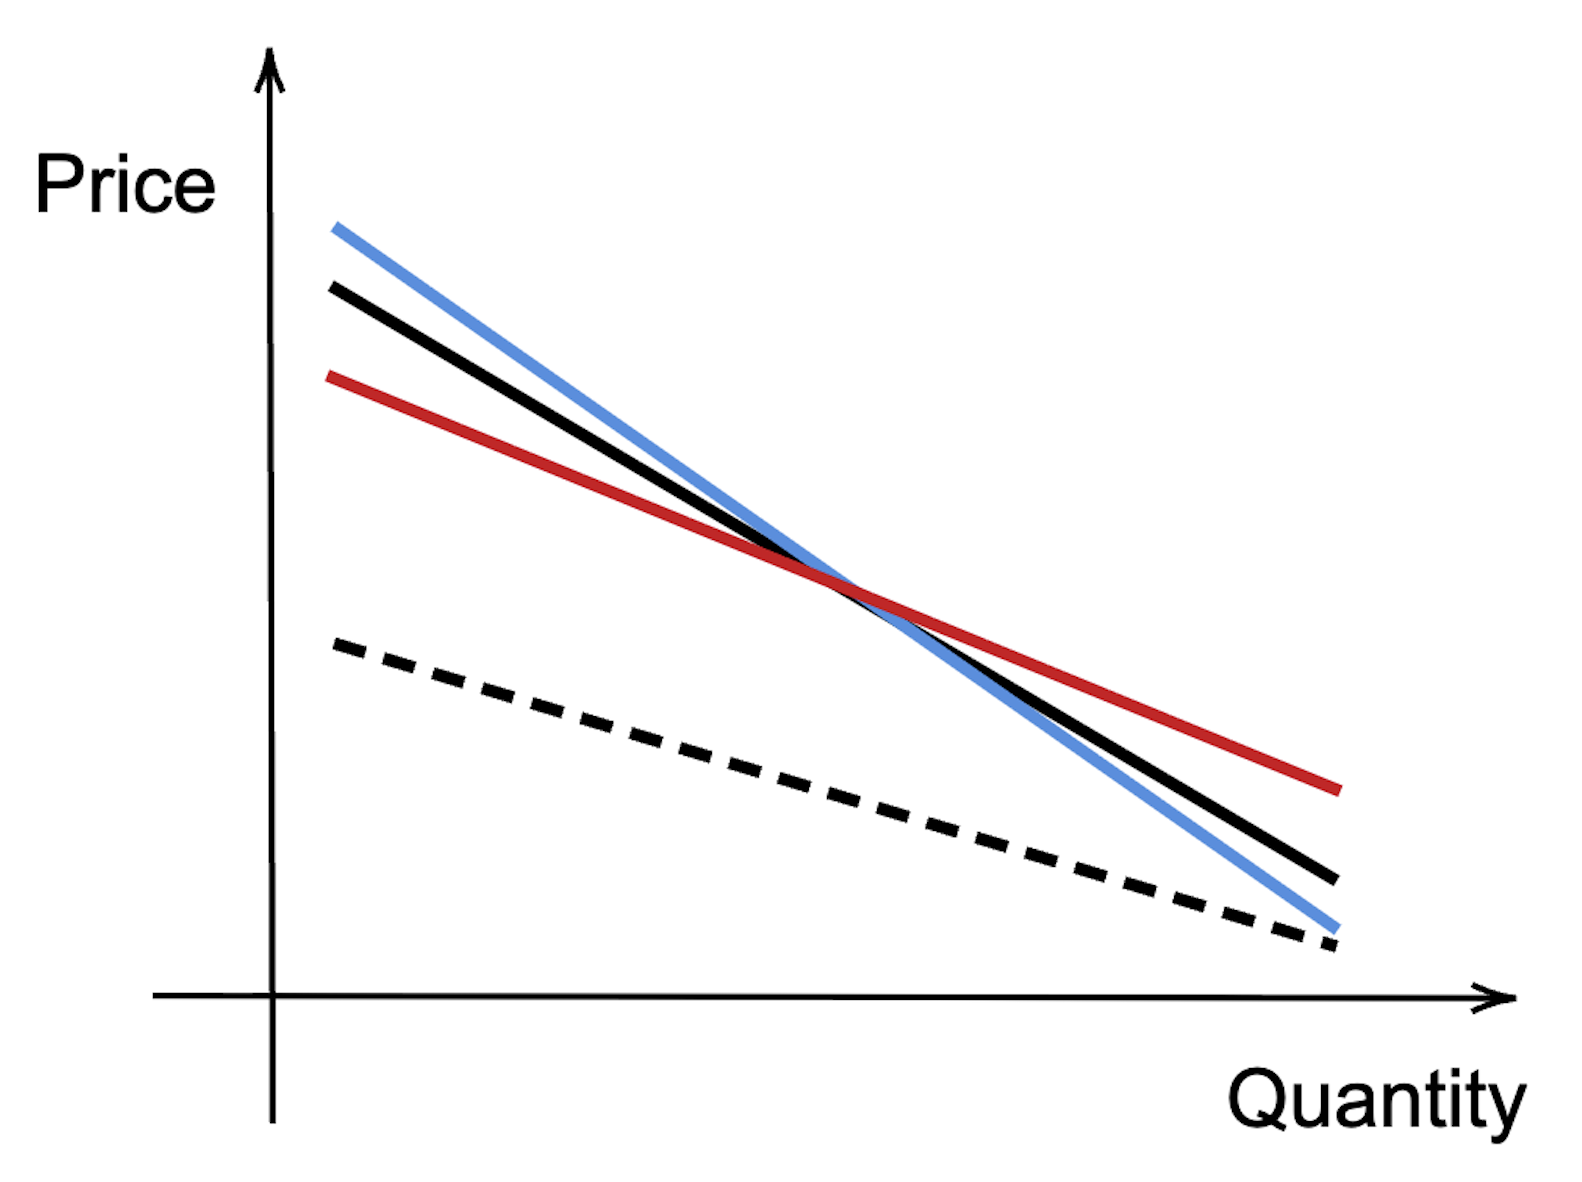
\includegraphics[width=0.5\linewidth]{demandcurves.png}
    \begin{original}
    \caption{Illustration of Changes in Demand Curves. The dashed black line is the original demand curve. The solid lines are three demand curves that increase surplus but have different elasticity effects: Solid black line keeps the same elasticities (a \textit{scaling}); solid red line increases elasticities (a \textit{flattening}); solid blue line decreases elasticities (a \textit{steepening}).}
    \end{original}
    \begin{translation}
    \caption{需求曲线变化示意图。黑色虚线为原始需求曲线。实线为三条增加剩余但具有不同弹性效应的需求曲线：黑色实线保持相同弹性（\textit{缩放}）；红色实线增加弹性（\textit{平坦化}）；蓝色实线降低弹性（\textit{陡峭化}）。}
    \end{translation}
    \label{fig:demandcurves}
\end{figure}

\begin{original}
As a simple illustration of the surplus-elasticity frontier, consider the classic example of selling a single good with different lotteries. A well-known result by \citet{Myerson1981} and \citet{riley1983optimal} shows that a single posted price is optimal and lotteries are not needed. An alternative way to see it via \Cref{thm:main} is to observe that different lotteries are simply \textit{\textbf{scalings}} of the original demand curve and have no effect on its elasticity. Thus, the surplus-elasticity frontier consists of only the degenerate lottery of getting the good with probability $1$, recovering the optimality of a posted price.
\end{original}
\begin{translation}
作为剩余-弹性前沿的一个简单示例，考虑经典的以不同彩票出售单一商品的例子。\citet{Myerson1981}和\citet{riley1983optimal}的一个著名结果表明，单一明码标价是最优的，不需要彩票。通过\Cref{thm:main}来看的另一种方式是观察到不同彩票仅仅是原始需求曲线的\textit{\textbf{缩放}}，对其弹性没有影响。因此，剩余-弹性前沿仅由以概率$1$获得商品的退化彩票组成，从而恢复了明码标价的最优性。
\end{translation}

\begin{original}
As another simple illustration, consider a monopolist who offers a product mix. Each product $x$ has two different dimensions of features, say \textit{\textbf{functionality}} and \textit{\textbf{design}}, $(\alpha, \beta) \in [0, 1]^2$. For any type $t\in[1, 2]$ consumer, their value is given by
\[v\big((\alpha, \beta), t\big) = (\alpha + t)^{\beta}\,.\]
Both features increase the consumers' values for the products, but the functionality dimension $\alpha$ \textit{\textbf{flattens}} the demand curve whereas the design dimension $\beta$ \textit{\textbf{steepens}} the demand curve.\footnote{Indeed, the demand curve for each product is simply
\[P(x, q) = (\alpha + F^{-1}(1-q))^{\beta}\]
where $F$ is the distribution of $t$, and hence increasing $\beta$ rotates the demand curves clockwise, whereas increasing $\alpha$ rotates the demand curve counterclockwise.
} \Cref{fig:demandcurves} illustrates. Thus, the surplus-elasticity frontier consists of only $\{(1, \beta)\}_{\beta\in[0,1]}$. \Cref{thm:main} says that the monopolist should offer a menu of products in which all the products have full functionality but they differ in the details of the design. Indeed, the incremental demand curves along the frontier $\{(1, \beta)\}_{\beta\in[0,1]}$ are also increasingly more inelastic as $\beta$ increases, and thus by \Cref{thm:main2}, $\{(1, \beta)\}_{\beta\in[0,1]}$  is optimal even if we allow for stochastic mechanisms, with optimal prices determined by upgrade pricing that prices against each incremental demand curve. The optimal prices depend on the distribution of consumer types $t$ (e.g., the income distribution), but the same menu stays optimal---indeed, as we discuss, the surplus-elasticity frontier is \textit{\textbf{agnostic}} to the type distribution.
\end{original}
\begin{translation}
作为另一个简单示例，考虑一个提供产品组合的垄断者。每种产品$x$有两个不同的特征维度，例如\textit{\textbf{功能性}}和\textit{\textbf{设计性}}，$(\alpha, \beta) \in [0, 1]^2$。对于任何类型$t\in[1, 2]$的消费者，其价值由下式给出
\[v\big((\alpha, \beta), t\big) = (\alpha + t)^{\beta}\,.\]
两种特征都提高了消费者对产品的估值，但功能性维度$\alpha$\textit{\textbf{平坦化}}了需求曲线，而设计性维度$\beta$\textit{\textbf{陡峭化}}了需求曲线。\footnote{实际上，每种产品的需求曲线就是
\[P(x, q) = (\alpha + F^{-1}(1-q))^{\beta}\]
其中$F$是$t$的分布，因此增加$\beta$会使需求曲线顺时针旋转，而增加$\alpha$会使需求曲线逆时针旋转。}\Cref{fig:demandcurves}对此进行了说明。因此，剩余-弹性前沿仅由$\{(1, \beta)\}_{\beta\in[0,1]}$组成。\Cref{thm:main}表明，垄断者应当提供一个产品菜单，其中所有产品都具有完全的功能性，但设计细节各不相同。实际上，沿前沿$\{(1, \beta)\}_{\beta\in[0,1]}$的增量需求曲线也随$\beta$增加而越来越缺乏弹性，因此由\Cref{thm:main2}，即便允许随机机制，$\{(1, \beta)\}_{\beta\in[0,1]}$也是最优的，最优价格由针对每条增量需求曲线的升级定价确定。最优价格取决于消费者类型$t$的分布（例如收入分布），但同一菜单保持最优——事实上，正如我们所讨论的，剩余-弹性前沿\textit{\textbf{不依赖于}}类型分布。
\end{translation}

\begin{original}
Perhaps surprisingly, the surplus-elasticity frontier remains optimal even if the principal does not just care about the revenue---\Cref{thm:main} turns out to hold identically even if the designer has redistributive preferences such as in optimal taxation or redistributive allocation problems, as long as the welfare weights are \textit{\textbf{redistributive}} in that they are weakly decreasing in the vertical types. Whenever a surplus-elasticity frontier exists, the \textit{\textbf{same}} frontier is optimal simultaneously for a broad set of objectives. In particular, in the above examples, the same menu would remain optimal even if the designer has redistributive preferences, and would remain optimal even among stochastic mechanisms.
\end{original}
\begin{translation}
或许令人惊讶的是，即便委托人不仅关心收入——\Cref{thm:main}结果同样适用于设计者具有再分配偏好的情形，例如最优税收或再分配分配问题，只要福利权重是\textit{\textbf{再分配性的}}，即它们在垂直类型上弱递减。只要存在一个剩余-弹性前沿，\textit{\textbf{同一}}前沿就同时对广泛的目标函数集是最优的。特别地，在上述例子中，即使设计者具有再分配偏好，同一菜单仍然是最优的，并且即使在随机机制中也仍然是最优的。
\end{translation}

\begin{original}
Because the pointwise comparisons of the demand curves and their elasticities are both partial orders, the surplus-elasticity frontier need not exist in general. However, we can generalize our comparisons by comparing a given demand curve to a collection of possibly randomized demand curves. We say that a collection of (randomized) demand curves \textit{\textbf{covers}} a given demand curve if they single-cross the given one from below individually and cover the graph of it collectively. \Cref{fig:covering} illustrates.
A menu of products $\X^\star$ is a \textit{\textbf{generalized frontier}} if the elements can be ordered such that there exists a corresponding stochastically ordered set of lotteries $\A \in \Delta(\X^\star)$ such that \textit{(i)} the demand curve of any element $x$ can be covered by a collection of (randomized) demand curves from $\A$ and \textit{(ii)} the demand curves of the elements in $\X^\star$ satisfy increasing differences. Our proof of \Cref{thm:main} actually shows that any surplus-elasticity frontier is a generalized frontier and any generalized frontier must be robustly optimal. Thus, we can readily weaken the requirement of finding a surplus-elasticity frontier to finding a generalized frontier  (\Cref{thm:main3}). Moreover, the conclusion of \Cref{thm:main2} also applies---if the incremental demand curves are ordered by elasticities along the generalized frontier, then it is also optimal among stochastic mechanisms.
\end{original}
\begin{translation}
由于需求曲线及其弹性的逐点比较都是偏序，剩余-弹性前沿一般情况下不一定存在。然而，我们可以通过将给定需求曲线与一组可能随机化的需求曲线进行比较来推广我们的比较。我们说一组（随机化的）需求曲线\textit{\textbf{覆盖}}一条给定的需求曲线，如果它们各自从下方单交给定的需求曲线，并且共同覆盖其图形。\Cref{fig:covering}对此进行了说明。
产品菜单 $\X^\star$ 是一个\textit{\textbf{广义前沿}}，如果元素可以被排序，使得存在一个对应的随机序彩票集合 $\A \in \Delta(\X^\star)$，满足\textit{(i)} 任何元素$x$的需求曲线都可以被来自$\A$的一组（随机化的）需求曲线覆盖，以及\textit{(ii)} $\X^\star$中元素的需求曲线满足递增差分。我们对\Cref{thm:main}的证明实际上表明，任何剩余-弹性前沿都是广义前沿，并且任何广义前沿必然是稳健最优的。因此，我们可以轻松地将寻找剩余-弹性前沿的要求弱化为寻找广义前沿(\Cref{thm:main3})。此外，\Cref{thm:main2}的结论同样适用——如果沿广义前沿的增量需求曲线按弹性排序，那么它在随机机制中也是最优的。
\end{translation}

\begin{original}
Besides the general economic insights, our main results turn out to be extremely helpful for identifying the optimal menus in a variety of important screening problems. We now explain our applications in detail.
\end{original}
\begin{translation}
除了一般的经济学洞见外，我们的主要结果对于在各种重要筛选问题中识别最优菜单极为有用。我们现在详细解释我们的应用。
\end{translation}

\begin{figure}[t]
    \centering
    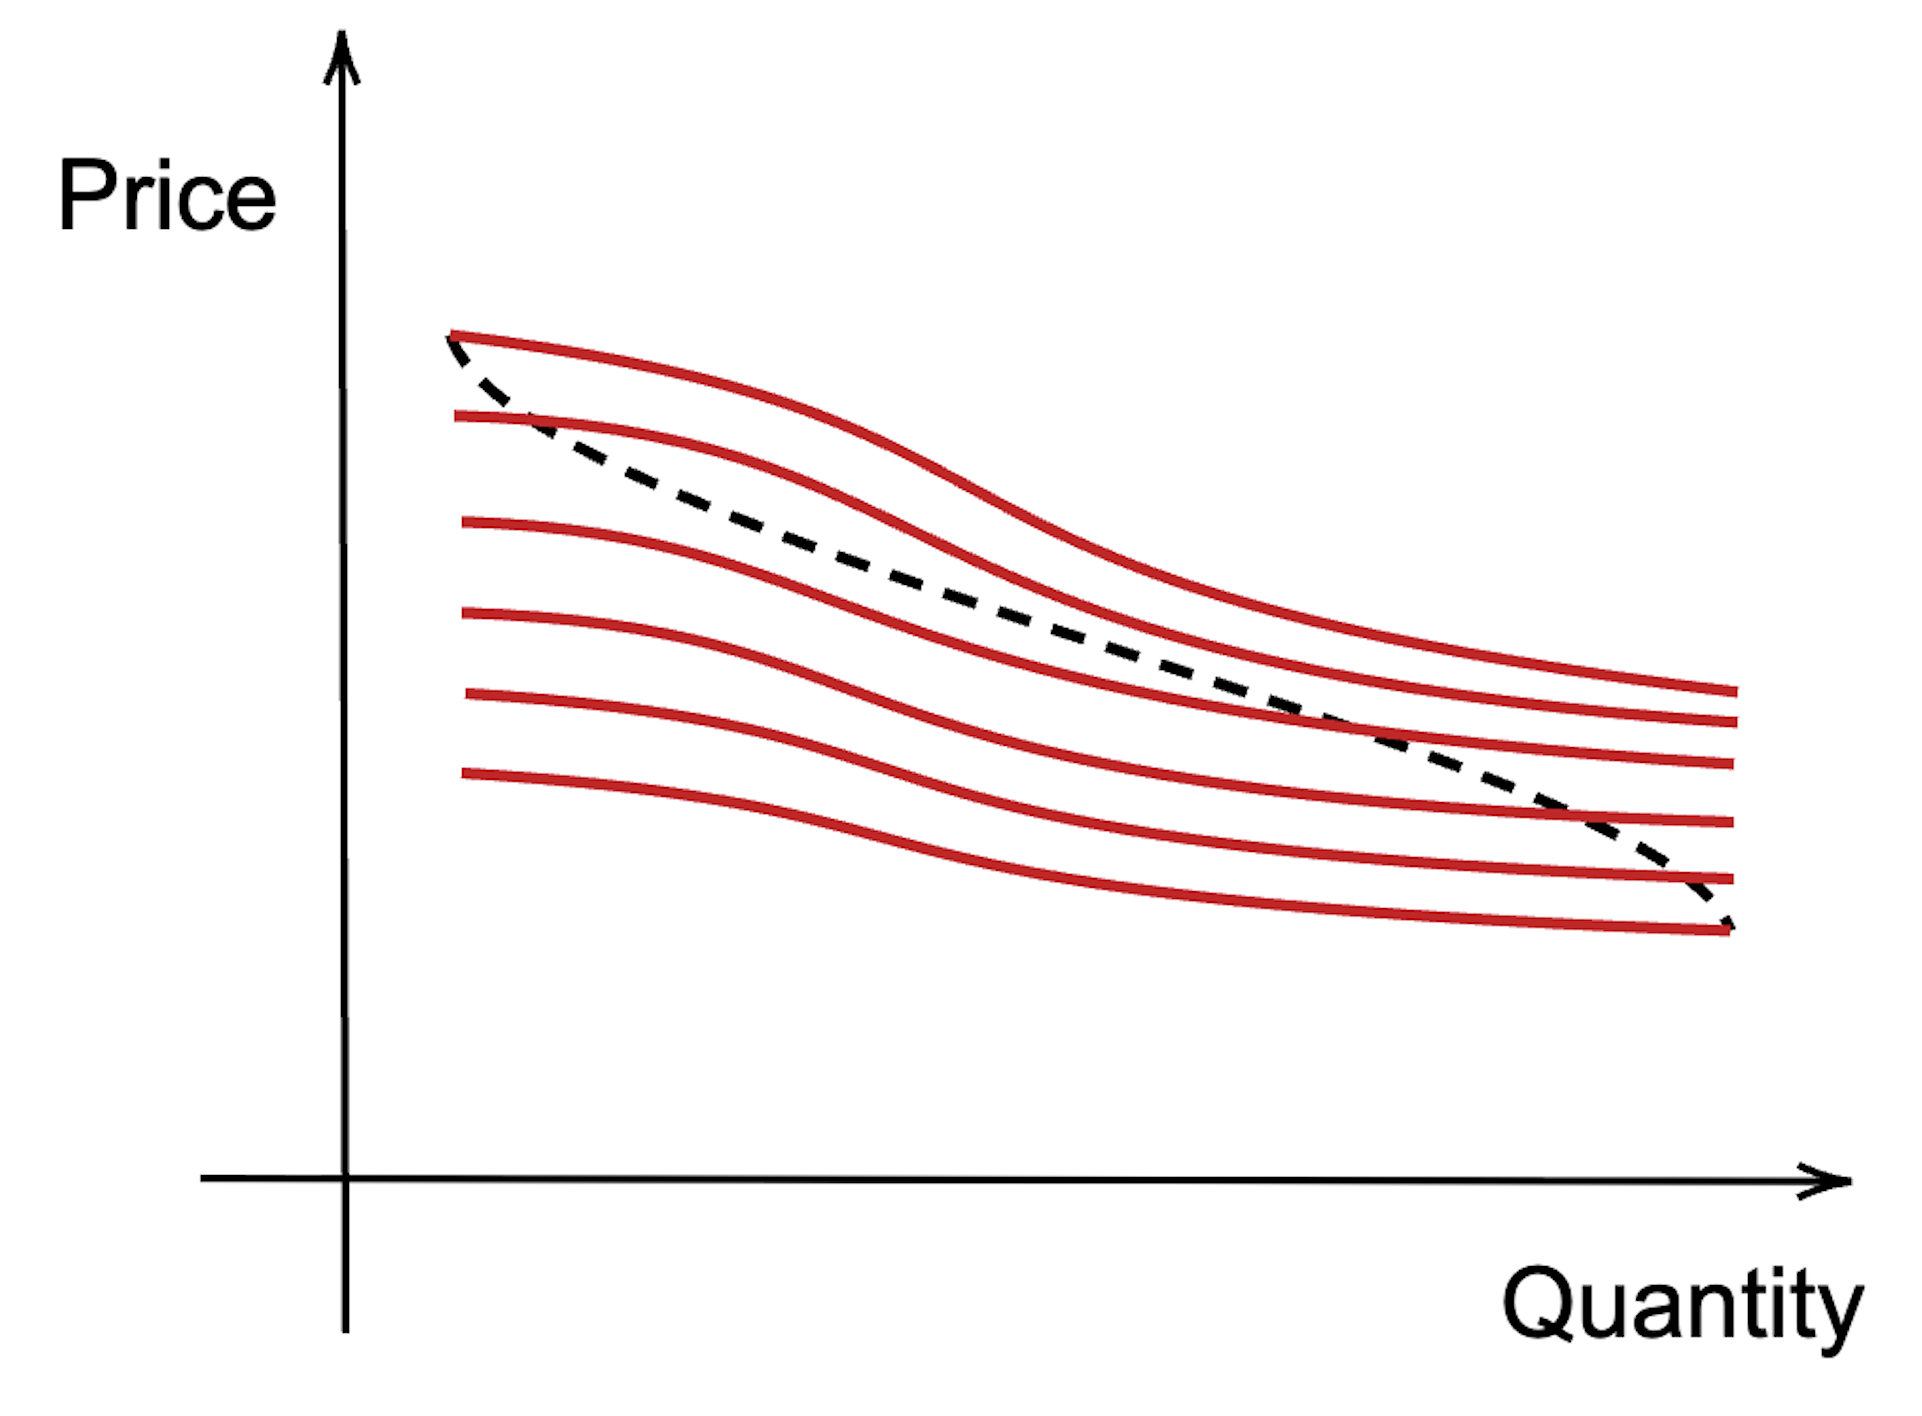
\includegraphics[width=0.5\linewidth]{covering.png}
    \begin{original}
    \caption{Illustration of Covering of a Demand Curve. The dashed black curve is the original demand curve. The collection of solid red demand curves \textit{covers} the original one by single-crossing it from below individually and covering it collectively. }
    \end{original}
    \begin{translation}
    \caption{需求曲线覆盖示意图。黑色虚线为原始需求曲线。红色实线需求曲线集合通过各自从下方单交原始需求曲线并共同覆盖来\textit{覆盖}原始需求曲线。}
    \end{translation}
    \label{fig:covering}
\end{figure}

\paragraph{Optimal Bundling.}\hspace{-2mm}\begin{original}Consider a designer who allocates bundles of a finite set of goods, where the consumers are vertically ordered and can have non-additive values. A common selling mechanism in such a setting is \textit{\textbf{nested bundling}} where more expensive bundles include all the goods of the less expensive ones. An immediate application of \Cref{thm:main} and \Cref{thm:main2} identifies a new condition (\textit{\textbf{robust nesting condition}}) for when nested bundling is optimal (\Cref{prop:nesting}). Nested bundling becomes optimal precisely when there is a nested menu that can span the surplus-elasticity frontier. The robust nesting condition complements and illuminates the demand conditions in \citet{yang2023nested} which depend on the type distribution and hold for profit maximization. Indeed, \citet{yang2023nested} considers the partial order defined by \textit{(i)} set inclusion and \textit{(ii)} sold-alone quantities, and shows that if the undominated bundles with respect to this partial order are nested, then this nested menu is optimal for profit maximization under regularity conditions. This can be understood via our results since a larger bundle generates a pointwise higher demand curve and a higher sold-alone quantity corresponds to a demand curve with a larger elastic region. Moreover, by virtue of our main results, \Cref{prop:nesting} shows that once there exists such a frontier, then the menu must be optimal for all type distributions and all redistributive welfare weights. This opens the door to apply results from the bundling literature to redistributive allocation problems. In particular, as another special case, we show that the \textit{\textbf{stochastic ratio-monotonicity condition}} of \citet{haghpanah2021pure} actually implies that pure bundling is optimal even if the designer is a social planner who has \textit{\textbf{redistributive}} preferences that favor agents who have lower values for the grand bundle (\Cref{cor:pure})---in this case, even if the designer cares more about poorer agents, the optimal mechanism is to use a blunt instrument by simply lowering the price for the grand bundle rather than offering smaller bundles to target poorer agents. This is precisely because the grand bundle itself forms the surplus-elasticity frontier under the ratio-monotonicity condition---the best way to control information rents for the richer agents turns out to fully exclude the poorer agents.
\end{original}
\begin{translation}
考虑一个设计者分配有限商品集中的捆绑，其中消费者被垂直排序且可以具有非可加估值。这种设定中常见的销售机制是\textit{\textbf{嵌套捆绑}}，即较贵的捆绑包含较便宜捆绑中的所有商品。\Cref{thm:main}和\Cref{thm:main2}的直接应用为嵌套捆绑何时最优识别出一个新的条件（\textit{\textbf{稳健嵌套条件}}）（\Cref{prop:nesting}）。当存在一个可以跨越剩余-弹性前沿的嵌套菜单时，嵌套捆绑就成为最优。稳健嵌套条件补充并阐明了\citet{yang2023nested}中的需求条件，后者依赖于类型分布且仅对利润最大化成立。实际上，\citet{yang2023nested}考虑了由\textit{(i)}集合包含和\textit{(ii)}单独出售数量定义的偏序，并证明如果对于这个偏序未被占优的捆绑是嵌套的，那么在正则性条件下，这个嵌套菜单对利润最大化是最优的。这可以通过我们的结果来理解，因为更大的捆绑产生逐点更高的需求曲线，而更高的单独出售数量对应于具有更大弹性区域的需求曲线。此外，凭借我们的主要结果，\Cref{prop:nesting}表明一旦存在这样的前沿，菜单必然对所有类型分布和所有再分配福利权重都是最优的。这为将捆绑文献的结果应用于再分配分配问题打开了大门。特别地，作为另一个特例，我们证明\citet{haghpanah2021pure}的\textit{\textbf{随机比率单调性条件}}实际上意味着纯捆绑即使在设计者是一个社会计划者且具有有利于对总捆绑估值较低的代理人的\textit{\textbf{再分配性}}偏好时也是最优的（\Cref{cor:pure}）——在这种情况下，即使设计者更关心较贫穷的代理人，最优机制也是使用一种钝化的工具，即简单地降低总捆绑的价格，而不是提供较小的捆绑来瞄准较贫穷的代理人。这恰恰是因为总捆绑本身在比率单调性条件下形成了剩余-弹性前沿——控制较富裕代理人信息租金的最佳方式被证明是完全排除较贫穷的代理人。
\end{translation}

\paragraph{Optimal Taxation.}\hspace{-2mm}\begin{original}Consider the optimal nonlinear taxation problem with quasilinear preferences (\citealt{diamond1998optimal}). Suppose the government has the ability to combine the \textit{\textbf{tax instruments}} with \textit{\textbf{costly screening}} to induce self-targeting in transfers. Would it be beneficial to do so?
\citet{Nichols1982b} shows that in such an environment, it is indeed \textit{\textbf{possible}} for the government to use socially wasteful ordeals to improve the net welfare because the ordeals can help with screening. Building on \citet{Nichols1982b}, we further explore this question by applying our main results. We show that there are two key forces that determine whether an ordeal should be used in the presence of tax instruments (\Cref{prop:ordeal}): \textit{(i)} As anticipated by \citet{Nichols1982b}, ordeals cannot be helpful if the higher ability types have lower costs from performing the ordeals; \textit{(ii)} even if the direction of sorting is correct, ordeals still cannot be helpful if an appropriately defined \textit{\textbf{take-up elasticity}} with respect to a small tax cut becomes lower when an ordeal is imposed. Intuitively, the reduction in surplus by an ordeal must be compensated via an increase in the screening effectiveness. In the absence of an ordeal, at the optimal tax schedule, the government would want to offer a marginal tax cut on the lower types which would also increase their labor supply but worry about the higher types shirking---an ordeal with \textit{\textbf{high}} take-up elasticity is helpful when combined with such a marginal tax cut---it increases the labor supply sensitivity of the lower types and dampens the incentive for shirking by the higher types. An ordeal with \textit{\textbf{low}} take-up elasticity cannot justify its distortion and hence results in taxation alone being optimal. As we discuss, the comparison here differs from the reforms that directly provide cash transfers conditional on the ordeals as studied in \citet*{yang2023comparison} and \citet*{rafkin2023self}, and highlights an appropriate notion of elasticity for assessing the screening gains from \textit{\textbf{combining}} ordeals and tax instruments.
\end{original}
\begin{translation}
考虑具有拟线性偏好的最优非线性税收问题（\citealt{diamond1998optimal}）。假设政府有能力将\textit{\textbf{税收工具}}与\textit{\textbf{代价高昂的筛选}}相结合以诱导转移支付中的自我瞄准。这样做是否有益？\citet{Nichols1982b}表明在这样的环境中，政府确实\textit{\textbf{有可能}}利用社会浪费性的考验来提高净福利，因为考验可以帮助筛选。在\citet{Nichols1982b}的基础上，我们通过应用主要结果进一步探讨了这个问题。我们证明存在两个关键力量决定在税收工具存在的情况下是否应该使用考验（\Cref{prop:ordeal}）：\textit{(i)} 正如\citet{Nichols1982b}所预期的，如果高能力类型执行考验的成本较低，考验将无助于改善福利；\textit{(ii)} 即使排序方向正确，如果施加考验后适当定义的\textit{\textbf{参与弹性}}相对于小额减税变得更低，考验仍然无济于事。直观上，考验造成的剩余减少必须通过筛选效果的提高来补偿。在没有考验的情况下，在最优税收计划下，政府希望为较低类型提供边际减税，这也会增加其劳动供给，但担心较高类型会逃避——具有\textit{\textbf{高}}参与弹性的考验与这种边际减税结合时是有帮助的——它增加了较低类型的劳动供给敏感性，并抑制了较高类型逃避的激励。具有\textit{\textbf{低}}参与弹性的考验无法证明其扭曲是合理的，因此导致仅靠税收是最优的。正如我们所讨论的，这里的比较不同于\citet*{yang2023comparison}和\citet*{rafkin2023self}所研究的直接以考验为条件提供现金转移的改革，并突出了评估\textit{\textbf{结合}}考验和税收工具所带来的筛选收益的适当弹性概念。
\end{translation}

\paragraph{Sequential Screening.}\hspace{-2mm}\begin{original}Consider the sequential screening problem introduced in \citet{Courty2000}. A seller contracts with a buyer on the sale of a good after the buyer has some initial estimate $t$ of their values $\theta$ but before they fully learn their values $\theta$. This is a canonical example of \textit{\textbf{dynamic mechanism design}} (\citealt*{Pavan2014}). In general, the optimal mechanism is sophisticated, involving a continuum of options, e.g., specifying different up-front fees for the possibility of having different refund options (\citealt{Courty2000}). In practice, however, even in many markets with buyer uncertainty, the selling mechanism is still very simple, often just a single \textit{\textbf{nonrefundable posted price}}. When is such a simple mechanism optimal in sequential screening?  Applying our main results, we show that a nonrefundable posted price is optimal if higher ex-ante types not only have higher expected willingness to pay (in the sense of FOSD) but also have greater uncertainty about their ex-post valuations in the sense of the \textit{\textbf{dispersive order on the log scale}} (\Cref{prop:sequential}).  Perhaps surprisingly, this is the case even though the principal could instead offer refunds to better target high types and extract surplus through a higher up-front fee. The key intuition is that since ex-post values are FOSD increasing in the ex-ante types, such a refund would have a leakage that attracts the lower types, which will then involve too much refund and eventually lead to a lower revenue for the principal. Note that here a refund with a high up-front fee actually \textit{\textbf{reduces}} the ex post surplus by reducing the consumption of consumers with lower ex post values, and hence it can be justified only by increasing the screening effectiveness by our main results. Yet under the log-dispersion order---which captures the elasticity of how ex post values vary with ex ante types---the screening effectiveness cannot be increased and hence a nonrefundable posted price is optimal. Even though sequential screening is a well-studied problem, we are not aware of any primitive condition under which a nonrefundable posted price is optimal. One reason is methodological: much of the dynamic mechanism design literature relies on the first-order approach under regularity assumptions that typically deliver fully separating allocations, so pooling/bunching mechanisms such as a nonrefundable posted price can be difficult to obtain without explicitly tracking the global incentive constraints.
\end{original}
\begin{translation}
考虑\citet{Courty2000}引入的序贯筛选问题。卖方在买方对其价值$\theta$有初步估计$t$之后、但尚未完全了解$\theta$之前，就商品的销售与买方签订合同。这是\textit{\textbf{动态机制设计}}的一个典型例子(\citealt*{Pavan2014})。一般来说，最优机制是复杂的，涉及连续统选项，例如，为拥有不同退款选项的可能性指定不同的预付费用(\citealt{Courty2000})。然而在实践中，即使在许多存在买方不确定性的市场中，销售机制仍然非常简单，通常只是一个单一的\textit{\textbf{不可退款明码标价}}。这种简单机制在序贯筛选中何时是最优的？应用我们的主要结果，我们证明如果较高事前类型不仅具有较高期望支付意愿（在一阶随机占优意义上），而且在对数尺度上的\textit{\textbf{离散序}}意义上对其事后估值具有更大的不确定性，则不可退款明码标价是最优的(\Cref{prop:sequential})。或许令人惊讶的是，即使委托人本可以通过提供退款来更好地瞄准高类型并通过更高的预付费来提取剩余，情况也是如此。关键的直觉是，由于事后价值在事前类型上是一阶随机占优递增的，这种退款将产生吸引低类型的泄漏，从而涉及过多的退款并最终导致委托人收入降低。注意，这里带有高预付费用的退款实际上\textit{\textbf{减少了}}事后剩余，因为它减少了事后价值较低的消费者的消费，因此只有通过我们的主要结果增加筛选效果才能证明其合理性。然而，在对数离散序下——它刻画了事后价值如何随事前类型变化的弹性——筛选效果无法增加，因此不可退款明码标价是最优的。尽管序贯筛选是一个被广泛研究的问题，但我们不知道有任何原始条件可以保证不可退款明码标价是最优的。一个原因是方法论上的：动态机制设计文献中的许多研究依赖于正则性假设下的一阶方法，这通常会导致完全分离的分配，因此如果不显式地跟踪全局激励约束，诸如不可退款明码标价之类的混同/集聚机制可能难以获得。
\end{translation}

\paragraph{Selling Information.}\hspace{-2mm}\begin{original}Fix a finite state space. Consider a designer selling \textit{\textbf{Blackwell experiments}} to an agent who has a decision problem to solve, just like in \citet*{bergemann2018design}. However, unlike \citet*{bergemann2018design}, suppose the agent has no private information about their prior belief about the state, but private information about their decision problems. Recall that every decision problem can be represented as a \textit{\textbf{convex indirect utility function}} of the posterior beliefs. Therefore, each agent of type $t$ is associated with a convex indirect utility function $u(\mu, t)$. We assume that the types are vertically ordered so that these indirect utility functions are increasing in the type $t$ compared to the no-information outside option. As observed in \citet*{bergemann2018design}, the space of Blackwell experiments is extremely rich as an allocation space. A commonly used class of signals is called \textit{\textbf{truth-or-noise signals}} (\citealt{lewis1994supplying})---such a signal either fully reveals the state  with some probability $\alpha$ or draws a completely noisy signal according to the prior with probability $1-\alpha$. The truth-or-noise signals are very simple in that they are controlled by a one-dimensional index $\alpha$, are Blackwell-monotone in $\alpha$, and generate posterior belief distributions with sparse supports. When are they optimal? Applying our main results, we show that in any symmetric environment, selling a menu of truth-or-noise signals is optimal if the agent's indirect utility function $u(\,\cdot\,, t)$ is \textit{\textbf{increasingly convex}} (in the Arrow-Pratt sense) in the posterior beliefs as the type increases (\Cref{prop:info}). This is the case where a higher vertical type (who has overall higher willingness to pay) tends to have decision problems that systematically depend \textit{\textbf{more sensitively}} on the state. In this case, the optimal menu---among menus of arbitrary Blackwell experiments---turns out to be a menu of truth-or-noise signals with a higher price for a higher signal-to-noise ratio. We also show that in the opposite case where the agent's indirect utility function $u(\,\cdot\,, t)$ is \textit{\textbf{increasingly concave}} in the posterior beliefs as the type increases, simply selling \textit{\textbf{full information}} is optimal. This is the case where a higher vertical type tends to have decision problems that systematically depend \textit{\textbf{less sensitively}} on the state. As this application shows, the existence of a screening frontier does not require a \textit{specific} directional assumption but only the existence of \textit{some} systematic structure of the agent's preferences.
\end{original}
\begin{translation}
固定一个有限状态空间。考虑一个设计者向有决策问题要解决的代理人销售\textit{\textbf{Blackwell实验}}，就像\citet*{bergemann2018design}中一样。然而，与\citet*{bergemann2018design}不同，假设代理人对状态的先验信念没有私人信息，但对其决策问题有私人信息。回顾每个决策问题可以表示为后验信念的\textit{\textbf{凸间接效用函数}}。因此，每个类型$t$的代理人关联一个凸间接效用函数$u(\mu, t)$。我们假设类型被垂直排序，使得这些间接效用函数在类型$t$上相对于无信息外部选项是递增的。正如\citet*{bergemann2018design}所观察到的，Blackwell实验的空间作为分配空间极其丰富。一类常用的信号被称为\textit{\textbf{真值或噪声信号}}（\citealt{lewis1994supplying}）——这种信号要么以某种概率$\alpha$完全揭示状态，要么以概率$1-\alpha$根据先验抽取完全噪声信号。真值或噪声信号非常简单，因为它们由一个一维指数$\alpha$控制，在$\alpha$上是Blackwell单调的，并产生具有稀疏支撑的后验信念分布。它们何时是最优的？应用我们的主要结果，我们表明在任何对称环境中，如果代理人的间接效用函数$u(\,\cdot\,, t)$在后验信念上随类型增加而\textit{\textbf{越来越凸}}（在Arrow-Pratt意义上），则销售真值或噪声信号菜单是最优的（\Cref{prop:info}）。这是较高垂直类型（具有总体上较高支付意愿）倾向于具有系统性地\textit{\textbf{更敏感地}}依赖于状态的决策问题的情况。在这种情况下，最优菜单——在任意Blackwell实验的菜单中——结果是一个真值或噪声信号菜单，信号噪声比越高价格越高。我们还表明，在相反的情况下，即代理人的间接效用函数$u(\,\cdot\,, t)$在后验信念上随类型增加而\textit{\textbf{越来越凹}}，简单地销售\textit{\textbf{完全信息}}是最优的。这是较高垂直类型倾向于具有系统性地\textit{\textbf{较不敏感地}}依赖于状态的决策问题的情况。如这一应用所示，筛选前沿的存在不要求\textit{特定的}方向性假设，而只要求代理人的偏好存在\textit{某种}系统性结构。
\end{translation}

\paragraph{Monopoly Regulation.}\hspace{-2mm}\begin{original}Our last application studies the classic problem of monopoly regulation, just like in \citet{Baron1982RegulatingCosts}. However, unlike \citet{Baron1982RegulatingCosts}, suppose the monopolist has \textit{\textbf{rich data}} about the consumers in the sense that the monopolist has a fine segmentation of the consumers and will engage in third-degree price discrimination in the absence of any regulation. Following \citet{strack2025non}, we model the data-rich monopolist as observing the consumers' values $\theta$ and designing any \textit{\textbf{pricing rule}} that specifies a randomized price for each consumer $\theta$. The monopolist privately observes their type $t$ which determines their cost $c(\theta, t)$ for serving any consumer type $\theta$. As in \citet{strack2025non}, this allows for interdependent costs which are very common in settings involving consumer data (e.g., credit markets and insurance markets). Consider a regulator who contracts with the monopolist on the pricing rules. As in \citet{Baron1982RegulatingCosts}, the regulator wants to maximize a weighted sum of the consumer and producer surplus but does not observe the cost type $t$ of the monopolist. The regulator hence will post a \textit{\textbf{menu of pricing rules}} with their associated subsidies or taxes. We say that a mechanism is a \textit{\textbf{uniform-pricing regulation}} if the menu consists of only deterministic pricing rules that do not depend on the consumers' type $\theta$. Equivalently, such a regulation imposes the \textit{\textbf{uniform pricing constraint}} for the firm and then simply taxes or subsidizes the firm according to the uniform price the firm chooses---under such a regulation, the determination of taxes/subsidies exactly collapses to the model of \citet{Baron1982RegulatingCosts}. Of course, without the tax instrument, it is clear that a uniform pricing constraint increases consumer surplus since otherwise the consumers are fully exploited. However, with a tax instrument, are uniform pricing regulations optimal? If not, what regulations are optimal? Applying our main results, we show that if the \textit{\textbf{total surplus}} $\theta - c(\theta, t)$ which depends on both consumer value $\theta$ and monopolist type $t$ is \textit{\textbf{log-submodular}}, then uniform pricing regulations are optimal (\Cref{prop:regulation}). In the opposite case, we show that if the total surplus is strictly \textit{\textbf{log-supermodular}}, then uniform pricing regulations cannot be optimal. Indeed, in that case, we show that \textit{\textbf{discriminatory pricing regulations}} are optimal---the regulator lets the monopolist fully utilize consumer data to price discriminate and design a suitable tax schedule to transfer the surplus to the consumers. As we discuss, our conditions capture the degree of adverse selection in the markets---in markets with \textit{\textbf{advantageous selection}} or \textit{\textbf{mild adverse selection}}, we have uniform pricing regulations being optimal; in markets with \textit{\textbf{severe adverse selection}}, the optimal regulation must involve discriminatory pricing. Our results apply here because the problem can again be equivalently cast as a screening problem with a rich allocation space---the space of consumer-contingent pricing rules---by our main results, with a right comparison of elasticities with respect to the monopolist type (which is exactly what the log-submodular/log-supermodular surplus condition captures), the optimal mechanism is described by a screening frontier in our sense which turns out to be either uniform pricing regulations or discriminatory pricing regulations.
\end{original}
\begin{translation}
我们最后一个应用研究垄断规制的经典问题，正如\citet{Baron1982RegulatingCosts}中一样。然而，与\citet{Baron1982RegulatingCosts}不同，假设垄断者拥有关于消费者的\textit{\textbf{丰富数据}}，即垄断者对消费者有精细的市场细分，且在没有任何规制的情况下会进行三级价格歧视。遵循\citet{strack2025non}，我们将数据丰富的垄断者建模为观察到消费者的价值$\theta$，并设计任何\textit{\textbf{定价规则}}为每个消费者$\theta$指定一个随机价格。垄断者私下观察到自己的类型$t$，这决定了其为任何消费者类型$\theta$提供服务的成本$c(\theta, t)$。正如\citet{strack2025non}中一样，这允许相互依赖的成本，这在涉及消费者数据的环境中非常常见（例如信贷市场和保险市场）。考虑一个规制者就定价规则与垄断者签订合同。正如\citet{Baron1982RegulatingCosts}中一样，规制者希望最大化消费者和生产者剩余的加权和，但不能观察到垄断者的成本类型$t$。因此，规制者将公布一个\textit{\textbf{定价规则菜单}}及其关联的补贴或税收。我们说一个机制是\textit{\textbf{统一定价规制}}，如果菜单仅由不依赖于消费者类型$\theta$的确定性定价规则组成。等价地，这种规制对企业施加\textit{\textbf{统一定价约束}}，然后简单地根据企业选择的统一价格对企业进行征税或补贴——在这种规制下，税收/补贴的决定恰好退化为\citet{Baron1982RegulatingCosts}的模型。当然，没有税收工具时，显然统一定价约束会增加消费者剩余，因为否则消费者会被完全压榨。然而，有了税收工具，统一定价规制是否是最优的？如果不是，什么规制是最优的？应用我们的主要结果，我们证明如果\textit{\textbf{总剩余}}$\theta - c(\theta, t)$——它同时依赖于消费者价值$\theta$和垄断者类型$t$——是\textit{\textbf{对数次模}}的，则统一定价规制是最优的(\Cref{prop:regulation})。在相反的情况下，我们证明如果总剩余是严格\textit{\textbf{对数超模}}的，那么统一定价规制不可能是最优的。实际上，在这种情况下，我们证明\textit{\textbf{歧视性定价规制}}是最优的——规制者让垄断者充分利用消费者数据进行价格歧视，并设计适当的税收计划将剩余转移给消费者。正如我们所讨论的，我们的条件刻画了市场中的逆向选择程度——在具有\textit{\textbf{有利选择}}或\textit{\textbf{温和逆向选择}}的市场中，统一定价规制是最优的；在具有\textit{\textbf{严重逆向选择}}的市场中，最优规制必须涉及歧视性定价。我们的结果适用于此，因为该问题又可以等价地表述为一个具有丰富分配空间——消费者依存的定价规则空间——的筛选问题，通过我们的主要结果，通过对垄断者类型弹性的正确比较（这正是对数次模/对数超模剩余条件所刻画的），最优机制由我们意义上的筛选前沿描述，结果要么是统一定价规制，要么是歧视性定价规制。
\end{translation}

\paragraph{Related Literature.}\hspace{-2mm}\begin{original}We view our main contributions as twofold. First, our conceptual contribution is to explicitly identify two intuitive channels, surplus and dispersion, measured by the levels and the elasticities of the sold-alone demand curves that together pin down the optimal menu in a general screening environment. Second, our methodological contribution is to show how various screening problems with rich allocation spaces can be characterized by identifying a suitable screening frontier that balances creating surplus and controlling information rents. We build on a large literature on multidimensional screening, most of which focuses on the optimal bundling problem. The model is traditionally set up as additive values with multidimensional types (\citealt*{McAfee1989MultiproductValues,Rochet1998, mcafee1988multidimensional, manelli2006bundling, daskalakis2017strong}) and turns out to be analytically and computationally intractable (\citealt{Rochet2003}; \citealt{daskalakis2014complexity}; \citealt{lahr2024extreme}). A recent line of work relaxes the additivity requirement and explores the consequences of \textit{\textbf{comonotonic type space}} where the consumer types are totally ordered (\citealt{haghpanah2021pure}; \citealt{ghili2021characterization}; \citealt{yang2023nested}). Our model builds heavily on this line of literature by fully embracing the one-dimensional type space and fully relaxing the allocation space requirement. In contemporaneous work, \citet{haghpanah2025screening} also study a model with an arbitrary allocation space but restrict attention to binary types, which allows them to study environments where types are not ordered.  Relatedly, \cite{pernoud2025bundling} characterize optimal mechanisms with non-ordered linear type spaces assuming additive values and provide a microfoundation for comonotonic types using equilibrium learning; \cite*{frick2024multidimensional} study the monopolist's problem with precise consumer data and provide structural results with linear type spaces.  Our proof method builds on and further develops the non-Myersonian approach in \citet{yang2022costly}. In particular, we generalize the \textit{\textbf{downward sufficiency theorem}} in \citet{yang2022costly} to allow for arbitrary redistributive welfare weights which, as our applications show, opens the door to apply results from multidimensional screening to recent redistributive allocation problems as well as classic optimal taxation and monopoly regulation problems.\footnote{See also \citet{doligalski2025optimal} for applying multidimensional screening techniques to taxation problems. There is also a substantial literature in public finance that studies taxation with multiple instruments (e.g., \citealt*{ferey2024sufficient}) or multidimensional heterogeneity (e.g., \citealt*{golosov2025optimal}).}
\end{original}
\begin{translation}
我们认为我们的主要贡献是双重的。首先，我们的概念贡献在于明确识别了两个直观的渠道——剩余和离散度，分别由单独出售需求曲线的水平和弹性来衡量，它们共同确定了一般筛选环境中的最优菜单。其次，我们的方法论贡献在于展示了如何通过识别一个适当的筛选前沿——它平衡了创造剩余和控制信息租金——来刻画具有丰富分配空间的各种筛选问题。我们建立在大量多维筛选文献的基础上，其中大多数关注最优捆绑问题。该模型传统上被设定为具有多维类型的可加价值(\citealt*{McAfee1989MultiproductValues,Rochet1998, mcafee1988multidimensional, manelli2006bundling, daskalakis2017strong})，并已被证明在分析和计算上是难以处理的(\citealt{Rochet2003}; \citealt{daskalakis2014complexity}; \citealt{lahr2024extreme})。最近的一系列工作放宽了可加性要求，并探索了消费者类型被完全排序的\textit{\textbf{共单调类型空间}}的后果(\citealt{haghpanah2021pure}; \citealt{ghili2021characterization}; \citealt{yang2023nested})。我们的模型在很大程度上建立在上述文献基础上，完全接纳一维类型空间并完全放宽了分配空间要求。在同期工作中，\citet{haghpanah2025screening}也研究了具有任意分配空间的模型，但将注意力限制在二元类型上，这使他们能够研究类型不被排序的环境。相关地，\cite{pernoud2025bundling}在假设可加价值的条件下刻画了非有序线性类型空间的最优机制，并利用均衡学习为共单调类型提供了微观基础；\cite*{frick2024multidimensional}研究了拥有精确消费者数据的垄断者问题，并在线性类型空间下提供了结构性结果。我们的证明方法建立在\citet{yang2022costly}中的非Myerson方法基础上并进一步发展了它。特别地，我们推广了\citet{yang2022costly}中的\textit{\textbf{向下充分性定理}}，使其允许任意的再分配福利权重，正如我们的应用所展示的，这为将多维筛选的结果应用于最近的再分配分配问题以及经典的最优税收和垄断规制问题打开了大门。\footnote{另见\citet{doligalski2025optimal}将多维筛选技术应用于税收问题。在公共财政领域也有大量文献研究多工具税收（例如\citealt*{ferey2024sufficient}）或多维异质性（例如\citealt*{golosov2025optimal}）。}
\end{translation}

\begin{original}
The remainder of the paper proceeds as follows. \Cref{sec:model} presents the model. \Cref{sec:main} presents the main results. \Cref{sec:proof} sketches the main proofs. \Cref{sec:application} presents the applications. \Cref{sec:conclude} concludes. \Cref{app:proof} contains the omitted proofs.
\end{original}
\begin{translation}
本文的剩余部分安排如下。\Cref{sec:model}介绍模型。\Cref{sec:main}介绍主要结果。\Cref{sec:proof}概述主要证明。\Cref{sec:application}介绍应用。\Cref{sec:conclude}作结。\Cref{app:proof}包含省略的证明。
\end{translation}

\begin{original}
\section{Model}\label{sec:model}
\end{original}
\begin{translation}
\section{模型}\label{sec:model}
\end{translation}

\begin{original}
A principal screens an agent. The allocation space is a compact metric space $\mathcal{X} \ni x$. The agent has a one-dimensional type $t \in \mathcal{T}:=[\underline{t}, \overline{t}]$, distributed according to a continuously differentiable $F$ with a positive density $f$. The agent has quasilinear preferences, given by
\[v(x, t) - p\]
where $p$ is the payment. We assume that the agent's value function $v(x, t)$ is strictly increasing and differentiable in $t$ with $v_t(x, t)$ continuous on $\mathcal{X} \times \mathcal{T}$.
\end{original}
\begin{translation}
一个委托人筛选一个代理人。分配空间是一个紧度量空间 $\mathcal{X} \ni x$。代理人具有一维类型 $t \in \mathcal{T}:=[\underline{t}, \overline{t}]$，按照连续可微的 $F$ 分布，具有正密度 $f$。代理人具有拟线性偏好，由下式给出
\[v(x, t) - p\]
其中 $p$ 是支付。我们假设代理人的价值函数 $v(x, t)$ 在 $t$ 上严格递增且可微，$v_t(x, t)$ 在 $\mathcal{X} \times \mathcal{T}$ 上连续。
\end{translation}

\begin{original}
The principal wants to maximize a weighted average of welfare and revenue. By the revelation principle, it is without loss of generality to consider direct-revelation mechanisms. A \textit{\textbf{(direct-revelation) mechanism}} is a measurable map
\[(x, p): \mathcal{T} \rightarrow \mathcal{X} \times \R \]
that satisfies the usual incentive compatibility (IC) and individual rationality (IR) constraints:
\begin{align*}
    v(x(t), t) - p(t) &\geq     v(x(\hat{t}), t) - p(\hat{t})  &&\text{for all $t, \hat{t} \in \mathcal{T}$\,;} \\
   v(x(t), t) - p(t) &\geq    0  &&\text{for all $t \in \mathcal{T}$}\,.
\end{align*}
Let $\emptyset$ denote the \textit{\textbf{outside option}} that gives all types $0$ payoff. To simplify notation, we augment $\X$ with the outside option $\emptyset$. Two mechanisms are \textit{\textbf{equivalent}} if they differ on a zero-measure set of types. Formally, the principal's objective is given by a weighted average of welfare and revenue:
\[\E\big[\lambda (t) \big(v(x(t), t) - p(t)\big)\big] + \E\big[p(t)\big]\,,\]
where $\lambda(\,\cdot\,) \geq 0$ is a continuous \textit{\textbf{welfare weight function}}.
We assume $\E[\lambda(t)] \leq 1$.\footnote{If $\E[\lambda(t)] > 1$, the principal's problem would have unbounded value by scaling up a lump sum transfer to the agent.} We assume that the welfare weights are \textit{\textbf{redistributive}} in the sense that $\lambda(t)$ is non-increasing in $t$.\footnote{Since the agents' preferences are pinned down by $t$, the formulation is equivalent to having $(\lambda, t)$ jointly distributed with $\E[\lambda \mid t]$ being non-increasing in $t$.} With constant $\lambda$, this objective captures any weighted average of surplus and revenue. With varying $\lambda$, this objective allows for optimal taxation (corresponding to $\E[\lambda(t)] = 1$) or redistributive allocation applications where the welfare weight is weakly higher for the lower types. When $\lambda = 0$, the principal is profit maximizing, in which case if there is a production cost $C(x)$ for providing allocation $x$, we can without loss of generality normalize it to be $0$ by defining $\tilde{v}(x, t) = v(x, t) - C(x)$.\footnote{In particular, all of our demand curves are defined as net of the production costs.}
\end{original}
\begin{translation}
委托人希望最大化福利和收入的加权平均。根据显示原理，考虑直接显示机制不失一般性。一个\textit{\textbf{（直接显示）机制}}是一个可测映射
\[(x, p): \mathcal{T} \rightarrow \mathcal{X} \times \R \]
满足通常的激励相容（IC）和个体理性（IR）约束：
\begin{align*}
    v(x(t), t) - p(t) &\geq     v(x(\hat{t}), t) - p(\hat{t})  &&\text{对所有 $t, \hat{t} \in \mathcal{T}$\,;} \\
   v(x(t), t) - p(t) &\geq    0  &&\text{对所有 $t \in \mathcal{T}$}\,.
\end{align*}
令 $\emptyset$ 表示赋予所有类型 $0$ 收益的\textit{\textbf{外部选项}}。为简化记号，我们用外部选项 $\emptyset$ 扩展 $\X$。如果两个机制在类型的零测集上不同，则称它们是\textit{\textbf{等价的}}。正式地，委托人的目标由福利和收入的加权平均给出：
\[\E\big[\lambda (t) \big(v(x(t), t) - p(t)\big)\big] + \E\big[p(t)\big]\,,\]
其中 $\lambda(\,\cdot\,) \geq 0$ 是一个连续的\textit{\textbf{福利权重函数}}。
我们假设 $\E[\lambda(t)] \leq 1$。\footnote{如果 $\E[\lambda(t)] > 1$，通过放大对代理人的一次性总额转移，委托人的问题将具有无界值。}我们假设福利权重是\textit{\textbf{再分配性的}}，即 $\lambda(t)$ 在 $t$ 上非递增。\footnote{由于代理人的偏好由 $t$ 确定，该表述等价于 $(\lambda, t)$ 联合分布且 $\E[\lambda \mid t]$ 在 $t$ 上非递增。}当 $\lambda$ 为常数时，该目标涵盖了剩余和收入的任意加权平均。当 $\lambda$ 变化时，该目标允许最优税收（对应 $\E[\lambda(t)] = 1$）或再分配分配应用，其中较低类型的福利权重弱较高。当 $\lambda = 0$ 时，委托人是利润最大化的，在这种情况下，如果提供分配 $x$ 存在生产成本 $C(x)$，我们可以通过定义 $\tilde{v}(x, t) = v(x, t) - C(x)$ 将其标准化为 $0$ 而不失一般性。\footnote{特别地，我们所有的需求曲线都被定义为扣除生产成本后的净值。}
\end{translation}

\begin{original}
A \textit{\textbf{menu}} $\mathcal{Y}$ is any subset of $\mathcal{X}$ (which we assume also includes the outside option $\varnothing$).\footnote{To simplify notation, we omit the inclusion of $\emptyset$ from a menu whenever it is clear.}
A menu $\mathcal{Y}$ is \textit{\textbf{optimal}} if there exists an optimal mechanism $(x, p)$ such that $x(t) \in \mathcal{Y}$ for all types $t$. Since the space of allocations $\mathcal{X}$ is abstract, we can allow for stochastic mechanisms by directly encoding them in $\mathcal{X}$. However, some of our results have the feature that they only require comparisons for the elements in $\mathcal{X}$ to imply optimality even if the allocation space is extended to $\Delta(\mathcal{X})$. Thus, we explicitly say that a menu $\mathcal{Y}$ is \textit{\textbf{optimal among stochastic mechanisms}} if there exists a mechanism $(x, p)$ such that $x(t) \in \mathcal{Y}$ for all types $t$ and $(x, p)$ is optimal among all IC and IR mechanisms mapping from $\mathcal{T}$ to $\Delta(\mathcal{X}) \times \R$ (assuming risk neutrality).
\end{original}
\begin{translation}
一个\textit{\textbf{菜单}} $\mathcal{Y}$ 是 $\mathcal{X}$ 的任何子集（我们假设它也包括外部选项 $\varnothing$）。\footnote{为简化记号，当含义清楚时我们省略菜单中 $\emptyset$ 的包含。}
如果存在一个最优机制 $(x, p)$ 使得对所有类型 $t$ 有 $x(t) \in \mathcal{Y}$，则称菜单 $\mathcal{Y}$ 是\textit{\textbf{最优的}}。由于分配空间 $\mathcal{X}$ 是抽象的，我们可以通过直接将其编码在 $\mathcal{X}$ 中来允许随机机制。然而，我们的一些结果是，它们仅需要对 $\mathcal{X}$ 中元素的比较即可得出最优性，即使分配空间扩展到 $\Delta(\mathcal{X})$ 也是如此。因此，我们明确地说一个菜单 $\mathcal{Y}$ 是\textit{\textbf{在随机机制中最优的}}，如果存在一个机制 $(x, p)$ 使得对所有类型 $t$ 有 $x(t) \in \mathcal{Y}$，且 $(x, p)$ 在所有从 $\mathcal{T}$ 映射到 $\Delta(\mathcal{X}) \times \R$ 的IC和IR机制中是最优的（假设风险中性）。
\end{translation}

\begin{original}
Let $P(x, q)$ be the \textit{\textbf{demand curve}} for allocation $x$ when $x$ is sold alone:
\[P(x, q) := v(x, F^{-1}(1 - q))\,.\]
Let $\eta(x, q)$ be the corresponding \textit{\textbf{elasticity curve}} for allocation $x$:
\[\eta(x, q) := \big|\frac{\d \log P(x, q)}{\d \log q}\big|^{-1} \,.\]
Note that a higher $\eta$ represents a more elastic demand curve. For any $x, x' \in \mathcal{X}$, we write
\[x \preceq_{\text{surplus}} x' \,\,\,\text{ if $P(x, q) \leq P(x', q)$ for all $q$}\,;\]
and
\[x \preceq_{\text{elasticity}} x' \,\,\,\text{ if $\eta(x, q) \leq \eta(x', q)$ for all $q$}\,.\]
We write $\prec_{\text{surplus}}$ or $\prec_{\text{elasticity}}$ if the above inequalities hold strictly for all $q \in (0, 1)$. Note that for the above elasticity comparison to be well defined, we implicitly assume that $P(x, q) > 0$, i.e., $v(x, t) > 0$ for any $x \neq \emptyset$. We will relax this assumption for our notion of generalized frontiers which replace elasticity comparisons with single-crossing comparisons of demand curves.
\end{original}
\begin{translation}
令 $P(x, q)$ 为分配 $x$ 单独出售时的\textit{\textbf{需求曲线}}：
\[P(x, q) := v(x, F^{-1}(1 - q))\,.\]
令 $\eta(x, q)$ 为分配 $x$ 相应的\textit{\textbf{弹性曲线}}：
\[\eta(x, q) := \big|\frac{\d \log P(x, q)}{\d \log q}\big|^{-1} \,.\]
注意较高的 $\eta$ 表示更具弹性的需求曲线。对任意 $x, x' \in \mathcal{X}$，我们记
\[x \preceq_{\text{surplus}} x' \,\,\,\text{ 如果对所有 $q$ 有 $P(x, q) \leq P(x', q)$}\,;\]
以及
\[x \preceq_{\text{elasticity}} x' \,\,\,\text{ 如果对所有 $q$ 有 $\eta(x, q) \leq \eta(x', q)$}\,.\]
如果上述不等式对所有 $q \in (0, 1)$ 严格成立，我们写 $\prec_{\text{surplus}}$ 或 $\prec_{\text{elasticity}}$。注意为使上述弹性比较有意义，我们隐含假设 $P(x, q) > 0$，即对任何 $x \neq \emptyset$ 有 $v(x, t) > 0$。对于我们的广义前沿概念，我们将放宽这一假设，该概念用需求曲线的单交比较代替弹性比较。
\end{translation}

\begin{original}
\section{Main Results}\label{sec:main}
\end{original}
\begin{translation}
\section{主要结果}\label{sec:main}
\end{translation}

\begin{original}
\subsection{Optimality of Surplus-Elasticity Frontier}
\end{original}
\begin{translation}
\subsection{剩余-弹性前沿的最优性}
\end{translation}

\begin{original}
A compact subset $\mathcal{X}^\star \subseteq \mathcal{X}$ is a \textit{\textbf{surplus-elasticity frontier}} if:
\begin{itemize}
    \item[\textit{(i)}] for any $x \not\in \mathcal{X}^\star$, there exists $x' \in \mathcal{X}^\star$ such that
    \[\text{ $x \preceq_{\text{surplus}} x'$ and $x \preceq_{\text{elasticity}} x'$ } \,\,;\]
    \item[\textit{(ii)}] there exists an index set $S\subset \R$ such that $\X^\star = \{x_s\}_{s\in S}$ and for all $s < s'$
    \[x_{s} \prec_{\text{surplus}} x_{s'} \text{ and } x_{s} \succ_{\text{elasticity}} x_{s'}\,\,.\]
\end{itemize}
\end{original}
\begin{translation}
一个紧子集 $\mathcal{X}^\star \subseteq \mathcal{X}$ 是一个\textit{\textbf{剩余-弹性前沿}}，如果：
\begin{itemize}
    \item[\textit{(i)}] 对任意 $x \not\in \mathcal{X}^\star$，存在 $x' \in \mathcal{X}^\star$ 使得
    \[\text{ $x \preceq_{\text{surplus}} x'$ 且 $x \preceq_{\text{elasticity}} x'$ } \,\,;\]
    \item[\textit{(ii)}] 存在一个指标集 $S\subset \R$ 使得 $\X^\star = \{x_s\}_{s\in S}$ 且对所有 $s < s'$
    \[x_{s} \prec_{\text{surplus}} x_{s'} \text{ 且 } x_{s} \succ_{\text{elasticity}} x_{s'}\,\,.\]
\end{itemize}
\end{translation}

\begin{original}
Our first main result says that any surplus-elasticity frontier is an optimal menu.
\end{original}
\begin{translation}
我们的第一个主要结果表明，任何剩余-弹性前沿都是最优菜单。
\end{translation}

\begin{theorem}\label{thm:main}
\begin{original}
Any surplus-elasticity frontier is an optimal menu.
\end{original}
\begin{translation}
任何剩余-弹性前沿都是最优菜单。
\end{translation}
\end{theorem}

\begin{original}
The proof of \Cref{thm:main} is in the appendix. We sketch the proof in \Cref{sec:proof}.

We make a few remarks about this result here.

First, note that
\[x \preceq_{\text{surplus}} x'  \iff v(x, t) \leq v(x', t) \text{ for all $t$}\]
and
\[\qquad \qquad \quad \,\, x \preceq_{\text{elasticity}} x'  \iff \frac{\d}{\d t} \log v(x, t) \geq \frac{\d}{\d t} \log v(x', t) \text{ for all $t$}\,.\]
Thus, the definition of a surplus-elasticity frontier does not depend on the type distribution $F$. Moreover, note that the definition of the frontier is also agnostic to the welfare weights $\lambda(t)$. Perhaps surprisingly,  \Cref{thm:main} asserts that the \textit{\textbf{same}} frontier would be optimal across all type distributions $F$ and all weakly decreasing welfare weights $\lambda(t)$.
\end{original}
\begin{translation}
\Cref{thm:main}的证明在附录中。我们在\Cref{sec:proof}中概述了该证明。

我们在此对该结果作几点说明。

首先，注意
\[x \preceq_{\text{surplus}} x'  \iff v(x, t) \leq v(x', t) \text{ 对所有 $t$}\]
且
\[\qquad \qquad \quad \,\, x \preceq_{\text{elasticity}} x'  \iff \frac{\d}{\d t} \log v(x, t) \geq \frac{\d}{\d t} \log v(x', t) \text{ 对所有 $t$}\,.\]
因此，剩余-弹性前沿的定义不依赖于类型分布 $F$。此外，注意前沿的定义也不依赖于福利权重 $\lambda(t)$。或许令人惊讶的是，\Cref{thm:main}断言\textit{\textbf{同一}}前沿在所有类型分布 $F$ 和所有弱递减福利权重 $\lambda(t)$ 下都是最优的。
\end{translation}

\begin{original}
Second, to further illustrate the intuition of the surplus-elasticity frontier, we connect the two orders to two stochastic orders. Let $\preceq_{\text{fosd}}$ denote the \textit{\textbf{first-order stochastic dominance order}}. Let $\preceq_{\text{disp}}$ denote the \textit{\textbf{dispersive order}} (\citealt{muller2002comparison}), i.e., two random variables $X \preceq_{\text{disp}} Y$ if $F^{-1}_X(q') - F^{-1}_X(q) \leq F^{-1}_Y(q') - F^{-1}_Y(q)$ for all $q < q' \in [0, 1]$. Let $V^x$ denote the random variable induced by $v(x, t)$. Note that
\[x \preceq_{\text{surplus}} x'  \iff V^x \preceq_{\text{fosd}} V^{x'}\]
and
\[\qquad \, \, \,\, x \preceq_{\text{elasticity}} x'  \iff \log V^{x} \succeq_{\text{disp}} \log V^{x'}\,.\]
In particular, the elasticity comparison is equivalent to the dispersion comparison according to the dispersive order on the log scale. Intuitively, this captures the level of information rents to the agents.\footnote{See also \citet*{yang2023comparison} who show that the log-level dispersion is important in understanding the rent an agent can secure in one-dimensional linear screening problems.}
\end{original}
\begin{translation}
第二，为进一步说明剩余-弹性前沿的直觉，我们将这两个序与两个随机序联系起来。令 $\preceq_{\text{fosd}}$ 表示\textit{\textbf{一阶随机占优序}}。令 $\preceq_{\text{disp}}$ 表示\textit{\textbf{离散序}} (\citealt{muller2002comparison})，即两个随机变量 $X \preceq_{\text{disp}} Y$ 如果对所有 $q < q' \in [0, 1]$ 有 $F^{-1}_X(q') - F^{-1}_X(q) \leq F^{-1}_Y(q') - F^{-1}_Y(q)$。令 $V^x$ 表示由 $v(x, t)$ 导出的随机变量。注意
\[x \preceq_{\text{surplus}} x'  \iff V^x \preceq_{\text{fosd}} V^{x'}\]
且
\[\qquad \, \, \,\, x \preceq_{\text{elasticity}} x'  \iff \log V^{x} \succeq_{\text{disp}} \log V^{x'}\,.\]
特别地，弹性比较等价于对数尺度上离散序意义上的离散度比较。直观上，这刻画了代理人的信息租金水平。\footnote{另见\citet*{yang2023comparison}，他们表明对数水平的离散度对于理解代理人在一维线性筛选问题中能获得的租金是重要的。}
\end{translation}

\begin{original}
Third, along the surplus-elasticity frontier, note that the agent's preferences satisfy \textit{\textbf{increasing differences}}: For any $s < s'$,
\[x_{s} \prec_{\text{surplus}} x_{s'} \text{ and } x_{s} \succ_{\text{elasticity}} x_{s'} \implies \text{$v(x_{s'}, t) - v(x_s, t)$ is strictly increasing in $t$}\,.\footnote{Indeed, for all $s < s'$, we can write $v_t(x_s, t) = \frac{v_t(x_s, t)}{v(x_s, t)} \cdot v(x_s, t) < \frac{v_t(x_{s'}, t)}{v(x_{s'}, t)} \cdot v(x_{s'}, t) = v_t(x_{s'}, t)$,
where the strict inequality uses that the menu $\X^\star$ is a surplus-elasticity frontier and that $0 < v(x_{s}, t) \leq v(x_{s'}, t)$. }\]
Thus, the pricing problem along the frontier can always be solved via well-known one-dimensional screening methods.
\end{original}
\begin{translation}
第三，沿剩余-弹性前沿，注意代理人的偏好满足\textit{\textbf{递增差分}}：对任意 $s < s'$，
\[x_{s} \prec_{\text{surplus}} x_{s'} \text{ 且 } x_{s} \succ_{\text{elasticity}} x_{s'} \implies \text{$v(x_{s'}, t) - v(x_s, t)$ 在 $t$ 上严格递增}\,.\footnote{实际上，对所有 $s < s'$，我们可以写 $v_t(x_s, t) = \frac{v_t(x_s, t)}{v(x_s, t)} \cdot v(x_s, t) < \frac{v_t(x_{s'}, t)}{v(x_{s'}, t)} \cdot v(x_{s'}, t) = v_t(x_{s'}, t)$，
其中严格不等式利用了菜单 $\X^\star$ 是剩余-弹性前沿以及 $0 < v(x_{s}, t) \leq v(x_{s'}, t)$。}\]
因此，沿前沿的定价问题总是可以通过众所周知的一维筛选方法求解。
\end{translation}

\begin{original}
Fourth, a particular special case is when the frontier consists of only one element, say $\overline{x}$. That is, element $\overline{x}$ generates more surplus than any other element in $\mathcal{X}$ and has a more elastic demand curve than that of any other element in $\mathcal{X}$. \Cref{thm:main} says that it is optimal to simply offer this maximal-surplus element, i.e., no screening distortion is needed. This connects to the optimality of pure bundling as studied in \citet{haghpanah2021pure}. Indeed, note that
\[x \preceq_{\text{elasticity}} x'  \iff v(x, t)/v(x', t) \text{ is nondecreasing in $t$}\,.\]
The main result of \citet{haghpanah2021pure} establishes that if $v(b, t) / v(\overline{b}, t)$ is nondecreasing in $t$ for all bundles $b$, then selling only the grand bundle $\overline{b}$ is profit maximizing. This can be seen from \Cref{thm:main} by taking $\mathcal{X}$ to be the space of lotteries over bundles, and observing that mixtures of deterministic bundles yield a randomized bundle with demand curve pointwise below that of the grand bundle, and pointwise more inelastic than that of the grand bundle given the ratio-monotonicity condition---the surplus-elasticity frontier consists of only the grand bundle. Perhaps surprisingly, \Cref{thm:main} shows that the identical ratio-monotonicity condition of \citet{haghpanah2021pure} actually implies the optimality of pure bundling (or equivalently, no screening distortion besides exclusion) for arbitrary redistributive welfare weights. We discuss more applications to optimal bundling in \Cref{sec:application}.
\end{original}
\begin{translation}
第四，一个特殊情形是当前沿仅由一个元素组成，例如 $\overline{x}$。也就是说，元素 $\overline{x}$ 比 $\mathcal{X}$ 中的任何其他元素产生更多的剩余，并且具有比 $\mathcal{X}$ 中任何其他元素更具弹性的需求曲线。\Cref{thm:main} 表明，简单地提供这个最大剩余元素是最优的，即不需要筛选扭曲。这与\citet{haghpanah2021pure}研究的纯捆绑最优性相关联。实际上，注意
\[x \preceq_{\text{elasticity}} x'  \iff v(x, t)/v(x', t) \text{ 在 $t$ 上非递减}\,.\]
\citet{haghpanah2021pure}的主要结果确立了如果对所有捆绑 $b$，$v(b, t) / v(\overline{b}, t)$ 在 $t$ 上非递减，则仅销售总捆绑 $\overline{b}$ 是利润最大化的。这可以从\Cref{thm:main}中看出，取 $\mathcal{X}$ 为捆绑上的彩票空间，并观察到确定性捆绑的混合产生一个随机化捆绑，其需求曲线逐点低于总捆绑的需求曲线，并且在比率单调性条件下逐点比总捆绑的需求曲线更缺乏弹性——剩余-弹性前沿仅由总捆绑组成。或许令人惊讶的是，\Cref{thm:main}表明，\citet{haghpanah2021pure}的相同比率单调性条件实际上意味着对任意再分配福利权重，纯捆绑（或等价地，除排斥外无筛选扭曲）是最优的。我们在\Cref{sec:application}中讨论了更多关于最优捆绑的应用。
\end{translation}

\begin{original}
Fifth, in the above application to optimal bundling, we take the allocation space to be the space of lotteries over bundles, but in general, it turns out that we may be able to compare only elements in $\mathcal{X}$ and conclude the optimality of the menu in a much larger allocation space $\Delta(\mathcal{X})$. Moreover, in the above application, it is immediate that the single-option menu is minimal optimal in the sense that no option in the menu can be removed. In general, the minimal optimal menu would be a subset of the surplus-elasticity frontier, but as we show momentarily, there are conditions under which the surplus-elasticity frontier is a minimal optimal menu for profit maximization.
\end{original}
\begin{translation}
第五，在上述最优捆绑的应用中，我们将分配空间取为捆绑上的彩票空间，但一般来说，我们可能仅比较 $\mathcal{X}$ 中的元素就能得出菜单在更大的分配空间 $\Delta(\mathcal{X})$ 中的最优性。此外，在上述应用中，单一选项菜单明显是最小最优的，即菜单中没有选项可以被移除。一般而言，最小最优菜单将是剩余-弹性前沿的一个子集，但正如我们稍后将展示的，在某些条件下，剩余-弹性前沿是利润最大化的最小最优菜单。
\end{translation}

\paragraph{Ordered Surplus and Elasticities.}\hspace{-2mm}\begin{original}In most of our applications, the existence of a surplus-elasticity frontier will be shown by construction, which is then an optimal menu by \Cref{thm:main}. However, when both the demand curves and the elasticity curves can be totally ordered themselves, the existence of surplus-elasticity frontier is guaranteed just like a standard Pareto frontier:
\end{original}
\begin{translation}
在我们的大多数应用中，剩余-弹性前沿的存在将通过构造来证明，然后由\Cref{thm:main}知它是一个最优菜单。然而，当需求曲线和弹性曲线各自都可以被完全排序时，剩余-弹性前沿的存在就像标准的帕累托前沿一样得到保证：
\end{translation}

\begin{cor}
\begin{original}
Consider any finite $\X = \{(a_i, b_i)\}_{i=1}^n\subset \R^2$.  Suppose $(a, b) \prec_{\text{surplus}} (a', b')$ whenever $a < a'$, and $(a, b) \prec_{\text{elasticity}} (a', b')$ whenever $b < b'$. Then, the surplus-elasticity frontier exists and is optimal.
\end{original}
\begin{translation}
考虑任意有限的 $\X = \{(a_i, b_i)\}_{i=1}^n\subset \R^2$。假设只要 $a < a'$ 就有 $(a, b) \prec_{\text{surplus}} (a', b')$，且只要 $b < b'$ 就有 $(a, b) \prec_{\text{elasticity}} (a', b')$。那么，剩余-弹性前沿存在且是最优的。
\end{translation}
\end{cor}

\paragraph{Which Product Dimension to Distort?}\hspace{-2mm}\begin{original}As another illustration of \Cref{thm:main}, we generalize the opening example about distortion of product features:
\end{original}
\begin{translation}
作为\Cref{thm:main}的另一个示例，我们推广了开篇关于产品特征扭曲的例子：
\end{translation}

\begin{prop}\label{prop:distortion}
\begin{original}
Let $\mathcal{X} = [0, 1]^2$. Suppose that $v(x_1, x_2, t)$ is strictly increasing in $(x_1, x_2)$, log-submodular in $(x_1, t)$, and strictly log-supermodular in $(x_2, t)$. Then, $\{(1, x_2)\}_{x_2 \in [0, 1]}$ is an optimal menu.
\end{original}
\begin{translation}
令 $\mathcal{X} = [0, 1]^2$。假设 $v(x_1, x_2, t)$ 在 $(x_1, x_2)$ 上严格递增，在 $(x_1, t)$ 上对数次模，且在 $(x_2, t)$ 上严格对数超模。那么，$\{(1, x_2)\}_{x_2 \in [0, 1]}$ 是一个最优菜单。
\end{translation}
\end{prop}
\begin{proof}
\begin{original}
Since $v(x_1, x_2, t)$ is nondecreasing in $x_1$ and log-submodular in $(x_1, t)$, note that
\[(x_1, x_2) \preceq_{\text{surplus}} (1, x_2)\,, \qquad (x_1, x_2) \preceq_{\text{elasticity}} (1, x_2)\,.\]
Moreover, since $v(x_1, x_2, t)$ is strictly increasing in $x_2$ and strictly log-supermodular in $(x_2, t)$, note that
\[(1, x_2) \prec_{\text{surplus}} (1, x'_2)\,, \qquad (1, x_2) \succ_{\text{elasticity}} (1, x'_2)\,.\]
for any $x_2 < x'_2$. It follows immediately that $\{(1, x_2)\}_{x_2 \in [0, 1]}$ is an optimal menu by \Cref{thm:main}.
\end{original}
\begin{translation}
由于 $v(x_1, x_2, t)$ 在 $x_1$ 上非递减且在 $(x_1, t)$ 上对数次模，注意
\[(x_1, x_2) \preceq_{\text{surplus}} (1, x_2)\,, \qquad (x_1, x_2) \preceq_{\text{elasticity}} (1, x_2)\,.\]
此外，由于 $v(x_1, x_2, t)$ 在 $x_2$ 上严格递增且在 $(x_2, t)$ 上严格对数超模，注意对任意 $x_2 < x'_2$ 有
\[(1, x_2) \prec_{\text{surplus}} (1, x'_2)\,, \qquad (1, x_2) \succ_{\text{elasticity}} (1, x'_2)\,.\]
由此立即可知，由\Cref{thm:main}，$\{(1, x_2)\}_{x_2 \in [0, 1]}$ 是一个最优菜单。
\end{translation}
\end{proof}

\begin{original}
Recall that in the opening example we have the utility function of the form $v(x_1, x_2, t) = (x_1 + t)^{x_2}$, which is log-submodular in $(x_1, t)$ and log-supermodular in $(x_2, t)$---these notions exactly generalize the idea that an increase in feature $x_1$ (e.g., basic functionality) \textit{\textbf{flattens}} the demand curves, while an increase in feature $x_2$ \textit{\textbf{steepens}} the demand curve (e.g., product design), leading to no distortion of dimension $x_1$ in the surplus-elasticity frontier.\footnote{In the case where $v(x_1, x_2, t)$ does not depend on $x_2$, \Cref{prop:distortion} itself nests one-dimensional screening results on the profitability of price discrimination as special cases (e.g., \citealt{johnson2003multiproduct,anderson2009price}).}
\end{original}
\begin{translation}
回顾在开篇例子中，我们有 $v(x_1, x_2, t) = (x_1 + t)^{x_2}$ 形式的效用函数，它在 $(x_1, t)$ 上对数次模，在 $(x_2, t)$ 上对数超模——这些概念恰好推广了如下思想：增加特征 $x_1$（例如基本功能性）会\textit{\textbf{平坦化}}需求曲线，而增加特征 $x_2$（例如产品设计）会\textit{\textbf{陡峭化}}需求曲线，导致剩余-弹性前沿中维度 $x_1$ 没有扭曲。\footnote{在 $v(x_1, x_2, t)$ 不依赖于 $x_2$ 的情况下，\Cref{prop:distortion}本身将价格歧视盈利性的一维筛选结果作为特例（例如\citealt{johnson2003multiproduct,anderson2009price}）。}
\end{translation}

\begin{original}
\subsection{Stochastic Optimality and Minimal Optimality}
\end{original}
\begin{translation}
\subsection{随机最优性与最小最优性}
\end{translation}

\begin{original}
Now, to state the second main result, for any $x \prec_{\text{surplus}} x'$, we define the \textit{\textbf{incremental demand curve}} as
\[P(x', q\mid x) := P(x', q) - P(x, q)\,,\]
and the \textit{\textbf{incremental elasticity curve}} as
\[\eta(x', q \mid x) = \Bigg|\frac{\d \log P(x', q\mid x)}{\d \log q}\Bigg|^{-1}\,.\]
A menu $\Y$ has the \textit{\textbf{ordered incremental elasticity}} property if $\Y = \{x_s\}_{s \in S}$ for some index set $S \subset \R$ such that for all $s_1 < s_2 < s_3$ we have
\[\eta(x_{s_2}, q \mid x_{s_1}) > \eta(x_{s_3}, q \mid x_{s_2})\, \text{ for all $q \in (0, 1)$}\,.\]
In the case of finite $S$, this condition can be verified by comparing only the \textit{\textbf{adjacent elements}}; similarly, in the case of continuous $S$ where $P(x_s, q)$ is continuously differentiable in $s$, this condition can also be verified by comparing elasticities of the infinitesimal \textit{\textbf{marginal demand curves}} $\frac{\partial }{\partial s} P(x_s, q)$.

We say that a surplus-elasticity frontier is a \textit{\textbf{strong frontier}} if it has the ordered incremental elasticity property.
\end{original}
\begin{translation}
现在，为陈述第二个主要结果，对任意 $x \prec_{\text{surplus}} x'$，我们定义\textit{\textbf{增量需求曲线}}为
\[P(x', q\mid x) := P(x', q) - P(x, q)\,,\]
以及\textit{\textbf{增量弹性曲线}}为
\[\eta(x', q \mid x) = \Bigg|\frac{\d \log P(x', q\mid x)}{\d \log q}\Bigg|^{-1}\,.\]
一个菜单 $\Y$ 具有\textit{\textbf{有序增量弹性}}性质，如果 $\Y = \{x_s\}_{s \in S}$ 对某个指标集 $S \subset \R$ 使得对所有 $s_1 < s_2 < s_3$ 有
\[\eta(x_{s_2}, q \mid x_{s_1}) > \eta(x_{s_3}, q \mid x_{s_2})\, \text{ 对所有 $q \in (0, 1)$}\,.\]
在有限 $S$ 的情况下，这个条件可以通过仅比较\textit{\textbf{相邻元素}}来验证；类似地，在连续 $S$ 的情况下，其中 $P(x_s, q)$ 在 $s$ 上连续可微，这个条件也可以通过比较无穷小\textit{\textbf{边际需求曲线}} $\frac{\partial }{\partial s} P(x_s, q)$ 的弹性来验证。

我们说一个剩余-弹性前沿是\textit{\textbf{强前沿}}，如果它具有有序增量弹性性质。
\end{translation}

\begin{theorem}\label{thm:main2}
\begin{original}
Any strong frontier is optimal among stochastic mechanisms.
\end{original}
\begin{translation}
任何强前沿在随机机制中都是最优的。
\end{translation}
\end{theorem}

\begin{original}
The proof of \Cref{thm:main2} is in the appendix. We sketch the proof in \Cref{sec:proof}.
\end{original}
\begin{translation}
\Cref{thm:main2}的证明在附录中。我们在\Cref{sec:proof}中概述了该证明。
\end{translation}

\paragraph{Demand Profile and Minimal Optimality.}\hspace{-2mm}\begin{original}The pricing problem on a surplus-elasticity frontier can always be solved by one-dimensional methods. Moreover, it turns out that if the frontier is a strong frontier and the objective is profit maximization, then the pricing problem can always be solved via a very simple method, the \textit{\textbf{demand profile method}}, which simply prices each upgrade against the incremental demand curve. To see this connection, suppose that the strong frontier is \textit{\textbf{differentiable}} in the sense that $P(x_s, q)$ is continuously differentiable in $s$. Without loss of generality, normalize the index $s \in [0, 1]$. Let $\Delta P(s, q) = \partial_s P(x_s, q)$ denote the marginal demand curve for the upgrade at $s$. Since the agent's preferences have strict increasing differences on the frontier, by the demand profile method (\citealt{wilson1993nonlinear}), an upper bound on the revenue of any mechanism with allocations restricted to $\X^\star$ can be obtained by consecutively \textit{\textbf{upgrade pricing}}:
\[\int \max_{q \in [0, 1]}(\Delta P(s, q) \cdot q) \d s\,,\]
where for each $s$, the inner maximization problem solves a separate upgrade pricing problem on the marginal upgrade. The above pointwise objective after taking log is
\[\log \Delta P(s, q) + \log q\]
which is submodular in $(s, q)$ given that $\X^\star$ has the ordered incremental elasticity property.\footnote{While the ordered incremental elasticity property does not specify the incremental elasticities as decreasing or increasing in $s$, note that they must be decreasing in $s$ for a surplus-elasticity frontier.} Thus, there exists a selection of pointwise optimizers $s \mapsto q^\star(s)$ that is non-increasing and hence can be implemented via the profile of upgrade prices to achieve the above upper bound, i.e., the demand profile method is valid on the strong frontier.
\end{original}
\begin{translation}
剩余-弹性前沿上的定价问题总是可以通过一维方法求解。此外，如果前沿是强前沿且目标是利润最大化，那么定价问题总是可以通过一个非常简单的方法——\textit{\textbf{需求曲线族方法}}——来求解，该方法简单地根据增量需求曲线对每次升级进行定价。为看到这一联系，假设强前沿是\textit{\textbf{可微的}}，即 $P(x_s, q)$ 在 $s$ 上连续可微。不失一般性，将指标标准化为 $s \in [0, 1]$。令 $\Delta P(s, q) = \partial_s P(x_s, q)$ 表示在 $s$ 处升级的边际需求曲线。由于代理人的偏好在沿前沿上具有严格递增差分，根据需求曲线族方法 (\citealt{wilson1993nonlinear})，通过连续的\textit{\textbf{升级定价}}可以获得分配限制在 $\X^\star$ 的任何机制的收入上界：
\[\int \max_{q \in [0, 1]}(\Delta P(s, q) \cdot q) \d s\,,\]
其中对每个 $s$，内层最大化问题求解一个关于边际升级的单独升级定价问题。上述逐点目标取对数后为
\[\log \Delta P(s, q) + \log q\]
在给定 $\X^\star$ 具有有序增量弹性性质的条件下，它在 $(s, q)$ 上是次模的。\footnote{虽然有序增量弹性性质没有规定增量弹性在 $s$ 上是递减还是递增，但注意对于剩余-弹性前沿，它们必须在 $s$ 上递减。}因此，存在一个逐点最优选择 $s \mapsto q^\star(s)$ 是非递增的，从而可以通过升级价格族来实现上述上界，即需求曲线族方法在强前沿上是有效的。
\end{translation}

\begin{original}
Now, say that the frontier is \textit{\textbf{interior}} if any monopoly quantity of the upgrade pricing problem is interior, $\argmax \{\Delta P(s, q) \cdot q\} \subset (0, 1)$, and say that it is \textit{\textbf{minimal optimal}} if for any closed subset $\X' \subset \X^\star$ that is also optimal, $\X' = \{x_{s}\}_{s \in S'}$ where $S'$ has Lebesgue measure $1$. Combining the above argument with \Cref{thm:main2}, we immediately obtain:
\end{original}
\begin{translation}
现在，我们说前沿是\textit{\textbf{内部的}}，如果升级定价问题的任何垄断数量都是内部的，$\argmax \{\Delta P(s, q) \cdot q\} \subset (0, 1)$；我们说它是\textit{\textbf{最小最优的}}，如果对任何同样是最优的闭子集 $\X' \subset \X^\star$，有 $\X' = \{x_{s}\}_{s \in S'}$ 其中 $S'$ 具有Lebesgue测度 $1$。结合上述论证与\Cref{thm:main2}，我们立即得到：
\end{translation}

\begin{cor}[Demand Profile and Minimal Optimality]\label{cor:profile}
\begin{original}
Suppose the objective is profit maximization (i.e., $\lambda \equiv 0$). For any strong and differentiable frontier, the demand profile method is valid. If, in addition, the frontier is interior, then the frontier is minimal optimal.
\end{original}
\begin{translation}
假设目标是利润最大化（即 $\lambda \equiv 0$）。对任何强且可微的前沿，需求曲线族方法是有效的。如果此外前沿还是内部的，那么该前沿是最小最优的。
\end{translation}
\end{cor}

\paragraph{Stochastic versus Deterministic Mechanisms.}\hspace{-2mm}\begin{original}An immediate consequence of \Cref{thm:main2} is the following result on when randomization does not help with one-dimensional screening problems:
\end{original}
\begin{translation}
\Cref{thm:main2}的一个直接推论是关于随机化何时对一维筛选问题无帮助的如下结果：
\end{translation}

\begin{prop}\label{prop:stochastic}
\begin{original}
Suppose $\mathcal{X} = [0, 1]$ and $v(x, t)$ is continuously differentiable and strictly increasing in $x$ with $v(0, t) = 0$. Then, if $v_x(x, t)$ is \emph{strictly log-supermodular} or \emph{weakly log-submodular}, then a deterministic mechanism is optimal.
\end{original}
\begin{translation}
假设 $\mathcal{X} = [0, 1]$ 且 $v(x, t)$ 连续可微且在 $x$ 上严格递增，且 $v(0, t) = 0$。那么，如果 $v_x(x, t)$ 是\emph{严格对数超模}或\emph{弱对数次模}的，则确定性机制是最优的。
\end{translation}
\end{prop}
\begin{proof}
\begin{original}
If $\log(v_x(x,t))$ is strictly supermodular, then
$\frac{v_x(x_2, t)}{v_x(x_1, t)}$
is strictly increasing in $t$ for all $x_2 > x_1$, which implies that the marginal demand curves resulting from $v_x(x, t)$ must have ordered elasticities where higher $x$ has a more inelastic marginal demand curve. This also implies that
\[ \frac{v(x_2, t)}{v(x_1, t)}= \frac{\int_{0}^{x_2}v_x(s, t) \d s}{\int_{0}^{x_1}v_x(s, t) \d s}\]
is strictly increasing in $t$ for all $x_2 > x_1$. Thus, $\X$ is a strong frontier and hence optimal in $\Delta(\X)$ by \Cref{thm:main2}. Similarly, if $\log(v_x(x,t))$ is weakly submodular, then $\frac{v_x(x_2, t)}{v_x(x_1, t)}$
is weakly decreasing in $t$ for all $x_2 > x_1$, which implies that
\[ \frac{v(x_2, t)}{v(x_1, t)}= \frac{\int_{0}^{x_2}v_x(s, t) \d s}{\int_{0}^{x_1}v_x(s, t) \d s}\]
is weakly decreasing in $t$ for all $x_2 > x_1$. Then, the strong frontier is simply $\{1\}$, and thus a menu of the single option $x = 1$ with a suitable price is optimal among all stochastic mechanisms by \Cref{thm:main2}.
\end{original}
\begin{translation}
如果 $\log(v_x(x,t))$ 是严格超模的，则对任意 $x_2 > x_1$，$\frac{v_x(x_2, t)}{v_x(x_1, t)}$ 在 $t$ 上严格递增，这意味着由 $v_x(x, t)$ 产生的边际需求曲线必须具有有序弹性，其中较高的 $x$ 具有更缺乏弹性的边际需求曲线。这也意味着对任意 $x_2 > x_1$，
\[ \frac{v(x_2, t)}{v(x_1, t)}= \frac{\int_{0}^{x_2}v_x(s, t) \d s}{\int_{0}^{x_1}v_x(s, t) \d s}\]
在 $t$ 上严格递增。因此，$\X$ 是一个强前沿，从而由\Cref{thm:main2}在 $\Delta(\X)$ 中是最优的。类似地，如果 $\log(v_x(x,t))$ 是弱次模的，则对任意 $x_2 > x_1$，$\frac{v_x(x_2, t)}{v_x(x_1, t)}$ 在 $t$ 上弱递减，这意味着对任意 $x_2 > x_1$，
\[ \frac{v(x_2, t)}{v(x_1, t)}= \frac{\int_{0}^{x_2}v_x(s, t) \d s}{\int_{0}^{x_1}v_x(s, t) \d s}\]
在 $t$ 上弱递减。那么，强前沿就是简单的 $\{1\}$，因此由\Cref{thm:main2}，具有合适价格的单一选项菜单 $x = 1$ 在所有随机机制中是最优的。
\end{translation}
\end{proof}

\begin{original}
In contrast to the known result on the optimality of deterministic mechanisms by \citet{strausz2003deterministic}, this result does not depend on the type distribution nor the redistributive welfare weights, which can certainly violate the Myersonian regularity conditions and lead to bunching.
\end{original}
\begin{translation}
与\citet{strausz2003deterministic}关于确定性机制最优性的已知结果相比，这个结果不依赖于类型分布也不依赖于再分配福利权重，后者可能违反Myerson正则性条件并导致集聚。
\end{translation}

\begin{original}
\subsection{Generalized Frontier}
\end{original}
\begin{translation}
\subsection{广义前沿}
\end{translation}

\begin{original}
In this section, we generalize the comparisons allowed in the surplus-elasticity frontier in two main ways: \textit{(i)} we will allow a collection of randomized demand curves to dominate a single demand curve in an appropriate sense, and \textit{(ii)} we will also allow the demand curves on the frontier not to be pointwise ordered.
\end{original}
\begin{translation}
在本节中，我们以两种主要方式推广剩余-弹性前沿中允许的比较：\textit{(i)} 我们将允许一组随机化的需求曲线在适当意义上占优于单一需求曲线，以及\textit{(ii)} 我们还将允许前沿上的需求曲线不必逐点排序。
\end{translation}

\begin{original}
To state the definition, we use the notation $P(a, q)$ to write the pointwise mixture of the demand curve induced by a lottery $a \in \Delta(\X)$. For any partially ordered set $(\Y, \preceq)$, its induced \textit{\textbf{stochastic dominance order}} $\preceq_{\text{st}}$ is defined on $\Delta(\Y)$ such that $a \preceq_{\text{st}} a'$ if $\E_{a}[h(x)]\leq \E_{a'}[h(x)]$ for all monotone functions $h$ on $\Y$.
\end{original}
\begin{translation}
为陈述定义，我们使用记号 $P(a, q)$ 来表示由彩票 $a \in \Delta(\X)$ 导出的需求曲线的逐点混合。对任意偏序集 $(\Y, \preceq)$，其诱导的\textit{\textbf{随机占优序}} $\preceq_{\text{st}}$ 定义在 $\Delta(\Y)$ 上，使得 $a \preceq_{\text{st}} a'$ 如果对 $\Y$ 上的所有单调函数 $h$ 有 $\E_{a}[h(x)]\leq \E_{a'}[h(x)]$。
\end{translation}

\begin{original}
We say that $x$ is \textit{\textbf{covered}} by $\mathcal{A} \subset \Delta(\mathcal{X})$ if for any $q\in [0, 1]$, there exists $a \in \mathcal{A}$ such that $P(a, \,\cdot\,)$ weakly single-crosses $P(x, \,\cdot\,)$ from below at $q$.\footnote{A function $g$ \textit{\textbf{weakly single-crosses}} $h$ \textit{\textbf{from below at}} $k$ if $g(s) \leq h(s)$ for all $s \leq k$ and $g(s) \geq h(s)$ for all $s \geq k$.}
We say $\mathcal{X}^\star \subset \mathcal{X}$ is a \textit{\textbf{generalized frontier}} if $\X^\star$ can be totally ordered by some $\preceq$ and there exists some compact $\mathcal{A} \subset \Delta(\X^\star)$ totally ordered by $\preceq_{\text{st}}$ such that
\begin{itemize}
    \item[\textit{(i)}]  Every $x$ is covered by $\mathcal{A}$\,;
    \item[\textit{(ii)}] $P(x', q) - P(x, q)$ is strictly decreasing in $q$ for all $x \preceq x' \in \X^\star$.
\end{itemize}
\end{original}
\begin{translation}
我们说 $x$ 被 $\mathcal{A} \subset \Delta(\mathcal{X})$ \textit{\textbf{覆盖}}，如果对任意 $q\in [0, 1]$，存在 $a \in \mathcal{A}$ 使得 $P(a, \,\cdot\,)$ 在 $q$ 处从下方弱单交 $P(x, \,\cdot\,)$。\footnote{函数 $g$ 在 $k$ 处\textit{\textbf{从下方弱单交}} $h$，如果对所有 $s \leq k$ 有 $g(s) \leq h(s)$ 且对所有 $s \geq k$ 有 $g(s) \geq h(s)$。}
我们说 $\mathcal{X}^\star \subset \mathcal{X}$ 是一个\textit{\textbf{广义前沿}}，如果 $\X^\star$ 可以被某个 $\preceq$ 完全排序，并且存在某个紧集 $\mathcal{A} \subset \Delta(\X^\star)$ 被 $\preceq_{\text{st}}$ 完全排序，使得
\begin{itemize}
    \item[\textit{(i)}]  每个 $x$ 被 $\mathcal{A}$ 覆盖\,；
    \item[\textit{(ii)}] 对所有 $x \preceq x' \in \X^\star$，$P(x', q) - P(x, q)$ 在 $q$ 上严格递减。
\end{itemize}
\end{translation}

\begin{original}
As we discuss in \Cref{sec:proof}, the proof of \Cref{thm:main} actually shows that \textit{(i)} a surplus-elasticity frontier is a generalized frontier and \textit{(ii)} a generalized frontier is sufficient for robust optimality. Thus, we immediately obtain the following result from the proofs of \Cref{thm:main} and \Cref{thm:main2}:
\end{original}
\begin{translation}
正如我们在\Cref{sec:proof}中所讨论的，\Cref{thm:main}的证明实际上表明\textit{(i)}剩余-弹性前沿是广义前沿，以及\textit{(ii)}广义前沿足以保证稳健最优性。因此，我们从\Cref{thm:main}和\Cref{thm:main2}的证明中立即得到以下结果：
\end{translation}

\begin{theorem}\label{thm:main3}
\begin{original}
Any generalized frontier is an optimal menu. Moreover, if the generalized frontier has surplus ordered demand curves that satisfy the ordered incremental elasticity property, then it is optimal among stochastic mechanisms.
\end{original}
\begin{translation}
任何广义前沿都是最优菜单。此外，如果广义前沿具有满足有序增量弹性性质的剩余有序需求曲线，那么它在随机机制中也是最优的。
\end{translation}
\end{theorem}

\paragraph{Screening with Contracts.}\hspace{-2mm}\begin{original}Many contracts can be viewed as one-dimensional functions (we discuss in detail in \Cref{sec:application}). Here, we describe an abstract setting where the allocation space is the space of bounded measurable functions, and the agent's utility is a linear functional. Consider the space of bounded measurable functions mapping from $[0, 1]$ to $[0, 1]$, endowed with the $L_1$ norm. Suppose that the valuation of each type $t$ for each function $x$ is linear: $v(x, t) := \int x(s) u(s, t) \d G(s)$, where $x$ maps from $[0, 1]$ to $[0, 1]$, and $u(s, t)$ is a positive bounded measurable function that is continuously differentiable in $t$ with $u_t$ uniformly bounded, and $G$ is absolutely continuous with full support.
\end{original}
\begin{translation}
许多合同可以被视为一维函数（我们在\Cref{sec:application}中详细讨论）。这里，我们描述一个抽象设定，其中分配空间是有界可测函数空间，代理人的效用是一个线性泛函。考虑从 $[0, 1]$ 映射到 $[0, 1]$ 的有界可测函数空间，赋予 $L_1$ 范数。假设每个类型 $t$ 对每个函数 $x$ 的估值是线性的：$v(x, t) := \int x(s) u(s, t) \d G(s)$，其中 $x$ 从 $[0, 1]$ 映射到 $[0, 1]$，$u(s, t)$ 是一个正有界可测函数，在 $t$ 上连续可微且 $u_t$ 一致有界，$G$ 绝对连续且具有全支撑。
\end{translation}

\begin{prop}\label{prop:function}
\begin{original}
Suppose $u(s, t)$ is strictly increasing in $t$. If $u$ is log-supermodular, then $\{\1_{[0, k]}\}_k$ is an optimal menu. If $u$ is log-submodular, then $\{\1_{[k,1]}\}_k$ is an optimal menu.
\end{original}
\begin{translation}
假设 $u(s, t)$ 在 $t$ 上严格递增。如果 $u$ 是对数超模的，则 $\{\1_{[0, k]}\}_k$ 是一个最优菜单。如果 $u$ 是对数次模的，则 $\{\1_{[k,1]}\}_k$ 是一个最优菜单。
\end{translation}
\end{prop}
\begin{proof}
\begin{original}
Suppose $u$ is log-supermodular. Fix any function $x(s)$ and any type $t$. For each fixed $t$, consider $x^\star(s; t) = \1_{s \leq k(t)}$ where $k(t)$ is chosen such that
\[\int x^\star(s; t) u(s, t) \d G(s)= \int x(s) u(s, t) \d G(s) \,.\]
Such a $k(t)$ exists by the intermediate value theorem. Now observe that, by \citet{karlin1956theory}, since $x^\star(\,\cdot\,; t)$, by construction, weakly single-crosses $x(\,\cdot\,)$ from above at $k(t)$, and $u$ is log-supermodular, we have that
\[\Delta(z):= \int \big(x^\star(s; t) - x(s)\big) u(s, z) \d G(s) \text{ weakly single-crosses $0$ from above at $t$}\,, \]
which implies that the demand curve resulting from the allocation $x^\star(\,\cdot\,; t)$ must weakly single-cross that resulting from $x(\,\cdot\,)$ from below at the quantile of type $t$. Since this holds for all $t$, it also implies that the demand curve of $x(\,\cdot\,)$ is covered by $ \{\1_{[0, k(t)]}\}_{t}$ according to our definition. This implies that $\X^\star:=  \{\1_{[0, k]}\}_{k}$ is a generalized frontier, because along the ordering given by $k$, we have that
\[\int^{k_2}_0 u(s, t) \d G(s) - \int^{k_1}_0 u(s, t) \d G(s)  = \int_{k_1}^{k_2} u(s, t) \d G(s)\,,\]
which is strictly increasing in $t$. Thus, taking $\mathcal{A}$ as the collection of Dirac measures supported on each of $\{1_{[0, k]}\}_{k}$ shows that $\X^\star$ is a generalized frontier.\footnote{Formally, our model assumes $\X$ is compact but as the proof of \Cref{thm:main3} shows, this is not needed as long as $\X^\star$ is compact.} Hence, by \Cref{thm:main3}, $\{\1_{[0, k]}\}_{k}$ must be optimal. The case of $u$ being log-submodular is exactly symmetric, because we can construct $x^\star(s; t) = \1_{s \geq k(t)}$ where $k(t)$ is defined similarly. By the same single-crossing argument, this then certifies that $\{\1_{[k, 1]}\}_k$ is a generalized frontier and hence optimal by \Cref{thm:main3}.
\end{original}
\begin{translation}
假设 $u$ 是对数超模的。固定任意函数 $x(s)$ 和任意类型 $t$。对每个固定的 $t$，考虑 $x^\star(s; t) = \1_{s \leq k(t)}$，其中 $k(t)$ 的选择满足
\[\int x^\star(s; t) u(s, t) \d G(s)= \int x(s) u(s, t) \d G(s) \,.\]
这样的 $k(t)$ 由中间值定理存在。现在观察到，根据\citet{karlin1956theory}，由于 $x^\star(\,\cdot\,; t)$ 按构造在 $k(t)$ 处从上方弱单交 $x(\,\cdot\,)$，且 $u$ 是对数超模的，我们有
\[\Delta(z):= \int \big(x^\star(s; t) - x(s)\big) u(s, z) \d G(s) \text{ 在 $t$ 处从上方弱单交 $0$}\,, \]
这意味着由分配 $x^\star(\,\cdot\,; t)$ 产生的需求曲线必须在类型 $t$ 的分位点处从下方弱单交由 $x(\,\cdot\,)$ 产生的需求曲线。由于这对所有 $t$ 成立，这也意味着 $x(\,\cdot\,)$ 的需求曲线根据我们的定义被 $\{\1_{[0, k(t)]}\}_{t}$ 覆盖。这意味着 $\X^\star:=  \{\1_{[0, k]}\}_{k}$ 是一个广义前沿，因为沿 $k$ 给出的排序，我们有
\[\int^{k_2}_0 u(s, t) \d G(s) - \int^{k_1}_0 u(s, t) \d G(s)  = \int_{k_1}^{k_2} u(s, t) \d G(s)\,,\]
它在 $t$ 上严格递增。因此，取 $\mathcal{A}$ 为支撑在 $\{1_{[0, k]}\}_{k}$ 上的Dirac测度集合，表明 $\X^\star$ 是一个广义前沿。\footnote{形式上，我们的模型假设 $\X$ 是紧的，但如\Cref{thm:main3}的证明所示，只要 $\X^\star$ 是紧的，这并非必需。}因此，由\Cref{thm:main3}，$\{\1_{[0, k]}\}_{k}$ 必然是最优的。$u$ 为对数次模的情形完全对称，因为我们可以构造 $x^\star(s; t) = \1_{s \geq k(t)}$，其中 $k(t)$ 的定义类似。通过相同的单交论证，这确证了 $\{\1_{[k, 1]}\}_k$ 是一个广义前沿，从而由\Cref{thm:main3}是最优的。
\end{translation}
\end{proof}

\paragraph{Ordeal Mechanisms.}\hspace{-2mm}\begin{original}Consider a utility function $u(c, y, t)$ where there exists some $y_0$ such that $u(c, y_0, t) \geq u(c, y, t) \geq 0$ for all $(c, y) \in \mathcal{X}$. When is it optimal to set $y = y_0$? This question can be interpreted as when we should expect \textit{\textbf{ordeal mechanisms}} to be used in either profit-maximizing contexts, or more generally when there are redistributive concerns. We will discuss in detail an application to optimal taxation in \Cref{sec:application}, but let us first illustrate how to think about the problem using a generalized frontier.
\end{original}
\begin{translation}
考虑一个效用函数 $u(c, y, t)$，其中存在某个 $y_0$ 使得对所有 $(c, y) \in \mathcal{X}$ 有 $u(c, y_0, t) \geq u(c, y, t) \geq 0$。什么时候设 $y = y_0$ 是最优的？这个问题可以解释为我们在什么时候应该预期\textit{\textbf{考验机制}}被用于利润最大化情境中，或更一般地，当存在再分配关切时。我们将在\Cref{sec:application}中详细讨论对最优税收的应用，但首先让我们说明如何使用广义前沿思考这个问题。
\end{translation}

\begin{prop}\label{prop:costly}
\begin{original}
Suppose $u(c, y_0, t)$ is strictly supermodular and log-supermodular in $(c, t) \in [0, 1]^2$, and satisfies $u(0, y_0, t) = 0$. If for any $(c, y) \in \X$,
\[\eta(c, y, q) \leq \eta(c, y_0, q) \text{ for all $q$}\,,\]
then $\big\{(c, y_0)\big\}_{c}$ is an optimal menu (i.e., the optimal menu involves no costly screening).
\end{original}
\begin{translation}
假设 $u(c, y_0, t)$ 在 $(c, t) \in [0, 1]^2$ 上是严格超模和对数超模的，且满足 $u(0, y_0, t) = 0$。如果对任意 $(c, y) \in \X$，
\[\eta(c, y, q) \leq \eta(c, y_0, q) \text{ 对所有 $q$}\,,\]
那么 $\big\{(c, y_0)\big\}_{c}$ 是一个最优菜单（即最优菜单不涉及代价高昂的筛选）。
\end{translation}
\end{prop}
\begin{proof}
\begin{original}
Fix any $(c, y)$ and any type $t$. By the intermediate value theorem, there exists $c^\star_t \in [0, c]$ such that $u(c, y, t) = u(c^\star_t, y_0, t)$.
Now, note that
\[\frac{u(c, y, s)}{u(c^\star_t, y_0, s)} = \frac{u(c, y_0, s)}{u(c^\star_t, y_0, s)} \cdot \frac{u(c, y, s)}{u(c, y_0, s)}\]
is nondecreasing in $s$, since the first term is nondecreasing in $s$ by log-supermodularity of $u(c, y_0, s)$ in $(c, s)$ and the second term is nondecreasing in $s$ by the elasticity comparison given in the statement. It follows immediately that the demand curve $P(c^\star_t, y_0, q)$ single-crosses $P(c, y, q)$ from below with the crossing point corresponding to the quantile of type $t$. Since this holds for all $t$, it follows immediately that any $(c, y)$ is covered by $\{(c^\star_t, y_0)\}_{t}$ and hence by $\{(c, y_0)\}_{c}$. Given that $u(c, y_0, t)$ has strict increasing differences in $(c, t)$, it then follows immediately that $\{(c, y_0)\}_{c}$ is a generalized frontier and hence optimal by \Cref{thm:main3}.
\end{original}
\begin{translation}
固定任意 $(c, y)$ 和任意类型 $t$。由中间值定理，存在 $c^\star_t \in [0, c]$ 使得 $u(c, y, t) = u(c^\star_t, y_0, t)$。
现在，注意
\[\frac{u(c, y, s)}{u(c^\star_t, y_0, s)} = \frac{u(c, y_0, s)}{u(c^\star_t, y_0, s)} \cdot \frac{u(c, y, s)}{u(c, y_0, s)}\]
在 $s$ 上非递减，因为第一项由 $u(c, y_0, s)$ 在 $(c, s)$ 上的对数超模性在 $s$ 上非递减，第二项由陈述中给出的弹性比较在 $s$ 上非递减。由此立即可知，需求曲线 $P(c^\star_t, y_0, q)$ 从下方单交 $P(c, y, q)$，交点对应于类型 $t$ 的分位点。由于这对所有 $t$ 成立，立即可知任何 $(c, y)$ 被 $\{(c^\star_t, y_0)\}_{t}$ 从而被 $\{(c, y_0)\}_{c}$ 覆盖。鉴于 $u(c, y_0, t)$ 在 $(c, t)$ 上具有严格递增差分，立即可知 $\{(c, y_0)\}_{c}$ 是一个广义前沿，从而由\Cref{thm:main3}是最优的。
\end{translation}
\end{proof}

\begin{original}
In monopolistic pricing contexts, this means that costly screening can only be profitable if, with an ordeal requirement, the demand for some good becomes more \textit{\textbf{elastic}}. In the optimal taxation context, as we discuss in \Cref{sec:application}, the demand elasticity comparison reduces to \textit{\textbf{take-up elasticity}} comparison.
\end{original}
\begin{translation}
在垄断定价情境中，这意味着代价高昂的筛选只有在具有考验要求时，对某些商品的需求变得更\textit{\textbf{有弹性}}时才能是有利可图的。在最优税收情境中，正如我们在\Cref{sec:application}中所讨论的，需求弹性比较归结为\textit{\textbf{参与弹性}}比较。
\end{translation}

\begin{original}
\section{Proof Sketches for the Main Results} \label{sec:proof}
\end{original}
\begin{translation}
\section{主要结果的证明概述} \label{sec:proof}
\end{translation}

\begin{original}
We first sketch the proof for \Cref{thm:main} assuming a finite allocation space $\mathcal{X}$, and then discuss the proofs of \Cref{thm:main2} and \Cref{thm:main3} at the end. The appendix provides details and generalizes the proofs to arbitrary $\mathcal{X}$ via approximation.
\end{original}
\begin{translation}
我们首先在假设有限分配空间 $\mathcal{X}$ 的情况下概述\Cref{thm:main}的证明，然后在最后讨论\Cref{thm:main2}和\Cref{thm:main3}的证明。附录提供了细节，并通过逼近将证明推广到任意 $\mathcal{X}$。
\end{translation}

\begin{original}
The proof strategy for \Cref{thm:main} builds on \citet{yang2022costly}. It consists of three steps.
\end{original}
\begin{translation}
\Cref{thm:main}的证明策略建立在\citet{yang2022costly}的基础上。它由三个步骤组成。
\end{translation}

\paragraph{\textbf{Step 1.}}\hspace{-2mm}\begin{original}First, let $\X^\star$ be ordered by $\preceq_\text{surplus}$.  Fix any IC and IR mechanism $(x, p)$. We show that there exists a stochastic mechanism (which we refer to as a \textit{\textbf{reconstruction}}) $(a, p)$ where $a:\mathcal{T} \rightarrow \Delta(\X^\star)$ is a reconstructed allocation rule using only lotteries over elements in the frontier $\X^\star$, and $p$ is the same payment rule such that:
\begin{itemize}
    \item $(a, p)$ is \textit{\textbf{downward incentive compatible}}, i.e., it satisfies all downward incentive constraints with $t > \hat{t} \in \mathcal{T}$ (and satisfies all the IR constraints)\,;
    \item $(a, p)$ generates \textit{\textbf{identical payoffs}} to each type as in $(x, p)$ (and hence also generates the same payoff to the principal) assuming truthful reporting by the agent\,;
    \item $\text{Ran}(a) \subseteq \Delta(\mathcal{X}^\star)$ consists of \textit{\textbf{stochastically ordered}} lotteries in the sense that $\text{Ran}(a)$ can be totally ordered by $\preceq_{\text{st}}$.
\end{itemize}
\end{original}
\begin{translation}
首先，令 $\X^\star$ 由 $\preceq_\text{surplus}$ 排序。固定任意IC和IR机制 $(x, p)$。我们证明存在一个随机机制（我们称之为\textit{\textbf{重构}}）$(a, p)$，其中 $a:\mathcal{T} \rightarrow \Delta(\X^\star)$ 是一个仅使用前沿 $\X^\star$ 中元素上的彩票的重构分配规则，$p$ 是相同的支付规则，使得：
\begin{itemize}
    \item $(a, p)$ 是\textit{\textbf{向下激励相容的}}，即它满足所有向下激励约束（$t > \hat{t} \in \mathcal{T}$）（且满足所有IR约束）\,；
    \item 假设代理人真实报告，$(a, p)$ 为每个类型产生的收益与 $(x, p)$ 中的\textit{\textbf{完全相同}}（因此也为委托人产生相同的收益）\,；
    \item $\text{Ran}(a) \subseteq \Delta(\mathcal{X}^\star)$ 由\textit{\textbf{随机序}}彩票组成，即 $\text{Ran}(a)$ 可以被 $\preceq_{\text{st}}$ 完全排序。
\end{itemize}
\end{translation}

\paragraph{\textbf{Step 2.}}\hspace{-2mm}\begin{original}Second, we show that there exists another stochastic mechanism $(\tilde{a}, \tilde{p})$ where $\tilde{a}:\mathcal{T} \rightarrow \Delta(\X^\star)$ is a stochastic allocation rule further modifying the allocation rule $a$, and $\tilde{p}$ is a modified payment rule such that
\begin{itemize}
    \item $(\tilde{a}, \tilde{p})$ is \textit{\textbf{fully incentive compatible}}\,;
    \item $(\tilde{a}, \tilde{p})$ generates a \textit{\textbf{weakly higher payoff}} for the principal compared to $(a, p)$\,;
    \item $\text{Ran}(\tilde{a}) \subseteq \Delta(\mathcal{X}^\star)$ continues to consist of \textit{\textbf{stochastically ordered}} lotteries.
\end{itemize}
In particular, this step shows that the downward incentive constraints are \textit{\textbf{sufficient}} for the optimal solution. This step is of independent interest; as we discuss, it generalizes the \textit{\textbf{downward sufficiency theorem}} in \citet{yang2022costly} that holds for profit maximization in any one-dimensional screening problems to allow for redistributive welfare weights.
\end{original}
\begin{translation}
第二，我们证明存在另一个随机机制 $(\tilde{a}, \tilde{p})$，其中 $\tilde{a}:\mathcal{T} \rightarrow \Delta(\X^\star)$ 是一个进一步修改分配规则 $a$ 的随机分配规则，$\tilde{p}$ 是一个修改后的支付规则，使得
\begin{itemize}
    \item $(\tilde{a}, \tilde{p})$ 是\textit{\textbf{完全激励相容的}}\,；
    \item 与 $(a, p)$ 相比，$(\tilde{a}, \tilde{p})$ 为委托人产生\textit{\textbf{弱更高的收益}}\,；
    \item $\text{Ran}(\tilde{a}) \subseteq \Delta(\mathcal{X}^\star)$ 继续由\textit{\textbf{随机序}}彩票组成。
\end{itemize}
特别地，这一步表明向下激励约束对最优解是\textit{\textbf{充分的}}。这一步具有独立的意义；正如我们所讨论的，它推广了\citet{yang2022costly}中的\textit{\textbf{向下充分性定理}}——该定理对任何一维筛选问题中的利润最大化成立——以允许再分配福利权重。
\end{translation}

\paragraph{\textbf{Step 3.}}\hspace{-2mm}\begin{original}Third, we show that there exists a \textit{\textbf{deterministic}} mechanism $(x^\dagger, p^\dagger)$ where $x^\dagger:\mathcal{T} \rightarrow \X^\star$ is a deterministic allocation rule that uses only elements in the frontier $\mathcal{X}^\star$, and $p^\dagger$ is a modified payment rule such that
\begin{itemize}
    \item $(x^\dagger, p^\dagger)$ is \textit{\textbf{fully incentive compatible}}\,;
    \item $(x^\dagger, p^\dagger)$ generates a \textit{\textbf{weakly higher payoff}} for the principal compared to $(\tilde{a}, \tilde{p})$\,.
\end{itemize}
In particular, this step shows that in one-dimensional screening problems, the possibility of using lotteries that are ordered by stochastic dominance cannot improve the principal's objective. We refer to this result as \textit{\textbf{purification lemma}}; its proof is shown by a monotone coupling argument.
\end{original}
\begin{translation}
第三，我们证明存在一个\textit{\textbf{确定性}}机制 $(x^\dagger, p^\dagger)$，其中 $x^\dagger:\mathcal{T} \rightarrow \X^\star$ 是一个仅使用前沿 $\mathcal{X}^\star$ 中元素的确定性分配规则，$p^\dagger$ 是一个修改后的支付规则，使得
\begin{itemize}
    \item $(x^\dagger, p^\dagger)$ 是\textit{\textbf{完全激励相容的}}\,；
    \item 与 $(\tilde{a}, \tilde{p})$ 相比，$(x^\dagger, p^\dagger)$ 为委托人产生\textit{\textbf{弱更高的收益}}\,。
\end{itemize}
特别地，这一步表明在一维筛选问题中，使用由随机占优排序的彩票的可能性不能改善委托人的目标。我们将此结果称为\textit{\textbf{纯化引理}}；其证明通过单调耦合论证给出。
\end{translation}

\begin{original}
\subsection{Reconstruction Lemma}
\end{original}
\begin{translation}
\subsection{重构引理}
\end{translation}

\begin{original}
For all $t$, let
\[x^{+}(t):= \inf\Big\{x' \in \X^\star: v(x', t) \geq v(x(t), t)\Big\}\,,\quad  x^{-}(t):= \sup\Big\{x' \in \X^\star: v(x', t) < v(x(t), t)\Big\}\,,\]
where the $\inf$ and $\sup$ are defined with respect to the total order $\preceq_{\text{surplus}}$ on $\X^\star$. By construction, if $x(t)\in \X^\star$, then $x^{+}(t) = x(t)$. Moreover, for all $t$, we have
\[v(x^{+}(t), t) \geq v(x(t), t) > v(x^{-}(t), t)\,.\]
Now, for all $t$, let
\[\alpha(t) := \frac{v(x(t), t) - v(x^{-}(t), t)}{ v(x^{+}(t), t) -  v(x^{-}(t), t)} \in (0, 1]\,.\]
The $(\X^\star, x, p)$-\textit{\textbf{reconstruction}} is a stochastic mechanism defined by:
\begin{itemize}
    \item assigning each reported type $t$ a lottery over $\{x^{+}(t), x^{-}(t)\}$ with probability $\alpha(t)$ to allocation $x^{+}(t)$ and probability  $1- \alpha(t)$ to allocation $x^{-}(t)$\,;
    \item keeping the payment $p(t)$ for each reported type $t$ unchanged.
\end{itemize}

By construction, the $(\X^\star, x, p)$-reconstruction generates the same payoff to each agent type $t$ as $(x, p)$ does (and hence the same payoff to the principal), assuming truthful reporting. The next lemma shows that the reconstruction preserves all downward IC constraints.
\end{original}
\begin{translation}
对所有 $t$，令
\[x^{+}(t):= \inf\Big\{x' \in \X^\star: v(x', t) \geq v(x(t), t)\Big\}\,,\quad  x^{-}(t):= \sup\Big\{x' \in \X^\star: v(x', t) < v(x(t), t)\Big\}\,,\]
其中 $\inf$ 和 $\sup$ 是相对于 $\X^\star$ 上的全序 $\preceq_{\text{surplus}}$ 定义的。按构造，如果 $x(t)\in \X^\star$，则 $x^{+}(t) = x(t)$。此外，对所有 $t$，我们有
\[v(x^{+}(t), t) \geq v(x(t), t) > v(x^{-}(t), t)\,.\]
现在，对所有 $t$，令
\[\alpha(t) := \frac{v(x(t), t) - v(x^{-}(t), t)}{ v(x^{+}(t), t) -  v(x^{-}(t), t)} \in (0, 1]\,.\]
$(\X^\star, x, p)$-\textit{\textbf{重构}}是一个由以下定义的随机机制：
\begin{itemize}
    \item 赋予每个报告的类型 $t$ 一个在 $\{x^{+}(t), x^{-}(t)\}$ 上的彩票，概率 $\alpha(t)$ 分配给 $x^{+}(t)$，概率 $1- \alpha(t)$ 分配给 $x^{-}(t)$\,；
    \item 保持每个报告类型 $t$ 的支付 $p(t)$ 不变。
\end{itemize}

按构造，$(\X^\star, x, p)$-重构在假设真实报告的情况下为每个代理人类型 $t$ 产生与 $(x, p)$ 相同的收益（因此也为委托人产生相同的收益）。下一个引理表明该重构保留了所有向下IC约束。
\end{translation}

\begin{lemma}[Reconstruction]\label{lem:reconstruct}
\begin{original}
Let $\X^\star=\{x_1, \dots, x_m\}$ be a surplus-elasticity frontier. Let $(x, p)$ be any deterministic mechanism. Let $(a, p)$ be the $(\X^\star, x, p)$-reconstruction. Then $(a, p)$ satisfies all downward IC constraints: for all $\hat{t} < t \in \mathcal{T}$, we have
\[v(a(t), t) - p(t) \geq v(a(\hat{t}), t) - p(\hat{t})\,,\]
where $v(a, t):= \E_{x\sim a}[v(x, t)]$.
\end{original}
\begin{translation}
令 $\X^\star=\{x_1, \dots, x_m\}$ 为一个剩余-弹性前沿。令 $(x, p)$ 为任何确定性机制。令 $(a, p)$ 为 $(\X^\star, x, p)$-重构。那么 $(a, p)$ 满足所有向下IC约束：对所有 $\hat{t} < t \in \mathcal{T}$，我们有
\[v(a(t), t) - p(t) \geq v(a(\hat{t}), t) - p(\hat{t})\,,\]
其中 $v(a, t):= \E_{x\sim a}[v(x, t)]$。
\end{translation}
\end{lemma}

\begin{original}
The proof is in the appendix. The intuition can be understood as follows. The modified stochastic allocation rule $a(t)$ is constructed in such a way that for each type $t$, we replace its deterministic allocation $x(t)$ with a binary lottery supported on $\{x^{+}(t), x^{-}(t)\} \subseteq \mathcal{X}^\star$ such that type $t$ would be  \textit{\textbf{indifferent}} between the new lottery and the original option. Now, fix any type $t$. For $x(t) \not\in \X^\star$, we know that there exists $\hat{x} \in \X^\star$ that dominates $x(t)$ in both the surplus order and the elasticity order. Crucially, the construction of $x^+, x^-$ ensures that $x^+, x^-$ must also dominate $x(t)$ in terms of the elasticity order since by construction they generate less surplus compared to $\hat{x}$ and hence are more elastic by property \textit{(ii)} of the surplus-elasticity frontier. This implies that the lottery $a(t)$ generates a demand curve that is more elastic than the demand curve generated by $x(t)$, and moreover crosses the demand curve of $x(t)$ exactly at the quantile corresponding to type $t$ (by the indifference of type $t$). Note that pointwise elasticity ordering implies \textit{\textbf{single-crossing}} in the demand curves and hence the demand curve of $a(t)$ must single-cross that of $x(t)$ from below. Then, for any type $t' > t$, the deviation payoff of mimicking type $t$ must have weakly decreased given that the higher type $t'$ would be located toward the left on the quantity axis compared to type $t$ (and hence receives a lower deviating payoff of consuming the lottery $a(t)$ compared to $x(t)$ given the single-crossing property of the demand curves).
\end{original}
\begin{translation}
证明在附录中。直观可以如下理解。修改后的随机分配规则 $a(t)$ 的构造方式是，对每个类型 $t$，我们用支撑在 $\{x^{+}(t), x^{-}(t)\} \subseteq \mathcal{X}^\star$ 上的二元彩票替换其确定性分配 $x(t)$，使得类型 $t$ 在新彩票和原始选项之间是\textit{\textbf{无差异的}}。现在，固定任意类型 $t$。对于 $x(t) \not\in \X^\star$，我们知道存在 $\hat{x} \in \X^\star$ 在剩余序和弹性序上都占优于 $x(t)$。关键的是，$x^+, x^-$ 的构造确保了 $x^+, x^-$ 在弹性序上也必须占优于 $x(t)$，因为按构造，它们产生的剩余比 $\hat{x}$ 少，因此由剩余-弹性前沿的性质\textit{(ii)}更具弹性。这意味着彩票 $a(t)$ 产生的需求曲线比 $x(t)$ 产生的需求曲线更具弹性，并且恰好在与类型 $t$ 对应的分位点处与 $x(t)$ 的需求曲线相交（由类型 $t$ 的无差异性）。注意逐点弹性序意味着需求曲线中的\textit{\textbf{单交}}，因此 $a(t)$ 的需求曲线必须从下方单交 $x(t)$ 的需求曲线。那么，对任意类型 $t' > t$，模仿类型 $t$ 的偏离收益必然弱下降，因为较高类型 $t'$ 在数量轴上相对于类型 $t$ 位于左侧（因此，给定需求曲线的单交性质，消费彩票 $a(t)$ 相较于 $x(t)$ 得到较低的偏离收益）。
\end{translation}

\begin{original}
Now, to see that the reconstruction indeed yields $\text{Ran}(a)$ that consists of stochastically ordered lotteries, note that
\[\text{Ran}(a) \subseteq \mathcal{A} :=  \Big\{a\in \Delta(\X^\star): a \in \Delta\big(\{x_{j-1}, x_j\}\big) \text{ for some $x_j \in \X^\star$}\Big\}\,,\]
which is totally ordered by $\preceq_{\text{st}}$.
\end{original}
\begin{translation}
现在，为看到重构确实产生了由随机序彩票组成的 $\text{Ran}(a)$，注意
\[\text{Ran}(a) \subseteq \mathcal{A} :=  \Big\{a\in \Delta(\X^\star): a \in \Delta\big(\{x_{j-1}, x_j\}\big) \text{ 对某个 $x_j \in \X^\star$}\Big\}\,,\]
它被 $\preceq_{\text{st}}$ 完全排序。
\end{translation}

\begin{original}
\subsection{Generalized Downward Sufficiency Theorem}
\end{original}
\begin{translation}
\subsection{广义向下充分性定理}
\end{translation}

\begin{original}
Note that for the allocations on the frontier $\X^\star$, the agent's preferences satisfy strict increasing differences. Moreover, since the set of lotteries we reconstructed in \textbf{Step 1} can be totally ordered by stochastic dominance $\preceq_{\text{st}}$, the agent's preferences continue to satisfy strict increasing differences: Indeed, for any $a \preceq_{\text{st}} a'$ and $a \neq a'$, we can write
\[v_t(a, t) = \E_{x\sim a}[v_t(x, t)] < \E_{x\sim a'}[v_t(x, t)] = v_t(a', t)\,,\]
where the strict inequality follows from that $v_t(x_s, t)$ is strictly increasing in $s$ given the strict increasing differences on the frontier. Therefore, we may view the set of lotteries $\mathcal{A}$ used in the reconstruction step as a one-dimensional allocation space.
\end{original}
\begin{translation}
注意，对于前沿 $\X^\star$ 上的分配，代理人的偏好满足严格递增差分。此外，由于我们在\textbf{步骤1}中重构的彩票集合可以被随机占优 $\preceq_{\text{st}}$ 完全排序，代理人的偏好继续满足严格递增差分：实际上，对任意 $a \preceq_{\text{st}} a'$ 且 $a \neq a'$，我们可以写
\[v_t(a, t) = \E_{x\sim a}[v_t(x, t)] < \E_{x\sim a'}[v_t(x, t)] = v_t(a', t)\,,\]
其中严格不等式来自给定前沿上严格递增差分的情况下 $v_t(x_s, t)$ 在 $s$ 上严格递增。因此，我们可以将重构步骤中使用的彩票集合 $\mathcal{A}$ 视为一个一维分配空间。
\end{translation}

\begin{original}
A key technical result, which may be of independent interest, is the following downward sufficiency theorem that generalizes that in \citet{yang2022costly} to allow for any redistributive welfare weights:
\end{original}
\begin{translation}
一个可能具有独立意义的关键技术结果是如下的向下充分性定理，它推广了\citet{yang2022costly}中的结果以允许任何再分配福利权重：
\end{translation}

\begin{theorem}[Downward Sufficiency]\label{thm:downward}
\begin{original}
Suppose that $v(a, t)$ is continuous and has strict increasing differences on $\mathcal{A} \times \mathcal{T}$, where $\mathcal{A}, \mathcal{T}$ are two compact subsets of $\R$. Then, for any type distribution, any redistributive welfare weights, and any $(a, p): \mathcal{T} \rightarrow \mathcal{A} \times \R$ that satisfies the IR constraints and the downward IC constraints, there exists $(\tilde{a}, \tilde{p}):  \mathcal{T} \rightarrow \mathcal{A} \times \R$ such that
\begin{itemize}
    \item[(i)] $(\tilde{a}, \tilde{p})$ satisfies the IR constraints\,;
    \item[(ii)] $(\tilde{a}, \tilde{p})$ satisfies both the upward and downward IC constraints\,;
    \item[(iii)]$(\tilde{a}, \tilde{p})$ yields a weakly higher objective value.
\end{itemize}
\end{original}
\begin{translation}
假设 $v(a, t)$ 在 $\mathcal{A} \times \mathcal{T}$ 上连续且具有严格递增差分，其中 $\mathcal{A}, \mathcal{T}$ 是 $\R$ 的两个紧子集。那么，对于任何类型分布、任何再分配福利权重以及任何满足IR约束和向下IC约束的 $(a, p): \mathcal{T} \rightarrow \mathcal{A} \times \R$，存在 $(\tilde{a}, \tilde{p}):  \mathcal{T} \rightarrow \mathcal{A} \times \R$ 使得
\begin{itemize}
    \item[(i)] $(\tilde{a}, \tilde{p})$ 满足IR约束\,；
    \item[(ii)] $(\tilde{a}, \tilde{p})$ 同时满足向上和向下IC约束\,；
    \item[(iii)] $(\tilde{a}, \tilde{p})$ 产生弱更高的目标值。
\end{itemize}
\end{translation}
\end{theorem}

\begin{original}
The proof is in the appendix. We sketch the proof for the finite-type case here.

As discussed in \citet{yang2022costly}, the above result does not hold if one imposes only \textit{\textbf{local}} downward incentive constraints; however, perhaps surprisingly, the set of \textit{\textbf{global}} downward incentives together is sufficient for determining the optimal solution in one-dimensional screening problems even with redistributive welfare weights.
\end{original}
\begin{translation}
证明在附录中。我们在这里概述有限类型情况的证明。

正如\citet{yang2022costly}中所讨论的，上述结果如果仅施加\textit{\textbf{局部}}向下激励约束则不成立；然而，或许令人惊讶的是，\textit{\textbf{全局}}向下激励约束集在一起足以确定一维筛选问题中的最优解，即使在再分配福利权重下也是如此。
\end{translation}

\begin{original}
Suppose $\mathcal{T} = \{t_1, \dots, t_n\}$. Let $a_i$ denote the allocation assigned to type $t_i$ and $p_i$ denote the payment assigned to type $t_i$. Let $\mu(t_i)$ and $\lambda(t_i)$ denote the type distribution and welfare weights, respectively. Suppose, without loss, that $\mu$ has full support. In the finite-type space, the problem we are considering is the following:
\[\max_{(a,\, p)}\sum_i \mu(t_i) \Big(\lambda(t_i) (v(a_i, t_i) - p_i) + p_i\Big)  \tag{\textbf{Downward-IC}}\]
subject to the downward IC constraints and IR constraints:
\begin{align*}
    v(a_i, t_i) - p_i &\geq v(a_j, t_i) - p_j && \text{for all $i > j$}\,;\\
    v(a_i, t_i) - p_i &\geq 0 && \text{for all $i$}\,.
\end{align*}
The existence of a solution to the above problem can be shown by compactness arguments (recall that $\E[\lambda(t)] \leq 1$ and $\lambda(t)$ is non-increasing); see the appendix. As shown in \citet{yang2022costly}, every allocation rule $a \in \mathcal{A}^n$ is implementable with some transfers $p \in \R^n$ to be downward incentive compatible, i.e., feasible for the program (\textbf{Downward-IC}).

We prove \Cref{thm:downward} in two steps. In the first step, we show that every non-monotone $a \in \mathcal{A}^n$ can be weakly improved. Thus, it is without loss of optimality to focus on monotone $a \in \mathcal{A}^n$. In the second step, we show that for monotone $a \in \mathcal{A}^n$, the local downward incentive constraints must be binding, and hence with the optimal transfer subject to the downward incentive constraints, we in fact get a mechanism that is fully incentive compatible.
\end{original}
\begin{translation}
假设 $\mathcal{T} = \{t_1, \dots, t_n\}$。令 $a_i$ 表示分配给类型 $t_i$ 的分配，$p_i$ 表示分配给类型 $t_i$ 的支付。令 $\mu(t_i)$ 和 $\lambda(t_i)$ 分别表示类型分布和福利权重。不失一般性地假设 $\mu$ 具有全支撑。在有限类型空间中，我们考虑的问题是：
\[\max_{(a,\, p)}\sum_i \mu(t_i) \Big(\lambda(t_i) (v(a_i, t_i) - p_i) + p_i\Big)  \tag{\textbf{Downward-IC}}\]
受制于向下IC约束和IR约束：
\begin{align*}
    v(a_i, t_i) - p_i &\geq v(a_j, t_i) - p_j && \text{对所有 $i > j$}\,;\\
    v(a_i, t_i) - p_i &\geq 0 && \text{对所有 $i$}\,.
\end{align*}
上述问题解的存在性可以通过紧性论证证明（回顾 $\E[\lambda(t)] \leq 1$ 且 $\lambda(t)$ 非递增）；见附录。正如\citet{yang2022costly}所示，每个分配规则 $a \in \mathcal{A}^n$ 都可以通过某些转移支付 $p \in \R^n$ 实现为向下激励相容的，即对规划(\textbf{Downward-IC})是可行的。

我们通过两个步骤证明\Cref{thm:downward}。第一步，我们证明每个非单调的 $a \in \mathcal{A}^n$ 都可以被弱改进。因此，关注单调的 $a \in \mathcal{A}^n$ 不失最优性。第二步，我们证明对于单调的 $a \in \mathcal{A}^n$，局部向下激励约束必须是紧的，因此通过受制于向下激励约束的最优转移，我们实际上得到一个完全激励相容的机制。
\end{translation}

\paragraph{Step (A).}\hspace{-2mm}\begin{original}Consider the set of all optimal solutions to (\textbf{Downward-IC}) program. For a given optimal solution $a$, let $o(a) \in \{1, \dots, n\}$ be the first index at which $a_i > a_{i+1}$; if no such index exists, we set $o(a) = n$. This is the first index at which the allocation rule starts to decrease. We claim that there must exist a monotone optimal solution, i.e., $o(a) = n$. Suppose for contradiction that all optimal solutions satisfy $o(a) < n$.
\end{original}
\begin{translation}
考虑 (\textbf{Downward-IC}) 规划的所有最优解集。对于给定的最优解 $a$，令 $o(a) \in \{1, \dots, n\}$ 是使得 $a_i > a_{i+1}$ 的第一个指标；如果不存在这样的指标，我们设 $o(a) = n$。这是分配规则开始递减的第一个指标。我们断言必然存在一个单调的最优解，即 $o(a) = n$。反设所有最优解满足 $o(a) < n$。
\end{translation}

\begin{original}
Fix any optimal solution $a$ with the largest index $o(a)$ among those. Let $i = o(a) < n$. First, we consider what happens if we replace $(a_{i+1}, p_{i+1})$ that is assigned to type $t_{i+1}$ with $(a_i, p_i)$ while keeping everything else fixed. Call the new allocation and payment rules $(\hat{a}, \hat{p})$. By construction, we have
\[a_1 \leq a_2 \leq \cdots \leq a_i \text{ and } a_i > a_{i+1}\,.\]
By definition $\{a_j: j < i\}$ were assigned to types $t_j$ below type $t_i$, and hence obtainable by type $t_i$; the fact that $t_i$ finds it downward incentive compatible to consume $(a_i, p_i)$ implies that type $t_i$ must prefer  $(a_i, p_i)$ over $(a_j, p_j)$ for all $j < i$.  At the same time, because $a_j \leq a_i$, by the increasing difference property $v(a, t)$, for all $j < i$, we have
\[v(a_i, t_{i+1}) - v(a_j, t_{i+1}) \geq v(a_i, t_{i}) - v(a_j, t_{i}) \geq p_i - p_j \,, \]
where the second inequality is due to IC$[i \rightarrow j]$ under $(a, p)$. It follows that IC$[(i+1) \rightarrow j]$ constraints are satisfied for all $j < i+1$ under the modified allocation and payment rule $(\hat{a}, \hat{p})$. Moreover, note that for any $k > (i+1)$,
\[v(a_k, t_k) - p_k \geq v(a_{i}, t_k) - p_i = v(\hat{a}_{i+1}, t_k) - \hat{p}_{i+1}\,,\]
where the first inequality is due to IC$[k \rightarrow i]$ under $(a, p)$ and the equality holds by construction. Therefore, IC$[k \rightarrow (i+1)]$ constraints are satisfied for all $i+1 < k$ under the modified allocation and payment rule $(\hat{a}, \hat{p})$. Since we have only changed the allocation and payment of type $t_{i+1}$, it follows that $(\hat{a}, \hat{p})$ is downward incentive compatible (it also satisfies all IR constraints given that $v(a, t)$ is nondecreasing in $t$). Then, the fact that $(a, p)$ is optimal for (\textbf{Downward-IC}) implies that $(\hat{a}, \hat{p})$ cannot yield a strictly higher objective value for the principal.
\end{original}
\begin{translation}
在这些最优解中固定一个具有最大指标 $o(a)$ 的最优解 $a$。令 $i = o(a) < n$。首先，我们考虑如果将分配给类型 $t_{i+1}$ 的 $(a_{i+1}, p_{i+1})$ 替换为 $(a_i, p_i)$ 而保持其他一切不变会发生什么。称新的分配和支付规则为 $(\hat{a}, \hat{p})$。按构造，我们有
\[a_1 \leq a_2 \leq \cdots \leq a_i \text{ 且 } a_i > a_{i+1}\,.\]
由定义，$\{a_j: j < i\}$ 被分配给类型 $t_i$ 以下的类型 $t_j$，因此对类型 $t_i$ 是可获得的；$t_i$ 发现消费 $(a_i, p_i)$ 是向下激励相容的，这一事实意味着对所有的 $j < i$，类型 $t_i$ 必然偏好 $(a_i, p_i)$ 胜于 $(a_j, p_j)$。同时，因为 $a_j \leq a_i$，由 $v(a, t)$ 的递增差分性质，对所有的 $j < i$，我们有
\[v(a_i, t_{i+1}) - v(a_j, t_{i+1}) \geq v(a_i, t_{i}) - v(a_j, t_{i}) \geq p_i - p_j \,, \]
其中第二个不等式来自 $(a, p)$ 下的 IC$[i \rightarrow j]$。由此可知，在修改后的分配和支付规则 $(\hat{a}, \hat{p})$ 下，IC$[(i+1) \rightarrow j]$ 约束对所有的 $j < i+1$ 都满足。此外，注意对任意 $k > (i+1)$，
\[v(a_k, t_k) - p_k \geq v(a_{i}, t_k) - p_i = v(\hat{a}_{i+1}, t_k) - \hat{p}_{i+1}\,,\]
其中第一个不等式来自 $(a, p)$ 下的 IC$[k \rightarrow i]$，等号由构造成立。因此，在修改后的分配和支付规则 $(\hat{a}, \hat{p})$ 下，IC$[k \rightarrow (i+1)]$ 约束对所有 $i+1 < k$ 都满足。由于我们只改变了类型 $t_{i+1}$ 的分配和支付，可知 $(\hat{a}, \hat{p})$ 是向下激励相容的（给定 $v(a, t)$ 在 $t$ 上非递减，它也满足所有IR约束）。那么，$(a, p)$ 对 (\textbf{Downward-IC}) 是最优的这一事实意味着 $(\hat{a}, \hat{p})$ 不能为委托人产生严格更高的目标值。
\end{translation}

\begin{original}
Thus, we must have
\[\lambda(t_{i+1})\big(v(a_{i+1}, t_{i+1}) - p_{i+1}\big) + p_{i+1} \geq  \lambda(t_{i+1})\big(v(a_{i}, t_{i+1}) - p_{i}\big) + p_{i} \,,\]
or equivalently
\[\lambda(t_{i+1})\Big(v(a_{i+1}, t_{i+1}) - v(a_{i}, t_{i+1}) + p_i - p_{i+1}\Big)  \geq   p_{i} -  p_{i+1} \,,\]
which implies that
\[\lambda(t_{i})\Big(v(a_{i+1}, t_{i+1}) - v(a_{i}, t_{i+1}) + p_i - p_{i+1}\Big)  \geq   p_{i} -  p_{i+1} \,,\]
since $\lambda(t_i) \geq \lambda(t_{i+1})$ by assumption and  $v(a_{i+1}, t_{i+1}) - v(a_{i}, t_{i+1}) + p_i - p_{i+1} \geq 0$ given IC$[(i+1)\rightarrow i]$ under $(a, p)$.

Then, since $a_{i+1} < a_i$, by the strict increasing difference property of $v(a, t)$, we have
\[v(a_{i+1}, t_{i+1}) - v(a_{i}, t_{i+1}) < v(a_{i+1}, t_{i}) - v(a_{i}, t_{i})\,.\]
Thus, since $\lambda(t_i) \geq 0$, we must have
\[\lambda(t_{i})\Big(v(a_{i+1}, t_{i}) - v(a_{i}, t_{i}) + p_i - p_{i+1}\Big)  \geq   p_{i} -  p_{i+1} \,,\]
or equivalently
\[\lambda(t_{i})\Big(v(a_{i+1}, t_{i}) - p_{i+1}\Big) + p_{i+1} \geq  \lambda (t_i) \big(v(a_{i}, t_{i}) - p_i\big) + p_{i}  \,,\]
and therefore, the principal's objective must have increased when changing the original $(a, p)$ to $(\tilde{a}, \tilde{p})$ where the new mechanism is identical to the original mechanism except that we replace the allocation and payment $(a_i, p_i)$ of type $t_i$ with $(a_{i+1}, p_{i+1})$.
\end{original}
\begin{translation}
因此，我们必须有
\[\lambda(t_{i+1})\big(v(a_{i+1}, t_{i+1}) - p_{i+1}\big) + p_{i+1} \geq  \lambda(t_{i+1})\big(v(a_{i}, t_{i+1}) - p_{i}\big) + p_{i} \,,\]
或等价地
\[\lambda(t_{i+1})\Big(v(a_{i+1}, t_{i+1}) - v(a_{i}, t_{i+1}) + p_i - p_{i+1}\Big)  \geq   p_{i} -  p_{i+1} \,,\]
这意味着
\[\lambda(t_{i})\Big(v(a_{i+1}, t_{i+1}) - v(a_{i}, t_{i+1}) + p_i - p_{i+1}\Big)  \geq   p_{i} -  p_{i+1} \,,\]
因为由假设 $\lambda(t_i) \geq \lambda(t_{i+1})$，且在 $(a, p)$ 下给定 IC$[(i+1)\rightarrow i]$ 有 $v(a_{i+1}, t_{i+1}) - v(a_{i}, t_{i+1}) + p_i - p_{i+1} \geq 0$。

那么，由于 $a_{i+1} < a_i$，由 $v(a, t)$ 的严格递增差分性质，我们有
\[v(a_{i+1}, t_{i+1}) - v(a_{i}, t_{i+1}) < v(a_{i+1}, t_{i}) - v(a_{i}, t_{i})\,.\]
因此，由于 $\lambda(t_i) \geq 0$，我们必须有
\[\lambda(t_{i})\Big(v(a_{i+1}, t_{i}) - v(a_{i}, t_{i}) + p_i - p_{i+1}\Big)  \geq   p_{i} -  p_{i+1} \,,\]
或等价地
\[\lambda(t_{i})\Big(v(a_{i+1}, t_{i}) - p_{i+1}\Big) + p_{i+1} \geq  \lambda (t_i) \big(v(a_{i}, t_{i}) - p_i\big) + p_{i}  \,,\]
因此，当将原始的 $(a, p)$ 改为 $(\tilde{a}, \tilde{p})$ 时——新机制与原始机制相同，除了我们将类型 $t_i$ 的分配和支付 $(a_i, p_i)$ 替换为 $(a_{i+1}, p_{i+1})$——委托人的目标必然增加了。
\end{translation}

\begin{original}
We argue the mechanism $(\tilde{a}, \tilde{p})$ satisfies all IR and all downward IC constraints. First, note that by the above arguments, we have
\[v(a_{i+1}, t_{i}) - v(a_{i}, t_{i}) + p_i - p_{i+1} \geq v(a_{i+1}, t_{i+1}) - v(a_{i}, t_{i+1}) + p_i - p_{i+1} \geq 0\,, \]
and thus
\[v(a_{i+1}, t_{i}) - p_{i+1} \geq v(a_{i}, t_{i}) - p_i \geq 0\,. \]
Therefore, $(\tilde{a}, \tilde{p})$ satisfies all IR constraints. Moreover, for any $j < i$, we have
\[v(a_{i+1}, t_{i}) - p_{i+1} \geq v(a_{i}, t_{i}) - p_i \geq v(a_{j}, t_{i}) - p_j \,, \]
where the second inequality uses IC$[i \rightarrow j]$ under $(a, p)$. Therefore, IC$[i \rightarrow j]$ constraints hold for all $j < i$ under $(\tilde{a}, \tilde{p})$. For any $k > i$, we have
\[v(a_{k}, t_{k}) - p_{k} \geq v(a_{i+1}, t_{k}) - p_{i+1} = v(\tilde{a}_{i}, t_{k}) - \tilde{p}_{i} \,, \]
where the first inequality uses IC$[k \rightarrow (i+1)]$ under $(a, p)$, and the equality follows by construction. Therefore, the mechanism $(\tilde{a}, \tilde{p})$ is downward incentive compatible, and hence a feasible solution to (\textbf{Downward-IC}) program. Moreover, as we have argued, under $(\tilde{a}, \tilde{p})$ weakly improves the principal's objective---therefore, $(\tilde{a}, \tilde{p})$ must also be an optimal solution to (\textbf{Downward-IC}).
\end{original}
\begin{translation}
我们论证机制 $(\tilde{a}, \tilde{p})$ 满足所有IR和所有向下IC约束。首先，注意由上述论证，我们有
\[v(a_{i+1}, t_{i}) - v(a_{i}, t_{i}) + p_i - p_{i+1} \geq v(a_{i+1}, t_{i+1}) - v(a_{i}, t_{i+1}) + p_i - p_{i+1} \geq 0\,, \]
因此
\[v(a_{i+1}, t_{i}) - p_{i+1} \geq v(a_{i}, t_{i}) - p_i \geq 0\,. \]
所以，$(\tilde{a}, \tilde{p})$ 满足所有IR约束。此外，对任意 $j < i$，我们有
\[v(a_{i+1}, t_{i}) - p_{i+1} \geq v(a_{i}, t_{i}) - p_i \geq v(a_{j}, t_{i}) - p_j \,, \]
其中第二个不等式使用了 $(a, p)$ 下的 IC$[i \rightarrow j]$。因此，在 $(\tilde{a}, \tilde{p})$ 下 IC$[i \rightarrow j]$ 约束对所有 $j < i$ 成立。对任意 $k > i$，我们有
\[v(a_{k}, t_{k}) - p_{k} \geq v(a_{i+1}, t_{k}) - p_{i+1} = v(\tilde{a}_{i}, t_{k}) - \tilde{p}_{i} \,, \]
其中第一个不等式使用了 $(a, p)$ 下的 IC$[k \rightarrow (i+1)]$，等号由构造成立。因此，机制 $(\tilde{a}, \tilde{p})$ 是向下激励相容的，因而是 (\textbf{Downward-IC}) 规划的可行解。此外，正如我们所论证的，在 $(\tilde{a}, \tilde{p})$ 下弱改进了委托人的目标——因此，$(\tilde{a}, \tilde{p})$ 也必然是 (\textbf{Downward-IC}) 的最优解。
\end{translation}

\begin{original}
Now, let
\[r := \min \big\{j: a_j > a_{i+1} \big\} \,.\]
By construction $r \leq i$, and
\[a_1 \leq a_2 \leq \cdots \leq a_{r-1} \leq a_{i+1} < a_{r} \leq \cdots \leq a_i\,.\]
If $r < i$, then we must have that $o(\tilde{a}) = i-1$. The identical argument above applies to $(\tilde{a}, \tilde{p})$, and yields an optimal solution $(\tilde{a}^{(1)}, \tilde{p}^{(1)})$ to program (\textbf{Downward-IC}) with $\tilde{a}^{(1)}_{i-1} = \tilde{a}^{(1)}_{i} = a_{i+1}$. Repeating this process $(i - r)$ times yields an optimal solution $(\tilde{a}^{(i-r)}, \tilde{p}^{(i-r)})$ to program (\textbf{Downward-IC}) with
\[\tilde{a}^{(i-r)}_{r} = \tilde{a}^{(i-r)}_{r+1} = \cdots = \tilde{a}^{(i-r)}_{i} = a_{i+1}\,,\]
with $\tilde{a}^{(i-r)}_{j} = a_j$ for all $j \not \in \{r, \dots, i\}$.

Then, it follows immediately that for all $1 \leq j \leq i$,
\[ \tilde{a}^{(i-r)}_j \leq  \tilde{a}^{(i-r)}_{j+1}\,,\]
where we use the notation $\tilde{a}^{(0)} = \tilde{a}$. Therefore,
\[o(\tilde{a}^{(i-r)}) \geq i + 1 > o(a)\,,\]
contradicting that, by construction, $o(a)$ is the largest such index among all optimal solutions to program (\textbf{Downward-IC}).
\end{original}
\begin{translation}
现在，令
\[r := \min \big\{j: a_j > a_{i+1} \big\} \,.\]
按构造 $r \leq i$，且
\[a_1 \leq a_2 \leq \cdots \leq a_{r-1} \leq a_{i+1} < a_{r} \leq \cdots \leq a_i\,.\]
如果 $r < i$，那么我们必然有 $o(\tilde{a}) = i-1$。上述相同的论证适用于 $(\tilde{a}, \tilde{p})$，并产生规划 (\textbf{Downward-IC}) 的一个最优解 $(\tilde{a}^{(1)}, \tilde{p}^{(1)})$，其中 $\tilde{a}^{(1)}_{i-1} = \tilde{a}^{(1)}_{i} = a_{i+1}$。重复此过程 $(i - r)$ 次产生规划 (\textbf{Downward-IC}) 的一个最优解 $(\tilde{a}^{(i-r)}, \tilde{p}^{(i-r)})$，其中
\[\tilde{a}^{(i-r)}_{r} = \tilde{a}^{(i-r)}_{r+1} = \cdots = \tilde{a}^{(i-r)}_{i} = a_{i+1}\,,\]
且对所有 $j \not \in \{r, \dots, i\}$ 有 $\tilde{a}^{(i-r)}_{j} = a_j$。

那么，立即可知对所有 $1 \leq j \leq i$，
\[ \tilde{a}^{(i-r)}_j \leq  \tilde{a}^{(i-r)}_{j+1}\,,\]
其中我们使用记号 $\tilde{a}^{(0)} = \tilde{a}$。因此，
\[o(\tilde{a}^{(i-r)}) \geq i + 1 > o(a)\,,\]
这与按构造 $o(a)$ 是规划 (\textbf{Downward-IC}) 的所有最优解中最大的这种指标相矛盾。
\end{translation}

\paragraph{Step (B).}\hspace{-2mm}\begin{original}By \textbf{Step (A)}, it is then without loss of optimality to assume an optimal solution $(a, p)$ where $a$ is monotone. We claim that there exists $\tilde{p}$ under which $(a, \tilde{p})$ is also an optimal solution with IC$[(i+1) \rightarrow i]$ binding for all $i$. Suppose for contradiction that there is no such $\tilde{p}$. Then, for any payment rule $\tilde{p}$ such that $(a, \tilde{p})$ is an optimal solution to (\textbf{Downward-IC}), we have
\[\Delta[\tilde{p}] := \sum_{i=1}^{n-1} \big(v(a_{i+1}, t_{i+1}) - \tilde{p}_{i+1}\big) - \big(v(a_{i}, t_{i+1}) - \tilde{p}_{i}\big) > 0\,.\]
Fix a payment rule $p$ such that $(a,p)$ is optimal and the above sum is minimized among all such $\tilde{p}$. Clearly, the above sum must be strict for payment rule $p$ as well.
\end{original}
\begin{translation}
由\textbf{步骤(A)}，假设一个最优解 $(a, p)$ 其中 $a$ 是单调的不失最优性。我们断言存在 $\tilde{p}$，在其下 $(a, \tilde{p})$ 也是一个最优解，且对所有 $i$ 有 IC$[(i+1) \rightarrow i]$ 是紧的。反设不存在这样的 $\tilde{p}$。那么，对于任何使得 $(a, \tilde{p})$ 是 (\textbf{Downward-IC}) 的最优解的支付规则 $\tilde{p}$，我们有
\[\Delta[\tilde{p}] := \sum_{i=1}^{n-1} \big(v(a_{i+1}, t_{i+1}) - \tilde{p}_{i+1}\big) - \big(v(a_{i}, t_{i+1}) - \tilde{p}_{i}\big) > 0\,.\]
固定一个支付规则 $p$ 使得 $(a,p)$ 是最优的且上述和在所有这样的 $\tilde{p}$ 中被最小化。显然，上述和对支付规则 $p$ 也必然是严格的。
\end{translation}

\begin{original}
Fix some $i$ such that IC$[(i+1) \rightarrow i]$ is slack under $(a, p)$. That is,
\[\big(v(a_{i+1}, t_{i+1}) - p_{i+1}\big) - \big(v(a_{i}, t_{i+1}) - p_{i}\big) > 0\,.\]
We claim that IC$[k \rightarrow j]$ must be slack for all $k > i$ and all $j \leq i$. Indeed, by  IC$[k \rightarrow (i+1)]$, we have
\[\big(v(a_{k}, t_{k}) - p_{k}\big) - \big(v(a_{i+1}, t_{k}) - p_{i+1}\big) \geq 0\,.\]
Moreover, by the increasing differences property of $v(a, t)$ and the slack of IC$[(i+1) \rightarrow i]$, we have
\[\big(v(a_{i+1}, t_{k}) - p_{i+1}\big) - \big(v(a_{i}, t_{k}) - p_{i}\big) > 0\,.\]
Similarly, by the increasing differences property of $v(a, t)$ and IC$[i \rightarrow j]$, we have
\[\big(v(a_{i}, t_{k}) - p_{i}\big) - \big(v(a_{j}, t_{k}) - p_{j}\big) \geq 0\,.\]
Now, summing the previous three inequalities gives
\[\underbrace{\big(v(a_{k}, t_{k}) - p_{k}\big) - \big(v(a_{j}, t_{k}) - p_{j}\big)}_{=: \delta_{kj}} > 0\,, \]
and hence IC$[k \rightarrow j]$ holds with slack. Now, let
\[\delta := \min\big\{\delta_{kj}: k > i,\, j \leq i\big\} > 0\,.\]
Let
\[q := \sum_{k > i} \mu(t_k) \in (0, 1)\,. \]
Consider a modified mechanism $(a, \tilde{p})$ where for all $k$,
\[
    \tilde{p}_k =
\begin{cases}
 p_k + \delta/2 - q \cdot \delta/2 & \text{ if $k > i$}\,;\\
 p_k - q \cdot \delta/2 & \text{ otherwise}\,.
\end{cases}
\]
We first note that $(a, \tilde{p})$ is downward incentive compatible. Indeed, by construction, it suffices to check IC$[k \rightarrow j]$ where $k > i$ and $j \leq i$. But for any such IC constraint, as shown above, there exists at least $\delta$ slack, and hence lowering the deviation payoff gap of type $t_k$ mimicking $t_{j}$ by $\delta/2$ preserves IC$[k \rightarrow j]$.  Moreover, $(a, \tilde{p})$  also satisfies all IR constraints because IC$[j \rightarrow 1]$ constraints hold for all $j$, IR$[1]$ holds, and $v(a, t)$ is nondecreasing in $t$. Now, we claim that $(a, \tilde{p})$ yields a weakly higher objective for the principal. Indeed, by construction
\[\sum_k \mu(t_k) \tilde{p}_k  =  - q \cdot \delta/2 + \sum_{k \leq i} \mu(t_k) p_k + \sum_{k > i}\mu(t_k) (p_k + \delta/2) = \sum_k \mu(t_k) p_k\,. \]
Moreover, since $q < 1$ by construction, note that for all $k$, we must have
\[\sum_{j=k}^n \mu(t_j) p_j \leq \sum_{j=k}^n \mu(t_j) \tilde{p}_j \,.\]
The change in principal's objective is given by
\[\sum_k \Big(\mu(t_k)\tilde{p}_k  - \mu(t_k)p_k\Big) (1 - \lambda(t_k))\,.\]
Note that $1 - \lambda(t_k)$ is non-decreasing in $k$, and therefore, using summation by parts (Abel's identity), we have
\begin{align*}
 \sum_k \mu(t_k) p_k (1 - \lambda(t_k)) &=   (1 - \lambda(t_1)) \sum_{k=1}^n \mu(t_k)p_k + \sum_{k=2}^n \Big(\sum_{j=k}^n  \mu(t_j) p_j\Big) ( \lambda(t_{k-1}) - \lambda(t_k)) \\
 &\leq (1 - \lambda(t_1)) \sum_{k=1}^n \mu(t_k) \tilde{p}_k + \sum_{k=2}^n \Big(\sum_{j=k}^n \mu(t_j) \tilde{p}_j  \Big) ( \lambda(t_{k-1}) - \lambda(t_k))\,
 \\
 &=  \sum_k \mu(t_k) \tilde{p}_k (1 - \lambda(t_k))\,.
\end{align*}
where the inequality is due to \textit{(i)} $\sum_k \mu(t_k) \tilde{p}_k = \sum_k \mu(t_k) p_k$ and \textit{(ii)} $\sum_{j=k}^n \mu(t_j) p_j \leq \sum_{j=k}^n \mu(t_j) \tilde{p}_j$ for all $k$. Therefore, $(a, \tilde{p})$ must also be an optimal solution to (\textbf{Downward-IC}). Moreover,
\[\Delta[\tilde{p}] = \Delta[p] - \delta/2 < \Delta[p]\,,\]
which is a direct contradiction since $p$ is chosen to minimize $\Delta[p]$ to begin with.
\end{original}
\begin{translation}
固定某个 $i$ 使得在 $(a, p)$ 下 IC$[(i+1) \rightarrow i]$ 是松弛的。即，
\[\big(v(a_{i+1}, t_{i+1}) - p_{i+1}\big) - \big(v(a_{i}, t_{i+1}) - p_{i}\big) > 0\,.\]
我们断言对所有 $k > i$ 和所有 $j \leq i$，IC$[k \rightarrow j]$ 必然是松弛的。实际上，由 IC$[k \rightarrow (i+1)]$，我们有
\[\big(v(a_{k}, t_{k}) - p_{k}\big) - \big(v(a_{i+1}, t_{k}) - p_{i+1}\big) \geq 0\,.\]
此外，由 $v(a, t)$ 的递增差分性质和 IC$[(i+1) \rightarrow i]$ 的松弛性，我们有
\[\big(v(a_{i+1}, t_{k}) - p_{i+1}\big) - \big(v(a_{i}, t_{k}) - p_{i}\big) > 0\,.\]
类似地，由 $v(a, t)$ 的递增差分性质和 IC$[i \rightarrow j]$，我们有
\[\big(v(a_{i}, t_{k}) - p_{i}\big) - \big(v(a_{j}, t_{k}) - p_{j}\big) \geq 0\,.\]
现在，将上述三个不等式相加得
\[\underbrace{\big(v(a_{k}, t_{k}) - p_{k}\big) - \big(v(a_{j}, t_{k}) - p_{j}\big)}_{=: \delta_{kj}} > 0\,, \]
因此 IC$[k \rightarrow j]$ 松弛成立。现在，令
\[\delta := \min\big\{\delta_{kj}: k > i,\, j \leq i\big\} > 0\,.\]
令
\[q := \sum_{k > i} \mu(t_k) \in (0, 1)\,. \]
考虑一个修改后的机制 $(a, \tilde{p})$，其中对所有 $k$，
\[
    \tilde{p}_k =
\begin{cases}
 p_k + \delta/2 - q \cdot \delta/2 & \text{ 如果 $k > i$}\,;\\
 p_k - q \cdot \delta/2 & \text{ 否则}\,.
\end{cases}
\]
我们首先注意 $(a, \tilde{p})$ 是向下激励相容的。实际上，按构造，只需检查 $k > i$ 且 $j \leq i$ 的 IC$[k \rightarrow j]$。但对任何这样的IC约束，如上所示，存在至少 $\delta$ 的松弛，因此将类型 $t_k$ 模仿 $t_{j}$ 的偏离收益差距降低 $\delta/2$ 保持了 IC$[k \rightarrow j]$。此外，$(a, \tilde{p})$ 也满足所有IR约束，因为 IC$[j \rightarrow 1]$ 约束对所有 $j$ 成立，IR$[1]$ 成立，且 $v(a, t)$ 在 $t$ 上非递减。现在，我们断言 $(a, \tilde{p})$ 为委托人产生弱更高的目标值。实际上，按构造
\[\sum_k \mu(t_k) \tilde{p}_k  =  - q \cdot \delta/2 + \sum_{k \leq i} \mu(t_k) p_k + \sum_{k > i}\mu(t_k) (p_k + \delta/2) = \sum_k \mu(t_k) p_k\,. \]
此外，由于按构造 $q < 1$，注意对所有 $k$，我们必须有
\[\sum_{j=k}^n \mu(t_j) p_j \leq \sum_{j=k}^n \mu(t_j) \tilde{p}_j \,.\]
委托人目标的变化由下式给出
\[\sum_k \Big(\mu(t_k)\tilde{p}_k  - \mu(t_k)p_k\Big) (1 - \lambda(t_k))\,.\]
注意 $1 - \lambda(t_k)$ 在 $k$ 上非递减，因此，使用分部求和（Abel恒等式），我们有
\begin{align*}
 \sum_k \mu(t_k) p_k (1 - \lambda(t_k)) &=   (1 - \lambda(t_1)) \sum_{k=1}^n \mu(t_k)p_k + \sum_{k=2}^n \Big(\sum_{j=k}^n  \mu(t_j) p_j\Big) ( \lambda(t_{k-1}) - \lambda(t_k)) \\
 &\leq (1 - \lambda(t_1)) \sum_{k=1}^n \mu(t_k) \tilde{p}_k + \sum_{k=2}^n \Big(\sum_{j=k}^n \mu(t_j) \tilde{p}_j  \Big) ( \lambda(t_{k-1}) - \lambda(t_k))\,
 \\
 &=  \sum_k \mu(t_k) \tilde{p}_k (1 - \lambda(t_k))\,.
\end{align*}
其中不等式来自\textit{(i)} $\sum_k \mu(t_k) \tilde{p}_k = \sum_k \mu(t_k) p_k$ 和\textit{(ii)} 对所有 $k$ 有 $\sum_{j=k}^n \mu(t_j) p_j \leq \sum_{j=k}^n \mu(t_j) \tilde{p}_j$。因此，$(a, \tilde{p})$ 也必然是 (\textbf{Downward-IC}) 的最优解。此外，
\[\Delta[\tilde{p}] = \Delta[p] - \delta/2 < \Delta[p]\,,\]
这是一个直接矛盾，因为 $p$ 一开始就被选择为最小化 $\Delta[p]$。
\end{translation}

\begin{original}
Therefore, there exists an optimal solution  $(a, p)$ to (\textbf{Downward-IC}) such that (i) $a$ is monotone and (ii) every local downward incentive constraint binds under $(a, p)$; hence, by a standard argument, $(a, p)$ must satisfy all upward incentive compatibility constraints as well, concluding the proof.
\end{original}
\begin{translation}
因此，存在 (\textbf{Downward-IC}) 的一个最优解 $(a, p)$ 使得 (i) $a$ 是单调的且 (ii) 每个局部向下激励约束在 $(a, p)$ 下是紧的；因此，由标准论证，$(a, p)$ 也必须满足所有向上激励相容约束，从而完成证明。
\end{translation}

\begin{original}
\subsection{Purification Lemma}
\end{original}
\begin{translation}
\subsection{纯化引理}
\end{translation}

\begin{original}
The final step is to purify the stochastic mechanism in \textbf{Step 2} to a deterministic mechanism. It turns out that whenever the stochastic mechanism uses ordered lotteries in the stochastic dominance sense and the principal has quasilinear preferences, there exists a purification. Formally, say that the principal has \textit{\textbf{generalized quasilinear preferences}} if the (ex post) objective value of assigning allocation $x$ to type $t$ with payment $p$ is given by
\[V(x, t) + W(t) \cdot p\]
for some continuous functions $V$ and $W$. Clearly, the principal we consider has generalized quasilinear preferences.
\end{original}
\begin{translation}
最后一步是将\textbf{步骤2}中的随机机制纯化为确定性机制。结果表明，只要随机机制在随机占优意义上使用有序彩票，且委托人具有拟线性偏好，就存在一个纯化。正式地，如果分配 $x$ 给类型 $t$ 并支付 $p$ 的（事后）目标值由
\[V(x, t) + W(t) \cdot p\]
给出，其中 $V$ 和 $W$ 是连续函数，则称委托人具有\textit{\textbf{广义拟线性偏好}}。显然，我们所考虑的委托人具有广义拟线性偏好。
\end{translation}

\begin{lemma}[Purification]\label{lem:purification}
\begin{original}
Let $(\Y, \preceq)$ be any compact set of ordered allocations for which the agent's preferences satisfy strict increasing differences. Consider any mechanism $(a, p): \mathcal{T}\rightarrow \mathcal{A} \times \R$ where $\mathcal{A} \subseteq \Delta(\Y)$ is totally ordered by $\preceq_{\text{st}}$. Then, for any generalized quasilinear preferences of the principal, there exists a deterministic mechanism $(x^\dagger, p^\dagger): \mathcal{T} \rightarrow \Y \times \R$ such that $(x^\dagger, p^\dagger)$ yields a weakly higher objective value than $(a, p)$.
\end{original}
\begin{translation}
令 $(\Y, \preceq)$ 是任何紧集的有序分配，对其代理人的偏好满足严格递增差分。考虑任何机制 $(a, p): \mathcal{T}\rightarrow \mathcal{A} \times \R$，其中 $\mathcal{A} \subseteq \Delta(\Y)$ 被 $\preceq_{\text{st}}$ 完全排序。那么，对委托人的任何广义拟线性偏好，存在一个确定性机制 $(x^\dagger, p^\dagger): \mathcal{T} \rightarrow \Y \times \R$ 使得 $(x^\dagger, p^\dagger)$ 产生比 $(a, p)$ 弱更高的目标值。
\end{translation}
\end{lemma}

\begin{original}
The proof is in the appendix. We sketch the proof here. Since $(a, p)$ is a fully IC mechanism, by the Envelope theorem, we can write
\[p(t) = v(a(t), t) - \Big(\int_{\underline{t}}^t v_t(a(z), z) \d z + U(\underline{t})\Big)\,,\]
where $U$ is the indirect utility function. Now, note that the principal's objective is given by
\begin{align*}
\E\Bigg[\widetilde{V}(a(t), t) - W(t) \int_{\underline{t}}^t v_t(a(z), z) \d z \Bigg] - \E[W(t)] U(\underline{t})\,,
\end{align*}
where $\widetilde{V}(a, t) = V(a, t) + W(t)v(a, t)$. Moreover, since $\mathcal{A}$ is totally ordered by $\preceq_{\text{st}}$, for any $a \preceq_{\text{st}} a'$ and $a \neq a'$, we have
\[ \E_{x \sim a}[v(x, t_2) - v(x, t_1)] < \E_{x \sim a'}[v(x, t_2) - v(x, t_1)]\,,\]
given that $v(x, t)$ has strict increasing differences on $\mathcal{Y} \times \mathcal{T}$.\footnote{Indeed, to see the above must hold with strict inequality, note that by Strassen's theorem $a'$ can be obtained from $a$ via a coupling $(Y, Y')$ where $Y \preceq Y'$ and $\P(Y \prec Y') > 0$.} Therefore, $v(a, t)$ has strict increasing differences on $\mathcal{A} \times \mathcal{T}$. Since $(a, p)$ is fully IC, this implies that $a(\,\cdot\,)$ is stochastically monotone in the sense that $a(t) \preceq_{\text{st}} a(t')$ for all $t < t'$. Then, by Strassen's theorem (see Lemma 1 in \citealt{yang2022costly}), there exists a \textit{\textbf{monotone coupling}} in the sense that for all $t$,
\[x(t, \epsilon) \sim a(t) \in \Delta(\Y)\]
where $\epsilon \in \mathcal{E}$ is some random variable independent of $t$ and $x(\,\cdot\,, \epsilon)$ is monotone for all $\varepsilon$. This implies that the above objective is equivalent to
\begin{align*}
\E_{t, \epsilon}\Bigg[\widetilde{V}(x(t, \varepsilon), t) - W(t) \int_{\underline{t}}^t v_t(x(z, \varepsilon), z) \d z \Bigg] - \E[W(t)] U(\underline{t})\,.
\end{align*}
Therefore, the objective is bounded from the above by
\[\sup_{\varepsilon \in \mathcal{E}}\E_{t}\Bigg[\widetilde{V}(x(t, \varepsilon), t) - W(t) \int_{\underline{t}}^t v_t(x(z, \varepsilon), z) \d z \Bigg] - \E[W(t)] U(\underline{t})\,,\]
which is in fact \textit{\textbf{attainable}} by using the allocation rule given by $x(t, \epsilon^\dagger)$ if the maximization problem above admits a solution---in particular, $x(t, \epsilon^\dagger)$ is monotone in $t$ and hence \textit{\textbf{implementable}} with the transfers given by the Envelope theorem (up to a lump sum transfer which is pinned down by $U(\underline{t})$). Even if the above maximization does not admit a solution, an approximation argument suffices to yield such a deterministic mechanism. This then gives a deterministic mechanism that generates a weakly higher payoff for the principal under any generalized quasilinear preferences by the principal.
\end{original}
\begin{translation}
证明在附录中。我们在此概述证明。由于 $(a, p)$ 是一个完全IC机制，由包络定理，我们可以写
\[p(t) = v(a(t), t) - \Big(\int_{\underline{t}}^t v_t(a(z), z) \d z + U(\underline{t})\Big)\,,\]
其中 $U$ 是间接效用函数。现在，注意委托人的目标由下式给出
\begin{align*}
\E\Bigg[\widetilde{V}(a(t), t) - W(t) \int_{\underline{t}}^t v_t(a(z), z) \d z \Bigg] - \E[W(t)] U(\underline{t})\,,
\end{align*}
其中 $\widetilde{V}(a, t) = V(a, t) + W(t)v(a, t)$。此外，由于 $\mathcal{A}$ 被 $\preceq_{\text{st}}$ 完全排序，对任意 $a \preceq_{\text{st}} a'$ 且 $a \neq a'$，我们有
\[ \E_{x \sim a}[v(x, t_2) - v(x, t_1)] < \E_{x \sim a'}[v(x, t_2) - v(x, t_1)]\,,\]
给定 $v(x, t)$ 在 $\mathcal{Y} \times \mathcal{T}$ 上具有严格递增差分。\footnote{实际上，要看到上述必须严格不等式成立，注意由Strassen定理，$a'$ 可以通过耦合 $(Y, Y')$ 从 $a$ 得到，其中 $Y \preceq Y'$ 且 $\P(Y \prec Y') > 0$。}因此，$v(a, t)$ 在 $\mathcal{A} \times \mathcal{T}$ 上具有严格递增差分。由于 $(a, p)$ 是完全IC的，这意味着 $a(\,\cdot\,)$ 是随机单调的，即对所有 $t < t'$ 有 $a(t) \preceq_{\text{st}} a(t')$。那么，由Strassen定理（见\citealt{yang2022costly}中的引理1），存在一个\textit{\textbf{单调耦合}}，即对所有 $t$，
\[x(t, \epsilon) \sim a(t) \in \Delta(\Y)\]
其中 $\epsilon \in \mathcal{E}$ 是某个独立于 $t$ 的随机变量，且对所有 $\varepsilon$，$x(\,\cdot\,, \epsilon)$ 是单调的。这意味着上述目标等价于
\begin{align*}
\E_{t, \epsilon}\Bigg[\widetilde{V}(x(t, \varepsilon), t) - W(t) \int_{\underline{t}}^t v_t(x(z, \varepsilon), z) \d z \Bigg] - \E[W(t)] U(\underline{t})\,.
\end{align*}
因此，目标从上方被
\[\sup_{\varepsilon \in \mathcal{E}}\E_{t}\Bigg[\widetilde{V}(x(t, \varepsilon), t) - W(t) \int_{\underline{t}}^t v_t(x(z, \varepsilon), z) \d z \Bigg] - \E[W(t)] U(\underline{t})\]
界定，如果上述最大化问题有解，它实际上可以由 $x(t, \epsilon^\dagger)$ 给出的分配规则\textit{\textbf{达到}}——特别地，$x(t, \epsilon^\dagger)$ 在 $t$ 上是单调的，因此可以通过包络定理给出的转移支付\textit{\textbf{实现}}（至多差一个由 $U(\underline{t})$ 确定的一次性转移支付）。即使上述最大化没有解，一个逼近论证也足以产生这样的确定性机制。这给出了一个确定性机制，在委托人的任何广义拟线性偏好下为委托人产生弱更高的收益。
\end{translation}

\begin{original}
\subsection{Proof Sketches for \Cref{thm:main2} and \Cref{thm:main3}}
\end{original}
\begin{translation}
\subsection{\Cref{thm:main2}和\Cref{thm:main3}的证明概述}
\end{translation}

\begin{original}
Building on the proof of \Cref{thm:main}, we sketch the proofs for \Cref{thm:main2} and \Cref{thm:main3}.
\end{original}
\begin{translation}
在\Cref{thm:main}证明的基础上，我们概述\Cref{thm:main2}和\Cref{thm:main3}的证明。
\end{translation}

\paragraph{Proof Sketch for \Cref{thm:main2}.}\hspace{-2mm}\begin{original}For the proof sketch, we assume a finite $\X$. Fix any stochastic mechanism $(a, p): \mathcal{T} \rightarrow \Delta(\X) \times \R$. Without loss of generality, we can write $a(t) = x(t, \varepsilon)$ where $\varepsilon$ is a randomization device. We reconstruct an alternative stochastic mechanism $(\tilde{a}, \tilde{p}): \mathcal{T} \rightarrow \Delta(\X^\star) \times \R$, following a similar procedure as before. In particular, we keep the transfer rule unchanged, and we modify the allocation rule as follows: For any $\varepsilon$, we construct $\tilde{a}(t, \varepsilon)$ exactly as in \Cref{lem:reconstruct}. By treating the randomization of $\varepsilon$ and the randomization of $\tilde{a}(t, \varepsilon)$ given $\varepsilon$ as a compound lottery, we obtain a stochastic allocation rule $(\tilde{a}, \tilde{p}): \mathcal{T} \rightarrow \Delta(\X^\star) \times \R$. In general, this stochastic allocation rule need not use stochastically ordered lotteries. However, we will show that there exists a further modification of $\tilde{a}$ such that it uses only stochastically ordered lotteries and satisfies all the downward IC constraints.
\end{original}
\begin{translation}
对于证明概述，我们假设一个有限的 $\X$。固定任意随机机制 $(a, p): \mathcal{T} \rightarrow \Delta(\X) \times \R$。不失一般性，我们可以写 $a(t) = x(t, \varepsilon)$，其中 $\varepsilon$ 是一个随机化装置。我们按照与之前类似的程序重构一个替代的随机机制 $(\tilde{a}, \tilde{p}): \mathcal{T} \rightarrow \Delta(\X^\star) \times \R$。特别地，我们保持转移规则不变，并按如下方式修改分配规则：对任意 $\varepsilon$，我们完全按照\Cref{lem:reconstruct}构造 $\tilde{a}(t, \varepsilon)$。通过将 $\varepsilon$ 的随机化和给定 $\varepsilon$ 下 $\tilde{a}(t, \varepsilon)$ 的随机化视为复合彩票，我们得到一个随机分配规则 $(\tilde{a}, \tilde{p}): \mathcal{T} \rightarrow \Delta(\X^\star) \times \R$。一般来说，这个随机分配规则不一定使用随机序彩票。然而，我们将证明存在对 $\tilde{a}$ 的进一步修改，使得它仅使用随机序彩票且满足所有向下IC约束。
\end{translation}

\begin{original}
The second step of modification works as follows. Fix the reconstructed $(\tilde{a}, \tilde{p})$. We keep the transfer rule again unchanged, and further modify the allocation rule as follows: For every type $t$, we look for a lottery
\[\hat{a}(t) \in \mathcal{A} = \bigcup_{j} \Delta\big(\{x_{j-1}, x_j\}\big) \subseteq \Delta(\X^\star)\,,\]
where $\{x_j\}_j := \X^\star$ with $x_j$ ordered by the surplus ordering, such that
\[v(\hat{a}(t), t) = v(\tilde{a}(t), t)\,.\]
It turns out that such a lottery always exists. Moreover, under the ordered incremental elasticity condition, we always have that the demand curve generated by $\hat{a}$ single-crosses that generated by $\tilde{a}$ from below. Then, just like in the proof of \Cref{thm:main}, this implies that all downward incentive constraints continue to hold under the modified mechanism $(\hat{a}, \hat{p})$. Now the newly modified mechanism uses stochastically ordered lotteries in $\mathcal{A}$, and hence the rest of the proof follows identically to that of \Cref{thm:main}.
\end{original}
\begin{translation}
第二步修改工作如下。固定重构后的 $(\tilde{a}, \tilde{p})$。我们再次保持转移规则不变，并按如下方式进一步修改分配规则：对每个类型 $t$，我们寻找一个彩票
\[\hat{a}(t) \in \mathcal{A} = \bigcup_{j} \Delta\big(\{x_{j-1}, x_j\}\big) \subseteq \Delta(\X^\star)\,,\]
其中 $\{x_j\}_j := \X^\star$ 且 $x_j$ 由剩余序排序，使得
\[v(\hat{a}(t), t) = v(\tilde{a}(t), t)\,.\]
结果表明这样的彩票总是存在。此外，在有序增量弹性条件下，我们总是有 $\hat{a}$ 产生的需求曲线从下方单交 $\tilde{a}$ 产生的需求曲线。那么，正如\Cref{thm:main}的证明中一样，这意味着在修改后的机制 $(\hat{a}, \hat{p})$ 下所有向下激励约束继续成立。现在，新修改的机制使用了 $\mathcal{A}$ 中的随机序彩票，因此证明的其余部分与\Cref{thm:main}完全相同。
\end{translation}

\paragraph{Proof Sketch for \Cref{thm:main3}.}\hspace{-2mm}\begin{original}To see why a generalized frontier is an optimal menu, fix any mechanism $(x, p)$. Fix some type $t$. Consider the assigned allocation $\hat{x} = x(t)$. By assumption, we know that there exists some $\hat{a} \in \mathcal{A}$ such that the demand curve generated by $\hat{a}$ weakly single-crosses that generated by $\hat{x} \in \X$ from below at the quantile of type $t$. Then, consider the allocation rule defined by such a reconstruction $\hat{a}(t)$. Then, as in the proof of \Cref{thm:main}, the mechanism $(\hat{a}, p)$ is downward incentive compatible and individually rational. Moreover, it uses only lotteries that are stochastically ordered and supported on the elements in $\X^\star$. It follows immediately by \textbf{Step 2} and \textbf{Step 3} of the proof of \Cref{thm:main} that it can be further weakly improved by a deterministic mechanism $(\tilde{x}, \tilde{p})$ that is fully incentive compatible and uses only allocations in the generalized frontier $\X^\star$, concluding the proof.
\end{original}
\begin{translation}
为理解为什么广义前沿是最优菜单，固定任意机制 $(x, p)$。固定某个类型 $t$。考虑分配的分配 $\hat{x} = x(t)$。由假设，我们知道存在某个 $\hat{a} \in \mathcal{A}$ 使得 $\hat{a}$ 产生的需求曲线在类型 $t$ 的分位点处从下方弱单交 $\hat{x} \in \X$ 产生的需求曲线。那么，考虑由这样的重构 $\hat{a}(t)$ 定义的分配规则。那么，正如\Cref{thm:main}的证明中一样，机制 $(\hat{a}, p)$ 是向下激励相容且个体理性的。此外，它仅使用随机序彩票且支撑在 $\X^\star$ 中的元素上。由\Cref{thm:main}证明中的\textbf{步骤2}和\textbf{步骤3}立即可知，它可以被一个完全激励相容且仅使用广义前沿 $\X^\star$ 中分配的确定性机制 $(\tilde{x}, \tilde{p})$ 进一步弱改进，从而完成证明。
\end{translation}

\begin{original}
Now to see why the same ordered incremental elasticity condition implies stochastic optimality, note that just like in the proof of \Cref{thm:main2}, we can reconstruct a stochastic mechanism for each realization of the randomization device $\epsilon$ in the original mechanism---since at each type $t$, for each $\epsilon$,  the reconstructed demand curve single-crosses the original demand curve (fixing the realized $\epsilon$) at the quantile of type $t$, the pointwise mixture of the reconstructed demand curves must also single-cross the pointwise mixture of the original demand curves (mixing over $\epsilon$) at the quantile of type $t$. The rest then follows immediately by the proof of \Cref{thm:main2}.
\end{original}
\begin{translation}
现在，为理解为什么相同的有序增量弹性条件意味着随机最优性，注意正如\Cref{thm:main2}的证明中一样，我们可以对原始机制中随机化装置 $\epsilon$ 的每个实现重构一个随机机制——因为在每个类型 $t$ 处，对每个 $\epsilon$，重构后的需求曲线（固定实现的 $\epsilon$）在类型 $t$ 的分位点处单交原始需求曲线，重构需求曲线的逐点混合也必须在类型 $t$ 的分位点处单交原始需求曲线的逐点混合（对 $\epsilon$ 进行混合）。然后，其余的由\Cref{thm:main2}的证明立即可得。
\end{translation}

\begin{original}
\section{Applications}\label{sec:application}
\end{original}
\begin{translation}
\section{应用}\label{sec:application}
\end{translation}

\begin{original}
\subsection{Nested Bundling: Robustness and Redistribution}
\end{original}
\begin{translation}
\subsection{嵌套捆绑：稳健性与再分配}
\end{translation}

\begin{original}
Suppose that there are $n$ goods $\{1, \dots, n\} =: G$. A \textit{\textbf{bundle}} $b \in 2^{G}$ is a set of goods. Let $\mathcal{X} = 2^{G}$ be the allocation space. A  \textit{\textbf{menu}} $B \subset 2^{G}$ is then a set of bundles. A consumer's valuation $v(b, t)$ is monotone in $b$ in the set-inclusion order and strictly increasing in $t$.

A menu is \textit{\textbf{nested}} if it can be totally ordered by set inclusion. As argued in \citet{yang2023nested}, selling nested menus (\textit{\textbf{nested bundling}}) where more expensive bundles include all the goods of the less expensive ones appears to be common in practice.
An immediate consequence of \Cref{thm:main} and \Cref{thm:main2} is the following new characterization for when nested bundling is optimal:
\end{original}
\begin{translation}
假设有 $n$ 种商品 $\{1, \dots, n\} =: G$。一个\textit{\textbf{捆绑}} $b \in 2^{G}$ 是一个商品集合。令 $\mathcal{X} = 2^{G}$ 为分配空间。一个\textit{\textbf{菜单}} $B \subset 2^{G}$ 则是一个捆绑集合。消费者的估值 $v(b, t)$ 在集合包含序下关于 $b$ 单调，且在 $t$ 上严格递增。

如果一个菜单可以通过集合包含被完全排序，则称它是\textit{\textbf{嵌套的}}。正如\citet{yang2023nested}中所论证的，销售嵌套菜单（\textit{\textbf{嵌套捆绑}}）——其中较贵的捆绑包含较便宜捆绑的所有商品——在实践中似乎是常见的。
\Cref{thm:main}和\Cref{thm:main2}的一个直接推论是关于嵌套捆绑何时最优的如下新刻画：
\end{translation}

\begin{prop}[Robust Nesting]\label{prop:nesting}
\begin{original}
For any nested menu $B$, if:
\begin{itemize}
    \item[(i)] for any $b_1 \subset b_2 \in B$
    \[\frac{\d}{\d t} \log v(b_1, t) < \frac{\d}{\d t} \log v(b_2, t) \text{ for all $t$} \tag{1}\]
    \item[(ii)] for any $b_1 \notin B$, there exists $b_2 \in B$ such that $b_1 \subset b_2$, and
    \[\frac{\d}{\d t} \log v(b_1, t) \geq \frac{\d}{\d t} \log v(b_2, t) \text{ for all $t$} \tag{2}\]
\end{itemize}
then menu $B$ is optimal for all type distributions $F$ and redistributive welfare weights $\lambda$. Moreover, if condition \textit{(i)} is strengthened to be:
\begin{itemize}
    \item[(i')] Let $B = \{b_i\}$ where $b_1\subset \cdots \subset b_m$. For any $i = 2, \dots, m-1$,
    \[\frac{\d}{\d t} \log \Big(v(b_{i}, t) - v(b_{i-1}, t)\Big) < \frac{\d}{\d t} \log\Big(v(b_{i+1}, t) - v(b_{i}, t)\Big)  \text{ for all $t$} \tag{1'}\]
\end{itemize}
then menu $B$ is optimal among stochastic mechanisms for all type distributions $F$ and redistributive welfare weights $\lambda$.
\end{original}
\begin{translation}
对任意嵌套菜单 $B$，如果：
\begin{itemize}
    \item[(i)] 对任意 $b_1 \subset b_2 \in B$
    \[\frac{\d}{\d t} \log v(b_1, t) < \frac{\d}{\d t} \log v(b_2, t) \text{ 对所有 $t$} \tag{1}\]
    \item[(ii)] 对任意 $b_1 \notin B$，存在 $b_2 \in B$ 使得 $b_1 \subset b_2$，且
    \[\frac{\d}{\d t} \log v(b_1, t) \geq \frac{\d}{\d t} \log v(b_2, t) \text{ 对所有 $t$} \tag{2}\]
\end{itemize}
那么菜单 $B$ 对所有类型分布 $F$ 和再分配福利权重 $\lambda$ 都是最优的。此外，如果条件\textit{(i)}被加强为：
\begin{itemize}
    \item[(i')] 令 $B = \{b_i\}$ 其中 $b_1\subset \cdots \subset b_m$。对任意 $i = 2, \dots, m-1$，
    \[\frac{\d}{\d t} \log \Big(v(b_{i}, t) - v(b_{i-1}, t)\Big) < \frac{\d}{\d t} \log\Big(v(b_{i+1}, t) - v(b_{i}, t)\Big)  \text{ 对所有 $t$} \tag{1'}\]
\end{itemize}
那么菜单 $B$ 对所有类型分布 $F$ 和再分配福利权重 $\lambda$ 在随机机制中都是最优的。
\end{translation}
\end{prop}
\begin{proof}
\begin{original}
Under conditions \textit{(i)} and \textit{(ii)}, $B$ is a surplus-elasticity frontier (recall the discussion about the elasticity order after \Cref{thm:main}) and hence optimal by \Cref{thm:main}. If in addition we have condition \textit{(i')}, then $B$ is a strong frontier, and hence optimal among all stochastic mechanisms by \Cref{thm:main2}.
\end{original}
\begin{translation}
在条件\textit{(i)}和\textit{(ii)}下，$B$ 是一个剩余-弹性前沿（回顾\Cref{thm:main}后关于弹性序的讨论），因此由\Cref{thm:main}是最优的。如果此外我们有条件\textit{(i')}，那么 $B$ 是一个强前沿，因此由\Cref{thm:main2}在所有随机机制中是最优的。
\end{translation}
\end{proof}

\begin{original}
The \textit{\textbf{robust nesting condition}} in \Cref{prop:nesting} complements and illuminates the nesting condition derived in \citet{yang2023nested}, which depends on the type distribution and holds for profit maximization. Indeed, \citet{yang2023nested} considers the partial order defined by \textit{(i)} set inclusion and \textit{(ii)} sold-alone quantities, and shows that if the undominated elements with respect to this partial order are nested, then this nested menu is optimal for profit maximization under regularity conditions. \Cref{prop:nesting} shows that the dominance criterion can be broadly viewed as comparing demand curves in terms of their levels and their elasticities---whenever an appropriate frontier exists, then it becomes optimal. Indeed, a larger bundle generates a pointwise higher demand curve because of free disposal, and a higher sold-alone quantity corresponds to a demand curve with a larger elastic region.
\end{original}
\begin{translation}
\Cref{prop:nesting}中的\textit{\textbf{稳健嵌套条件}}补充并阐明了\citet{yang2023nested}中推导的嵌套条件，后者依赖于类型分布且对利润最大化成立。实际上，\citet{yang2023nested}考虑了由\textit{(i)}集合包含和\textit{(ii)}单独出售数量定义的偏序，并证明如果对于这个偏序未被占优的元素是嵌套的，那么在正则性条件下，这个嵌套菜单对利润最大化是最优的。\Cref{prop:nesting}表明占优标准可以广泛地被视为在水平和弹性方面比较需求曲线——只要存在一个合适的前沿，它就变得最优。实际上，由于自由处置，更大的捆绑产生逐点更高的需求曲线，而更高的单独出售数量对应于具有更大弹性区域的需求曲线。
\end{translation}

\begin{original}
Moreover, by virtue of our main results, \Cref{prop:nesting} shows that once there exists such a frontier, then the menu must be optimal for all type distributions and all redistributive welfare weights. Indeed, in practice, nested bundling or tiered pricing appears more broadly beyond profit-maximizing contexts---public provision of goods often uses tiered pricing  as well (e.g., public housing, healthcare, and childcare programs). With redistributive concerns in mind, nested bundling mechanisms become optimal by \textit{(i)} extracting more surplus from the richer agents who get larger bundles to supplement the consumption by the poorer agents (e.g., by lowering the price), and \textit{(ii)} distorting the consumption of poorer agents by allocating smaller bundles to make it harder for the richer agents to mimic the poorer agents. Indeed, when a nested menu $B$ satisfies both criteria by spanning the surplus-elasticity frontier---i.e., satisfying the robust nesting condition in \Cref{prop:nesting}---it then becomes optimal.
\end{original}
\begin{translation}
此外，凭借我们的主要结果，\Cref{prop:nesting}表明一旦存在这样的前沿，菜单必然对所有类型分布和所有再分配福利权重都是最优的。实际上，在实践中，嵌套捆绑或分层定价在利润最大化情境之外也广泛出现——公共物品的提供也经常使用分层定价（例如公共住房、医疗保健和儿童保育项目）。考虑到再分配关切，嵌套捆绑机制通过\textit{(i)}从获得较大捆绑的较富裕代理人那里提取更多剩余以补贴较贫穷代理人的消费（例如通过降低价格），以及\textit{(ii)}通过分配较小的捆绑来扭曲较贫穷代理人的消费，使得较富裕代理人更难模仿较贫穷代理人，从而变得最优。实际上，当一个嵌套菜单 $B$ 通过跨越剩余-弹性前沿——即满足\Cref{prop:nesting}中的稳健嵌套条件——满足这两个标准时，它就变得最优。
\end{translation}

\paragraph{Redistributive Bundling.}\hspace{-2mm}\begin{original}In the special case where $B = \{\overline{b}\}$ and $\overline{b} = \{1, \dots, n\}$, \Cref{prop:nesting} immediately recovers the ratio-monotonicity condition of \citet{haghpanah2021pure} and shows that their condition actually gives the optimality of pure bundling even with redistributive concerns. More generally, we can relax the one-dimensional types here as in \citet{haghpanah2021pure}. Say that \textit{\textbf{stochastic ratio-monotonicity}} holds if $v^b/v^{\overline{b}}$ is stochastically nondecreasing in $v^{\overline{b}}$ for a random vector $\mathbf{v}:=(v^{b})_{b \in 2^{G}}$ of the bundle values. Let the welfare weights and bundle values $(\lambda, \mathbf{v})$ be jointly distributed.
\end{original}
\begin{translation}
在 $B = \{\overline{b}\}$ 且 $\overline{b} = \{1, \dots, n\}$ 的特殊情形中，\Cref{prop:nesting}立即恢复了\citet{haghpanah2021pure}的比率单调性条件，并表明他们的条件实际上即使在有再分配关切时也给出了纯捆绑的最优性。更一般地，我们可以像\citet{haghpanah2021pure}一样放松这里的一维类型。称\textit{\textbf{随机比率单调性}}成立，如果对于一个捆绑价值的随机向量 $\mathbf{v}:=(v^{b})_{b \in 2^{G}}$，$v^b/v^{\overline{b}}$ 在 $v^{\overline{b}}$ 上是随机非递减的。令福利权重和捆绑价值 $(\lambda, \mathbf{v})$ 联合分布。
\end{translation}

\begin{cor}\label{cor:pure}
\begin{original}
Suppose $v^{\overline{b}}$ is a sufficient statistic for the redistributive welfare weights in that $\E[\lambda \mid \mathbf{v}] = \E[\lambda \mid v^{\overline{b}}]$ which is continuous, non-increasing in $v^{\overline{b}}$. Then, under the stochastic ratio-monotonicity condition, pure bundling is optimal among all stochastic mechanisms.
\end{original}
\begin{translation}
假设 $v^{\overline{b}}$ 是再分配福利权重的充分统计量，即 $\E[\lambda \mid \mathbf{v}] = \E[\lambda \mid v^{\overline{b}}]$，它在 $v^{\overline{b}}$ 上连续、非递增。那么，在随机比率单调性条件下，纯捆绑在所有随机机制中是最优的。
\end{translation}
\end{cor}

\begin{original}
\Cref{cor:pure} broadens the scope to which \citet{haghpanah2021pure}'s condition applies and shows that in many redistributive contexts, it could be optimal to simply offer a \textit{\textbf{broad access}} to resources as a single option without further screening of the recipient. This is perhaps surprising because the principal cares more about exactly the types who tend to have \textit{\textbf{lower}} values for the grand bundle, and yet the principal does not provide any smaller bundle for them to consume---the only instrument the principal uses is to lower the price for the grand bundle and expand the market access to help (as $\lambda$ becomes more redistributive). This is precisely because the grand bundle itself forms the surplus-elasticity frontier under the ratio-monotonicity condition---the best way to control information rents for the richer agents turns out to fully exclude the poorer agents.
\end{original}
\begin{translation}
\Cref{cor:pure}拓宽了\citet{haghpanah2021pure}条件适用的范围，并表明在许多再分配情境中，简单地将资源的\textit{\textbf{广泛获取}}作为单一选项提供而对接受者不作进一步筛选可能是最优的。这或许令人惊讶，因为委托人更关心的恰恰是那些倾向于对总捆绑具有\textit{\textbf{较低}}估值的类型，然而委托人并不为他们提供任何较小的捆绑来消费——委托人使用的唯一工具是降低总捆绑的价格并扩大市场准入来提供帮助（随着 $\lambda$ 变得更具再分配性）。这正是因为总捆绑本身在比率单调性条件下形成了剩余-弹性前沿——控制较富裕代理人信息租金的最佳方式被证明是完全排除较贫穷的代理人。
\end{translation}

\begin{original}
\subsection{Optimal Taxation and Ordeals}
\end{original}
\begin{translation}
\subsection{最优税收与考验}
\end{translation}

\begin{original}
We consider the optimal taxation problem with quasilinear preferences (\citealt{diamond1998optimal}). In addition to the tax instrument, the government can also utilize ordeal mechanisms to induce self-targeting. As shown in \citet{Nichols1982b}, ordeals that purely destroy surplus can potentially increase the total welfare achievable under nonlinear taxation by helping with screening. When should we expect an ordeal to be useful?
We apply the main results to study this question.
\end{original}
\begin{translation}
我们考虑具有拟线性偏好的最优税收问题(\citealt{diamond1998optimal})。除了税收工具外，政府还可以利用考验机制来诱导自我瞄准。正如\citet{Nichols1982b}所示，纯粹摧毁剩余的考验可以通过帮助筛选来潜在地提高非线性税收下可实现的总福利。我们何时应该预期考验是有用的？我们应用主要结果来研究这个问题。
\end{translation}

\begin{original}
In this environment, an agent of type $t$ has the payoff given by $l - \psi(l, y, t) -  T$, where $l$ is the \textit{\textbf{labor income}}, $y$ is the \textit{\textbf{ordeal}}, $T$ is the \textit{\textbf{tax}}. The function $\psi$ is the \textit{\textbf{disutility}} function, which we assume is strictly decreasing in ability type $t$. The government maximizes a weighted welfare
\[\E[\lambda (t) (l(t) - \psi(l(t), y(t), t) -  T(t))]\]
subject to IC and the \textit{\textbf{budget balance}} constraint: $ \E\big[T(t)\big] \geq E$, where $E \geq 0$ is an exogenous public expenditure. To see how this problem is nested in our framework, let $\kappa$ be the multiplier on the budget balance constraint.  Then, writing out the Lagrangian and normalizing the objective by $\kappa$, we have
\[\E\Big[\frac{\lambda (t)}{\kappa} \big(l(t) - \psi(l(t), y(t), t) -  T(t)\big)\Big] + \E\Big[T(t)\Big]\,.\]
Let $\tilde{\lambda}(t) = \frac{\lambda (t)}{\kappa}$. Note that if $\E[\tilde{\lambda}(t)] < 1$ or $\E[\tilde{\lambda}(t)] > 1$, then there exists no solution to the Lagrangian that is budget feasible. Thus, by strong duality, $\E[\tilde{\lambda}(t)] = 1$. Moreover, as standard, even though the original taxation problem has no IR constraint, we can normalize the lowest type to have $0$ payoff in the above program, and then uniformly adjust the tax schedule level after solving the above program to satisfy the budget constraint. This then becomes a special case of the main model. As before, we assume that $\lambda(t)$ is redistributive in the sense that $\lambda(t)$ is non-increasing in $t$.
\end{original}
\begin{translation}
在此环境中，类型 $t$ 的代理人的收益由 $l - \psi(l, y, t) -  T$ 给出，其中 $l$ 是\textit{\textbf{劳动收入}}，$y$ 是\textit{\textbf{考验}}，$T$ 是\textit{\textbf{税收}}。函数 $\psi$ 是\textit{\textbf{负效用}}函数，我们假设它在能力类型 $t$ 上严格递减。政府最大化加权福利
\[\E[\lambda (t) (l(t) - \psi(l(t), y(t), t) -  T(t))]\]
受制于IC和\textit{\textbf{预算平衡}}约束：$ \E\big[T(t)\big] \geq E$，其中 $E \geq 0$ 是外生公共支出。为理解此问题如何嵌套在我们的框架中，令 $\kappa$ 为预算平衡约束上的乘子。那么，写出拉格朗日函数并将目标除以 $\kappa$，我们有
\[\E\Big[\frac{\lambda (t)}{\kappa} \big(l(t) - \psi(l(t), y(t), t) -  T(t)\big)\Big] + \E\Big[T(t)\Big]\,.\]
令 $\tilde{\lambda}(t) = \frac{\lambda (t)}{\kappa}$。注意如果 $\E[\tilde{\lambda}(t)] < 1$ 或 $\E[\tilde{\lambda}(t)] > 1$，则不存在预算可行的拉格朗日解。因此，由强对偶性，$\E[\tilde{\lambda}(t)] = 1$。此外，如标准做法，即使原始税收问题没有IR约束，我们也可以在上述规划中将最低类型的收益标准化为 $0$，然后在求解上述规划后统一调整税收计划水平以满足预算约束。这于是成为主要模型的一个特例。如前，我们假设 $\lambda(t)$ 是再分配性的，即 $\lambda(t)$ 在 $t$ 上非递增。
\end{translation}

\begin{original}
In this case, the allocation space $\mathcal{X} \subset \R^2_+$ consists of elements $(l, y)$ and we assume that $\{(l, 0)\}_{l \in [\underline{l}, \overline{l}]} \subset \mathcal{X}$ and
\[\psi(l, 0, t) \leq \psi(l, y, t)\]
for all $(l, y) \in \X$, so $y = 0$ represents the absence of costly screening. We assume that $\psi(l, 0, t)$ is strictly submodular in $(l, t)$, continuous in $l$, and satisfies $\psi(0, 0, t) = 0$.
\end{original}
\begin{translation}
在这种情况下，分配空间 $\mathcal{X} \subset \R^2_+$ 由元素 $(l, y)$ 组成，我们假设 $\{(l, 0)\}_{l \in [\underline{l}, \overline{l}]} \subset \mathcal{X}$ 且对所有 $(l, y) \in \X$ 有
\[\psi(l, 0, t) \leq \psi(l, y, t)\]
因此 $y = 0$ 表示没有代价高昂的筛选。我们假设 $\psi(l, 0, t)$ 在 $(l, t)$ 上严格次模，在 $l$ 上连续，且满足 $\psi(0, 0, t) = 0$。
\end{translation}

\begin{prop}\label{prop:ordeal}
\begin{original}
Suppose that either of the following two conditions holds:
\begin{itemize}
    \item[(a)] Either, $\psi(l, y, t) - \psi(l, 0, t)$ is non-increasing in $t$;
    \item[(b)] or, $l-\psi(l, 0, t)$ is log-supermodular in $(l, t)$,  and $l - \psi(l, y, t) \geq 0$ with
    \[\frac{l - \psi(l, y, t)}{l - \psi(l, 0, t)} \text{ is non-decreasing in $t$}\]
    for all $(l, y) \in \mathcal{X}$.
\end{itemize}
Then, $\{(l, 0)\}_{l\in [\underline{l}, \overline{l}]}$ is an optimal menu (i.e., the optimal menu involves no costly screening).
\end{original}
\begin{translation}
假设以下两个条件之一成立：
\begin{itemize}
    \item[(a)] 要么，$\psi(l, y, t) - \psi(l, 0, t)$ 在 $t$ 上非递增；
    \item[(b)] 要么，$l-\psi(l, 0, t)$ 在 $(l, t)$ 上对数超模，且 $l - \psi(l, y, t) \geq 0$，其中对所有 $(l, y) \in \mathcal{X}$ 有
    \[\frac{l - \psi(l, y, t)}{l - \psi(l, 0, t)} \text{ 在 $t$ 上非递减。}\]
\end{itemize}
那么，$\{(l, 0)\}_{l\in [\underline{l}, \overline{l}]}$ 是一个最优菜单（即最优菜单不涉及代价高昂的筛选）。
\end{translation}
\end{prop}
\begin{proof}
\begin{original}
Under condition (a), note that fixing any mechanism $t \mapsto (l(t), y(t), T(t))$ we can replicate the same truth-telling payoff by setting $\tilde{y}(t) = 0$ and $\widetilde{T}(t) = T(t) + \big(\psi(l(t), y(t), t) - \psi(l(t), 0, t)\big)$. Moreover, under condition (a), note that after this reconstruction, the deviation payoff of any type $t$ misreporting a lower type  $\hat{t} < t$ must weakly decrease. Thus, the modified mechanism must be downward incentive compatible (as defined in \Cref{sec:proof}). Then, by the generalized downward sufficiency theorem (\Cref{thm:downward}), it follows immediately that there exists a full IC mechanism that involves no costly screening and weakly improves on the original mechanism, proving the result.

Under condition (b), this is an immediate consequence of \Cref{prop:costly} (i.e., the menu $\{(l, 0)\}_{l\in [\underline{l}, \overline{l}]}$ is a generalized frontier).
\end{original}
\begin{translation}
在条件(a)下，注意固定任何机制 $t \mapsto (l(t), y(t), T(t))$，我们可以通过设 $\tilde{y}(t) = 0$ 和 $\widetilde{T}(t) = T(t) + \big(\psi(l(t), y(t), t) - \psi(l(t), 0, t)\big)$ 来复制相同的真实报告收益。此外，在条件(a)下，注意在此重构之后，任何类型 $t$ 虚报较低类型 $\hat{t} < t$ 的偏离收益必然弱下降。因此，修改后的机制必然是向下激励相容的（如\Cref{sec:proof}中所定义的）。那么，由广义向下充分性定理(\Cref{thm:downward})，立即可知存在一个不涉及代价高昂的筛选且弱改进了原始机制的全IC机制，从而证明该结果。

在条件(b)下，这是\Cref{prop:costly}的一个直接推论（即菜单 $\{(l, 0)\}_{l\in [\underline{l}, \overline{l}]}$ 是一个广义前沿）。
\end{translation}
\end{proof}

\begin{original}
Condition (b) can be equivalently stated using take-up elasticities with respect to a marginal tax reduction. Indeed, consider two thought experiments. First, consider the case where there is no ordeal involved. Fix some income level $l$, and measure the \textit{\textbf{take-up elasticity}} by offering a small reduction in tax liability for all income above $l$---which will increase the percentage of population achieving income level $l$. Second, consider the case where ordeal $y$ is involved, and measure the take-up elasticity by offering a small reduction in tax liability for all income above $l$ as well but only under the requirement that the ordeal must be performed. Formally, let
\[\eta^{\text{take-up}}(l, y, q) := - \frac{\d}{\d  \log(T)} \log \P\Big(l -\psi(l, y, t) - T \geq 0\Big) \mid_{T^\star(l, y, q)} \,,\]
where $T^\star(l, y, q)$ is the tax level for income $l$ such that the population earning above $l$ equals $q$. Then, it follows immediately that the
\[\frac{l - \psi(l, y, t)}{l - \psi(l, 0, t)} \text{ is non-decreasing in $t$} \iff \eta^{\text{take-up}}(l, y, q) \leq \eta^{\text{take-up}}(l, 0, q)\,. \]
i.e., a tax reduction leads to a smaller aggregate labor response with the ordeal than without the ordeal. Therefore, \Cref{prop:ordeal} shows that for ordeals to be \textit{useful}, the following two conditions must hold: \textit{(i)} the additional disutility resulting from an ordeal should be \textit{\textbf{increasing}} in the ability type $t$ rather than decreasing, and \textit{(ii)} the ordeal should also \textit{\textbf{increase}} take-up elasticity with respect to the benefit. The first part is consistent with the takeaway from \citet{yang2022costly} that an ordeal is only useful if the agents' preferences over the ordeal and the productive labor supply are suitably negatively correlated. \Cref{prop:ordeal} shows that this conclusion holds even in the optimal taxation context. Moreover, \Cref{prop:ordeal} shows that, for an ordeal to be useful, it is not enough for the agents' preferences to be negatively correlated---the reduction in surplus must be compensated via an increase in the screening effectiveness, captured by an appropriate notion of elasticity measures. To gain some intuition, note that, in the absence of an ordeal, at the optimal tax schedule, the government would want to offer a marginal tax cut on the lower types which would also increase their labor supply but worry about the higher types shirking---an ordeal with \textit{\textbf{high}} take-up elasticity is helpful when combined with such a marginal tax cut---it increases the labor supply sensitivity of the lower types and dampens the incentive for shirking by the higher types.
\end{original}
\begin{translation}
条件(b)可以等价地用相对于边际减税的参与弹性来表述。实际上，考虑两个思想实验。首先，考虑没有考验的情形。固定某个收入水平 $l$，通过为所有高于 $l$ 的收入提供小额税收减免来衡量\textit{\textbf{参与弹性}}——这将增加达到收入水平 $l$ 的人口比例。第二，考虑有考验 $y$ 的情形，同样通过为所有高于 $l$ 的收入提供小额税收减免，但仅在必须完成考验的条件下，来衡量参与弹性。正式地，令
\[\eta^{\text{take-up}}(l, y, q) := - \frac{\d}{\d  \log(T)} \log \P\Big(l -\psi(l, y, t) - T \geq 0\Big) \mid_{T^\star(l, y, q)} \,,\]
其中 $T^\star(l, y, q)$ 是收入水平 $l$ 的税收水平，使得赚取高于 $l$ 的收入的人口等于 $q$。那么，立即可知
\[\frac{l - \psi(l, y, t)}{l - \psi(l, 0, t)} \text{ 在 $t$ 上非递减} \iff \eta^{\text{take-up}}(l, y, q) \leq \eta^{\text{take-up}}(l, 0, q)\,. \]
即，有考验时减税导致的总体劳动反应比没有考验时更小。因此，\Cref{prop:ordeal}表明，要使考验\textit{有用}，以下两个条件必须成立：\textit{(i)} 考验导致的额外负效用应该在能力类型 $t$ 上\textit{\textbf{递增}}而非递减，以及\textit{(ii)} 考验还应该\textit{\textbf{提高}}相对于福利的参与弹性。第一部分与\citet{yang2022costly}的结论一致，即只有当代理人对考验和生产性劳动供给的偏好适当地负相关时，考验才是有用的。\Cref{prop:ordeal}表明这一结论即使在最优税收情境中也成立。此外，\Cref{prop:ordeal}表明，对于考验的有用性，代理人的偏好仅仅负相关是不够的——剩余的减少必须通过筛选效果的提高来补偿，这由适当的弹性度量概念来刻画。为获得一些直观理解，注意在没有考验的情况下，在最优税收计划下，政府希望为较低类型提供边际减税，这也会增加其劳动供给，但担心较高类型逃避——具有\textit{\textbf{高}}参与弹性的考验与这种边际减税结合时是有帮助的——它增加了较低类型的劳动供给敏感性，并抑制了较高类型逃避的激励。
\end{translation}

\begin{original}
The take-up elasticity derived here is related to, but differs subtly from, those derived in \citet*{yang2023comparison} and \citet*{rafkin2023self}---indeed, the take-up elasticity here is with respect to a marginal tax reduction which increases overall labor responses---if the reform were to be a \textit{\textbf{direct cash transfer}} conditional on the ordeal, then a \textit{\textbf{low}} take-up elasticity with respect to the cash benefit is helpful because it allows the government to transfer a fixed budget of cash with limited rent dissipation. To reconcile the contrast, note that an inelastic take-up rate with respect to cash benefit typically arises when the ordeal cost rises steeply with ability, which would result in the consumption utility net of screening cost to rise slowly with ability---and thus an elastic take-up rate with respect to a tax cut. Thus, the key insight in \Cref{prop:ordeal} is consistent with the insights derived in one-dimensional redistributive screening problems as well as perturbation analysis in public finance, and it highlights an appropriate notion of elasticity for assessing the screening gains from \textit{\textbf{combining}} ordeal and tax instruments.
\end{original}
\begin{translation}
这里推导的参与弹性与\citet*{yang2023comparison}和\citet*{rafkin2023self}中推导的相关但微妙不同——实际上，这里的参与弹性是关于增加总体劳动反应的边际减税——如果改革是以考验为条件的\textit{\textbf{直接现金转移}}，那么相对于现金福利的\textit{\textbf{低}}参与弹性是有帮助的，因为它允许政府以有限的租金耗散转移固定预算的现金。为调和这一对比，注意相对于现金福利的非弹性参与率通常出现在考验成本随能力急剧上升时，这将导致扣除筛选成本后的消费效用随能力缓慢上升——因此相对于减税的参与率是弹性的。因此，\Cref{prop:ordeal}中的关键洞见与一维再分配筛选问题以及公共财政中的扰动分析所得出的洞见是一致的，并且它突出了评估\textit{\textbf{结合}}考验和税收工具的筛选收益的适当弹性概念。
\end{translation}

\begin{original}
\subsection{Sequential Screening}
\end{original}
\begin{translation}
\subsection{序贯筛选}
\end{translation}

\begin{original}
We consider the sequential screening problem as studied in \citet{Courty2000}. The setting is as follows. There is one good. The agent has an \textit{\textbf{ex ante type}} $t$, which is correlated with the \textit{\textbf{ex post type}} $\theta$ which is their actual value for consuming the good. The contracting happens at the stage where the agent observes their ex ante type $t$ but does not observe their ex post type $\theta$. Let $g(\theta \mid t)$ denote the conditional density of ex post type $\theta$ conditional on the ex ante type $t$. As in \citet{Courty2000}, we assume that $\theta \mid t$ is \textit{\textbf{FOSD-increasing}} in $t$. By the revelation principle, the principal can design a \textit{\textbf{direct dynamic mechanism}} $(t, \theta) \mapsto \big(q(t, \theta), p(t, \theta) \big)$ where $q$ is the allocation probability and $p$ is the payment, satisfying the following constraints:
\begin{align*}
\theta q(t, \theta) - p(t, \theta) &\geq  \theta q(t, \hat{\theta}) - p(t, \hat{\theta}) &&\text{ for all $t, \theta, \hat{\theta}$\,;} \\
\int \Big( \theta q(t, \theta)
- p(t, \theta) \Big) g(\theta \mid t)  \d \theta &\geq \int \Big( \theta  q(\hat{t}, \theta)
- p(\hat{t}, \theta)\Big) g(\theta \mid t)  \d \theta &&\text{ for all $t, \hat{t}$\,;}   \\
\int \Big( \theta q(t, \theta)
- p(t, \theta) \Big) g(\theta \mid t)  \d \theta &\geq 0 &&\text{ for all $t$\,,}
\end{align*}
where the first constraint is the second-period IC, the second constraint is the first-period IC, and the last constraint is the first-period IR constraint.
\end{original}
\begin{translation}
我们考虑如\citet{Courty2000}所研究的序贯筛选问题。设定如下。有一种商品。代理人具有一个\textit{\textbf{事前类型}} $t$，它与\textit{\textbf{事后类型}} $\theta$——即其消费商品的实际价值——相关。合同签订发生在代理人观察到其事前类型 $t$ 但尚未观察到其事后类型 $\theta$ 的阶段。令 $g(\theta \mid t)$ 表示事后类型 $\theta$ 在事前类型 $t$ 条件下的条件密度。如\citet{Courty2000}中一样，我们假设 $\theta \mid t$ 在 $t$ 上是\textit{\textbf{一阶随机占优递增的}}。根据显示原理，委托人可以设计一个\textit{\textbf{直接动态机制}} $(t, \theta) \mapsto \big(q(t, \theta), p(t, \theta) \big)$，其中 $q$ 是分配概率，$p$ 是支付，满足以下约束：
\begin{align*}
\theta q(t, \theta) - p(t, \theta) &\geq  \theta q(t, \hat{\theta}) - p(t, \hat{\theta}) &&\text{ 对所有 $t, \theta, \hat{\theta}$\,;} \\
\int \Big( \theta q(t, \theta)
- p(t, \theta) \Big) g(\theta \mid t)  \d \theta &\geq \int \Big( \theta  q(\hat{t}, \theta)
- p(\hat{t}, \theta)\Big) g(\theta \mid t)  \d \theta &&\text{ 对所有 $t, \hat{t}$\,;}   \\
\int \Big( \theta q(t, \theta)
- p(t, \theta) \Big) g(\theta \mid t)  \d \theta &\geq 0 &&\text{ 对所有 $t$\,,}
\end{align*}
其中第一个约束是第二期IC，第二个约束是第一期的IC，最后一个约束是第一期的IR约束。
\end{translation}

\begin{original}
Now, consider a very simple mechanism that sells the good in period $1$ at a posted price $p$, which we refer to as a \textit{\textbf{nonrefundable posted price}}. Recall that $\preceq_{\text{disp}}$ denotes the \textit{\textbf{dispersive order}}, i.e., $X \preceq_{\text{disp}} Y$ if $F^{-1}_X(q') - F^{-1}_X(q) \leq F^{-1}_Y(q') - F^{-1}_Y(q)$ for all $q < q' \in [0, 1]$. We say that the types have \textit{\textbf{increasing dispersion}} if for all $t < t'$
\[\log(\theta) \mid t \preceq_{\text{disp}} \log(\theta) \mid t' \,.\]
\end{original}
\begin{translation}
现在，考虑一个非常简单的机制，即在第1期以明码标价 $p$ 出售商品，我们称之为\textit{\textbf{不可退款明码标价}}。回顾 $\preceq_{\text{disp}}$ 表示\textit{\textbf{离散序}}，即 $X \preceq_{\text{disp}} Y$ 如果对所有 $q < q' \in [0, 1]$ 有 $F^{-1}_X(q') - F^{-1}_X(q) \leq F^{-1}_Y(q') - F^{-1}_Y(q)$。我们说类型具有\textit{\textbf{递增离散度}}，如果对所有 $t < t'$
\[\log(\theta) \mid t \preceq_{\text{disp}} \log(\theta) \mid t' \,.\]
\end{translation}

\begin{prop}\label{prop:sequential}
\begin{original}
Under increasing dispersion, a nonrefundable posted price is optimal.
\end{original}
\begin{translation}
在递增离散度下，不可退款明码标价是最优的。
\end{translation}
\end{prop}
\begin{proof}
\begin{original}
We formulate this problem in our framework in the following way. As in \citet{Eso2007}, note that we can write $\theta = G^{-1}(\varepsilon \mid t)$ where $\varepsilon$ is a uniform $[0, 1]$ random variable independent of $t$. In particular, the model is equivalent to the one where the second-period type is indexed by $\varepsilon$ instead of $\theta$. Under this reparameterization, the ex post utility function is given by
\[G^{-1}(\varepsilon \mid t) q(t, \varepsilon) - p(t, \varepsilon)\,.\]
In this parameterization, note that the second-period IC implies that $q(t, \,\cdot\,)$ is monotone in $\varepsilon$. The first-period IC constraints would involve double deviations under this parameterization, but we keep the following subset of IC and IR constraints:
\begin{align*}
\int G^{-1}(\varepsilon \mid t) q(t, \varepsilon) \d \varepsilon - \tilde{p}(t) &\geq \int G^{-1}(\varepsilon \mid t) q(\hat{t}, \varepsilon) \d \varepsilon - \tilde{p}(\hat{t}) \, && \text{ for all $t, \hat{t}$;}\\
\int G^{-1}(\varepsilon \mid t) q(t, \varepsilon) \d \varepsilon - \tilde{p}(t) &\geq 0 && \text{ for all $t$,}
\end{align*}
where $\tilde{p}(t) = \E_\varepsilon[p(t, \varepsilon)]$. We relax all other constraints and hence directly choose $(q, \tilde{p})$ to solve the above problem. Now, note that since $q(t, \,\cdot\,)$ is monotone, up to a measure $0$ set of $\varepsilon$'s, we can write
\[q(t, \varepsilon) = \int \1_{\varepsilon \geq 1-k} \mu_t(\d k)\,,\]
where $\mu_t \in \Delta([0, 1])$. Then,
\[\int G^{-1}(\varepsilon \mid t) q(t, \varepsilon) \d \varepsilon = \int_0^1 \Big(\int^{1}_{1-k} G^{-1}(\varepsilon \mid t)\d \varepsilon\Big) \mu_t(\d k) \,,\]
Letting
\[u(k, t):= \int^{1}_{1 - k} G^{-1}(\varepsilon \mid t)\d \varepsilon\,,\]
then we have
\[\int_0^1 u(k, t) \mu_t(\d k) \,.\]
Therefore, $\mu_t$ is equivalent to a lottery over the allocations $k \in [0, 1]$ with utility functions given by $u(k, t)$ which is strictly increasing in $k$ and $t$ (since $\theta \mid t$ is FOSD-increasing in $t$). Thus, equivalently, in the relaxed problem, we can write the allocation space as
\[\X = \Delta([0, 1])\,,\]
with utility function given by $v(\mu, t) = \E_{k \sim \mu}[u(k, t)]$. The result follows immediately by \Cref{prop:stochastic} by noting that
\[\log(u_{k}(k, t)) = \log G^{-1}(1 - k \mid t)\]
is weakly submodular if $\log(\theta) \mid t$ is weakly increasing in the dispersive order. Indeed, by the proof of \Cref{prop:stochastic}, in the weakly submodular case, offering $k=1$ alone, at some price $p^\star$ (depending on the type distribution and welfare weights), is optimal in the relaxed problem. Evidently, offering a nonrefundable posted price $p^\star$ yields the same expected payoff for every type $t$ and the same revenue as in the relaxed problem---thus, it is optimal.
\end{original}
\begin{translation}
我们按以下方式在我们的框架中表述此问题。如\citet{Eso2007}中一样，注意我们可以写 $\theta = G^{-1}(\varepsilon \mid t)$，其中 $\varepsilon$ 是一个独立于 $t$ 的均匀 $[0, 1]$ 随机变量。特别地，该模型等价于第二期类型由 $\varepsilon$ 而非 $\theta$ 指标化的模型。在此重新参数化下，事后效用函数由下式给出
\[G^{-1}(\varepsilon \mid t) q(t, \varepsilon) - p(t, \varepsilon)\,.\]
在此参数化中，注意第二期IC意味着 $q(t, \,\cdot\,)$ 在 $\varepsilon$ 上单调。第一期IC约束在此参数化下将涉及双重偏离，但我们保留以下IC和IR约束子集：
\begin{align*}
\int G^{-1}(\varepsilon \mid t) q(t, \varepsilon) \d \varepsilon - \tilde{p}(t) &\geq \int G^{-1}(\varepsilon \mid t) q(\hat{t}, \varepsilon) \d \varepsilon - \tilde{p}(\hat{t}) \, && \text{ 对所有 $t, \hat{t}$;}\\
\int G^{-1}(\varepsilon \mid t) q(t, \varepsilon) \d \varepsilon - \tilde{p}(t) &\geq 0 && \text{ 对所有 $t$,}
\end{align*}
其中 $\tilde{p}(t) = \E_\varepsilon[p(t, \varepsilon)]$。我们放松所有其他约束，从而直接选择 $(q, \tilde{p})$ 来求解上述问题。现在，注意由于 $q(t, \,\cdot\,)$ 是单调的，除 $\varepsilon$ 的一个零测集外，我们可以写
\[q(t, \varepsilon) = \int \1_{\varepsilon \geq 1-k} \mu_t(\d k)\,,\]
其中 $\mu_t \in \Delta([0, 1])$。那么，
\[\int G^{-1}(\varepsilon \mid t) q(t, \varepsilon) \d \varepsilon = \int_0^1 \Big(\int^{1}_{1-k} G^{-1}(\varepsilon \mid t)\d \varepsilon\Big) \mu_t(\d k) \,,\]
令
\[u(k, t):= \int^{1}_{1 - k} G^{-1}(\varepsilon \mid t)\d \varepsilon\,,\]
那么我们有
\[\int_0^1 u(k, t) \mu_t(\d k) \,.\]
因此，$\mu_t$ 等价于分配 $k \in [0, 1]$ 上的一个彩票，效用函数由 $u(k, t)$ 给出，它在 $k$ 和 $t$ 上严格递增（因为 $\theta \mid t$ 在 $t$ 上是一阶随机占优递增的）。因此，在放松的问题中，等价地，我们可以将分配空间写为
\[\X = \Delta([0, 1])\,,\]
效用函数由 $v(\mu, t) = \E_{k \sim \mu}[u(k, t)]$ 给出。结果通过注意到
\[\log(u_{k}(k, t)) = \log G^{-1}(1 - k \mid t)\]
如果 $\log(\theta) \mid t$ 在离散序上弱递增则是弱次模的，从而由\Cref{prop:stochastic}立即得到。实际上，由\Cref{prop:stochastic}的证明，在弱次模情形中，在放松的问题中，以某个价格 $p^\star$（依赖于类型分布和福利权重）单独提供 $k=1$ 是最优的。显然，提供不可退款明码标价 $p^\star$ 为每个类型 $t$ 产生相同的期望收益和与放松问题中相同的收入——因此，它是最优的。
\end{translation}
\end{proof}

\begin{original}
By virtue of our main results, \Cref{prop:sequential} holds for all type distributions of $t$ and all redistributive welfare weights. Even though sequential screening is a well-studied problem, we are not aware of any primitive condition under which a nonrefundable posted price is optimal. One reason is methodological: much of the dynamic mechanism design literature relies on the first-order approach under regularity assumptions that typically deliver fully separating allocations, so pooling/bunching mechanisms such as a nonrefundable posted price can be difficult to obtain without explicitly tracking the global incentive constraints.
\end{original}
\begin{translation}
凭借我们的主要结果，\Cref{prop:sequential}对 $t$ 的所有类型分布和所有再分配福利权重都成立。尽管序贯筛选是一个被广泛研究的问题，但我们不知道有任何原始条件可以保证不可退款明码标价是最优的。一个原因是方法论上的：动态机制设计文献中的许多研究依赖于正则性假设下的一阶方法，这通常会导致完全分离的分配，因此如果不显式地跟踪全局激励约束，诸如不可退款明码标价之类的混同/集聚机制可能难以获得。
\end{translation}

\begin{original}
\Cref{prop:sequential} asserts that nonrefundable ticket sales are optimal when higher ex-ante types not only have higher expected willingness to pay (FOSD) but also have greater uncertainty about their ex-post valuations in the sense of the log-dispersion order. Perhaps surprisingly, this is the case even though the principal could instead offer refunds to better target high types and extract surplus through a higher up-front fee. The key friction is leakage. Since ex-post values are FOSD increasing in the ex-ante types, such a refund would have a leakage that attracts the lower types, which will then involve too much refund and eventually lead to a lower revenue for the principal. Note that here a refund with a high up-front fee actually \textit{\textbf{reduces}} the ex post surplus by reducing the consumption of consumers with lower ex post values, and hence it can be justified only by increasing the screening effectiveness by our main results. Yet under the log-dispersion order---which captures the elasticity of how ex post values vary with ex ante types---the screening effectiveness cannot be increased and hence a nonrefundable posted price is optimal.
\end{original}
\begin{translation}
\Cref{prop:sequential}断言，当较高事前类型不仅具有较高期望支付意愿（一阶随机占优），而且在对数离散序意义上对其事后估值具有更大的不确定性时，不可退款的非退款票务销售是最优的。或许令人惊讶的是，即使委托人本可以通过提供退款来更好地瞄准高类型并通过更高的预付费来提取剩余，情况也是如此。关键的摩擦是泄漏。由于事后价值在事前类型上是一阶随机占优递增的，这种退款将产生吸引低类型的泄漏，从而涉及过多的退款并最终导致委托人收入降低。注意，这里带有高预付费用的退款实际上\textit{\textbf{减少了}}事后剩余，因为它减少了事后价值较低的消费者的消费，因此只有通过我们的主要结果增加筛选效果才能证明其合理性。然而，在对数离散序下——它刻画了事后价值如何随事前类型变化的弹性——筛选效果无法增加，因此不可退款明码标价是最优的。
\end{translation}

\begin{original}
To illustrate our log-dispersion condition, consider the following simple examples:
\end{original}
\begin{translation}
为说明我们的对数离散度条件，考虑以下简单例子：
\end{translation}

\begin{ex}
\begin{original}
Let $\varepsilon$ be some random variable independent of $t$ and
\[\log \theta = \alpha \cdot t  + \sigma(t) \cdot \varepsilon\,, \tag{\textbf{Log-linear}}\]
where $\alpha > 0$. It can be easily verified that the types have increasing dispersion if $\sigma(t)$ is nondecreasing in $t$.
As another example, consider
\[\theta = \alpha \cdot t  + \sigma(t) \cdot \varepsilon \,, \tag{\textbf{Linear}}\]
where $\alpha > 0$ is a constant.  It can be easily verified that the types have increasing dispersion if $\sigma(t)/t$ is nondecreasing in $t$.
\qed
\end{original}
\begin{translation}
令 $\varepsilon$ 为某个独立于 $t$ 的随机变量，且
\[\log \theta = \alpha \cdot t  + \sigma(t) \cdot \varepsilon\,, \tag{\textbf{对数线性}}\]
其中 $\alpha > 0$。容易验证，如果 $\sigma(t)$ 在 $t$ 上非递减，则类型具有递增离散度。
作为另一个例子，考虑
\[\theta = \alpha \cdot t  + \sigma(t) \cdot \varepsilon \,, \tag{\textbf{线性}}\]
其中 $\alpha > 0$ 是常数。容易验证，如果 $\sigma(t)/t$ 在 $t$ 上非递减，则类型具有递增离散度。
\qed
\end{translation}
\end{ex}

\begin{original}
\subsection{Selling Information}
\end{original}
\begin{translation}
\subsection{信息出售}
\end{translation}

\begin{original}
Consider any finite \textit{\textbf{state space}} $\Omega$ with $n$ states. The seller has information about the state $\omega$ given by  \textit{\textbf{Blackwell experiments}} about the state. We assume a uniform prior $\mu_0 \in \Delta(\Omega)$. Without loss of generality, we can identify the experiments with the \textit{\textbf{posterior distributions}} $\gamma \in \Delta(\Delta(\Omega))$  that satisfy \textit{\textbf{Bayes plausibility}}:
\[\int \mu \d \gamma (\mu) = \mu_0\,.\]
\end{original}
\begin{translation}
考虑任意具有 $n$ 个状态的有限\textit{\textbf{状态空间}} $\Omega$。卖方拥有关于状态$\omega$的信息，由关于状态的\textit{\textbf{Blackwell实验}}给出。我们假设均匀先验 $\mu_0 \in \Delta(\Omega)$。不失一般性，我们可以将实验与满足\textit{\textbf{Bayes合理性}}的\textit{\textbf{后验分布}} $\gamma \in \Delta(\Delta(\Omega))$ 等同：
\[\int \mu \d \gamma (\mu) = \mu_0\,.\]
\end{translation}

\begin{original}
The buyer privately observes their type $t$ which determines their private decision problems. Without loss of generality, we can define the buyer's \textit{\textbf{indirect utility function}} from the decision problem at any posterior $\mu$ by
\[u(\mu, t): \Delta(\Omega) \times \mathcal{T} \rightarrow \R\]
where $u(\,\cdot\,, t)$ is convex in $\mu$. The buyer's valuation for an experiment $\gamma$ is then given by
\[v(\gamma, t) = \int u(\mu, t) \d \gamma (\mu) - u(\mu_0, t)\,.\]
The types are ordered by the level of their induced utility functions compared to the no-information outside option. Specifically, we assume that $u(\mu, t) - u(\mu_0, t)$ is strictly increasing in $t$ for $\mu \neq \mu_0$, and thus without loss of generality we may normalize $u(\mu_0, t) = 0$.\footnote{Note that we can simply redefine $\tilde{u}(\mu, t) = u(\mu, t) - u(\mu_0, t)$.} For two functions $h_1, h_2$ defined on $\Delta(\Omega)$, we say that $h_1$ is \textit{\textbf{less convex}} than $h_2$, if
\[h_2 = g \circ h_1\]
where $g$ is a nondecreasing convex function, and \textit{\textbf{strictly less convex}} if $g$ is strictly convex. We say that the environment is \textit{\textbf{symmetric}} if $u(\mu, t)$ is permutation symmetric with respect to $\mu$.
\end{original}
\begin{translation}
买方私下观察到其类型 $t$，这决定了其私人决策问题。不失一般性，我们可以将买方在任何后验 $\mu$ 处来自决策问题的\textit{\textbf{间接效用函数}}定义为
\[u(\mu, t): \Delta(\Omega) \times \mathcal{T} \rightarrow \R\]
其中 $u(\,\cdot\,, t)$ 在 $\mu$ 上是凸的。买方对实验 $\gamma$ 的估值则为
\[v(\gamma, t) = \int u(\mu, t) \d \gamma (\mu) - u(\mu_0, t)\,.\]
类型按其诱导的效用函数相对于无信息外部选项的水平排序。具体地，我们假设对 $\mu \neq \mu_0$，$u(\mu, t) - u(\mu_0, t)$ 在 $t$ 上严格递增，因此不失一般性我们可以标准化 $u(\mu_0, t) = 0$。\footnote{注意我们可以简单地重新定义 $\tilde{u}(\mu, t) = u(\mu, t) - u(\mu_0, t)$。}对于定义在 $\Delta(\Omega)$ 上的两个函数 $h_1, h_2$，我们说 $h_1$ 比 $h_2$\textit{\textbf{较不凸}}，如果
\[h_2 = g \circ h_1\]
其中 $g$ 是一个非递减凸函数；如果 $g$ 是严格凸的，则称\textit{\textbf{严格较不凸}}。我们说环境是\textit{\textbf{对称的}}，如果 $u(\mu, t)$ 关于 $\mu$ 是置换对称的。
\end{translation}

\begin{original}
We say that an experiment is a \textit{\textbf{truth-or-noise}} experiment if the signal either fully reveals the state or is an i.i.d. draw from the prior $\mu_0$ (\citealt{lewis1994supplying}). Formally, for any $\omega \in \Omega$ and any $\alpha \in [0, 1]$, let
\[\mu^\omega_{\alpha} := (1 - \alpha) \mu_0 + \alpha \delta_\omega\,.\]
Then, let $\gamma_\alpha$ denote the posterior distribution that is supported on $\{\mu^\omega_{\alpha}\}_\omega$ with the probability mass being $\gamma_\alpha (\mu^\omega_{\alpha}) = \mu_0(\omega)$ for all $\omega$. The truth-or-noise experiments are very simple in that they are controlled by a one-dimensional index $\alpha$, are Blackwell-monotone in $\alpha$, and generate posterior belief distributions with sparse supports. When are they optimal?
\end{original}
\begin{translation}
我们说一个实验是\textit{\textbf{真值或噪声}}实验，如果信号要么完全揭示状态，要么是从先验 $\mu_0$ 的独立同分布抽取(\citealt{lewis1994supplying})。正式地，对任意 $\omega \in \Omega$ 和任意 $\alpha \in [0, 1]$，令
\[\mu^\omega_{\alpha} := (1 - \alpha) \mu_0 + \alpha \delta_\omega\,.\]
那么，令 $\gamma_\alpha$ 表示支撑在 $\{\mu^\omega_{\alpha}\}_\omega$ 上的后验分布，其对所有 $\omega$ 的概率质量为 $\gamma_\alpha (\mu^\omega_{\alpha}) = \mu_0(\omega)$。真值或噪声实验非常简单，因为它们由一个一维指数 $\alpha$ 控制，在 $\alpha$ 上是Blackwell单调的，并产生具有稀疏支撑的后验信念分布。它们何时是最优的？
\end{translation}

\begin{prop}\label{prop:info}
\begin{original}
Consider a symmetric environment. If
\[\text{$u(\,\cdot\,, t)$ is increasingly \emph{concave} in $t$}\]
then selling full information is optimal. If
\[\text{$u(\,\cdot\,, t)$ is strictly increasingly \emph{convex} in $t$}\,,\]
then selling truth-or-noise experiments $\{\gamma_\alpha\}_{\alpha\in[0, 1]}$ is optimal.
\end{original}
\begin{translation}
考虑一个对称环境。如果
\[\text{$u(\,\cdot\,, t)$ 在 $t$ 上越来越\emph{凹}}\]
则出售完全信息是最优的。如果
\[\text{$u(\,\cdot\,, t)$ 在 $t$ 上严格越来越\emph{凸}}\,,\]
则出售真值或噪声实验 $\{\gamma_\alpha\}_{\alpha\in[0, 1]}$ 是最优的。
\end{translation}
\end{prop}

\begin{proof}
\begin{original}
Let $\X$ be the set of all Bayes-plausible posterior distributions. To prove the first part, suppose $u$ is increasingly concave in $t$. We show that the fully informative experiment $\{\gamma^\star\}$ is the surplus-elasticity frontier. Clearly, it generates a demand curve that is pointwise maximal. Now we check whether the demand curve it generates is more elastic compared to the one generated by some other $\gamma$.  Fix any two types $t_1 < t_2$. Then,
\[u(\mu, t_2) = g(u(\mu, t_1))\]
for a concave function $g$. Moreover, since $u(\mu_0, t) = 0$ by our normalization, $g(0) = 0$. Together, these imply that $g(z)/z$ is non-increasing in $z$ for all $z > 0$.  By symmetry, $u(\delta_\omega, t) = u(\delta_{\omega'}, t)$ for all $\omega, \omega'$. Therefore, the fully informative experiment yields a deterministic payoff for type $t_1$, say $u^\star_1$. Clearly, $u^\star_1 \geq u(\mu, t_1)$ for all $\mu$. Then, by the previous observation, $g(u^\star_1) / u^{\star}_1 \leq g(u(\mu, t_1))/ u(\mu, t_1)$. Thus,
\[\frac{v(\gamma, t_2)}{v(\gamma, t_1)} =  \frac{\int g(u(\mu, t_1)) \d \gamma }{\int u(\mu, t_1) \d \gamma}  \geq  \frac{g(u^\star_1) /u^\star_1 \int u(\mu, t_1) \d \gamma }{\int u(\mu, t_1) \d \gamma} = \frac{g(u^\star_1)}{u^\star_1} = \frac{v(\gamma^\star, t_2)}{v(\gamma^\star, t_1)}\,,\]
which proves the result by \Cref{thm:main}.

To prove the second part, suppose $u$ is strictly increasingly convex in $t$. We show that $\X^\star := \{\gamma_\alpha\}$ is a generalized frontier. Note that for any truth-or-noise experiment $\gamma_\alpha$,  we have by construction
\[v(\gamma_\alpha, t) =\sum_{\omega}\mu_0(\omega) u\big( (1 - \alpha) \mu_0 + \alpha \delta_\omega, t\big)\,.\]
By symmetry, we have that for any $\omega$ and $\omega'$,
\[u\big( (1 - \alpha) \mu_0 + \alpha \delta_\omega, t\big) = u\big( (1 - \alpha) \mu_0 + \alpha \delta_{\omega'}, t\big) =: h(\alpha, t)\,.\]
Note that $h(\alpha, t)$ is strictly increasing in $t$ and has strict increasing differences since for any $s > t$, there exists a strictly convex $g$  with $g(z) \geq z$ and $g(z)/z$ is strictly increasing such that
\[h(\alpha, s) - h(\alpha, t) = \big(g(h(\alpha, t))/h(\alpha, t) - 1\big) \cdot h(\alpha, t) < \big(g(h(\alpha', t))/h(\alpha', t) - 1\big) \cdot h(\alpha', t) = h(\alpha', s) - h(\alpha', t)\]
for any $\alpha' > \alpha$. Now fix any $\gamma$ and fix any type $t$. By the intermediate value theorem, there exists some $\alpha^\star$ such that
\[v(\gamma_{\alpha^\star}, t) = h(\alpha^\star,t) = \int u(\mu, t) \d \gamma(\mu)\,.\]
Then, note that for any $s > t$, since $u$ is increasingly convex, there exists some convex $g$ such that
\[v(\gamma_{\alpha^\star}, s) = h(\alpha^\star, s) = g(h(\alpha^\star, t))\leq \int g(u(\mu, t)) \d \gamma(\mu) = v(\gamma, s)\,, \]
where the inequality uses that $g$ is convex. Clearly, the opposite inequality holds for $s < t$. Since this holds for all $t$, it implies that $\X^\star$ is a generalized frontier. Indeed, any $\gamma$ is covered by $\mathcal{A}$ defined as the collection of Dirac measures supported on each of $\{\gamma_\alpha\}_\alpha$. This completes the proof by \Cref{thm:main3}.
\end{original}
\begin{translation}
令 $\X$ 为所有Bayes合理的后验分布集。为证明第一部分，假设 $u$ 在 $t$ 上越来越凹。我们证明完全信息实验 $\{\gamma^\star\}$ 是剩余-弹性前沿。显然，它产生的需求曲线是逐点最大的。现在我们检查它产生的需求曲线是否比某个其他 $\gamma$ 产生的更具弹性。固定任意两个类型 $t_1 < t_2$。那么，
\[u(\mu, t_2) = g(u(\mu, t_1))\]
其中 $g$ 是凹函数。此外，由于由我们的标准化 $u(\mu_0, t) = 0$，有 $g(0) = 0$。这些一起意味着对所有 $z > 0$，$g(z)/z$ 在 $z$ 上非递增。由对称性，$u(\delta_\omega, t) = u(\delta_{\omega'}, t)$ 对所有 $\omega, \omega'$ 成立。因此，完全信息实验为类型 $t_1$ 产生一个确定性收益，记为 $u^\star_1$。显然，对所有 $\mu$ 有 $u^\star_1 \geq u(\mu, t_1)$。那么，由前述观察，$g(u^\star_1) / u^{\star}_1 \leq g(u(\mu, t_1))/ u(\mu, t_1)$。因此，
\[\frac{v(\gamma, t_2)}{v(\gamma, t_1)} =  \frac{\int g(u(\mu, t_1)) \d \gamma }{\int u(\mu, t_1) \d \gamma}  \geq  \frac{g(u^\star_1) /u^\star_1 \int u(\mu, t_1) \d \gamma }{\int u(\mu, t_1) \d \gamma} = \frac{g(u^\star_1)}{u^\star_1} = \frac{v(\gamma^\star, t_2)}{v(\gamma^\star, t_1)}\,,\]
这由\Cref{thm:main}证明了该结果。

为证明第二部分，假设 $u$ 在 $t$ 上严格越来越凸。我们证明 $\X^\star := \{\gamma_\alpha\}$ 是一个广义前沿。注意对于任何真值或噪声实验 $\gamma_\alpha$，按构造我们有
\[v(\gamma_\alpha, t) =\sum_{\omega}\mu_0(\omega) u\big( (1 - \alpha) \mu_0 + \alpha \delta_\omega, t\big)\,.\]
由对称性，对任意 $\omega$ 和 $\omega'$，我们有
\[u\big( (1 - \alpha) \mu_0 + \alpha \delta_\omega, t\big) = u\big( (1 - \alpha) \mu_0 + \alpha \delta_{\omega'}, t\big) =: h(\alpha, t)\,.\]
注意 $h(\alpha, t)$ 在 $t$ 上严格递增且具有严格递增差分，因为对任意 $s > t$，存在严格凸的 $g$ 且 $g(z) \geq z$ 和 $g(z)/z$ 严格递增，使得对任意 $\alpha' > \alpha$，
\[h(\alpha, s) - h(\alpha, t) = \big(g(h(\alpha, t))/h(\alpha, t) - 1\big) \cdot h(\alpha, t) < \big(g(h(\alpha', t))/h(\alpha', t) - 1\big) \cdot h(\alpha', t) = h(\alpha', s) - h(\alpha', t)\]
现在固定任意 $\gamma$ 和任意类型 $t$。由中间值定理，存在某个 $\alpha^\star$ 使得
\[v(\gamma_{\alpha^\star}, t) = h(\alpha^\star,t) = \int u(\mu, t) \d \gamma(\mu)\,.\]
那么，注意对任意 $s > t$，由于 $u$ 越来越凸，存在某个凸函数 $g$ 使得
\[v(\gamma_{\alpha^\star}, s) = h(\alpha^\star, s) = g(h(\alpha^\star, t))\leq \int g(u(\mu, t)) \d \gamma(\mu) = v(\gamma, s)\,, \]
其中不等式使用了 $g$ 是凸的。显然，对 $s < t$ 相反的
不等式成立。由于这对所有 $t$ 成立，这意味着 $\X^\star$ 是一个广义前沿。实际上，任何 $\gamma$ 被 $\mathcal{A}$ 覆盖，$\mathcal{A}$ 定义为支撑在 $\{\gamma_\alpha\}_\alpha$ 每个元素上的Dirac测度集合。这由\Cref{thm:main3}完成了证明。
\end{translation}
\end{proof}

\begin{original}
\Cref{prop:info} shows that in any symmetric environment, if the types who have a higher overall willingness to pay for the information also have decision problems that depend \textit{\textbf{more sensitively}} on the state, then a menu of truth-or-noise signals is optimal; on the other hand, if the types who have a higher overall willingness to pay for the information also have decision problems that depend \textit{\textbf{less sensitively}} on the state, then simply selling the full information is optimal.
\end{original}
\begin{translation}
\Cref{prop:info}表明，在任何对称环境中，如果对信息具有较高总体支付意愿的类型也具有\textit{\textbf{更敏感地}}依赖于状态的决策问题，则真值或噪声信号菜单是最优的；另一方面，如果对信息具有较高总体支付意愿的类型也具有\textit{\textbf{较不敏感地}}依赖于状态的决策问题，则简单地出售完全信息是最优的。
\end{translation}

\begin{original}
\subsection{Regulating a Data-Rich Monopolist}
\end{original}
\begin{translation}
\subsection{规制数据丰富的垄断者}
\end{translation}

\begin{original}
We consider a model of monopoly regulation just like in \citet{Baron1982RegulatingCosts}, but allowing the monopolist to observe rich data about the consumers' valuations.

There is a monopolist and a unit mass of consumers. Consumers are indexed by their \textit{\textbf{values}} $\theta \in [\underline{\theta}, \overline{\theta}]$ for the monopolist's good, distributed according to $G$. The monopolist has a private \textit{\textbf{cost type}} $t \in [\underline{t}, \overline{t}]$, distributed according to $F$, independent of $\theta$. The cost for the monopolist to serve consumer type $\theta$ can be \textit{\textbf{interdependent}}, denoted by $c(\theta, t)$. We assume $c(\theta, t)$ is strictly decreasing in $t$ so that a  higher $t$ represents a lower cost type. Following \citet{strack2025non}, we model the  \textit{\textbf{data-rich monopolist}} as observing the consumers' valuations $\theta$ and engaging in third-degree price discrimination in the absence of any regulation; in practice, $\theta$ can be thought of as a rich enough \textit{\textbf{tag}} or \textit{\textbf{segmentation}} such that the residual uncertainty over consumer valuations is small conditional on the tag. In particular, in the absence of any regulation, the monopolist extracts the \textit{\textbf{total surplus}} $S(\theta, t):= \theta - c(\theta, t)$,
which we assume is non-negative. As in \citet{strack2025non}, the monopolist can use any \textit{\textbf{pricing rule}} $p(\theta, r)$ which specifies the posted price for $\theta$ consumer depending on the realization of a randomization device $r$. Given a pricing rule $p$, the seller's profit is
\[\Pi(p, t) := \E_{\theta, r}\Big[\Big(p(\theta, r) - c(\theta, t) \Big) \1_{\theta \geq p(\theta, r)} \Big]\]
and the consumer $\theta$'s surplus is
\[\text{CS}(p, \theta) := \E_r\Big[\big(\theta - p(\theta, r)\big)_+\Big]\]
Let $\mathcal{P}$ denote the set of all pricing rules.

A regulator contracts with the monopolist on the pricing rules. The regulator does not observe the monopolist's cost type $t$ and hence will post a menu of pricing rules and associated subsidies/taxes $\{(p, T)\}$. By the revelation principle, without loss of generality, the regulator uses a  \textit{\textbf{(direct, incentive-compatible) mechanism}}
\[(p, T): [\underline{t}, \overline{t}] \rightarrow \mathcal{P} \times \R\]
that satisfies the IC and IR constraints of the monopolist
\begin{align*}
 \Pi(p(t), t) - T(t)  &\geq  \Pi(p(\hat{t}), t) - T(\hat{t})  &&\text{ for all $t, \hat{t}$\,;} \\
 \Pi(p(t), t) - T(t)  &\geq  0  &&\text{ for all $t$\,.}
\end{align*}
Following \citet{Baron1982RegulatingCosts}, the regulator maximizes a weighted sum of consumer and producer surplus:
\[\E[\text{CS}(p(t), \theta) + T(t)] + \alpha \cdot \E[\Pi(p(t), t) - T(t)]\,,\]
where $\alpha \in [0, 1]$. The above objective balances the budget as in \citet{Baron1982RegulatingCosts} since any tax to the monopolist is rebated to the consumers and vice versa.
\end{original}
\begin{translation}
我们考虑一个垄断规制模型，正如\citet{Baron1982RegulatingCosts}中一样，但允许垄断者观察到关于消费者估值的丰富数据。

存在一个垄断者和单位质量的消费者。消费者以其对垄断者商品的\textit{\textbf{价值}} $\theta \in [\underline{\theta}, \overline{\theta}]$ 指标化，按照 $G$ 分布。垄断者具有私人\textit{\textbf{成本类型}} $t \in [\underline{t}, \overline{t}]$，按照 $F$ 分布，独立于 $\theta$。垄断者服务消费者类型 $\theta$ 的成本可以是\textit{\textbf{相互依赖的}}，记为 $c(\theta, t)$。我们假设 $c(\theta, t)$ 在 $t$ 上严格递减，因此较高的 $t$ 代表较低的成本类型。遵循\citet{strack2025non}，我们将\textit{\textbf{数据丰富的垄断者}}建模为观察到消费者的估值 $\theta$ 并在没有任何规制的情况下进行三级价格歧视；在实践中，$\theta$ 可以被认为是一个足够丰富的\textit{\textbf{标签}}或\textit{\textbf{市场细分}}，使得在该标签条件下消费者估值的剩余不确定性很小。特别地，在没有任何规制的情况下，垄断者攫取\textit{\textbf{总剩余}} $S(\theta, t):= \theta - c(\theta, t)$，我们假设它是非负的。如\citet{strack2025non}中一样，垄断者可以使用任何\textit{\textbf{定价规则}} $p(\theta, r)$，它根据随机化装置 $r$ 的实现在为 $\theta$ 消费者指定明码标价。给定定价规则 $p$，卖方的利润为
\[\Pi(p, t) := \E_{\theta, r}\Big[\Big(p(\theta, r) - c(\theta, t) \Big) \1_{\theta \geq p(\theta, r)} \Big]\]
消费者 $\theta$ 的剩余为
\[\text{CS}(p, \theta) := \E_r\Big[\big(\theta - p(\theta, r)\big)_+\Big]\]
令 $\mathcal{P}$ 表示所有定价规则的集合。

规制者就定价规则与垄断者签订合同。规制者不能观察到垄断者的成本类型 $t$，因此将公布一个定价规则菜单和关联的补贴/税收 $\{(p, T)\}$。根据显示原理，不失一般性，规制者使用一个\textit{\textbf{（直接的、激励相容的）机制}}
\[(p, T): [\underline{t}, \overline{t}] \rightarrow \mathcal{P} \times \R\]
满足垄断者的IC和IR约束
\begin{align*}
 \Pi(p(t), t) - T(t)  &\geq  \Pi(p(\hat{t}), t) - T(\hat{t})  &&\text{ 对所有 $t, \hat{t}$\,;} \\
 \Pi(p(t), t) - T(t)  &\geq  0  &&\text{ 对所有 $t$\,.}
\end{align*}
遵循\citet{Baron1982RegulatingCosts}，规制者最大化消费者和生产者剩余的加权和：
\[\E[\text{CS}(p(t), \theta) + T(t)] + \alpha \cdot \E[\Pi(p(t), t) - T(t)]\,,\]
其中 $\alpha \in [0, 1]$。上述目标如\citet{Baron1982RegulatingCosts}中一样平衡预算，因为对垄断者的任何税收都会返还给消费者，反之亦然。
\end{translation}

\begin{original}
We say that a mechanism is a \textit{\textbf{uniform pricing regulation}} if the assigned pricing rules $p(\theta, r; t)$ do not depend on any consumer data $\theta$ and randomization device $r$ for all $t$. That is, the regulator simply imposes uniform pricing and taxes/subsidies the monopolist depending on the uniform price. Note that if the regulator were to use a uniform pricing regulation, then the determination of the optimal taxes/subsidies exactly collapses to the model of \citet{Baron1982RegulatingCosts}. However, when are uniform pricing regulations optimal? Our next result answers this question. Before it, we also introduce a different class of mechanisms. We say that a mechanism is a \textit{\textbf{discriminatory pricing regulation}} if the assigned pricing rules are deterministic and either specify full discriminatory pricing or no trade, i.e., $p(\theta, r; t) \in \big\{\theta,\,\, \overline{\theta} + 1\big\}$, for all types $t$. In this case, the consumer surplus is entirely generated via lump-sum transfers by the regulator.
\end{original}
\begin{translation}
我们说一个机制是\textit{\textbf{统一定价规制}}，如果对所有 $t$，分配的定价规则 $p(\theta, r; t)$ 不依赖于任何消费者数据 $\theta$ 和随机化装置 $r$。也就是说，规制者简单地施加统一定价，并根据统一价格对垄断者征税/补贴。注意如果规制者使用统一定价规制，那么最优税收/补贴的确定恰好退化为\citet{Baron1982RegulatingCosts}的模型。然而，统一定价规制何时是最优的？我们的下一个结果回答了这个问题。在此之前，我们还引入了一类不同的机制。我们说一个机制是\textit{\textbf{歧视性定价规制}}，如果分配的定价规则是确定性的，且要么指定完全歧视性定价要么不交易，即对所有类型 $t$，$p(\theta, r; t) \in \big\{\theta,\,\, \overline{\theta} + 1\big\}$。在这种情况下，消费者剩余完全通过规制者的一次性转移支付产生。
\end{translation}

\begin{prop}\label{prop:regulation}
\begin{original}
If the total surplus $S(\theta, t)$ is log-submodular, then uniform pricing regulations are optimal. If $S(\theta, t)$ is log-supermodular, then discriminatory pricing regulations are optimal.
\end{original}
\begin{translation}
如果总剩余 $S(\theta, t)$ 是对数次模的，则统一定价规制是最优的。如果 $S(\theta, t)$ 是对数超模的，则歧视性定价规制是最优的。
\end{translation}
\end{prop}
\begin{proof}
\begin{original}
Fix any mechanism $(p, T)$. Let $\widetilde{T}(t) = \E_{\theta}[\text{CS}(p(t), \theta)] + T(t)$.
Then, note that the mechanism using the modified transfer rule satisfies all IC and IR constraints with respect to the monopolist's modified utility that takes into account the consumer surplus:
\[\Pi(p, t) + \E_{\theta}[\text{CS}(p, \theta)] - \widetilde{T}\,.\]
After this relabeling, the objective then becomes
\[\E\Big[\text{CS}(p(t), \theta) + T(t)\Big] + \alpha \cdot \E\Big[\Pi(p(t), t) - T(t)\Big] = \E\Big[\widetilde{T}(t)\Big] + \alpha \cdot \E\Big[\Pi(p(t), t) + \E_{\theta}[\text{CS}(p(t), \theta)]  - \widetilde{T}(t)\Big]\,,\]
which is a special case of the objective in our main model with $\alpha \in [0, 1]$ weight on the agent's net utility (which is the monopolist's modified utility). Now, note that
\[\Pi(p, t) + \E_{\theta}[\text{CS}(p, \theta)]  = \int \Big(\theta - c(\theta, t) \Big) \E_r[\1_{\theta \geq p(\theta, r)}]  \d G(\theta) =\int S(\theta, t) x(\theta)  \d G(\theta)\,,\]
where $x:[\underline{\theta}, \overline{\theta}] \rightarrow [0, 1]$ is defined by $x(\theta) := \E_r[\1_{\theta \geq p(\theta, r)}]$. Moreover, conversely, any $x:[\underline{\theta}, \overline{\theta}] \rightarrow [0, 1]$ can be written as $\E_r[\1_{\theta \geq p(\theta, r)}]$ for some pricing rule $p$. Therefore, by \Cref{prop:function}, the menu $\X^\star =\big \{\1_{[k, \overline{\theta}]}\big\}_{k}$ is optimal if $S$ is log-submodular, and $\X^\star =\big \{\1_{[\underline{\theta}, k]}\big\}_{k}$ is optimal if $S$ is log-supermodular.

The first part of the result follows immediately by noting that in the log-submodular case, the menu is equivalent to a uniform pricing regulation (with the $k$'s being the uniform prices). Now, to see the second part, let $k(t)$ be the assignment for type $t$ given the optimal prices for the menu $\X^\star =\big \{\1_{[\underline{\theta}, k]}\big\}_{k}$, and write $p(\theta, r; t) = \1_{\theta \leq k(t)} \theta + \1_{\theta > k(t)} (\overline{\theta} + 1)$
which then gives a discriminatory pricing regulation that implements menu $\X^\star$.
\end{original}
\begin{translation}
固定任意机制 $(p, T)$。令 $\widetilde{T}(t) = \E_{\theta}[\text{CS}(p(t), \theta)] + T(t)$。
那么，注意使用修改后转移规则的机制满足所有IC和IR约束，这些约束是针对考虑了消费者剩余的垄断者修改后效用而言的：
\[\Pi(p, t) + \E_{\theta}[\text{CS}(p, \theta)] - \widetilde{T}\,.\]
在此重新标记后，目标变为
\[\E\Big[\text{CS}(p(t), \theta) + T(t)\Big] + \alpha \cdot \E\Big[\Pi(p(t), t) - T(t)\Big] = \E\Big[\widetilde{T}(t)\Big] + \alpha \cdot \E\Big[\Pi(p(t), t) + \E_{\theta}[\text{CS}(p(t), \theta)]  - \widetilde{T}(t)\Big]\,,\]
这是主要模型中目标的一个特例，其中代理人净效用（即垄断者的修改后效用）上的权重为 $\alpha \in [0, 1]$。现在，注意
\[\Pi(p, t) + \E_{\theta}[\text{CS}(p, \theta)]  = \int \Big(\theta - c(\theta, t) \Big) \E_r[\1_{\theta \geq p(\theta, r)}]  \d G(\theta) =\int S(\theta, t) x(\theta)  \d G(\theta)\,,\]
其中 $x:[\underline{\theta}, \overline{\theta}] \rightarrow [0, 1]$ 由 $x(\theta) := \E_r[\1_{\theta \geq p(\theta, r)}]$ 定义。此外，反过来，任何 $x:[\underline{\theta}, \overline{\theta}] \rightarrow [0, 1]$ 都可以写为 $\E_r[\1_{\theta \geq p(\theta, r)}]$ 的某个定价规则 $p$。因此，由\Cref{prop:function}，如果 $S$ 是对数次模的，菜单 $\X^\star =\big \{\1_{[k, \overline{\theta}]}\big\}_{k}$ 是最优的；如果 $S$ 是对数超模的，$\X^\star =\big \{\1_{[\underline{\theta}, k]}\big\}_{k}$ 是最优的。

结果的第一部分通过注意在对数次模情形中，菜单等价于统一定价规制（$k$ 是统一价格）立即得到。现在，为看到第二部分，令 $k(t)$ 为给定菜单 $\X^\star =\big \{\1_{[\underline{\theta}, k]}\big\}_{k}$ 的最优价格下对类型 $t$ 的分配，并写 $p(\theta, r; t) = \1_{\theta \leq k(t)} \theta + \1_{\theta > k(t)} (\overline{\theta} + 1)$，这于是给出了实现菜单 $\X^\star$ 的歧视性定价规制。
\end{translation}
\end{proof}

\begin{original}
To understand \Cref{prop:regulation}, consider a simple example:
\end{original}
\begin{translation}
为理解\Cref{prop:regulation}，考虑一个简单例子：
\end{translation}

\begin{ex}\label{ex:regulation}
\begin{original}
Suppose $c(\theta, t) = h(\theta)w(t)$. Then
\[\partial_{\theta t} \log S(\theta, t) =\frac{\theta h'(\theta) - h(\theta)}{(\theta - h(\theta) w(t))^2} \cdot (-w'(t))\,.\]
Since $-w'(t) > 0$, the above expression has the same sign as $\theta h'(\theta) - h(\theta)$, i.e., whether $h(\theta)/\theta$ is increasing or decreasing with $\theta$. Note that $h(\theta)/\theta$ would be decreasing when either $h(\theta)$ is decreasing or $h(\theta)$ does not increase as fast as $\theta$.    \qed
\end{original}
\begin{translation}
假设 $c(\theta, t) = h(\theta)w(t)$。那么
\[\partial_{\theta t} \log S(\theta, t) =\frac{\theta h'(\theta) - h(\theta)}{(\theta - h(\theta) w(t))^2} \cdot (-w'(t))\,.\]
由于 $-w'(t) > 0$，上述表达式的符号与 $\theta h'(\theta) - h(\theta)$ 相同，即 $h(\theta)/\theta$ 随 $\theta$ 递增还是递减。注意当 $h(\theta)$ 递减或者 $h(\theta)$ 增长不及 $\theta$ 快时，$h(\theta)/\theta$ 将是递减的。\qed
\end{translation}
\end{ex}

\begin{original}
As illustrated in \Cref{ex:regulation}, \Cref{prop:regulation} shows that uniform-pricing regulations are optimal in markets with either \textit{\textbf{advantageous selection}} or \textit{\textbf{mild adverse selection}}. Moreover, \Cref{prop:regulation} shows that in markets with \textit{\textbf{severe adverse selection}}, uniform pricing regulations \textit{cannot} be optimal---instead, the regulator must rely on discriminatory pricing regulations.
To gain some intuition, consider a market with extreme adverse selection, then there is a large degree of market failure in which case uniform pricing leads to market unraveling---consumer data are extremely helpful here for restoring efficiency, and thus the optimal mechanism must let the monopolist utilize their consumer data and then tax the monopolist's profits directly to transfer it to the consumers.
\end{original}
\begin{translation}
如\Cref{ex:regulation}所示，\Cref{prop:regulation}表明，在具有\textit{\textbf{有利选择}}或\textit{\textbf{温和逆向选择}}的市场中，统一定价规制是最优的。此外，\Cref{prop:regulation}表明，在具有\textit{\textbf{严重逆向选择}}的市场中，统一定价规制\textit{不可能是}最优的——相反，规制者必须依赖歧视性定价规制。
为获得一些直观理解，考虑一个具有极端逆向选择的市场，那么存在很大程度的市场失灵，在这种情况下统一定价导致市场崩溃——消费者数据在这里对于恢复效率极其有帮助，因此最优机制必须让垄断者利用其消费者数据，然后直接对垄断者的利润征税以将其转移给消费者。
\end{translation}

\begin{original}
\section{Conclusion}\label{sec:conclude}
\end{original}
\begin{translation}
\section{结论}\label{sec:conclude}
\end{translation}

\begin{original}
We consider a general screening problem with an arbitrary set of allocations $\mathcal{X}$. The agent's preferences over allocations are comonotonic. We compare allocations by their induced demand curves in sold-alone markets, in particular, their surplus level and their demand elasticities. We show that if a surplus-elasticity frontier exists, then it is an optimal menu. Moreover, if the incremental demand curves along the frontier are also ordered by their elasticities, then the frontier is optimal even among stochastic mechanisms. The results are agnostic to type distributions and redistributive welfare weights---in particular, the same frontier remains optimal for a broad class of objectives. As applications, we derive new results in multiproduct pricing, optimal bundling, optimal taxation, sequential screening, selling information, and monopoly regulation.
\end{original}
\begin{translation}
我们考虑了一个具有任意分配集合 $\mathcal{X}$ 的一般筛选问题。代理人对分配的偏好是共单调的。我们通过其在单独出售市场中诱导的需求曲线来比较分配，特别是其剩余水平和需求弹性。我们证明，如果剩余-弹性前沿存在，则它是一个最优菜单。此外，如果沿前沿的增量需求曲线也按其弹性排序，那么该前沿即便在随机机制中也是最优的。这些结果不依赖于类型分布和再分配福利权重——特别地，同一前沿对广泛的目标函数类别保持最优。作为应用，我们在多产品定价、最优捆绑、最优税收、序贯筛选、信息出售和垄断规制中得到了新的结果。
\end{translation}

\newpage
\renewcommand*{\bibfont}{\small}
\setlength\bibsep{0pt}

% --- BIBLIOGRAPHY (English only, from paper.bbl) ---
\begin{thebibliography}{43}
\newcommand{\enquote}[1]{``#1''}
\expandafter\ifx\csname natexlab\endcsname\relax\def\natexlab#1{#1}\fi

\bibitem[\protect\citeauthoryear{Anderson and Dana~Jr}{Anderson and Dana~Jr}{2009}]{anderson2009price}
\textsc{Anderson, E.~T. and J.~D. Dana~Jr} (2009): \enquote{When is Price Discrimination Profitable?} \emph{Management Science}, 55(6), 980--989.

\bibitem[\protect\citeauthoryear{Baron and Myerson}{Baron and Myerson}{1982}]{Baron1982RegulatingCosts}
\textsc{Baron, D.~P. and R.~B. Myerson} (1982): \enquote{{Regulating a Monopolist with Unknown Costs},} \emph{Econometrica}, 50(4), 911--930.

\bibitem[\protect\citeauthoryear{Bergemann, Bonatti, and Smolin}{Bergemann et~al.}{2018}]{bergemann2018design}
\textsc{Bergemann, D., A.~Bonatti, and A.~Smolin} (2018): \enquote{The design and price of information,} \emph{American economic review}, 108, 1--48.

\bibitem[\protect\citeauthoryear{Carroll}{Carroll}{2017}]{Carroll2017}
\textsc{Carroll, G.} (2017): \enquote{{Robustness and Separation in Multidimensional Screening},} \emph{Econometrica}, 85(2), 453--488.

\bibitem[\protect\citeauthoryear{Courty and Li}{Courty and Li}{2000}]{Courty2000}
\textsc{Courty, P. and H.~Li} (2000): \enquote{{Sequential Screening},} \emph{The Review of Economic Studies}, 67, 697--717.

\bibitem[\protect\citeauthoryear{Daskalakis, Deckelbaum, and Tzamos}{Daskalakis et~al.}{2014}]{daskalakis2014complexity}
\textsc{Daskalakis, C., A.~Deckelbaum, and C.~Tzamos} (2014): \enquote{The Complexity of Optimal Mmechanism Design,} in \emph{Proceedings of the twenty-fifth annual ACM-SIAM symposium on Discrete algorithms}, SIAM, 1302--1318.

\bibitem[\protect\citeauthoryear{Daskalakis, Deckelbaum, and Tzamos}{Daskalakis et~al.}{2017}]{daskalakis2017strong}
---\hspace{-.1pt}---\hspace{-.1pt}--- (2017): \enquote{Strong Duality for a Multiple-Good Monopolist,} \emph{Econometrica}, 85(3), 735--767.

\bibitem[\protect\citeauthoryear{Diamond}{Diamond}{1998}]{diamond1998optimal}
\textsc{Diamond, P.~A.} (1998): \enquote{Optimal income taxation: an example with a U-shaped pattern of optimal marginal tax rates,} \emph{American Economic Review}, 83--95.

\bibitem[\protect\citeauthoryear{Doligalski, Dworczak, Akbarpour, and Kominers}{Doligalski et~al.}{2025}]{doligalski2025optimal}
\textsc{Doligalski, P., P.~Dworczak, M.~Akbarpour, and S.~D. Kominers} (2025): \enquote{Optimal redistribution via income taxation and market design,} Tech. rep., Working Paper.

\bibitem[\protect\citeauthoryear{Eso and Szentes}{Eso and Szentes}{2007}]{Eso2007}
\textsc{Eso, P. and B.~Szentes} (2007): \enquote{{Optimal Information Disclosure in Auctions and the Handicap Auction},} \emph{Review of Economic Studies}, 74(3), 705--731.

\bibitem[\protect\citeauthoryear{Ferey, Lockwood, and Taubinsky}{Ferey et~al.}{2024}]{ferey2024sufficient}
\textsc{Ferey, A., B.~B. Lockwood, and D.~Taubinsky} (2024): \enquote{Sufficient statistics for nonlinear tax systems with general across-income heterogeneity,} \emph{American Economic Review}, 114, 3206--3249.

\bibitem[\protect\citeauthoryear{Frick, Iijima, and Ishii}{Frick et~al.}{2024}]{frick2024multidimensional}
\textsc{Frick, M., R.~Iijima, and Y.~Ishii} (2024): \enquote{Multidimensional screening with rich consumer data,} \emph{arXiv preprint arXiv:2411.06312}.

\bibitem[\protect\citeauthoryear{Fuchino and Plewik}{Fuchino and Plewik}{1999}]{fuchino1999theorem}
\textsc{Fuchino, S. and S.~Plewik} (1999): \enquote{On a Theorem of E. Helly,} \emph{Proceedings of the American Mathematical Society}, 127(2), 491--497.

\bibitem[\protect\citeauthoryear{Ghili}{Ghili}{2023}]{ghili2021characterization}
\textsc{Ghili, S.} (2023): \enquote{A Characterization for Optimal Bundling of Products with Non-Additive Values,} \emph{American Economic Review: Insights}.

\bibitem[\protect\citeauthoryear{Golosov and Krasikov}{Golosov and Krasikov}{2025}]{golosov2025optimal}
\textsc{Golosov, M. and I.~Krasikov} (2025): \enquote{The optimal taxation of couples,} \emph{The Quarterly Journal of Economics}, qjaf021.

\bibitem[\protect\citeauthoryear{Haghpanah and Hartline}{Haghpanah and Hartline}{2021}]{haghpanah2021pure}
\textsc{Haghpanah, N. and J.~Hartline} (2021): \enquote{When is Pure Bundling Optimal?} \emph{Review of Economic Studies}, 88(3), 1127--1156.

\bibitem[\protect\citeauthoryear{Haghpanah and Siegel}{Haghpanah and Siegel}{2025}]{haghpanah2025screening}
\textsc{Haghpanah, N. and R.~Siegel} (2025): \enquote{Screening Two Types,} in \emph{Proceedings of the 26th ACM Conference on Economics and Computation}, 921--921.

\bibitem[\protect\citeauthoryear{Johnson and Myatt}{Johnson and Myatt}{2003}]{johnson2003multiproduct}
\textsc{Johnson, J.~P. and D.~P. Myatt} (2003): \enquote{Multiproduct Quality Competition: Fighting Brands and Product Line Pruning,} \emph{American Economic Review}, 93(3), 748--774.

\bibitem[\protect\citeauthoryear{Karlin and Rubin}{Karlin and Rubin}{1956}]{karlin1956theory}
\textsc{Karlin, S. and H.~Rubin} (1956): \enquote{The theory of decision procedures for distributions with monotone likelihood ratio,} \emph{The Annals of Mathematical Statistics}, 272--299.

\bibitem[\protect\citeauthoryear{Lahr and Niemeyer}{Lahr and Niemeyer}{2024}]{lahr2024extreme}
\textsc{Lahr, P. and A.~Niemeyer} (2024): \enquote{Extreme Points in Multi-Dimensional Screening,} \emph{arXiv preprint arXiv:2412.00649}.

\bibitem[\protect\citeauthoryear{Lewis and Sappington}{Lewis and Sappington}{1994}]{lewis1994supplying}
\textsc{Lewis, T.~R. and D.~E. Sappington} (1994): \enquote{Supplying information to facilitate price discrimination,} \emph{International Economic Review}, 309--327.

\bibitem[\protect\citeauthoryear{Madar{\'a}sz and Prat}{Madar{\'a}sz and Prat}{2017}]{madarasz2017sellers}
\textsc{Madar{\'a}sz, K. and A.~Prat} (2017): \enquote{Sellers with Misspecified Models,} \emph{Review of Economic Studies}, 84(2), 790--815.

\bibitem[\protect\citeauthoryear{Manelli and Vincent}{Manelli and Vincent}{2006}]{manelli2006bundling}
\textsc{Manelli, A.~M. and D.~R. Vincent} (2006): \enquote{Bundling as an Optimal Selling Mechanism for a Multiple-Good Monopolist,} \emph{Journal of Economic Theory}, 127(1), 1--35.

\bibitem[\protect\citeauthoryear{McAfee and McMillan}{McAfee and McMillan}{1988}]{mcafee1988multidimensional}
\textsc{McAfee, R.~P. and J.~McMillan} (1988): \enquote{Multidimensional Incentive Compatibility and Mechanism Design,} \emph{Journal of Economic Theory}, 46(2), 335--354.

\bibitem[\protect\citeauthoryear{McAfee, McMillan, and Whinston}{McAfee et~al.}{1989}]{McAfee1989MultiproductValues}
\textsc{McAfee, R.~P., J.~McMillan, and M.~D. Whinston} (1989): \enquote{{Multiproduct Monopoly, Commodity Bundling, and Correlation of Values},} \emph{Quarterly Journal of Economics}, 104.

\bibitem[\protect\citeauthoryear{M{\"u}ller and Stoyan}{M{\"u}ller and Stoyan}{2002}]{muller2002comparison}
\textsc{M{\"u}ller, A. and D.~Stoyan} (2002): \emph{Comparison Methods for Stochastic Models and Risks}, New York: Wiley.

\bibitem[\protect\citeauthoryear{Myerson}{Myerson}{1981}]{Myerson1981}
\textsc{Myerson, R.~B.} (1981): \enquote{{Optimal Auction Design},} \emph{Mathematics of Operations Research}, 6(1), 58--73.

\bibitem[\protect\citeauthoryear{Nichols and Zeckhauser}{Nichols and Zeckhauser}{1982}]{Nichols1982b}
\textsc{Nichols, A. and R.~Zeckhauser} (1982): \enquote{{Targeting Transfers through Restrictions on Recipients},} \emph{American Economic Review}, 72, 372--377.

\bibitem[\protect\citeauthoryear{Pavan, Segal, and Toikka}{Pavan et~al.}{2014}]{Pavan2014}
\textsc{Pavan, A., I.~Segal, and J.~Toikka} (2014): \enquote{{Dynamic Mechanism Design: A Myersonian Approach},} \emph{Econometrica}, 82(2), 601--653.

\bibitem[\protect\citeauthoryear{Pernoud and Yang}{Pernoud and Yang}{2025}]{pernoud2025bundling}
\textsc{Pernoud, A. and F.~Yang} (2025): \enquote{Bundling against Learning,} \emph{arXiv preprint arXiv:2509.16396}.

\bibitem[\protect\citeauthoryear{Rafkin, Solomon, and Soltas}{Rafkin et~al.}{2023}]{rafkin2023self}
\textsc{Rafkin, C., A.~Solomon, and E.~Soltas} (2023): \enquote{Self-targeting in US transfer programs,} \emph{Available at SSRN 4495537}.

\bibitem[\protect\citeauthoryear{Riley and Zeckhauser}{Riley and Zeckhauser}{1983}]{riley1983optimal}
\textsc{Riley, J. and R.~Zeckhauser} (1983): \enquote{Optimal Selling Strategies: When to Haggle, When to Hold Firm,} \emph{Quarterly Journal of Economics}, 98(2), 267--289.

\bibitem[\protect\citeauthoryear{Rochet and Chone}{Rochet and Chone}{1998}]{Rochet1998}
\textsc{Rochet, J.-C. and P.~Chone} (1998): \enquote{Ironing, Sweeping, and Multidimensional Screening,} \emph{Econometrica}, 66(4), 783--826.

\bibitem[\protect\citeauthoryear{Rochet and Stole}{Rochet and Stole}{2003}]{Rochet2003}
\textsc{Rochet, J.~C. and L.~A. Stole} (2003): \enquote{{The Economics of Multidimensional Screening},} in \emph{Advances in Economics and Econometrics: Theory and Applications, Eighth World Congress, Volume 1}, Cambridge: Cambridge University Press.

\bibitem[\protect\citeauthoryear{Strack and Yang}{Strack and Yang}{2025}]{strack2025non}
\textsc{Strack, P. and K.~H. Yang} (2025): \enquote{Non-Discriminatory Personalized Pricing,} \emph{arXiv preprint arXiv:2506.20925}.

\bibitem[\protect\citeauthoryear{Strassen}{Strassen}{1965}]{Strassen1965}
\textsc{Strassen, V.} (1965): \enquote{{The Existence of Probability Measures with Given Marginals},} \emph{Annals of Mathematical Statistics}, 36(2), 423--439.

\bibitem[\protect\citeauthoryear{Strausz}{Strausz}{2003}]{strausz2003deterministic}
\textsc{Strausz, R.} (2003): \enquote{Deterministic Mechanisms and the Revelation Principle,} \emph{Economics Letters}, 79(3), 333--337.

\bibitem[\protect\citeauthoryear{Wilson}{Wilson}{1993}]{wilson1993nonlinear}
\textsc{Wilson, R.~B.} (1993): \emph{Nonlinear Pricing}, Oxford: Oxford University Press.

\bibitem[\protect\citeauthoryear{Winkler}{Winkler}{1988}]{Winkler1988}
\textsc{Winkler, G.} (1988): \enquote{{Extreme Points of Moment Sets},} Tech. Rep.~4.

\bibitem[\protect\citeauthoryear{Yang}{Yang}{2023}]{yang2023workingpaper}
\textsc{Yang, F.} (2023): \enquote{Nested bundling,} \emph{Working Paper}, \url{https://web.stanford.edu/~shuny/papers/bundling.pdf}.

\bibitem[\protect\citeauthoryear{Yang}{Yang}{2025}]{yang2023nested}
---\hspace{-.1pt}---\hspace{-.1pt}--- (2025): \enquote{Nested bundling,} \emph{American Economic Review}, 115 (9), 2970--3013.

\bibitem[\protect\citeauthoryear{Yang}{Yang}{forthcoming}]{yang2022costly}
---\hspace{-.1pt}---\hspace{-.1pt}--- (forthcoming): \enquote{Costly Multidimensional Screening,} \emph{Review of Economic Studies}, rdaf105.

\bibitem[\protect\citeauthoryear{Yang, Dworczak, and Akbarpour}{Yang et~al.}{2024}]{yang2023comparison}
\textsc{Yang, F., P.~Dworczak, and M.~Akbarpour} (2024): \enquote{Comparison of screening devices,} Tech. rep.

\end{thebibliography}

\newpage
\appendix
\crefalias{section}{appendix}

\begin{original}
\noindent\title{\qquad \qquad \centering \LARGE \textbf{Online Appendix to ``Screening Frontiers''}}
\end{original}
\begin{translation}
\noindent\title{\qquad \qquad \centering \LARGE \textbf{``筛选前沿''在线附录}}
\end{translation}

\[\text{\centering \Large Frank Yang}\]

\begin{original}
\section{Omitted Proofs}\label{app:proof}
\end{original}
\begin{translation}
\section{省略的证明}\label{app:proof}
\end{translation}

\begin{original}
\subsection{Proof of \texorpdfstring{\Cref{thm:main}}{}}
\end{original}
\begin{translation}
\subsection{\texorpdfstring{\Cref{thm:main}}{}的证明}
\end{translation}

\begin{original}
The proof follows closely the outline in \Cref{sec:proof}. We divide the proof into five steps. \Cref{subsec:prelim} derives some preliminary inequalities. \Cref{subsec:reconstruct} proves the reconstruction lemma. \Cref{subsec:downward} proves the generalized downward sufficiency theorem. \Cref{subsec:lottery} proves the purification lemma. \Cref{subsec:complete} completes the proof first for finite allocation space and then extends the result to arbitrary allocation space.
\end{original}
\begin{translation}
证明紧密遵循\Cref{sec:proof}中的概要。我们将证明分为五个步骤。\Cref{subsec:prelim} 推导了一些初步不等式。\Cref{subsec:reconstruct} 证明重构引理。\Cref{subsec:downward} 证明广义向下充分性定理。\Cref{subsec:lottery} 证明纯化引理。\Cref{subsec:complete} 首先对有限分配空间完成证明，然后将结果推广到任意分配空间。
\end{translation}

\begin{original}
\subsubsection{Preliminary Inequalities}\label{subsec:prelim}
\end{original}
\begin{translation}
\subsubsection{初步不等式}\label{subsec:prelim}
\end{translation}

\begin{lemma}\label{lem:inequality}
\begin{original}
Let $\X^\star =\{x_1, \dots, x_m\}$ be a surplus-elasticity frontier, where a higher index corresponds to a pointwise higher demand curve. For any $x \not \in \X^\star$, let $x_k \in \X^\star$ such that
\[x \preceq_{\text{elasticity}} x_k \,.\]
Then, for all $i < j \leq k$, we have
\[  \frac{\d}{\d t}   \log(v(x, t) - v(x_i, t))  >  \frac{\d}{\d t}   \log(v(x_j, t) - v(x_i, t))\]
for all
\[t \in \mathcal{T}':=\big\{s: v(x_j, s) >  v(x, s) > v(x_i, s)\big\}\,.\]
Moreover, if $\mathcal{T}' \neq \emptyset$, then it must be an interval.
\end{original}
\begin{translation}
令 $\X^\star =\{x_1, \dots, x_m\}$ 为一个剩余-弹性前沿，其中较高的指标对应于逐点较高的需求曲线。对任意 $x \not \in \X^\star$，令 $x_k \in \X^\star$ 使得
\[x \preceq_{\text{elasticity}} x_k \,.\]
那么，对所有 $i < j \leq k$，我们有
\[  \frac{\d}{\d t}   \log(v(x, t) - v(x_i, t))  >  \frac{\d}{\d t}   \log(v(x_j, t) - v(x_i, t))\]
对所有
\[t \in \mathcal{T}':=\big\{s: v(x_j, s) >  v(x, s) > v(x_i, s)\big\}\,.\]
此外，如果 $\mathcal{T}' \neq \emptyset$，那么它必然是一个区间。
\end{translation}
\end{lemma}
\begin{proof}
\begin{original}
Since $\X^\star$ is a surplus-elasticity frontier, for all $i < j \leq k $, we have
    \[\frac{\d}{\d t}  \log(v(x, t))\geq \frac{\d}{\d t}  \log(v(x_{k}, t)) \geq  \frac{\d}{\d t}  \log(v(x_j, t)) > \frac{\d}{\d t}  \log(v(x_i, t)) \text{ for all $t$}\,.\]
By the mediant inequality, this implies the following two inequalities: \textit{(i)} for all $i < j \leq k$,
\[ \frac{\d}{\d t}  \log(v(x_j, t) - v(x_i, t)) > \frac{\d}{\d t}  \log(v(x_j, t)) > \frac{\d}{\d t}  \log(v(x_i, t)) \geq 0\text{ for all $t$.}\]
and \textit{(ii)} for all $i < j \leq k$,
\[ \frac{\d}{\d t}  \log(v(x, t)) \geq \frac{\d}{\d t}  \log(v(x_j, t)) \geq  \frac{\d}{\d t}  \log(v(x_j, t) - v(x, t)) \text{ for all $t$ s.t. $v(x_j, t) > v(x, t)$.}\]
Combining these two inequalities gives \textit{(iii)} for all $i < j \leq k$
\[ \frac{\d}{\d t}  \log(v(x_j, t) - v(x_i, t))   > \frac{\d}{\d t}  \log(v(x_j, t)) \geq  \frac{\d}{\d t}   \log(v(x_j, t) - v(x, t)) \text{ for all $t$ s.t. $v(x_j, t) > v(x, t)$.} \]
Finally, by combining the mediant inequality and inequality \textit{(iii)}, we have
\[  \frac{\d}{\d t}   \log(v(x, t) - v(x_i, t)) > \frac{\d}{\d t}  \log(v(x_j, t) - v(x_i, t))  >  \frac{\d}{\d t}   \log(v(x_j, t) - v(x, t))\]
for all
\[t \in \mathcal{T}'=\big\{s: v(x_j, s)>  v(x, s)> v(x_i, s)\big\}\,,\]
proving the inequality. Now, note that
\[\frac{\d}{\d t}  \log(v(x, t))\geq \frac{\d}{\d t}  \log(v(x_{j}, t)) \text{ for all $t$}\]
implies that for all $t < t'$,
\[ v(x, t) \geq v(x_{j}, t) \implies  v(x, t') \geq v(x_{j}, t') \,.\]
Therefore, the set $\{s: v(x_j, s)>  v(x, s)\}$ is of the form $[\underline{t}, t')$ or $[\underline{t}, \overline{t}]$. Similarly, the set $\{s: v(x, s)>  v(x_i, s)\}$ is of the form $(t'', \overline{t}]$ or $[\underline{t}, \overline{t}]$. Therefore, if $\mathcal{T}'\neq\emptyset$, then $\mathcal{T}'$ must be an interval.
\end{original}
\begin{translation}
由于 $\X^\star$ 是剩余-弹性前沿，对所有 $i < j \leq k $，我们有
    \[\frac{\d}{\d t}  \log(v(x, t))\geq \frac{\d}{\d t}  \log(v(x_{k}, t)) \geq  \frac{\d}{\d t}  \log(v(x_j, t)) > \frac{\d}{\d t}  \log(v(x_i, t)) \text{ 对所有 $t$}\,.\]
由中间不等式，这蕴含以下两个不等式：\textit{(i)} 对所有 $i < j \leq k$，
\[ \frac{\d}{\d t}  \log(v(x_j, t) - v(x_i, t)) > \frac{\d}{\d t}  \log(v(x_j, t)) > \frac{\d}{\d t}  \log(v(x_i, t)) \geq 0\text{ 对所有 $t$.}\]
和\textit{(ii)} 对所有 $i < j \leq k$，
\[ \frac{\d}{\d t}  \log(v(x, t)) \geq \frac{\d}{\d t}  \log(v(x_j, t)) \geq  \frac{\d}{\d t}  \log(v(x_j, t) - v(x, t)) \text{ 对所有满足 $v(x_j, t) > v(x, t)$ 的 $t$.}\]
结合这两个不等式得到\textit{(iii)} 对所有 $i < j \leq k$
\[ \frac{\d}{\d t}  \log(v(x_j, t) - v(x_i, t))   > \frac{\d}{\d t}  \log(v(x_j, t)) \geq  \frac{\d}{\d t}   \log(v(x_j, t) - v(x, t)) \text{ 对所有满足 $v(x_j, t) > v(x, t)$ 的 $t$.} \]
最后，结合中间不等式和不等式\textit{(iii)}，我们有
\[  \frac{\d}{\d t}   \log(v(x, t) - v(x_i, t)) > \frac{\d}{\d t}  \log(v(x_j, t) - v(x_i, t))  >  \frac{\d}{\d t}   \log(v(x_j, t) - v(x, t))\]
对所有
\[t \in \mathcal{T}'=\big\{s: v(x_j, s)>  v(x, s)> v(x_i, s)\big\}\,,\]
证明了该不等式。现在，注意
\[\frac{\d}{\d t}  \log(v(x, t))\geq \frac{\d}{\d t}  \log(v(x_{j}, t)) \text{ 对所有 $t$}\]
意味着对所有 $t < t'$，
\[ v(x, t) \geq v(x_{j}, t) \implies  v(x, t') \geq v(x_{j}, t') \,.\]
因此，集合 $\{s: v(x_j, s)>  v(x, s)\}$ 的形式为 $[\underline{t}, t')$ 或 $[\underline{t}, \overline{t}]$。类似地，集合 $\{s: v(x, s)>  v(x_i, s)\}$ 的形式为 $(t'', \overline{t}]$ 或 $[\underline{t}, \overline{t}]$。因此，如果 $\mathcal{T}'\neq\emptyset$，那么 $\mathcal{T}'$ 必然是一个区间。
\end{translation}
\end{proof}

\begin{original}
\subsubsection{Proof of \Cref{lem:reconstruct}}\label{subsec:reconstruct}
\end{original}
\begin{translation}
\subsubsection{\Cref{lem:reconstruct}的证明}\label{subsec:reconstruct}
\end{translation}

\begin{original}
Note that by construction, for all $t$, we have
\begin{align*}
v(a(t), t) &= \frac{v(x(t), t) - v(x^{-}(t), t)}{ v(x^{+}(t), t) -  v(x^{-}(t), t)} \cdot  v(x^{+}(t), t) + \Big[1 - \frac{v(x(t), t) - v(x^{-}(t), t)}{ v(x^{+}(t), t) -  v(x^{-}(t), t)}\Big] \cdot v(x^{-}(t), t)    \\
&=v(x(t), t)\,.
\end{align*}
Thus, $v(a(t), t) - p(t) = v(x(t), t) - p(t)$. Hence, if type $t$ reports truthfully, then its payoff is unchanged in the reconstruction compared to that in $(x, p)$. Because the mechanism $(x, p)$ satisfies the downward IC constraints, to show that $(a, p)$ satisfies the downward IC constraints, it suffices to show that the deviating payoff of type $t$ misreporting to be $\hat{t} < t$ is weakly lower under $(a, p)$ compared to the deviating payoff under $(x, p)$.
\end{original}
\begin{translation}
注意按构造，对所有 $t$，我们有
\begin{align*}
v(a(t), t) &= \frac{v(x(t), t) - v(x^{-}(t), t)}{ v(x^{+}(t), t) -  v(x^{-}(t), t)} \cdot  v(x^{+}(t), t) + \Big[1 - \frac{v(x(t), t) - v(x^{-}(t), t)}{ v(x^{+}(t), t) -  v(x^{-}(t), t)}\Big] \cdot v(x^{-}(t), t)    \\
&=v(x(t), t)\,.
\end{align*}
因此，$v(a(t), t) - p(t) = v(x(t), t) - p(t)$。因此，如果类型 $t$ 真实报告，那么其收益在重构中与在 $(x, p)$ 中相比不变。由于机制 $(x, p)$ 满足向下IC约束，为证明 $(a, p)$ 满足向下IC约束，只需证明类型 $t$ 虚报为 $\hat{t} < t$ 的偏离收益在 $(a, p)$ 下弱低于在 $(x, p)$ 下的偏离收益。
\end{translation}

\begin{original}
Since the payment rule is unchanged, it suffices to show that for $\hat{t} < t$,
\[v(a(\hat{t}), t) = \alpha(\hat{t}) v(x^{+}(\hat{t}), t) + (1 - \alpha(\hat{t})) v(x^{-}(\hat{t}), t)  \leq v(x(\hat{t}), t)\,.\label{eq:dIC}\tag{A.1}\]
To ease notation, fix $\hat{t} < t$ and write $\hat{x}$, $\hat{x}^+$, and $\hat{x}^-$ for $x(\hat{t})$, $x^{+}(\hat{t})$, and $x^{-}(\hat{t})$ respectively. By construction, $\hat{x}^- \prec_{\text{surplus}} \hat{x}^+$. We can write the deviating payoff as
\begin{align*}
\alpha(\hat{t}) v(x^{+}(\hat{t}), t) + (1 - \alpha(\hat{t})) v(x^{-}(\hat{t}), t) &= \alpha(\hat{t})\big(v(\hat{x}^+, t) - v(\hat{x}^-, t)\big) +v(\hat{x}^-, t)    \\
 &= \frac{v(\hat{x}, \hat{t}) - v(\hat{x}^{-}, \hat{t})}{ v(\hat{x}^{+}, \hat{t}) -  v(\hat{x}^{-}, \hat{t})}\big(v(\hat{x}^+, t) - v(\hat{x}^-, t)\big) +v(\hat{x}^-, t)\,.
\end{align*}
Note that if $\hat{x} \in \X^\star$, then $\hat{x}=\hat{x}^+$ and hence \eqref{eq:dIC} clearly holds. From now on, suppose $\hat{x} \not\in \X^\star$. Then, since the menu $\X^\star$ is a surplus-elasticity frontier, by the definition of $\hat{x}^+$, we must have $\hat{x}^+ \preceq_{\text{surplus}} x_k \in \X^\star$ for some $x_k \succ_{\text{surplus}} \hat{x}$ such that
\[\frac{\d}{\d s}\log v(\hat{x}, s) \geq \frac{\d}{\d s}\log v(x_k, s) \geq \frac{\d}{\d s} \log v(\hat{x}^+, s) > \frac{\d}{\d s} \log v(\hat{x}^-, s)\text{ for all $s$}\,. \]
This implies that for all $s < s'$,
\[v(\hat{x}, s)\geq v(\hat{x}^+, s) \implies v(\hat{x}, s')\geq v(\hat{x}^+, s')\,. \label{eq:sc} \tag{A.2}\]
Note that if $v(\hat{x}, t) \geq v(\hat{x}^+, t)$, then \eqref{eq:dIC} clearly holds as
\[\alpha(\hat{t})\big(v(\hat{x}^+, t) - v(\hat{x}^-, t)\big) +v(\hat{x}^-, t)\leq v(\hat{x}^+, t) \leq v(\hat{x}, t)\,.\]
Henceforth, suppose $v(\hat{x}, t) < v(\hat{x}^+, t)$. Then, by \eqref{eq:sc}, we have $v(\hat{x}, \hat{t}) < v(\hat{x}^+, \hat{t})$. By definition of $\hat{x}^-$, we have $v(\hat{x}^-, \hat{t})< v(\hat{x}, \hat{t}) < v(\hat{x}^+, \hat{t})$. But for any $s < s'$ we also have
\[v(\hat{x}, s) > v(\hat{x}^-, s) \implies v(\hat{x}, s')> v(\hat{x}^-, s')\,. \label{eq:sc2} \tag{A.3}\]
Thus, we have $v(\hat{x}^-, t) < v(\hat{x}, t) < v(\hat{x}^+, t)$. Therefore, we have
\[\{\hat{t}, t\} \subseteq \mathcal{T}':=\big\{s\in \mathcal{T}: v(\hat{x}^-, s) < v(\hat{x}, s) < v(\hat{x}^+, s)\big\}\,.\]
Since $\mathcal{T}' \neq \emptyset$, by \Cref{lem:inequality}, $\mathcal{T}'$ must be an interval. Moreover, by \Cref{lem:inequality}, we have
\[ \frac{\d}{\d s}   \log(v(\hat{x}, s) - v(\hat{x}^-, s))  >  \frac{\d}{\d s}   \log(v(\hat{x}^+, s) - v(\hat{x}^-, s))\]
for all $s \in \mathcal{T}'$, which implies that
\[ \frac{\d}{\d s}   \log\Bigg[\frac{v(\hat{x}, s) - v(\hat{x}^-, s)}{v(\hat{x}^+, s) - v(\hat{x}^-, s)}\Bigg]  >  0\]
for all $s \in \mathcal{T}'$. Thus, we have
\[g(s):= \frac{v(\hat{x}, s) - v(\hat{x}^-, s)}{v(\hat{x}^+, s) - v(\hat{x}^-, s)}\]
is strictly increasing on the interval $\mathcal{T}'$. But then since $\hat{t} < t \in \mathcal{T}'$, we have
\begin{align*}
\alpha(\hat{t}) v(x^{+}(\hat{t}), t) + (1 - \alpha(\hat{t})) v(x^{-}(\hat{t}), t)
 &= \frac{v(\hat{x}, \hat{t}) - v(\hat{x}^{-}, \hat{t})}{ v(\hat{x}^{+}, \hat{t}) -  v(\hat{x}^{-}, \hat{t})}\big(v(\hat{x}^+, t) - v(\hat{x}^-, t)\big) +v(\hat{x}^-, t)\,. \\
 &\leq \frac{v(\hat{x}, t) - v(\hat{x}^{-}, t)}{ v(\hat{x}^{+}, t) -  v(\hat{x}^{-}, t)}\big(v(\hat{x}^+, t) - v(\hat{x}^-, t)\big) +v(\hat{x}^-, t)\,. \\
  &= v(\hat{x}, t) - v(\hat{x}^{-}, t) +v(\hat{x}^-, t) = v(\hat{x}, t)\,,
\end{align*}
which proves \eqref{eq:dIC}. The claim follows.
\end{original}
\begin{translation}
由于支付规则不变，只需证明对 $\hat{t} < t$，
\[v(a(\hat{t}), t) = \alpha(\hat{t}) v(x^{+}(\hat{t}), t) + (1 - \alpha(\hat{t})) v(x^{-}(\hat{t}), t)  \leq v(x(\hat{t}), t)\,.\label{eq:dIC}\tag{A.1}\]
为简化记号，固定 $\hat{t} < t$ 并分别用 $\hat{x}$, $\hat{x}^+$ 和 $\hat{x}^-$ 表示 $x(\hat{t})$, $x^{+}(\hat{t})$ 和 $x^{-}(\hat{t})$。按构造，$\hat{x}^- \prec_{\text{surplus}} \hat{x}^+$。我们可以将偏离收益写为
\begin{align*}
\alpha(\hat{t}) v(x^{+}(\hat{t}), t) + (1 - \alpha(\hat{t})) v(x^{-}(\hat{t}), t) &= \alpha(\hat{t})\big(v(\hat{x}^+, t) - v(\hat{x}^-, t)\big) +v(\hat{x}^-, t)    \\
 &= \frac{v(\hat{x}, \hat{t}) - v(\hat{x}^{-}, \hat{t})}{ v(\hat{x}^{+}, \hat{t}) -  v(\hat{x}^{-}, \hat{t})}\big(v(\hat{x}^+, t) - v(\hat{x}^-, t)\big) +v(\hat{x}^-, t)\,.
\end{align*}
注意如果 $\hat{x} \in \X^\star$，则 $\hat{x}=\hat{x}^+$，因此 \eqref{eq:dIC} 显然成立。从现在起，假设 $\hat{x} \not\in \X^\star$。那么，由于菜单 $\X^\star$ 是剩余-弹性前沿，由 $\hat{x}^+$ 的定义，我们必然有对某个 $x_k \succ_{\text{surplus}} \hat{x}$，$\hat{x}^+ \preceq_{\text{surplus}} x_k \in \X^\star$，使得
\[\frac{\d}{\d s}\log v(\hat{x}, s) \geq \frac{\d}{\d s}\log v(x_k, s) \geq \frac{\d}{\d s} \log v(\hat{x}^+, s) > \frac{\d}{\d s} \log v(\hat{x}^-, s)\text{ 对所有 $s$}\,. \]
这意味着对所有 $s < s'$，
\[v(\hat{x}, s)\geq v(\hat{x}^+, s) \implies v(\hat{x}, s')\geq v(\hat{x}^+, s')\,. \label{eq:sc} \tag{A.2}\]
注意如果 $v(\hat{x}, t) \geq v(\hat{x}^+, t)$，那么 \eqref{eq:dIC} 显然成立，因为
\[\alpha(\hat{t})\big(v(\hat{x}^+, t) - v(\hat{x}^-, t)\big) +v(\hat{x}^-, t)\leq v(\hat{x}^+, t) \leq v(\hat{x}, t)\,.\]
此后，假设 $v(\hat{x}, t) < v(\hat{x}^+, t)$。那么，由 \eqref{eq:sc}，我们有 $v(\hat{x}, \hat{t}) < v(\hat{x}^+, \hat{t})$。由 $\hat{x}^-$ 的定义，我们有 $v(\hat{x}^-, \hat{t})< v(\hat{x}, \hat{t}) < v(\hat{x}^+, \hat{t})$。但对任意 $s < s'$ 我们也有
\[v(\hat{x}, s) > v(\hat{x}^-, s) \implies v(\hat{x}, s')> v(\hat{x}^-, s')\,. \label{eq:sc2} \tag{A.3}\]
因此，我们有 $v(\hat{x}^-, t) < v(\hat{x}, t) < v(\hat{x}^+, t)$。所以，我们有
\[\{\hat{t}, t\} \subseteq \mathcal{T}':=\big\{s\in \mathcal{T}: v(\hat{x}^-, s) < v(\hat{x}, s) < v(\hat{x}^+, s)\big\}\,.\]
由于 $\mathcal{T}' \neq \emptyset$，由\Cref{lem:inequality}，$\mathcal{T}'$ 必然是一个区间。此外，由\Cref{lem:inequality}，我们有
\[ \frac{\d}{\d s}   \log(v(\hat{x}, s) - v(\hat{x}^-, s))  >  \frac{\d}{\d s}   \log(v(\hat{x}^+, s) - v(\hat{x}^-, s))\]
对所有 $s \in \mathcal{T}'$ 成立，这意味着
\[ \frac{\d}{\d s}   \log\Bigg[\frac{v(\hat{x}, s) - v(\hat{x}^-, s)}{v(\hat{x}^+, s) - v(\hat{x}^-, s)}\Bigg]  >  0\]
对所有 $s \in \mathcal{T}'$ 成立。因此，我们有
\[g(s):= \frac{v(\hat{x}, s) - v(\hat{x}^-, s)}{v(\hat{x}^+, s) - v(\hat{x}^-, s)}\]
在区间 $\mathcal{T}'$ 上严格递增。但由于 $\hat{t} < t \in \mathcal{T}'$，我们有
\begin{align*}
\alpha(\hat{t}) v(x^{+}(\hat{t}), t) + (1 - \alpha(\hat{t})) v(x^{-}(\hat{t}), t)
 &= \frac{v(\hat{x}, \hat{t}) - v(\hat{x}^{-}, \hat{t})}{ v(\hat{x}^{+}, \hat{t}) -  v(\hat{x}^{-}, \hat{t})}\big(v(\hat{x}^+, t) - v(\hat{x}^-, t)\big) +v(\hat{x}^-, t)\,. \\
 &\leq \frac{v(\hat{x}, t) - v(\hat{x}^{-}, t)}{ v(\hat{x}^{+}, t) -  v(\hat{x}^{-}, t)}\big(v(\hat{x}^+, t) - v(\hat{x}^-, t)\big) +v(\hat{x}^-, t)\,. \\
  &= v(\hat{x}, t) - v(\hat{x}^{-}, t) +v(\hat{x}^-, t) = v(\hat{x}, t)\,,
\end{align*}
这证明了 \eqref{eq:dIC}。结论成立。
\end{translation}

\begin{original}
\subsubsection{Proof of \Cref{thm:downward}}\label{subsec:downward}
\end{original}
\begin{translation}
\subsubsection{\Cref{thm:downward}的证明}\label{subsec:downward}
\end{translation}

\paragraph{Completion for the finite-type case.}\hspace{-2mm}\begin{original}To complete the proof of \Cref{thm:downward} in the finite-type case, it suffices to show that the finite (\textbf{Downward-IC}) program admits a solution. Fix any $a \in \mathcal{A}$. We consider the problem of maximizing over $p \in \R^n$, or equivalently over $u \in \R^n$ where $u_i$ is the net utility of type $i$. Since fixing $a$, the problem of maximizing over $u$ is a linear program, once we show that there always exists a solution for every $a$, it follows that the value function over $a$ would be continuous and admit an optimal solution by a standard compactness argument. For any $i > j$, let  \[\Delta_{ji}(a) := v(a_j, t_i) - v(a_j, t_j) \geq 0\,.\]
Then IC$[i \rightarrow j]$ can be equivalently written as
\[u_i \geq u_j + \Delta_{ji}(a)\,.\]
IR$[i]$ is simply $u_i \geq 0$. Let $\mathcal{U}(a)$ denote the feasible polyhedron. The objective can be written as
\[\sum_i \mu_i (\lambda_i u_i + v(a_i, t_i) - u_i)  = \sum_i \mu_i v(a_i, t_i) + \sum_i \mu_i (\lambda_i- 1) u_i \,.\]
Clearly the LP over $u$ is feasible. By the fundamental theorem of LP, to show that it admits an optimal solution, it suffices to show that it cannot be unbounded. To show that, it suffices to show that the objective is bounded along any recession direction. Consider any $d \in \R^n$ such that $u + \alpha d \in \mathcal{U}(a)$ for all $\alpha \geq 0$. We claim that $d_j \leq d_i$ for all $j < i$. Indeed, IC$[i \rightarrow j]$ gives that
\[(u_i - u_j) + \alpha (d_i - d_j) \geq \Delta_{ji}(a)\,,\]
for which to hold for all $\alpha \geq 0$, we must have $d_i \geq d_j$. Moreover, IR constraints imply that $d_i \geq 0$ for all $i$. Now, note that for any $d \in \mathcal{U}(a)$ such that $d_i$ is non-decreasing in $i$, by Abel's identity, we have
\[\sum_i \mu_i (\lambda_i- 1) d_i = \sum_{k} \big(\sum_{i=k}^n \mu_i (\lambda_i- 1)\big) (d_{k} - d_{k-1})  \,,\]
with $d_0 := 0$. Note that since $\E[\lambda] \leq 1$ and $\lambda_i$ is non-increasing in $i$, we must have
\[\sum_{i=k}^n \mu_i (\lambda_i- 1) \leq 0\]
for all $k$. Therefore, since $d_i$ is non-decreasing in $i$, we have
\[\sum_i \mu_i (\lambda_i- 1) d_i = \sum_{k} \big(\sum_{i=k}^n \mu_i (\lambda_i- 1)\big) (d_{k} - d_{k-1}) \leq 0 \,.\]
It follows that the objective value must be non-increasing along any recession direction $d$. Thus, the objective value is bounded and hence the LP admits an optimal solution.
\end{original}
\begin{translation}
为在有限类型情形中完成\Cref{thm:downward}的证明，只需证明有限的(\textbf{Downward-IC})规划有解。固定任意 $a \in \mathcal{A}$。我们考虑在 $p \in \R^n$ 上最大化的问题，或等价地在 $u \in \R^n$ 上最大化，其中 $u_i$ 是类型 $i$ 的净效用。由于固定 $a$ 后，在 $u$ 上最大化的问题是一个线性规划，一旦我们证明对每个 $a$ 总存在解，就可以得出关于 $a$ 的值函数将是连续的，并通过标准的紧性论证存在最优解。对任意 $i > j$，令 \[\Delta_{ji}(a) := v(a_j, t_i) - v(a_j, t_j) \geq 0\,.\]
那么 IC$[i \rightarrow j]$ 可以等价地写为
\[u_i \geq u_j + \Delta_{ji}(a)\,.\]
IR$[i]$ 就是 $u_i \geq 0$。令 $\mathcal{U}(a)$ 表示可行多面体。目标可以写为
\[\sum_i \mu_i (\lambda_i u_i + v(a_i, t_i) - u_i)  = \sum_i \mu_i v(a_i, t_i) + \sum_i \mu_i (\lambda_i- 1) u_i \,.\]
显然关于 $u$ 的LP是可行的。由LP的基本定理，要证明它有最优解，只需证明它不能是无界的。为证明这点，只需证明目标沿任何衰退方向是有界的。考虑任意 $d \in \R^n$ 使得对所有 $\alpha \geq 0$ 有 $u + \alpha d \in \mathcal{U}(a)$。我们断言对所有 $j < i$ 有 $d_j \leq d_i$。实际上，IC$[i \rightarrow j]$ 给出
\[(u_i - u_j) + \alpha (d_i - d_j) \geq \Delta_{ji}(a)\,,\]
要使其对所有 $\alpha \geq 0$ 成立，我们必须有 $d_i \geq d_j$。此外，IR约束意味着对所有 $i$ 有 $d_i \geq 0$。现在，注意对任意使得 $d_i$ 在 $i$ 上非递减的 $d \in \mathcal{U}(a)$，由Abel恒等式，我们有
\[\sum_i \mu_i (\lambda_i- 1) d_i = \sum_{k} \big(\sum_{i=k}^n \mu_i (\lambda_i- 1)\big) (d_{k} - d_{k-1})  \,,\]
其中 $d_0 := 0$。注意由于 $\E[\lambda] \leq 1$ 且 $\lambda_i$ 在 $i$ 上非递增，我们必须有
\[\sum_{i=k}^n \mu_i (\lambda_i- 1) \leq 0\]
对所有 $k$ 成立。因此，由于 $d_i$ 在 $i$ 上非递减，我们有
\[\sum_i \mu_i (\lambda_i- 1) d_i = \sum_{k} \big(\sum_{i=k}^n \mu_i (\lambda_i- 1)\big) (d_{k} - d_{k-1}) \leq 0 \,.\]
由此可知目标值沿任何衰退方向 $d$ 必然非递增。因此，目标值是有界的，从而该LP有最优解。
\end{translation}

\paragraph{Approximation argument for general case.}\hspace{-2mm}\begin{original}We prove the generalized downward sufficiency theorem for the general case where $\mathcal{T}, \mathcal{A}$ are any compact subsets of $\R$. Since $\lambda(t)$ is continuous in $t$, and $v(a, t)$ is continuous on $\mathcal{A} \times \mathcal{T}$, the approximation arguments are identical to those given in Appendix A.1.3 of \citet{yang2022costly}, provided that one shows the full IC program for the general-type case admits a solution with uniformly bounded transfers. The existence proof is identical to that given in Lemma 7 of \citet{yang2022costly} via Helly's selection theorem, except that we need to show that even with welfare weights $\lambda$, the transfers can be without loss of optimality restricted to satisfy a uniform upper and lower bound.
\end{original}
\begin{translation}
我们证明一般情形下的广义向下充分性定理，其中 $\mathcal{T}, \mathcal{A}$ 是 $\R$ 的任意紧子集。由于 $\lambda(t)$ 在 $t$ 上连续，且 $v(a, t)$ 在 $\mathcal{A} \times \mathcal{T}$ 上连续，逼近论证与\citet{yang2022costly}附录A.1.3中给出的完全相同，只要证明一般类型情形的全IC规划存在具有一致有界转移支付的解。存在性证明与\citet{yang2022costly}引理7中通过Helly选择定理给出的证明相同，只是我们需要证明即使有福利权重 $\lambda$，转移支付也可以不失最优性地限制为满足一致的上界和下界。
\end{translation}

\begin{original}
We argue that it is without loss of optimality to restrict attention to payment rules $p: \mathcal{T} \rightarrow [\underline{v} - (\overline{v} - \underline{v}), \overline{v}]$, where
\[\underline{v}:= \min_{(a, t) \in \mathcal{A} \times \mathcal{T}} v(a, t)\qquad \overline{v}:= \max_{(a, t) \in \mathcal{A} \times \mathcal{T}} v(a, t)\,.\]
Note that by IR constraints, we immediately have
\[p(t) \leq v(a(t), t) \leq \overline{v}\,.\]
Now to see the lower bound, we first claim that for the lowest type $\underline{t}$ we must have
$p(\underline{t}) \geq \underline{v}$. Indeed, suppose otherwise. Then, $p(\underline{t}) < \underline{v}$, which means that the IR constraint for the lowest type must be slack. Let $\varepsilon := \underline{v} - p(\underline{t})$. Change the original payment rule $p$ to $\tilde{p}$ where $\tilde{p} = p + \varepsilon$ pointwise. Then, this new mechanism is clearly IC, and satisfies IR constraint for the lowest type, which together also implies that it satisfies all IR constraints due to that $v(a, t)$ is non-decreasing in $t$. Note that the change in the objective is given by $\varepsilon - \E[\lambda] \varepsilon \geq 0$ since $\E[\lambda] \leq 1$, proving the claim.
\end{original}
\begin{translation}
我们论证将注意力限制在支付规则 $p: \mathcal{T} \rightarrow [\underline{v} - (\overline{v} - \underline{v}), \overline{v}]$ 不失最优性，其中
\[\underline{v}:= \min_{(a, t) \in \mathcal{A} \times \mathcal{T}} v(a, t)\qquad \overline{v}:= \max_{(a, t) \in \mathcal{A} \times \mathcal{T}} v(a, t)\,.\]
注意由IR约束，我们立即有
\[p(t) \leq v(a(t), t) \leq \overline{v}\,.\]
现在为看到下界，我们首先断言对最低类型 $\underline{t}$ 我们必须有 $p(\underline{t}) \geq \underline{v}$。实际上，反设不然。那么 $p(\underline{t}) < \underline{v}$，这意味着最低类型的IR约束必须是松弛的。令 $\varepsilon := \underline{v} - p(\underline{t})$。将原始支付规则 $p$ 改为 $\tilde{p}$，其中逐点有 $\tilde{p} = p + \varepsilon$。那么，这个新机制显然是IC的，且满足最低类型的IR约束，这同时也意味着由于 $v(a, t)$ 在 $t$ 上非递减，它满足所有IR约束。注意目标的变化由 $\varepsilon - \E[\lambda] \varepsilon \geq 0$ 给出，因为 $\E[\lambda] \leq 1$，从而证明了该断言。
\end{translation}

\begin{original}
Now using the IC constraint from $\underline{t}$ to any type $t$, we get that
\[v(a(\underline{t}), \underline{t}) - p(\underline{t}) \geq v(a(t), \underline{t}) - p(t)\]
and thus
\[p(t) \geq v(a(t), \underline{t}) - v(a(\underline{t}), \underline{t}) + p(\underline{t}) \geq (\underline{v} - \overline{v}) + \underline{v}\,,\]
proving the claim. Therefore, it is without loss of optimality to restrict attention to payment rules $p: \mathcal{T} \rightarrow [\underline{v} - (\overline{v} - \underline{v}), \overline{v}]$. Thus, the full IC program with strict increasing differences preferences always admits a solution by the proof of Lemma 7 in \citet{yang2022costly}. By the same approximation arguments given in Appendix A.1.3 of \citet{yang2022costly}, it follows immediately that \Cref{thm:downward} holds.
\end{original}
\begin{translation}
现在利用从 $\underline{t}$ 到任何类型 $t$ 的IC约束，我们得到
\[v(a(\underline{t}), \underline{t}) - p(\underline{t}) \geq v(a(t), \underline{t}) - p(t)\]
从而
\[p(t) \geq v(a(t), \underline{t}) - v(a(\underline{t}), \underline{t}) + p(\underline{t}) \geq (\underline{v} - \overline{v}) + \underline{v}\,,\]
证明了该断言。因此，将注意力限制在支付规则 $p: \mathcal{T} \rightarrow [\underline{v} - (\overline{v} - \underline{v}), \overline{v}]$ 不失最优性。因此，由\citet{yang2022costly}中引理7的证明，具有严格递增差分偏好的全IC规划总是有解。由\citet{yang2022costly}附录A.1.3中给出的相同逼近论证，立即可知\Cref{thm:downward}成立。
\end{translation}

\begin{original}
\subsubsection{Proof of \Cref{lem:purification}}\label{subsec:lottery}
\end{original}
\begin{translation}
\subsubsection{\Cref{lem:purification}的证明}\label{subsec:lottery}
\end{translation}

\begin{original}
We follow the same notation as in the main text. By the argument given in the main text, $a(\,\cdot\,)$ must be stochastically monotone according to the order $\preceq_{\text{st}}$. Then, by \citet{Strassen1965} (see Lemma 1 in \citealt{yang2022costly}), there exists some random variable $\epsilon \in \mathcal{E}$ that is independent of $t$, where $ \mathcal{E}$ is some measurable space, and some function $x: \mathcal{T} \times  \mathcal{E} \rightarrow \Y$ such that \textit{(i)} $x(\,\cdot\,, \epsilon)$ is deterministically monotone according to $\preceq$ for all $\epsilon$, and \textit{(ii)} for every $t \in \mathcal{T}$, we have
\[x(t, \epsilon) \sim  a(t) \in \Delta(\Y)\,. \]

Then, by the Envelope theorem, under the mechanism $(a, p)$, the principal's objective is given by
\begin{align*}
&\E\Bigg[\widetilde{V}(a(t), t) - W(t) \int_{\underline{t}}^t v_t(a(z), z) \d z \Bigg] - \E[W(t)] U(\underline{t}) \\
&=\E_{t, \epsilon}\Bigg[\widetilde{V}(x(t, \varepsilon), t) - W(t) \int_{\underline{t}}^t v_t(x(z, \varepsilon), z) \d z \Bigg] - \E[W(t)] U(\underline{t}) \\
&\leq\sup_{\varepsilon \in \mathcal{E}}\E_{t}\Bigg[\widetilde{V}(x(t, \varepsilon), t) - W(t) \int_{\underline{t}}^t v_t(x(z, \varepsilon), z) \d z \Bigg] - \E[W(t)] U(\underline{t})\,.
\end{align*}
Let
\[K:=\sup_{\varepsilon \in \mathcal{E}}\E_{t}\Bigg[\widetilde{V}(x(t, \varepsilon), t) - W(t) \int_{\underline{t}}^t v_t(x(z, \varepsilon), z) \d z \Bigg]\]
and
\[K_{\epsilon}:=\E_{t}\Bigg[\widetilde{V}(x(t, \varepsilon), t) - W(t) \int_{\underline{t}}^t v_t(x(z, \varepsilon), z) \d z \Bigg]\]
Note that, by construction, there exists a sequence $\epsilon_j$ such that as $j\rightarrow \infty$, we have
\[K_{\epsilon_j} \rightarrow K\,.\]
Now, consider the sequence $x(\,\cdot\,, \epsilon_j)$. This is a sequence of monotone functions taking values in $\Y$ with the ordering given by $\preceq$. Since $\Y$ is compact, by Helly's selection theorem for
monotone functions on linearly ordered sets (\citealt{fuchino1999theorem}, Theorem 7), there exists a subsequence $\{x(\,\cdot\,, \epsilon_{j_k})\}_k$ that converge pointwise.\footnote{In particular, note that given the strict increasing differences on $(\Y, \preceq)$, the elements in $Y$ can be equivalently ordered by $\psi(x) := v(x, \overline{t}) - v(x, \underline{t})$, which defines a continuous bijection $\psi: \Y \rightarrow \psi(\Y)$. Since $\Y$ is compact, $\psi$ is a homeomorphism. Thus, $\Y$ can be equivalently viewed as a subset of $\R$, which combined with Helly's selection theorem and the continuous inverse $\psi^{-1}$, implies a pointwise convergence subsequence.}  For all $t$, let
\[x^\dagger(t):= \lim_{k\rightarrow\infty} x(t, \epsilon_{j_k})\,.\]
Clearly, we have that $x^\dagger(\,\cdot\,)$ is monotone. Moreover, since $\Y$ is compact and $v_t$ is continuous, by the dominated convergence theorem, we have
\begin{align*}
    \E\Bigg[\widetilde{V}(x^\dagger(t), t) - W(t) \int_{\underline{t}}^t v_t(x^\dagger(z), z) \d z \Bigg] &= \E\Bigg[\lim_{k\rightarrow \infty}\Big(\widetilde{V}(x(t, \varepsilon_{j_k}), t) - W(t) \int_{\underline{t}}^t v_t(x(z, \varepsilon_{j_k}), z) \d z \Big)\Bigg]\\
    &= \lim_{k\rightarrow \infty} \E\Bigg[\Big(\widetilde{V}(x(t, \varepsilon_{j_k}), t) - W(t) \int_{\underline{t}}^t v_t(x(z, \varepsilon_{j_k}), z) \d z \Big)\Bigg]\\
    & = K \\
    & \geq \E\Bigg[\widetilde{V}(a(t), t) - W(t) \int_{\underline{t}}^t v_t(a(z), z) \d z \Bigg]\,.
\end{align*}
Since $x^\dagger(\,\cdot\,)$ is monotone, the Envelope theorem implied transfer rule implements $x^\dagger(\,\cdot\,)$ given increasing differences. Moreover, by setting the level of the transfers so that the lowest type $\underline{t}$ gets a net payoff of $U(\underline{t})$, we have thus constructed a new mechanism $(x^\dagger, p^\dagger)$ that weakly improves on $(a, p)$.
\end{original}
\begin{translation}
我们遵循正文中的相同记号。由正文中给出的论证，$a(\,\cdot\,)$ 根据序 $\preceq_{\text{st}}$ 必然是随机单调的。那么，由\citet{Strassen1965}（见\citealt{yang2022costly}中的引理1），存在某个独立于 $t$ 的随机变量 $\epsilon \in \mathcal{E}$，其中 $\mathcal{E}$ 是某个可测空间，以及某个函数 $x: \mathcal{T} \times  \mathcal{E} \rightarrow \Y$ 使得\textit{(i)} 对所有 $\epsilon$，$x(\,\cdot\,, \epsilon)$ 根据 $\preceq$ 是确定性单调的，且\textit{(ii)} 对每个 $t \in \mathcal{T}$，我们有
\[x(t, \epsilon) \sim  a(t) \in \Delta(\Y)\,. \]

那么，由包络定理，在机制 $(a, p)$ 下，委托人的目标由下式给出
\begin{align*}
&\E\Bigg[\widetilde{V}(a(t), t) - W(t) \int_{\underline{t}}^t v_t(a(z), z) \d z \Bigg] - \E[W(t)] U(\underline{t}) \\
&=\E_{t, \epsilon}\Bigg[\widetilde{V}(x(t, \varepsilon), t) - W(t) \int_{\underline{t}}^t v_t(x(z, \varepsilon), z) \d z \Bigg] - \E[W(t)] U(\underline{t}) \\
&\leq\sup_{\varepsilon \in \mathcal{E}}\E_{t}\Bigg[\widetilde{V}(x(t, \varepsilon), t) - W(t) \int_{\underline{t}}^t v_t(x(z, \varepsilon), z) \d z \Bigg] - \E[W(t)] U(\underline{t})\,.
\end{align*}
令
\[K:=\sup_{\varepsilon \in \mathcal{E}}\E_{t}\Bigg[\widetilde{V}(x(t, \varepsilon), t) - W(t) \int_{\underline{t}}^t v_t(x(z, \varepsilon), z) \d z \Bigg]\]
且
\[K_{\epsilon}:=\E_{t}\Bigg[\widetilde{V}(x(t, \varepsilon), t) - W(t) \int_{\underline{t}}^t v_t(x(z, \varepsilon), z) \d z \Bigg]\]
注意，按构造，存在一个序列 $\epsilon_j$ 使得当 $j\rightarrow \infty$ 时，我们有
\[K_{\epsilon_j} \rightarrow K\,.\]
现在，考虑序列 $x(\,\cdot\,, \epsilon_j)$。这是一个在 $\Y$ 中取值且序由 $\preceq$ 给出的单调函数序列。由于 $\Y$ 是紧的，由线性有序集上单调函数的Helly选择定理(\citealt{fuchino1999theorem}, 定理7)，存在一个子序列 $\{x(\,\cdot\,, \epsilon_{j_k})\}_k$ 逐点收敛。\footnote{特别地，注意给定 $(\Y, \preceq)$ 上的严格递增差分，$Y$ 中的元素可以等价地由 $\psi(x) := v(x, \overline{t}) - v(x, \underline{t})$ 排序，它定义了一个连续双射 $\psi: \Y \rightarrow \psi(\Y)$。由于 $\Y$ 是紧的，$\psi$ 是一个同胚。因此，$\Y$ 可以等价地被视为 $\R$ 的一个子集，结合Helly选择定理和连续逆映射 $\psi^{-1}$，意味着一个逐点收敛子序列。}对所有 $t$，令
\[x^\dagger(t):= \lim_{k\rightarrow\infty} x(t, \epsilon_{j_k})\,.\]
显然，我们有 $x^\dagger(\,\cdot\,)$ 是单调的。此外，由于 $\Y$ 是紧的且 $v_t$ 是连续的，由控制收敛定理，我们有
\begin{align*}
    \E\Bigg[\widetilde{V}(x^\dagger(t), t) - W(t) \int_{\underline{t}}^t v_t(x^\dagger(z), z) \d z \Bigg] &= \E\Bigg[\lim_{k\rightarrow \infty}\Big(\widetilde{V}(x(t, \varepsilon_{j_k}), t) - W(t) \int_{\underline{t}}^t v_t(x(z, \varepsilon_{j_k}), z) \d z \Big)\Bigg]\\
    &= \lim_{k\rightarrow \infty} \E\Bigg[\Big(\widetilde{V}(x(t, \varepsilon_{j_k}), t) - W(t) \int_{\underline{t}}^t v_t(x(z, \varepsilon_{j_k}), z) \d z \Big)\Bigg]\\
    & = K \\
    & \geq \E\Bigg[\widetilde{V}(a(t), t) - W(t) \int_{\underline{t}}^t v_t(a(z), z) \d z \Bigg]\,.
\end{align*}
由于 $x^\dagger(\,\cdot\,)$ 是单调的，包络定理给出的转移规则在递增差分下实现了 $x^\dagger(\,\cdot\,)$。此外，通过设定转移支付的级别使得最低类型 $\underline{t}$ 获得净收益 $U(\underline{t})$，我们因此构造了一个新机制 $(x^\dagger, p^\dagger)$，它弱改进了 $(a, p)$。
\end{translation}

\begin{original}
\subsubsection{Completion of the Proof via Approximation}\label{subsec:complete}
\end{original}
\begin{translation}
\subsubsection{通过逼近完成证明}\label{subsec:complete}
\end{translation}

\begin{original}
By the argument in the main text and preceding lemmas, we have proved \Cref{thm:main} for the case where $\mathcal{X}$ is a finite set. We now generalize the result to the case where $\mathcal{X}$ is any compact metric space.
\end{original}
\begin{translation}
通过正文中的论证和前面的引理，我们已经对 $\mathcal{X}$ 是有限集的情形证明了\Cref{thm:main}。我们现在将该结果推广到 $\mathcal{X}$ 是任意紧度量空间的情形。
\end{translation}

\begin{original}
Let the optimal value of the principal's objective be denoted by
\[V(\Y):= \sup_{(x, p)\,:\,\text{IC, IR, Ran}(x) \subseteq \Y} \text{Objective}(x, p)\,,\]
for any $\Y \subset \X$. Since $\E[\lambda] \leq 1$, it is easy to see that $V(\Y)$ is well defined for any $\Y$.

Building on \citet{madarasz2017sellers}, we prove the following finite approximation lemma, which would be the key to generalizing the result:
\end{original}
\begin{translation}
令委托人目标的最优值记为
\[V(\Y):= \sup_{(x, p)\,:\,\text{IC, IR, Ran}(x) \subseteq \Y} \text{Objective}(x, p)\,,\]
对任意 $\Y \subset \X$。由于 $\E[\lambda] \leq 1$，容易看出对任意 $\Y$，$V(\Y)$ 是良定义的。

在\citet{madarasz2017sellers}的基础上，我们证明以下有限逼近引理，它将是推广该结果的关键：
\end{translation}

\begin{lemma}[Finite Approximation]\label{lem:finite}
\begin{original}
For any compact metric $\X$, there exists a sequence $\X^{(n)} \subseteq \X$ where each $\X^{(n)}$ is finite such that
\[\lim_{n\rightarrow \infty}V(\X^{(n)}) = V(\X)\,.\]
\end{original}
\begin{translation}
对任意紧度量 $\X$，存在一个序列 $\X^{(n)} \subseteq \X$，其中每个 $\X^{(n)}$ 是有限的，使得
\[\lim_{n\rightarrow \infty}V(\X^{(n)}) = V(\X)\,.\]
\end{translation}
\end{lemma}

\begin{original}
We delay the proof of this lemma to the end. Assuming the above lemma, we now extend \Cref{thm:main} to any compact metric $\X$.
\end{original}
\begin{translation}
我们将该引理的证明推迟到最后。假设上述引理成立，我们现在将\Cref{thm:main}推广到任何紧度量 $\X$。
\end{translation}

\paragraph{Completion of the proof of \Cref{thm:main}.}\hspace{-2mm}\begin{original}We first show that
\[V(\X^\star) = V(\X)\,,\]
and then show that there exists an optimal solution. Fix the approximating sequence from \Cref{lem:finite}. Fix some $n$. Let $m$ enumerate the options in $\X^{(n)}$. For any $x_m \in \X^{(n)} \backslash \X^\star$, by construction of $\X^\star$, there exists some $\tilde{x}_m \in \X^\star$ such that
\[x_m \preceq_{\text{surplus}} \tilde{x}_m \,\text{ and }\, x_m \preceq_{\text{elasticity}} \tilde{x}_m\,.\]
For any $x_m \in \X^{(n)} \cap \X^\star$, let $\tilde{x}_m = x_m$. Now, consider the collection
\[\X^\star_n := \{\tilde{x}_m\}_m \subseteq \X^\star\,.\]
Note that, by construction, $\X^\star_n$ is a surplus-elasticity frontier of
\[\tilde{\X}^{(n)}= \X^{(n)} \cup \{\tilde{x}_m\}_m\]
which is finite. Moreover, by construction, we also have
$V(\tilde{\X}^{(n)}) \geq V(\X^{(n)}) $
and hence by \Cref{lem:finite},
\[V(\X) \geq \displaystyle\lim_{n\rightarrow \infty}V(\tilde{\X}^{(n)}) \geq \displaystyle\lim_{n\rightarrow \infty}V(\X^{(n)}) = V(\X)\,,\]
showing that $V(\tilde{\X}^{(n)})$ converges to $V(\X)$ as well. Now, apply \Cref{thm:main} to  $\tilde{\X}^{(n)}$. By \Cref{thm:main}, we immediately have that
\[V(\X^\star_n) = V(\tilde{\X}^{(n)})\,,\]
and therefore
\[ V(\X) \geq V(\X^\star) \geq \lim_{n\rightarrow \infty}V(\X^\star_n) = V(\X)\,, \]
proving the claim.
\end{original}
\begin{translation}
我们首先证明
\[V(\X^\star) = V(\X)\,,\]
然后证明存在一个最优解。固定来自\Cref{lem:finite}的逼近序列。固定某个 $n$。令 $m$ 枚举 $\X^{(n)}$ 中的选项。对任意 $x_m \in \X^{(n)} \backslash \X^\star$，由 $\X^\star$ 的构造，存在某个 $\tilde{x}_m \in \X^\star$ 使得
\[x_m \preceq_{\text{surplus}} \tilde{x}_m \,\text{ 且 }\, x_m \preceq_{\text{elasticity}} \tilde{x}_m\,.\]
对任意 $x_m \in \X^{(n)} \cap \X^\star$，令 $\tilde{x}_m = x_m$。现在，考虑集合
\[\X^\star_n := \{\tilde{x}_m\}_m \subseteq \X^\star\,.\]
注意，按构造，$\X^\star_n$ 是
\[\tilde{\X}^{(n)}= \X^{(n)} \cup \{\tilde{x}_m\}_m\]
的剩余-弹性前沿，且它是有限的。此外，按构造，我们也有
$V(\tilde{\X}^{(n)}) \geq V(\X^{(n)})$
因此由\Cref{lem:finite}，
\[V(\X) \geq \displaystyle\lim_{n\rightarrow \infty}V(\tilde{\X}^{(n)}) \geq \displaystyle\lim_{n\rightarrow \infty}V(\X^{(n)}) = V(\X)\,,\]
表明 $V(\tilde{\X}^{(n)})$ 也收敛到 $V(\X)$。现在，对 $\tilde{\X}^{(n)}$ 应用\Cref{thm:main}。由\Cref{thm:main}，我们立即有
\[V(\X^\star_n) = V(\tilde{\X}^{(n)})\,,\]
因此
\[ V(\X) \geq V(\X^\star) \geq \lim_{n\rightarrow \infty}V(\X^\star_n) = V(\X)\,, \]
证明了该断言。
\end{translation}

\begin{original}
We now show that an optimal mechanism using allocations in $\X^\star$ exists. By the proof given in \Cref{subsec:downward}, for any $n$, since the agent's preferences have strict increasing differences on $\X^\star_n$, there exists an optimal mechanism for the full IC program when the allocation space is restricted to $\X^\star_n$. Let $\big(x^{(n)}, p^{(n)}\big)$ be a sequence of the optimal mechanisms. Let $\preceq$ denote the linear order on $\X^\star$ indexed by $s$ (i.e., the surplus order on the frontier). By construction, $x^{(n)}: \mathcal{T} \rightarrow \X^\star$ is a monotone function with respect to $\preceq$. Since $\X^\star$ is compact, using Helly's selection theorem for monotone functions on linearly ordered sets (\citealt{fuchino1999theorem}, Theorem 7), we can obtain a subsequence $x^{(n_j)}$ that converges pointwise as $j$ increases.\footnote{In particular, note that the strict surplus order on the frontier $\X^\star$ can be equivalently represented by $\psi(x) := v(x, t_0)$ for some fixed $t_0$, which defines a continuous bijection $\psi: \X^\star \rightarrow \psi(\X^\star)$. Since $\X^\star$ is compact, $\psi$ is a homeomorphism. Thus, $\X^\star$ can be equivalently viewed as a subset $\Y \subset \R$, which combined with Helly's selection theorem and the continuous inverse $\psi^{-1}$, implies a pointwise convergence subsequence.}  Let
\[u^{(n)}(t) = v(x^{(n)}(t), t) - p^{(n)}(t)\]
be the equilibrium payoff of type $t$. Clearly, $u^{(n)}$ is also a monotone function for all $n$. Moreover, as we have shown before, the payment rule can be without loss of optimality restricted attention to a uniform upper bound and lower bound (independent of $n$). Therefore, $u^{(n)}$ are uniformly bounded monotone functions. Applying the same Helly's selection theorem again to the sequence $u^{(n_j)}$, we immediately obtain a subsequence $(x^{(n_{j_k})}, u^{(n_{j_k})})$ that converges pointwise. Equivalently, the sequence $(x^{(n_{j_k})}, u^{(n_{j_k})}, p^{(n_{j_k})})$ converges pointwise to some $(x, u, p)$. Since $v(x, t)$ is continuous on $\X \times \mathcal{T}$, it follows immediately that $(x, p)$ satisfies all IC and IR constraints. Finally, note that the objective value of this mechanism is given by
\[\E\big[\lambda(t) u(t) + p(t)\big] = \lim_{k \rightarrow \infty }\E\big[\lambda(t) u^{(n_{j_k})}(t) + p^{(n_{j_k})}(t)\big] = \lim_{k \rightarrow \infty} V(\X^\star_{n_{j_k}}) = V(\X)\,,\]
where the first equality follows by the dominated convergence theorem. Thus, $(x, p)$ is an optimal mechanism that uses allocations only in the surplus-elasticity frontier $\X^\star$, completing the proof of \Cref{thm:main}.
\end{original}
\begin{translation}
我们现在证明存在一个使用 $\X^\star$ 中分配的最优机制。由\Cref{subsec:downward}中给出的证明，对任意 $n$，由于代理人的偏好在 $\X^\star_n$ 上具有严格递增差分，当分配空间限制在 $\X^\star_n$ 时存在全IC规划的一个最优机制。令 $\big(x^{(n)}, p^{(n)}\big)$ 为最优机制的一个序列。令 $\preceq$ 表示 $\X^\star$ 上由 $s$ 指标化的线性序（即前沿上的剩余序）。按构造，$x^{(n)}: \mathcal{T} \rightarrow \X^\star$ 是关于 $\preceq$ 的单调函数。由于 $\X^\star$ 是紧的，对线性有序集上的单调函数使用Helly选择定理(\citealt{fuchino1999theorem}, 定理7)，我们可以获得一个子序列 $x^{(n_j)}$ 随 $j$ 增加而逐点收敛。\footnote{特别地，注意前沿 $\X^\star$ 上的严格剩余序可以等价地由某个固定 $t_0$ 的 $\psi(x) := v(x, t_0)$ 表示，它定义了一个连续双射 $\psi: \X^\star \rightarrow \psi(\X^\star)$。由于 $\X^\star$ 是紧的，$\psi$ 是一个同胚。因此，$\X^\star$ 可以等价地被视为 $\R$ 的一个子集 $\Y \subset \R$，结合Helly选择定理和连续逆映射 $\psi^{-1}$，意味着一个逐点收敛子序列。}令
\[u^{(n)}(t) = v(x^{(n)}(t), t) - p^{(n)}(t)\]
为类型 $t$ 的均衡收益。显然，对所有 $n$，$u^{(n)}$ 也是单调函数。此外，如我们之前所示，支付规则可以不失最优性地限制为一致的上界和下界（与 $n$ 无关）。因此，$u^{(n)}$ 是一致有界的单调函数。再次对序列 $u^{(n_j)}$ 应用相同的Helly选择定理，我们立即获得一个子序列 $(x^{(n_{j_k})}, u^{(n_{j_k})})$ 逐点收敛。等价地，序列 $(x^{(n_{j_k})}, u^{(n_{j_k})}, p^{(n_{j_k})})$ 逐点收敛到某个 $(x, u, p)$。由于 $v(x, t)$ 在 $\X \times \mathcal{T}$ 上连续，立即可知 $(x, p)$ 满足所有IC和IR约束。最后，注意该机制的目标值由下式给出
\[\E\big[\lambda(t) u(t) + p(t)\big] = \lim_{k \rightarrow \infty }\E\big[\lambda(t) u^{(n_{j_k})}(t) + p^{(n_{j_k})}(t)\big] = \lim_{k \rightarrow \infty} V(\X^\star_{n_{j_k}}) = V(\X)\,,\]
其中第一个等号由控制收敛定理得出。因此，$(x, p)$ 是一个仅使用剩余-弹性前沿 $\X^\star$ 中分配的最优机制，完成了\Cref{thm:main}的证明。
\end{translation}

\paragraph{Proof of \Cref{lem:finite}.}\hspace{-2mm}\begin{original}We explicitly construct a sequence of finite allocation spaces $\X^{(n)}$ that satisfies the desired property. For any $n \in \N$, partition $\mathcal{T}$ into $n$  subintervals:
\[
\underline{t}=t_0<t_1<\cdots<t_{n}=\overline{t},\qquad t_{k+1}-t_k=\frac{\overline{t} - \underline{t}}{n} =: \Delta_n\,.
\]
Let $\mathcal{T}^{(n)} := \{t_1,\dots,t_n\}$ and let $\mu^{(n)} \in \Delta(\mathcal{T}^{(n)})$ be defined by: for all $k$
\[
\mu^{(n)}_k := \P\big(t \in [t_{k-1}, t_{k}) \big)=F(t_{k})-F(t_{k-1})\,.
\]
Recall that $F$ is the continuous CDF of $t$. Let $\mu \in \Delta(\mathcal{T})$ be the distribution given by $F$.  Let $\lambda_k^{(n)}:=\lambda(t_k)$ for all $k$.
\end{original}
\begin{translation}
我们显式地构造一个满足所需性质的有限分配空间序列 $\X^{(n)}$。对任意 $n \in \N$，将 $\mathcal{T}$ 划分为 $n$ 个子区间：
\[
\underline{t}=t_0<t_1<\cdots<t_{n}=\overline{t},\qquad t_{k+1}-t_k=\frac{\overline{t} - \underline{t}}{n} =: \Delta_n\,.
\]
令 $\mathcal{T}^{(n)} := \{t_1,\dots,t_n\}$ 且令 $\mu^{(n)} \in \Delta(\mathcal{T}^{(n)})$ 由下式定义：对所有 $k$
\[
\mu^{(n)}_k := \P\big(t \in [t_{k-1}, t_{k}) \big)=F(t_{k})-F(t_{k-1})\,.
\]
回顾 $F$ 是 $t$ 的连续CDF。令 $\mu \in \Delta(\mathcal{T})$ 是由 $F$ 给出的分布。 令 $\lambda_k^{(n)}:=\lambda(t_k)$ 对所有 $k$。
\end{translation}

\begin{original}
For any $n$, consider the same screening problem we have, but with the type space and type distribution given by $(\mathcal{T}^{(n)}, \mu^{(n)})$. In particular, the objective is given by
\[\sum_k \mu^{(n)}_k  \Big(\lambda^{(n)}_k\big(v(x^{(n)}(t_k),t_k) -p^{(n)}(t_k)\big) + p^{(n)}(t_k)\Big)\,. \]
Fixing any allocation rule $x^{(n)}$, the optimization problem for $p^{(n)}$ is a finite-dimensional LP, which by the same argument in \Cref{subsec:downward}, admits an optimal solution. The LP value function is continuous in $x^{(n)} \in \X^n$, which combined with the continuity property of $v(x, t)$ implies that an optimal solution exists for this program by a standard compactness argument. Let $(x^{(n)}, p^{(n)})$ be an optimal solution to this program. Now define
\[ \X^{(n)} := \text{Ran}(x^{(n)}) \subseteq \X\,,\]
which is a finite subset of $\X$ for any $n$. We claim that
\[\lim_{n \rightarrow \infty} V(\X^{(n)}) = V(\X)\,.\]
\end{original}
\begin{translation}
对任意 $n$，考虑相同的筛选问题，但类型空间和类型分布由 $(\mathcal{T}^{(n)}, \mu^{(n)})$ 给出。特别地，目标由下式给出
\[\sum_k \mu^{(n)}_k  \Big(\lambda^{(n)}_k\big(v(x^{(n)}(t_k),t_k) -p^{(n)}(t_k)\big) + p^{(n)}(t_k)\Big)\,. \]
固定任何分配规则 $x^{(n)}$，关于 $p^{(n)}$ 的最优化问题是一个有限维LP，由\Cref{subsec:downward}中相同的论证，存在最优解。LP值函数在 $x^{(n)} \in \X^n$ 上连续，结合 $v(x, t)$ 的连续性性质，通过标准的紧性论证可知该规划存在最优解。令 $(x^{(n)}, p^{(n)})$ 为该规划的一个最优解。现在定义
\[ \X^{(n)} := \text{Ran}(x^{(n)}) \subseteq \X\,,\]
它对任意 $n$ 是 $\X$ 的有限子集。我们断言
\[\lim_{n \rightarrow \infty} V(\X^{(n)}) = V(\X)\,.\]
\end{translation}

\begin{original}
To prove it, let $W(\mathcal{T}^{(n)}, \mu^{(n)})$ be the optimal value for the same screening problem under the type space $\mathcal{T}^{(n)} \subseteq \mathcal{T}$ and the type distribution $\mu^{(n)} \in \Delta(\mathcal{T}^{(n)})$. For two distributions $\mu_1, \mu_2 \in \Delta(\mathcal{T})$, $\mu_1$ and $\mu_2$ are said to be \textit{\textbf{$\delta$-close}} if $\mathcal{T}$ can be partitioned into disjoint measurable sets $S_1,\dots, S_k$ such that $||t- t'||_{\sup} < \delta$ for any $t, t'$ in the same cell $S_j$ and $\mu_1(S_j) = \mu_2(S_j)$ for each $S_j$ (\citealt{madarasz2017sellers}). Note that by construction, $\mu^{(n)}$ and $\mu$ are $\Delta_n$-close for any $n$.
\end{original}
\begin{translation}
为证明这一点，令 $W(\mathcal{T}^{(n)}, \mu^{(n)})$ 为在类型空间 $\mathcal{T}^{(n)} \subseteq \mathcal{T}$ 和类型分布 $\mu^{(n)} \in \Delta(\mathcal{T}^{(n)})$ 下相同筛选问题的最优值。对于两个分布 $\mu_1, \mu_2 \in \Delta(\mathcal{T})$，$\mu_1$ 和 $\mu_2$ 被称为\textit{\textbf{$\delta$-接近的}}，如果 $\mathcal{T}$ 可以被划分为不相交的可测集 $S_1,\dots, S_k$ 使得对同一单元格 $S_j$ 中的任意 $t, t'$ 有 $||t- t'||_{\sup} < \delta$，且对每个 $S_j$ 有 $\mu_1(S_j) = \mu_2(S_j)$ (\citealt{madarasz2017sellers})。注意按构造，对任意 $n$，$\mu^{(n)}$ 和 $\mu$ 是 $\Delta_n$-接近的。
\end{translation}

\begin{original}
Now, we make use of the following result:
\end{original}
\begin{translation}
现在，我们利用以下结果：
\end{translation}

\begin{lemma}[\citealt{madarasz2017sellers}, \citealt{Carroll2017}]\label{lem:local}
\begin{original}
For any $\epsilon >0$, there exists $\delta > 0$ such that for any mechanism $(x, p)$, there exists another mechanism $(\tilde{x}, \tilde{p})$ such that \textit{(i)} for any two $\delta$-close distributions $\mu, \mu'$,
\[\E_{\mu'}[\tilde{p}(t)] > \E_{\mu}[p(t)] -\epsilon\,,\]
and \textit{(ii)}
\[ \{\tilde{x}(t)\}_{t} \subseteq \text{Closure}(\{x(t)\}_{t})\,,\]
and  \textit{(iii)}
\[\tilde{u}(t) \geq u(t) \,\,\text{ for all $t \in \mathcal{T}$}\]
where $\tilde{u}, u$ are the indirect utility functions given $(\tilde{x}, \tilde{p})$ and $(x, p)$ respectively.
\end{original}
\begin{translation}
对任意 $\epsilon >0$，存在 $\delta > 0$ 使得对任意机制 $(x, p)$，存在另一个机制 $(\tilde{x}, \tilde{p})$ 满足\textit{(i)} 对任意两个 $\delta$-接近的分布 $\mu, \mu'$，
\[\E_{\mu'}[\tilde{p}(t)] > \E_{\mu}[p(t)] -\epsilon\,,\]
\textit{(ii)}
\[ \{\tilde{x}(t)\}_{t} \subseteq \text{Closure}(\{x(t)\}_{t})\,,\]
以及\textit{(iii)}
\[\tilde{u}(t) \geq u(t) \,\,\text{ 对所有 $t \in \mathcal{T}$}\]
其中 $\tilde{u}, u$ 分别是在 $(\tilde{x}, \tilde{p})$ 和 $(x, p)$ 下的间接效用函数。
\end{translation}
\end{lemma}

\begin{original}
Now, fix any $\varepsilon > 0$. Let $\delta > 0$ be given by \Cref{lem:local}.  Fix any mechanism $(x, p)$ defined on the type space $\mathcal{T}$. Let $(\tilde{x}, \tilde{p})$ be given by \Cref{lem:local}. Fix any $n$ such that $\Delta_n \leq \delta$. By the Envelope theorem, $u(t)$ is continuous and hence $\lambda(t)u(t)$ is continuous on the compact set $[\underline{t}, \overline{t}]$, which by the Heine-Cantor theorem implies that $\lambda(t)u(t)$ is uniformly continuous. Let $\omega(\,\cdot\,)$ denote its modulus of continuity. By \Cref{lem:local}, we have
\[\E_{\mu^{(n)}}[\tilde{p}(t)] > \E_{\mu}[p(t)] - \varepsilon\]
and for all $t \in \mathcal{T}$,
\[\tilde{u}(t) \geq u(t)\,.\]
The restriction of $(\tilde{x}, \tilde{p})$ to the type space of $\mathcal{T}^{(n)}$ defines a valid mechanism for the type space $\mathcal{T}^{(n)}$ with the objective value given by exactly
\begin{align*}
    \E_{\mu^{(n)}}\Big[\tilde{p}(t) + \lambda(t) \tilde{u}(t) \Big] &>  \E_{\mu}\Big[p(t)\Big] - \varepsilon + \E_{\mu^{(n)}}\Big[\lambda(t) \tilde{u}(t) \Big]\\
    &\geq  \E_{\mu}\Big[p(t)\Big] - \varepsilon + \E_{\mu^{(n)}}\Big[\lambda(t) u(t) \Big]\\
    &\geq  \E_{\mu}\Big[p(t)\Big] - \varepsilon + \E_{\mu}\Big[\lambda(t) u(t) \Big] - \omega(\Delta_n)\\
    & =  \E_{\mu}\Big[p(t) + \lambda(t) u(t) \Big] - \varepsilon - \omega(\Delta_n)\,.
\end{align*}
Therefore,
\[W(\mathcal{T}^{(n)}, \mu^{(n)}) \geq  \E_{\mu}\Big[p(t) + \lambda(t) u(t) \Big] - \varepsilon - \omega(\Delta_n)\,.\]
Since this holds for all mechanisms $(x, p)$, we immediately have that
\[W(\mathcal{T}^{(n)}, \mu^{(n)}) \geq  V(\X) - \varepsilon - \omega(\Delta_n)\,.\]
Therefore, we immediately have
\[\liminf_{n\rightarrow\infty} W(\mathcal{T}^{(n)}, \mu^{(n)}) \geq  V(\X) - \varepsilon \,.\]
Taking $\varepsilon \rightarrow 0$ then gives
\[\liminf_{n\rightarrow\infty} W(\mathcal{T}^{(n)}, \mu^{(n)}) \geq  V(\X) \,.\]

Now we claim that
\[\liminf_{n\rightarrow \infty} V(\X^{(n)}) \geq \liminf_{n\rightarrow \infty}W(\mathcal{T}^{(n)}, \mu^{(n)})\,.\]
Fix any $\varepsilon > 0$. Let $\delta > 0$ be given by \Cref{lem:local}.  Fix any $n$ such that $\Delta_n \leq \delta$. Fix any optimal mechanism $(x^{(n)}, p^{(n)})$ defined on $\mathcal{T}$ with type distribution given by $\mu^{(n)} \in \Delta(\mathcal{T})$, such that it also satisfies $\text{Ran}(x^{(n)}) \subseteq \X^{(n)}$. Since $\lambda(t)$ is continuous on the compact set $\mathcal{T}$, $\lambda$ is also uniformly continuous with some modulus of continuity $\omega_\lambda(\,\cdot\,)$. Indeed, by the Envelope theorem we have that for all $|t - s| \leq \Delta$,
\[|\lambda(t) u^{(n)}(t) - \lambda(s) u^{(n)}(s)| \leq ||\lambda||_{\infty} \sup_{x, t}|v_t(x, t)|\Delta +  ||u^{(n)}||_\infty\sup_{|t - s| \leq \Delta }|\lambda(t) - \lambda(s)| \]
Since $\sup_{x, t}|v_t(x, t)| \leq M$ for some constant $M$, and $||u^{(n)}||_\infty \leq M'$ for some $M'$ (since, as we argued, we can take $u(\underline{t}) = 0$ without loss and the derivative is uniformly bounded), we can further bound the above by
\[|\lambda(t) u^{(n)}(t) - \lambda(s) u^{(n)}(s)| \leq \underbrace{||\lambda||_{\infty} M \Delta +  M' \omega_\lambda(\Delta)}_{=:\omega(\Delta)}\,.\]
Then, $\omega(\Delta)$ is a modulus of continuity of $\lambda u^{(n)}$ that holds uniformly over $n$. Let $(\tilde{x}, \tilde{p})$ be given by \Cref{lem:local} against $(x^{(n)}, p^{(n)})$.
 By \Cref{lem:local}, we have
\[\E_{\mu}[\tilde{p}(t)] > \E_{\mu^{(n)}}[p^{(n)}(t)] - \varepsilon\]
and for all $t \in \mathcal{T}$,
\[\tilde{u}(t) \geq u^{(n)}(t)\,,\]
and $\text{Ran}(\tilde{x}) \subseteq \text{Closure}(\text{Ran}(x^{(n)})) \subseteq \X^{(n)}$. Therefore, by construction, we have
\begin{align*}
    V(\X^{(n)}) &\geq \E_{\mu}\big[\tilde{p}(t) + \lambda(t) \tilde{u}(t)\big]\\
    &\geq  \E_{\mu^{(n)}}[p^{(n)}(t)] - \varepsilon + \E_{\mu}[\lambda(t) u^{(n)}(t)]\\
      &\geq  \E_{\mu^{(n)}}[p^{(n)}(t)] - \varepsilon + \E_{\mu^{(n)}}[\lambda(t) u^{(n)}(t)] - \omega(\Delta_n)\\
        &=  W(\mathcal{T}^{(n)}, \mu^{(n)})- \varepsilon - \omega(\Delta_n)\,.
\end{align*}
Therefore, we immediately have that
\[ \liminf_{n\rightarrow \infty} V(\X^{(n)}) \geq \liminf_{n\rightarrow \infty}W(\mathcal{T}^{(n)}, \mu^{(n)})- \varepsilon\,,\]
and hence taking $\varepsilon \rightarrow 0$ and using our previous conclusion gives
\[\liminf_{n\rightarrow \infty} V(\X^{(n)}) \geq \liminf_{n\rightarrow \infty}W(\mathcal{T}^{(n)}, \mu^{(n)}) \geq V(\X)\,.\]
Evidently, $V(\X^{(n)}) \leq V(\X)$ and thus $\limsup_{n} V(\X^{(n)}) \leq V(\X)$. Thus,
\[\lim_{n \rightarrow \infty} V(\X^{(n)}) = V(\X)\]
proving \Cref{lem:finite}.
\end{original}
\begin{translation}
现在，固定任意 $\varepsilon > 0$。令 $\delta > 0$ 由\Cref{lem:local}给出。固定任意定义在类型空间 $\mathcal{T}$ 上的机制 $(x, p)$。令 $(\tilde{x}, \tilde{p})$ 由\Cref{lem:local}给出。固定任意满足 $\Delta_n \leq \delta$ 的 $n$。由包络定理，$u(t)$ 是连续的，因此 $\lambda(t)u(t)$ 在紧集 $[\underline{t}, \overline{t}]$ 上连续，由Heine-Cantor定理这意味着 $\lambda(t)u(t)$ 是一致连续的。令 $\omega(\,\cdot\,)$ 表示其连续模。由\Cref{lem:local}，我们有
\[\E_{\mu^{(n)}}[\tilde{p}(t)] > \E_{\mu}[p(t)] - \varepsilon\]
且对所有 $t \in \mathcal{T}$，
\[\tilde{u}(t) \geq u(t)\,.\]
$(\tilde{x}, \tilde{p})$ 在 $\mathcal{T}^{(n)}$ 类型空间上的限制定义了类型空间 $\mathcal{T}^{(n)}$ 上的一个有效机制，其目标值恰好由下式给出
\begin{align*}
    \E_{\mu^{(n)}}\Big[\tilde{p}(t) + \lambda(t) \tilde{u}(t) \Big] &>  \E_{\mu}\Big[p(t)\Big] - \varepsilon + \E_{\mu^{(n)}}\Big[\lambda(t) \tilde{u}(t) \Big]\\
    &\geq  \E_{\mu}\Big[p(t)\Big] - \varepsilon + \E_{\mu^{(n)}}\Big[\lambda(t) u(t) \Big]\\
    &\geq  \E_{\mu}\Big[p(t)\Big] - \varepsilon + \E_{\mu}\Big[\lambda(t) u(t) \Big] - \omega(\Delta_n)\\
    & =  \E_{\mu}\Big[p(t) + \lambda(t) u(t) \Big] - \varepsilon - \omega(\Delta_n)\,.
\end{align*}
因此，
\[W(\mathcal{T}^{(n)}, \mu^{(n)}) \geq  \E_{\mu}\Big[p(t) + \lambda(t) u(t) \Big] - \varepsilon - \omega(\Delta_n)\,.\]
由于这对所有机制 $(x, p)$ 成立，我们立即有
\[W(\mathcal{T}^{(n)}, \mu^{(n)}) \geq  V(\X) - \varepsilon - \omega(\Delta_n)\,.\]
因此，我们立即有
\[\liminf_{n\rightarrow\infty} W(\mathcal{T}^{(n)}, \mu^{(n)}) \geq  V(\X) - \varepsilon \,.\]
取 $\varepsilon \rightarrow 0$ 则给出
\[\liminf_{n\rightarrow\infty} W(\mathcal{T}^{(n)}, \mu^{(n)}) \geq  V(\X) \,.\]

现在我们断言
\[\liminf_{n\rightarrow \infty} V(\X^{(n)}) \geq \liminf_{n\rightarrow \infty}W(\mathcal{T}^{(n)}, \mu^{(n)})\,.\]
固定任意 $\varepsilon > 0$。令 $\delta > 0$ 由\Cref{lem:local}给出。固定任意满足 $\Delta_n \leq \delta$ 的 $n$。固定任意定义在 $\mathcal{T}$ 上且类型分布由满足 $\text{Ran}(x^{(n)}) \subseteq \X^{(n)}$ 的 $\mu^{(n)} \in \Delta(\mathcal{T})$ 给出的最优机制 $(x^{(n)}, p^{(n)})$。由于 $\lambda(t)$ 在紧集 $\mathcal{T}$ 上连续，$\lambda$ 也是一致连续的，具有某个连续模 $\omega_\lambda(\,\cdot\,)$。实际上，由包络定理我们有对所有 $|t - s| \leq \Delta$，
\[|\lambda(t) u^{(n)}(t) - \lambda(s) u^{(n)}(s)| \leq ||\lambda||_{\infty} \sup_{x, t}|v_t(x, t)|\Delta +  ||u^{(n)}||_\infty\sup_{|t - s| \leq \Delta }|\lambda(t) - \lambda(s)| \]
由于对某个常数 $M$ 有 $\sup_{x, t}|v_t(x, t)| \leq M$，且对某个 $M'$ 有 $||u^{(n)}||_\infty \leq M'$（因为，如我们所论证的，我们可以不失一般性地取 $u(\underline{t}) = 0$ 且导数一致有界），我们可以进一步将上述界定为
\[|\lambda(t) u^{(n)}(t) - \lambda(s) u^{(n)}(s)| \leq \underbrace{||\lambda||_{\infty} M \Delta +  M' \omega_\lambda(\Delta)}_{=:\omega(\Delta)}\,.\]
那么，$\omega(\Delta)$ 是 $\lambda u^{(n)}$ 的一个在 $n$ 上一致成立的连续模。令 $(\tilde{x}, \tilde{p})$ 由\Cref{lem:local}针对 $(x^{(n)}, p^{(n)})$ 给出。
由\Cref{lem:local}，我们有
\[\E_{\mu}[\tilde{p}(t)] > \E_{\mu^{(n)}}[p^{(n)}(t)] - \varepsilon\]
且对所有 $t \in \mathcal{T}$，
\[\tilde{u}(t) \geq u^{(n)}(t)\,,\]
且 $\text{Ran}(\tilde{x}) \subseteq \text{Closure}(\text{Ran}(x^{(n)})) \subseteq \X^{(n)}$。因此，按构造，我们有
\begin{align*}
    V(\X^{(n)}) &\geq \E_{\mu}\big[\tilde{p}(t) + \lambda(t) \tilde{u}(t)\big]\\
    &\geq  \E_{\mu^{(n)}}[p^{(n)}(t)] - \varepsilon + \E_{\mu}[\lambda(t) u^{(n)}(t)]\\
      &\geq  \E_{\mu^{(n)}}[p^{(n)}(t)] - \varepsilon + \E_{\mu^{(n)}}[\lambda(t) u^{(n)}(t)] - \omega(\Delta_n)\\
        &=  W(\mathcal{T}^{(n)}, \mu^{(n)})- \varepsilon - \omega(\Delta_n)\,.
\end{align*}
因此，我们立即有
\[ \liminf_{n\rightarrow \infty} V(\X^{(n)}) \geq \liminf_{n\rightarrow \infty}W(\mathcal{T}^{(n)}, \mu^{(n)})- \varepsilon\,,\]
从而取 $\varepsilon \rightarrow 0$ 并使用我们先前的结论给出
\[\liminf_{n\rightarrow \infty} V(\X^{(n)}) \geq \liminf_{n\rightarrow \infty}W(\mathcal{T}^{(n)}, \mu^{(n)}) \geq V(\X)\,.\]
显然，$V(\X^{(n)}) \leq V(\X)$，因此 $\limsup_{n} V(\X^{(n)}) \leq V(\X)$。因此，
\[\lim_{n \rightarrow \infty} V(\X^{(n)}) = V(\X)\]
证明了\Cref{lem:finite}。
\end{translation}

\begin{original}
\subsection{Proof of \Cref{thm:main2}}
\end{original}
\begin{translation}
\subsection{\Cref{thm:main2}的证明}
\end{translation}

\begin{original}
Similar to the proof of \Cref{thm:main}, we prove \Cref{thm:main2} first assuming $\X$ is finite and then generalize it to arbitrary compact metric $\X$ via approximation.
\end{original}
\begin{translation}
类似于\Cref{thm:main}的证明，我们首先在假设 $\X$ 有限的情况下证明\Cref{thm:main2}，然后通过逼近将其推广到任意紧度量 $\X$。
\end{translation}

\begin{original}
\subsubsection{Proof under a Finite Allocation Space}
\end{original}
\begin{translation}
\subsubsection{有限分配空间下的证明}
\end{translation}

\begin{original}
Suppose $\X$ is finite. Let $\X^\star$ be a strong frontier. Let $\X^\star = \{x_1, \dots, x_m\}$ where $x_i \prec_{\text{surplus}} x_j$ for all $i < j$ with $x_1 = \emptyset$ being the outside option. Note that for any $i$, we have
\[\frac{v(x_{i+1}, t) - v(x_i, t)}{v(x_{i}, t) - v(x_{i-1}, t)}\]
is strictly increasing in $t$ by the ordered incremental elasticity property, which is equivalent to: for any $t_1 < t_2$ we have
\[\frac{v(x_{i+1}, t_2) - v(x_i, t_2)}{v(x_{i+1}, t_1) - v(x_{i}, t_1)}\]
is strictly increasing in $i$. We claim that for any $t_1 < t_2$, there exists a convex function $g$ such that
\[v(x, t_2) = g(v(x, t_1)) \text{ for all $x \in \X^\star$}\,.\]
To see this, fix any $t_1 < t_2 \in (\underline{t}, \overline{t})$. Let $z_i = v(x_i, t_1)$ and $y_i = v(x_i, t_2)$ for all $i$. Since the elements in $\X^\star$ are strictly ordered by the surplus order, we know that both $z_i$ and $y_i$ are strictly increasing in $i$. Define $g(z_i) = y_i$ on $\{z_i\}_{i=1}^m$ and extend it via linear interpolation on $[z_1, z_m]$. Then we have $0 = y_1 = g(z_1) = g(0)$, and on each segment $[z_i, z_{i+1}]$,
\[g'(z) = \frac{g(z_{i+1}) - g(z_{i})}{z_{i+1} - z_{i}} = \frac{v(x_{i+1}, t_2) - v(x_{i}, t_2)}{v(x_{i+1},t_1) - v(x_i, t_1)} > 0 \,.\]
Since the above slope is increasing in $i$, it follows immediately that $g$ is convex, proving the claim.
\end{original}
\begin{translation}
假设 $\X$ 是有限的。令 $\X^\star$ 为一个强前沿。令 $\X^\star = \{x_1, \dots, x_m\}$，其中对所有 $i < j$ 有 $x_i \prec_{\text{surplus}} x_j$，且 $x_1 = \emptyset$ 为外部选项。注意对任意 $i$，我们有
\[\frac{v(x_{i+1}, t) - v(x_i, t)}{v(x_{i}, t) - v(x_{i-1}, t)}\]
由有序增量弹性性质在 $t$ 上严格递增，这等价于：对任意 $t_1 < t_2$ 我们有
\[\frac{v(x_{i+1}, t_2) - v(x_i, t_2)}{v(x_{i+1}, t_1) - v(x_{i}, t_1)}\]
在 $i$ 上严格递增。我们断言对任意 $t_1 < t_2$，存在一个凸函数 $g$ 使得
\[v(x, t_2) = g(v(x, t_1)) \text{ 对所有 $x \in \X^\star$}\,.\]
为看到这点，固定任意 $t_1 < t_2 \in (\underline{t}, \overline{t})$。令 $z_i = v(x_i, t_1)$ 和 $y_i = v(x_i, t_2)$ 对所有 $i$。由于 $\X^\star$ 中的元素由剩余序严格排序，我们知道 $z_i$ 和 $y_i$ 都在 $i$ 上严格递增。在 $\{z_i\}_{i=1}^m$ 上定义 $g(z_i) = y_i$，并通过线性插值将其扩展到 $[z_1, z_m]$ 上。那么我们有 $0 = y_1 = g(z_1) = g(0)$，且在每个区间段 $[z_i, z_{i+1}]$ 上，
\[g'(z) = \frac{g(z_{i+1}) - g(z_{i})}{z_{i+1} - z_{i}} = \frac{v(x_{i+1}, t_2) - v(x_{i}, t_2)}{v(x_{i+1},t_1) - v(x_i, t_1)} > 0 \,.\]
由于上述斜率在 $i$ 上递增，立即可知 $g$ 是凸的，证明了该断言。
\end{translation}

\begin{original}
Now, fix any stochastic mechanism. Without loss, we can write it as $t \mapsto (x(t, \varepsilon), p(t, \varepsilon))$ where $x(t, \varepsilon) \in \mathcal{X}, p(t, \varepsilon) \in \R$ and $\varepsilon$ is a randomization device following an independent uniform distribution. Now, for each $\varepsilon$, applying the construction in \Cref{lem:reconstruct} to the deterministic mechanism defined by $(x(\,\cdot\,, \varepsilon), p(\,\cdot\,, \varepsilon))$, we obtain a reconstructed stochastic mechanism $(a(\,\cdot\,, \varepsilon), p(\,\cdot\,, \varepsilon))$ where $a(\,\cdot\,, \varepsilon) \in \Delta(\X^\star)$ that keeps the same objective value, maintains the truth-telling payoff for each type, and weakly decreases any downward deviation payoff. Now, since the original mechanism is downward IC (when averaging over $\varepsilon$), it follows immediately that for all $\hat{t} < t$, we have
\begin{align*}
    \E_{\varepsilon}\Big[v(a(t, \varepsilon), t) - p(t, \varepsilon)\Big] &= \E_{\varepsilon}\Big[v(x(t, \varepsilon), t) - p(t, \varepsilon)\Big]  \\
    &\geq \E_{\varepsilon}\Big[v(x(\hat{t}, \varepsilon), t) - p(\hat{t}, \varepsilon)\Big]   \\
    &\geq \E_{\varepsilon}\Big[v(a(\hat{t}, \varepsilon), t) - p(\hat{t}, \varepsilon)\Big]\,,
\end{align*}
i.e., the downward IC constraints continue to hold under the compound stochastic mechanism $t \mapsto (a(t, \varepsilon), p(t, \varepsilon))$. Note that for each $t$, the compound lottery $a(t, \varepsilon)$ is equivalent to a simple lottery $\tilde{a}(t) \in \Delta(\X^\star)$. Let $\tilde{p}(t) = \E_\varepsilon[p(t, \varepsilon)]$ for all $t$. Then it follows immediately that $t \mapsto (\tilde{a}(t), \tilde{p}(t)) \in \Delta(\X^\star) \times \R$ satisfies all downward IC and all IR constraints and gives the same expected payoff to all types $t$ and to the principal, assuming truthful reporting.
\end{original}
\begin{translation}
现在，固定任意随机机制。不失一般性，我们可以将其写为 $t \mapsto (x(t, \varepsilon), p(t, \varepsilon))$，其中 $x(t, \varepsilon) \in \mathcal{X}, p(t, \varepsilon) \in \R$ 且 $\varepsilon$ 是一个遵循独立均匀分布的随机化装置。现在，对每个 $\varepsilon$，将\Cref{lem:reconstruct}中的构造应用于由 $(x(\,\cdot\,, \varepsilon), p(\,\cdot\,, \varepsilon))$ 定义的确定性机制，我们得到一个重构的随机机制 $(a(\,\cdot\,, \varepsilon), p(\,\cdot\,, \varepsilon))$，其中 $a(\,\cdot\,, \varepsilon) \in \Delta(\X^\star)$ 保持相同的目标值，维持每个类型的真实报告收益，并弱降低任何向下偏离收益。现在，由于原始机制是向下IC的（在对 $\varepsilon$ 取平均时），立即可知对所有 $\hat{t} < t$，我们有
\begin{align*}
    \E_{\varepsilon}\Big[v(a(t, \varepsilon), t) - p(t, \varepsilon)\Big] &= \E_{\varepsilon}\Big[v(x(t, \varepsilon), t) - p(t, \varepsilon)\Big]  \\
    &\geq \E_{\varepsilon}\Big[v(x(\hat{t}, \varepsilon), t) - p(\hat{t}, \varepsilon)\Big]   \\
    &\geq \E_{\varepsilon}\Big[v(a(\hat{t}, \varepsilon), t) - p(\hat{t}, \varepsilon)\Big]\,,
\end{align*}
即，在复合随机机制 $t \mapsto (a(t, \varepsilon), p(t, \varepsilon))$ 下向下IC约束继续成立。注意对每个 $t$，复合彩票 $a(t, \varepsilon)$ 等价于一个简单彩票 $\tilde{a}(t) \in \Delta(\X^\star)$。令 $\tilde{p}(t) = \E_\varepsilon[p(t, \varepsilon)]$ 对所有 $t$。那么立即可知 $t \mapsto (\tilde{a}(t), \tilde{p}(t)) \in \Delta(\X^\star) \times \R$ 满足所有向下IC和所有IR约束，并在假设真实报告的情况下为所有类型 $t$ 和委托人提供相同的期望收益。
\end{translation}

\begin{original}
Now, we perform one more round of reconstruction. Fix any $t$. The lottery $\tilde{a}(t) \in \Delta(\X^\star)$ induces a lottery in the utility space $\{z_i\}_{i=1}^m$ where $z_i = v(x_i, t)$. Let $\Bar{z} := \E_{x \sim \tilde{a}(t)}[v(x, t)]$. Then $\Bar{z} \in [z_i, z_{i+1}]$ for some $i$. In particular, there exists a unique lottery $\alpha(t) \in \Delta(\{x_i, x_{i+1}\})$ such that $\E_{x \sim \alpha(t)}[v(x, t)] = \Bar{z}$. Moreover, it is easy to see that $v^{\alpha} \preceq_{\text{mps}} v^{\tilde{a}}$ where $v^{\alpha}, v^{\tilde{a}}$ are the utility lottery for $t$ from $\alpha$ and $\tilde{a}$ respectively, and $\preceq_{\text{mps}}$ is the mean-preserving spread order. For any $t' > t$, by our previous observation, we can write
\[v(x_i, t') = g(v(x_i, t)) \text{ for all $x_i \in \X^\star$}\,,\]
where $g$ is a convex function. It follows immediately that
\[\E_{\alpha(t)}[v(x_i, t')] = \E_{\alpha(t)}[g(v(x_i, t))] = \E[g(v^\alpha)] \leq \E[g(v^{\tilde{a}})] = \E_{\tilde{a}(t)}[v(x_i, t')]\,, \]
where the inequality is due to that $v^{\alpha} \preceq_{\text{mps}} v^{\tilde{a}}$ and $g$ is convex. Therefore, the mechanism defined by $t \mapsto (\alpha(t), \tilde{p}(t))$ gives the same payoff to all types $t$ and hence the principal, assuming truthful reporting---and moreover any deviation payoff of type $t'$ deviating to type $t < t'$ is weakly lowered and hence $(\alpha, \tilde{p})$ continues to satisfy all downward IC constraints and all IR constraints.
\end{original}
\begin{translation}
现在，我们进行再一轮重构。固定任意 $t$。彩票 $\tilde{a}(t) \in \Delta(\X^\star)$ 在效用空间 $\{z_i\}_{i=1}^m$ 中诱导一个彩票，其中 $z_i = v(x_i, t)$。令 $\Bar{z} := \E_{x \sim \tilde{a}(t)}[v(x, t)]$。那么对某个 $i$ 有 $\Bar{z} \in [z_i, z_{i+1}]$。特别地，存在一个唯一的彩票 $\alpha(t) \in \Delta(\{x_i, x_{i+1}\})$ 使得 $\E_{x \sim \alpha(t)}[v(x, t)] = \Bar{z}$。此外，容易看出 $v^{\alpha} \preceq_{\text{mps}} v^{\tilde{a}}$，其中 $v^{\alpha}, v^{\tilde{a}}$ 分别是来自 $\alpha$ 和 $\tilde{a}$ 的 $t$ 的效用彩票，且 $\preceq_{\text{mps}}$ 是保均值展形序。对任意 $t' > t$，由我们先前的观察，我们可以写
\[v(x_i, t') = g(v(x_i, t)) \text{ 对所有 $x_i \in \X^\star$}\,,\]
其中 $g$ 是凸函数。立即可知
\[\E_{\alpha(t)}[v(x_i, t')] = \E_{\alpha(t)}[g(v(x_i, t))] = \E[g(v^\alpha)] \leq \E[g(v^{\tilde{a}})] = \E_{\tilde{a}(t)}[v(x_i, t')]\,, \]
其中不等式来自 $v^{\alpha} \preceq_{\text{mps}} v^{\tilde{a}}$ 且 $g$ 是凸的。因此，由 $t \mapsto (\alpha(t), \tilde{p}(t))$ 定义的机制在假设真实报告的情况下为所有类型 $t$ 从而也为委托人提供相同的收益——而且，类型 $t'$ 偏离到类型 $t < t'$ 的任何偏离收益被弱降低，因此 $(\alpha, \tilde{p})$ 继续满足所有向下IC约束和所有IR约束。
\end{translation}

\begin{original}
Now, observe that for any $t$, we have
\[\alpha(t) \in \mathcal{A}:= \Big\{a\in \Delta(\X^\star): a \in \Delta\big(\{x_{j-1}, x_j\}\big) \text{ for some $x_j \in \X^\star$}\Big\}\,,\]
which is the totally ordered set of lotteries used in the proof of \Cref{thm:main}. Applying the identical arguments in the proof of  \Cref{thm:main}---using \Cref{thm:downward} and \Cref{lem:purification}---we immediately obtain \Cref{thm:main2} for any finite $\X$.
\end{original}
\begin{translation}
现在，观察到对任意 $t$，我们有
\[\alpha(t) \in \mathcal{A}:= \Big\{a\in \Delta(\X^\star): a \in \Delta\big(\{x_{j-1}, x_j\}\big) \text{ 对某个 $x_j \in \X^\star$}\Big\}\,,\]
它是\Cref{thm:main}的证明中使用的完全有序彩票集。应用\Cref{thm:main}证明中相同的论证——使用\Cref{thm:downward}和\Cref{lem:purification}——我们立即得到对任意有限 $\X$ 的\Cref{thm:main2}。
\end{translation}

\begin{original}
\subsubsection{Completion of the Proof via Approximation}
\end{original}
\begin{translation}
\subsubsection{通过逼近完成证明}
\end{translation}

\begin{original}
The argument is similar to the approximation argument given for \Cref{thm:main}. Let the optimal value of the principal's objective be denoted by
\[V(\Delta(\Y)):= \sup_{(a, p)\,:\,\text{IC, IR, Ran}(a) \subseteq \Delta(\Y)} \text{Objective}(a, p)\,,\]
for any $\Y \subset \X$. Since $\E[\lambda] \leq 1$, it is easy to see that $V(\Delta(\Y))$ is well defined for any $\Y$.

Parallel to the finite approximation lemma (\Cref{lem:finite}), we will prove a stochastic finite approximation lemma:
\end{original}
\begin{translation}
论证类似于为\Cref{thm:main}给出的逼近论证。令委托人目标的最优值记为
\[V(\Delta(\Y)):= \sup_{(a, p)\,:\,\text{IC, IR, Ran}(a) \subseteq \Delta(\Y)} \text{Objective}(a, p)\,,\]
对任意 $\Y \subset \X$。由于 $\E[\lambda] \leq 1$，容易看出对任意 $\Y$，$V(\Delta(\Y))$ 是良定义的。

与有限逼近引理(\Cref{lem:finite})平行，我们将证明一个随机有限逼近引理：
\end{translation}

\begin{lemma}[Stochastic Finite Approximation]\label{lem:stoc-finite}
\begin{original}
For any compact metric $\X$, there exists a sequence $\X^{(n)} \subseteq \X$ where each $\X^{(n)}$ is finite such that
\[\lim_{n\rightarrow \infty}V(\Delta(\X^{(n)})) = V(\Delta(\X))\,.\]
\end{original}
\begin{translation}
对任意紧度量 $\X$，存在一个序列 $\X^{(n)} \subseteq \X$，其中每个 $\X^{(n)}$ 是有限的，使得
\[\lim_{n\rightarrow \infty}V(\Delta(\X^{(n)})) = V(\Delta(\X))\,.\]
\end{translation}
\end{lemma}

\begin{original}
Again, we delay the proof of this lemma to the end. Assuming the above lemma, we now extend \Cref{thm:main2} to any compact metric $\X$.
\end{original}
\begin{translation}
同样，我们将该引理的证明推迟到最后。假设上述引理成立，我们现在将\Cref{thm:main2}推广到任何紧度量 $\X$。
\end{translation}

\paragraph{Completion of the proof of \Cref{thm:main2}.}\hspace{-2mm}\begin{original}We show that
\[V(\X^\star) = V(\Delta(\X))\,.\]
Note that by \Cref{thm:main}, we already have the existence of an optimal mechanism among all deterministic mechanisms. Fix the approximating sequence from \Cref{lem:stoc-finite}. The argument proceeds as before. Fix some $n$. Let $m$ enumerate the options in $\X^{(n)}$. For any $x_m \in \X^{(n)} \backslash \X^\star$, by construction of $\X^\star$, there exists some $\tilde{x}_m \in \X^\star$ such that
\[x_m \preceq_{\text{surplus}} \tilde{x}_m \,\text{ and }\, x_m \preceq_{\text{elasticity}} \tilde{x}_m\,.\]
For any $x_m \in \X^{(n)} \cap \X^\star$, let $\tilde{x}_m = x_m$. Now, consider the collection
\[\X^\star_n := \{\tilde{x}_m\}_m \subseteq \X^\star\,.\]
Note that, by construction, $\X^\star_n$ is a surplus-elasticity frontier of
\[\tilde{\X}^{(n)}= \X^{(n)} \cup \{\tilde{x}_m\}_m\]
which is finite. Moreover, since $\X^\star_n \subseteq \X^\star$,  $\X^\star_n$ continues to have the ordered incremental elasticity property and hence is a strong frontier of $\tilde{\X}^{(n)}$. Now, applying \Cref{thm:main2} to $\tilde{\X}^{(n)}$, we obtain
\[V(\X^\star_n) = V(\Delta(\tilde{\X}^{(n)}))\,.\]
Moreover, by construction, we also have
$V(\Delta(\tilde{\X}^{(n)})) \geq V(\Delta(\X^{(n)})) $
and hence by \Cref{lem:stoc-finite}
\[V(\Delta(\X)) \geq \displaystyle\lim_{n\rightarrow \infty}V(\Delta(\tilde{\X}^{(n)})) \geq \displaystyle\lim_{n\rightarrow \infty}V(\Delta(\X^{(n)})) = V(\Delta(\X))\,,\]
showing that $V(\Delta(\tilde{\X}^{(n)}))$ converges to $V(\Delta(\X))$ as well. Therefore, we have
\[ V(\Delta(\X)) \geq V(\X^\star) \geq \lim_{n\rightarrow \infty } V(\X^\star_n) = \lim_{n\rightarrow \infty }V(\Delta(\tilde{\X}^{(n)}))  =  V(\Delta(\X))\,,\]
proving \Cref{thm:main2}.
\end{original}
\begin{translation}
我们证明
\[V(\X^\star) = V(\Delta(\X))\,.\]
注意由\Cref{thm:main}，我们已经存在一个在所有确定性机制中最优的机制。固定来自\Cref{lem:stoc-finite}的逼近序列。论证如前进行。固定某个 $n$。令 $m$ 枚举 $\X^{(n)}$ 中的选项。对任意 $x_m \in \X^{(n)} \backslash \X^\star$，由 $\X^\star$ 的构造，存在某个 $\tilde{x}_m \in \X^\star$ 使得
\[x_m \preceq_{\text{surplus}} \tilde{x}_m \,\text{ 且 }\, x_m \preceq_{\text{elasticity}} \tilde{x}_m\,.\]
对任意 $x_m \in \X^{(n)} \cap \X^\star$，令 $\tilde{x}_m = x_m$。现在，考虑集合
\[\X^\star_n := \{\tilde{x}_m\}_m \subseteq \X^\star\,.\]
注意，按构造，$\X^\star_n$ 是
\[\tilde{\X}^{(n)}= \X^{(n)} \cup \{\tilde{x}_m\}_m\]
的剩余-弹性前沿，且它是有限的。此外，由于 $\X^\star_n \subseteq \X^\star$，$\X^\star_n$ 继续具有有序增量弹性性质，因此是 $\tilde{\X}^{(n)}$ 的一个强前沿。现在，对 $\tilde{\X}^{(n)}$ 应用\Cref{thm:main2}，我们得到
\[V(\X^\star_n) = V(\Delta(\tilde{\X}^{(n)}))\,.\]
此外，按构造，我们也有
$V(\Delta(\tilde{\X}^{(n)})) \geq V(\Delta(\X^{(n)}))$
因此由\Cref{lem:stoc-finite}
\[V(\Delta(\X)) \geq \displaystyle\lim_{n\rightarrow \infty}V(\Delta(\tilde{\X}^{(n)})) \geq \displaystyle\lim_{n\rightarrow \infty}V(\Delta(\X^{(n)})) = V(\Delta(\X))\,,\]
表明 $V(\Delta(\tilde{\X}^{(n)}))$ 也收敛到 $V(\Delta(\X))$。因此，我们有
\[ V(\Delta(\X)) \geq V(\X^\star) \geq \lim_{n\rightarrow \infty } V(\X^\star_n) = \lim_{n\rightarrow \infty }V(\Delta(\tilde{\X}^{(n)}))  =  V(\Delta(\X))\,,\]
证明了\Cref{thm:main2}。
\end{translation}

\begin{original}
\paragraph{Proof of \Cref{lem:stoc-finite}.}\hspace{-2mm}The high-level argument is similar to that of \Cref{lem:finite}. We explicitly construct a sequence of finite allocation spaces $\X^{(n)}$ that satisfies the desired property. For any $n \in \N$, partition $\mathcal{T}$ into $n$  equal-length subintervals as before. Let $\Delta_n$ denote the length of each subinterval. Let $\mathcal{T}^{(n)} := \{t_1,\dots,t_n\}$ and let $\mu^{(n)} \in \Delta(\mathcal{T}^{(n)})$ be defined by: for all $k$
\[\mu^{(n)}_k := \P\big(t \in [t_{k-1}, t_{k}) \big)=F(t_{k})-F(t_{k-1})\,.\]
Let $\mu \in \Delta(\mathcal{T})$ be the distribution given by $F$.  Let $\lambda_k^{(n)}:=\lambda(t_k)$ for all $k$.

For any $n$, consider the same screening problem with stochastic allocation space $\Delta(\X)$, but with the type space and type distribution given by $(\mathcal{T}^{(n)}, \mu^{(n)})$. In particular, the objective is given by
\[\sum_k \mu^{(n)}_k  \Big(\lambda^{(n)}_k\big(v(a^{(n)}(t_k),t_k) -p^{(n)}(t_k)\big) + p^{(n)}(t_k)\Big)\,. \]
Note that since we are allowing for stochastic mechanisms, the above program is a linear program in $(a^{(n)},  p^{(n)}) \in \Delta(\X)^n \times \R^n$. As argued before, without loss of optimality we can restrict attention to $p^{(n)} \in [-K, K]^{n}$ for a large enough universal constant $K$. We claim that there exists an optimal solution $(a^{(n)}, p^{(n)})$ to the above program where $\{a^{(n)}(t)\}_{t \in \mathcal{T}^{(n)}} \subseteq \Delta(\X^{(n)})$ where $\X^{(n)}$ is a finite set.

To see this, we enrich the space of optimizing variables: Consider choosing a joint lottery across allocations and payments and across types:
\[\beta \in \Delta((\X \times [-K, K])^{n})\,,\]
where the $i$-th dimension marginal $\beta_i$ prescribes the stochastic allocation and stochastic payment for a reported $t_i$ type. Evidently, the above objective is a linear functional of $\beta$ with constraints given by $n \times n$ many IC constraints on $\beta$, and $n$ many IR constraints on $\beta$. Each IC constraint is a moment constraint on $\beta$; each IR constraint is also a moment constraint on $\beta$. Since $(\X \times [-K, K])^{n}$ is compact, we have that $\Delta((\X \times [-K, K])^{n})$ is compact in the weak-$^*$ topology. Then, by Bauer's maximum principle, there exists an optimal solution $\beta^{(n)}$ that is an extreme point of the set of measures constrained by $n^2 + n$ moment constraints. By \citet{Winkler1988}, it follows immediately that $\beta^{(n)}$ is finitely supported---in particular, it implies that $\beta^{(n)}_i$ is finitely supported for each type $t_i$.  For each type $t_i$, take the allocation-marginal $a^{(n)}_i$ of $\beta^{(n)}_i$ and let $\X^{(n)}_i \subseteq \X$ be its finite support. Also take the expectation $p^{(n)}_i$ of the payment-marginal of $\beta^{(n)}_i$. It then follows that $(a^{(n)}, p^{(n)})$ is an optimal solution to our finite-type program. Moreover, let
\[\X^{(n)} = \bigcup_{i=1}^n \X^{(n)}_i\]
which is finite. It then follows immediately that $\{a^{(n)}(t)\}_{t \in \mathcal{T}^{(n)}} \subseteq \Delta(\X^{(n)})$, proving the claim.
\end{original}
\begin{translation}
高层论证类似于\Cref{lem:finite}。我们显式地构造一个满足所需性质的有限分配空间序列 $\X^{(n)}$。对任意 $n \in \N$，如前将 $\mathcal{T}$ 划分为 $n$ 个等长子区间。令 $\Delta_n$ 表示每个子区间的长度。令 $\mathcal{T}^{(n)} := \{t_1,\dots,t_n\}$ 且令 $\mu^{(n)} \in \Delta(\mathcal{T}^{(n)})$ 由下式定义：对所有 $k$
\[\mu^{(n)}_k := \P\big(t \in [t_{k-1}, t_{k}) \big)=F(t_{k})-F(t_{k-1})\,.\]
令 $\mu \in \Delta(\mathcal{T})$ 是由 $F$ 给出的分布。令 $\lambda_k^{(n)}:=\lambda(t_k)$ 对所有 $k$。

对任意 $n$，考虑具有随机分配空间 $\Delta(\X)$ 的相同筛选问题，但类型空间和类型分布由 $(\mathcal{T}^{(n)}, \mu^{(n)})$ 给出。特别地，目标由下式给出
\[\sum_k \mu^{(n)}_k  \Big(\lambda^{(n)}_k\big(v(a^{(n)}(t_k),t_k) -p^{(n)}(t_k)\big) + p^{(n)}(t_k)\Big)\,. \]
注意由于我们允许随机机制，上述规划是一个关于 $(a^{(n)},  p^{(n)}) \in \Delta(\X)^n \times \R^n$ 的线性规划。如前所论证的，不失最优性地我们可以将注意力限制在 $p^{(n)} \in [-K, K]^{n}$，其中 $K$ 是一个足够大的通用常数。我们断言存在上述规划的一个最优解 $(a^{(n)}, p^{(n)})$，其中 $\{a^{(n)}(t)\}_{t \in \mathcal{T}^{(n)}} \subseteq \Delta(\X^{(n)})$，且 $\X^{(n)}$ 是一个有限集。

为看到这点，我们丰富最优化变量的空间：考虑选择横跨分配和支付以及横跨类型的联合彩票：
\[\beta \in \Delta((\X \times [-K, K])^{n})\,,\]
其中第 $i$ 维边际 $\beta_i$ 规定了对报告的类型 $t_i$ 的随机分配和随机支付。显然，上述目标是 $\beta$ 的一个线性泛函，约束由 $\beta$ 上的 $n \times n$ 个IC约束和 $n$ 个IR约束给出。每个IC约束是 $\beta$ 上的一个矩约束；每个IR约束也是 $\beta$ 上的一个矩约束。由于 $(\X \times [-K, K])^{n}$ 是紧的，我们有 $\Delta((\X \times [-K, K])^{n})$ 在弱-$^*$ 拓扑下是紧的。那么，由Bauer最大值原理，存在一个最优解 $\beta^{(n)}$ 是在 $n^2 + n$ 个矩约束下的测度集合的极值点。由\citet{Winkler1988}，立即可知 $\beta^{(n)}$ 是有限支撑的——特别地，它意味着对每个类型 $t_i$，$\beta^{(n)}_i$ 是有限支撑的。对每个类型 $t_i$，取 $\beta^{(n)}_i$ 的分配边际 $a^{(n)}_i$，并令 $\X^{(n)}_i \subseteq \X$ 为其有限支撑。也取 $\beta^{(n)}_i$ 的支付边际的期望 $p^{(n)}_i$。那么，立即可知 $(a^{(n)}, p^{(n)})$ 是我们有限类型规划的一个最优解。此外，令
\[\X^{(n)} = \bigcup_{i=1}^n \X^{(n)}_i\]
它是有限的。那么立即可知 $\{a^{(n)}(t)\}_{t \in \mathcal{T}^{(n)}} \subseteq \Delta(\X^{(n)})$，证明了该断言。
\end{translation}

\begin{original}
Now, we claim that
\[\lim_{n \rightarrow \infty} V(\Delta(\X^{(n)})) = V(\Delta(\X))\,.\]
This step is very similar to that given in \Cref{lem:finite} and in particular relies on \Cref{lem:local}. In particular, let $W_{\Delta}(\mathcal{T}^{(n)}, \mu^{(n)})$ be the optimal value for the stochastic screening problem under the type space $\mathcal{T}^{(n)} \subseteq \mathcal{T}$ and the type distribution $\mu^{(n)} \in \Delta(\mathcal{T}^{(n)})$. Since any stochastic mechanism $(a, p)$ defined on $\mathcal{T}$ also induces a uniformly continuous indirect utility function $u$, replacing $\X$ with $\Delta(\X)$ in the argument given in \Cref{lem:finite}, we immediately obtain
\[\liminf_{n\rightarrow\infty} W_\Delta(\mathcal{T}^{(n)}, \mu^{(n)}) \geq  V(\Delta(\X)) \,.\]
Moreover, since $\sup_{x, t}|v_t(x, t)| \leq M$ for some constant $M$, we have
\[\sup_{a \in \Delta(\X),\, t \in \mathcal{T}} \big|\E_{x \sim a}[v_t(x, t)]\big| \leq M \]
as well. Then, fix any optimal mechanism $(a^{(n)}, p^{(n)})$ defined on $\mathcal{T}$ with type distribution given by $\mu^{(n)} \in \Delta(\mathcal{T})$, such that it also satisfies $\text{Ran}(a^{(n)}) \subseteq \Delta(\X^{(n)})$. Note that the induced indirect utility function $u^{(n)}$ is uniformly continuous with a modulus of continuity $\omega(\,\cdot\,)$ that holds uniformly across $n$. Replacing $\X$ with $\Delta(\X)$ in the argument given in \Cref{lem:finite}, we also immediately obtain
\[\liminf_{n \rightarrow \infty} V(\Delta(\X^{(n)})) \geq \liminf_{n\rightarrow\infty} W_\Delta(\mathcal{T}^{(n)}, \mu^{(n)})\,.\]
Therefore, it follows immediately that
\[V(\Delta(\X)) \geq \limsup_{n \rightarrow \infty} V(\Delta(\X^{(n)})) \geq \liminf_{n \rightarrow \infty} V(\Delta(\X^{(n)})) \geq \liminf_{n\rightarrow\infty} W_\Delta(\mathcal{T}^{(n)}, \mu^{(n)}) \geq  V(\Delta(\X)) \,,\]
showing that they are all equal and hence proving \Cref{lem:stoc-finite}.
\end{original}
\begin{translation}
现在，我们断言
\[\lim_{n \rightarrow \infty} V(\Delta(\X^{(n)})) = V(\Delta(\X))\,.\]
这一步与\Cref{lem:finite}中给出的非常相似，特别地依赖于\Cref{lem:local}。特别地，令 $W_{\Delta}(\mathcal{T}^{(n)}, \mu^{(n)})$ 为在类型空间 $\mathcal{T}^{(n)} \subseteq \mathcal{T}$ 和类型分布 $\mu^{(n)} \in \Delta(\mathcal{T}^{(n)})$ 下随机筛选问题的最优值。由于定义在 $\mathcal{T}$ 上的任何随机机制 $(a, p)$ 也诱导一个一致连续的间接效用函数 $u$，在\Cref{lem:finite}给出的论证中用 $\Delta(\X)$ 替换 $\X$，我们立即得到
\[\liminf_{n\rightarrow\infty} W_\Delta(\mathcal{T}^{(n)}, \mu^{(n)}) \geq  V(\Delta(\X)) \,.\]
此外，由于对某个常数 $M$ 有 $\sup_{x, t}|v_t(x, t)| \leq M$，我们有
\[\sup_{a \in \Delta(\X),\, t \in \mathcal{T}} \big|\E_{x \sim a}[v_t(x, t)]\big| \leq M \]
同样成立。那么，固定任意定义在 $\mathcal{T}$ 上且类型分布由满足 $\text{Ran}(a^{(n)}) \subseteq \Delta(\X^{(n)})$ 的 $\mu^{(n)} \in \Delta(\mathcal{T})$ 给出的最优机制 $(a^{(n)}, p^{(n)})$。注意诱导的间接效用函数 $u^{(n)}$ 是一致连续的，其连续模 $\omega(\,\cdot\,)$ 在 $n$ 上一致成立。在\Cref{lem:finite}给出的论证中用 $\Delta(\X)$ 替换 $\X$，我们也立即得到
\[\liminf_{n \rightarrow \infty} V(\Delta(\X^{(n)})) \geq \liminf_{n\rightarrow\infty} W_\Delta(\mathcal{T}^{(n)}, \mu^{(n)})\,.\]
因此，立即可知
\[V(\Delta(\X)) \geq \limsup_{n \rightarrow \infty} V(\Delta(\X^{(n)})) \geq \liminf_{n \rightarrow \infty} V(\Delta(\X^{(n)})) \geq \liminf_{n\rightarrow\infty} W_\Delta(\mathcal{T}^{(n)}, \mu^{(n)}) \geq  V(\Delta(\X)) \,,\]
表明它们都相等，从而证明了\Cref{lem:stoc-finite}。
\end{translation}

\begin{original}
\subsection{Proof of \Cref{cor:profile}}
\end{original}
\begin{translation}
\subsection{\Cref{cor:profile}的证明}
\end{translation}

\begin{original}
The demand profile method is valid by the argument given in the main text. We show that $\X^\star$ is minimal optimal if $\argmax \{\Delta P(s, q) \cdot q\} \subset (0, 1)$. Suppose for contradiction that there exists a closed subset $S \subset [0, 1]$ such that $[0, 1]\backslash S$ has a positive Lebesgue measure and $S$ is an optimal menu. Let $(x, p)$ be the optimal mechanism supporting this optimal menu $S$. Equivalently, we can represent $(x, p)$ via a non-increasing function $s \mapsto q(s)$ by
\[q(s) := \P\big(x(t) \geq s\big)\,.\]
and write the revenue obtained by $(x, p)$ by
\[\int \big(\Delta P(s, q(s)) \cdot q(s)\big) \d s\,.\]
Since $S$ has a measure strictly less than $1$, there exists an open interval $(s_1, s_2) \subseteq [0,1]\setminus S$. Then, by definition of $q$, there exists a constant $\Bar{q}$ such that $q(s) = \Bar{q}$ for all $s \in (s_1, s_2)$. Since we have argued that the upper bound via pointwise upgrade pricing can be obtained:
\[\int \max_{q \in [0, 1]}(\Delta P(s, q) \cdot q) \d s\,,\]
it follows that for almost all $s \in [0, 1]$, we have
\[q(s) \in \argmax_{q \in [0, 1]}\Big(\Delta P(s, q) \cdot q\Big)\,,\]
because otherwise $(x, p)$ cannot be optimal. Since the frontier is interior, this implies that for almost all $s \in (s_1, s_2)$, we have
\[\frac{\d}{\d \log q} \log \Delta P(s, q) \mid_{q = \Bar{q}} \,\,=\, -1\,, \]
which is an immediate contradiction since the ordered incremental elasticity property implies that $\frac{\d}{\d \log q} \log \Delta P(s, q)$ is strictly decreasing in $s$ for all $q \in (0, 1)$.
\end{original}
\begin{translation}
需求曲线族方法由正文中给出的论证是有效的。我们证明如果 $\argmax \{\Delta P(s, q) \cdot q\} \subset (0, 1)$，则 $\X^\star$ 是最小最优的。反设存在一个闭子集 $S \subset [0, 1]$ 使得 $[0, 1]\backslash S$ 具有正Lebesgue测度且 $S$ 是一个最优菜单。令 $(x, p)$ 为支持此最优菜单 $S$ 的最优机制。等价地，我们可以通过一个非递增函数 $s \mapsto q(s)$ 表示 $(x, p)$，即
\[q(s) := \P\big(x(t) \geq s\big)\,.\]
并将 $(x, p)$ 获得的收入写为
\[\int \big(\Delta P(s, q(s)) \cdot q(s)\big) \d s\,.\]
由于 $S$ 的测度严格小于 $1$，存在一个开区间 $(s_1, s_2) \subseteq [0,1]\setminus S$。那么，由 $q$ 的定义，存在一个常数 $\Bar{q}$ 使得对所有 $s \in (s_1, s_2)$ 有 $q(s) = \Bar{q}$。由于我们已论证通过逐点升级定价可以获得上界：
\[\int \max_{q \in [0, 1]}(\Delta P(s, q) \cdot q) \d s\,,\]
由此可知，对几乎所有 $s \in [0, 1]$，我们有
\[q(s) \in \argmax_{q \in [0, 1]}\Big(\Delta P(s, q) \cdot q\Big)\,,\]
因为否则 $(x, p)$ 不可能是最优的。由于前沿是内部的，这意味着对几乎所有 $s \in (s_1, s_2)$，我们有
\[\frac{\d}{\d \log q} \log \Delta P(s, q) \mid_{q = \Bar{q}} \,\,=\, -1\,, \]
这是一个直接矛盾，因为有序增量弹性性质意味着对所有 $q \in (0, 1)$，$\frac{\d}{\d \log q} \log \Delta P(s, q)$ 在 $s$ 上严格递减。
\end{translation}

\begin{original}
\subsection{Proof of \Cref{thm:main3}}
\end{original}
\begin{translation}
\subsection{\Cref{thm:main3}的证明}
\end{translation}

\paragraph{Optimality.}\hspace{-2mm}\begin{original}We first show that a generalized frontier $\X^\star$ is an optimal menu. Since $\X^\star$ is a generalized frontier, there exists an order $\preceq$ on $\X^\star$ and a set of lotteries $\mathcal{A} \subseteq \Delta(\X^\star)$ that are totally ordered by $\preceq_{\text{st}}$ such that the agent's preferences have strict increasing differences on $\X^\star$ according to the order $\preceq$ and every element $x$ can be covered by $\mathcal{A}$. Now, fix any mechanism $(x, p)$. Fix any type $t$. By the definition of a covering, we know that there exists some $a \in \mathcal{A}$ such that
\[v(a, t) = v(x(t), t)\,,\]
since the point $\big(1 - F(t), v(x(t), t)\big)$ is in the graph of the demand curve $P(x(t), \,\cdot\,)$ and hence must be in the graph of the demand curve $P(a, \,\cdot\,)$ for some $a \in \mathcal{A}$. Moreover, by the definition of a covering, we can take such an $a$ with $P(a, \,\cdot\,)$ weakly single-crossing $P(x(t), \,\cdot\,)$ from below, and hence for all $t' > t$, we have
\[v(a, t') \leq v(x(t), t')\,.\]
We will use $a(t)$ as the reconstructed allocation rule following this procedure for all $t$, but before that we first ensure that there exists a measurable selection $t \mapsto a(t)$ following this procedure. Formally, let
\[\Gamma(t):= \Big\{a \in \mathcal{A}: v(a, t) = v(x(t), t) \text{ and } v(a, t') \leq v(x(t), t') \text{ for all $t' \geq t$} \Big\}\,.\]
By the earlier argument, we observe that for any $t$, $\Gamma(t) \subseteq \Delta(\X^\star)$ is a non-empty compact set.  Moreover the graph of $\Gamma$,
\[\text{Graph}(\Gamma) = \Big\{(t, a) \in \mathcal{T} \times \mathcal{A}: v(a, t) = v(x(t), t) \text{ and } \max_{t' \in [t, \overline{t}]} \big\{v(a, t') - v(x(t), t')\big\} \leq 0  \Big\}\,,\]
is Borel measurable given that $x(\,\cdot\,)$ is Borel measurable. Then by the Kuratowski--Ryll-Nardzewski measurable selection theorem, there exists a measurable selection $t \mapsto a(t)$ such that $a(t) \in \Gamma(t)$ for all $t$. Fix this measurable selection and let the reconstruction be defined by $(a, p)$. Then, $(a, p)$ satisfies all IR and all downward IC constraints, and yields the same objective value to the principal, assuming truthful reporting.
\end{original}
\begin{translation}
我们首先证明广义前沿 $\X^\star$ 是一个最优菜单。由于 $\X^\star$ 是广义前沿，存在 $\X^\star$ 上的一个序 $\preceq$ 和一个被 $\preceq_{\text{st}}$ 完全排序的彩票集 $\mathcal{A} \subseteq \Delta(\X^\star)$，使得代理人的偏好在 $\X^\star$ 上依据序 $\preceq$ 具有严格递增差分，且每个元素 $x$ 可以被 $\mathcal{A}$ 覆盖。现在，固定任意机制 $(x, p)$。固定任意类型 $t$。由覆盖的定义，我们知道存在某个 $a \in \mathcal{A}$ 使得
\[v(a, t) = v(x(t), t)\,,\]
因为点 $\big(1 - F(t), v(x(t), t)\big)$ 在需求曲线 $P(x(t), \,\cdot\,)$ 的图形中，因此必然在某个 $a \in \mathcal{A}$ 的需求曲线 $P(a, \,\cdot\,)$ 的图形中。此外，由覆盖的定义，我们可以取这样的 $a$ 使得 $P(a, \,\cdot\,)$ 从下方弱单交 $P(x(t), \,\cdot\,)$，因此对所有 $t' > t$，我们有
\[v(a, t') \leq v(x(t), t')\,.\]
我们将对所有 $t$ 遵循此程序使用 $a(t)$ 作为重构的分配规则，但在此之前我们首先确保存在遵循此程序的可测选择 $t \mapsto a(t)$。正式地，令
\[\Gamma(t):= \Big\{a \in \mathcal{A}: v(a, t) = v(x(t), t) \text{ 且 } v(a, t') \leq v(x(t), t') \text{ 对所有 $t' \geq t$} \Big\}\,.\]
由前述论证，我们观察到对任意 $t$，$\Gamma(t) \subseteq \Delta(\X^\star)$ 是一个非空的紧集。此外，$\Gamma$ 的图，
\[\text{Graph}(\Gamma) = \Big\{(t, a) \in \mathcal{T} \times \mathcal{A}: v(a, t) = v(x(t), t) \text{ 且 } \max_{t' \in [t, \overline{t}]} \big\{v(a, t') - v(x(t), t')\big\} \leq 0  \Big\}\,,\]
在给定 $x(\,\cdot\,)$ 是Borel可测的情况下是Borel可测的。那么由Kuratowski--Ryll-Nardzewski可测选择定理，存在一个可测选择 $t \mapsto a(t)$ 使得对所有 $t$ 有 $a(t) \in \Gamma(t)$。固定这个可测选择并令重构由 $(a, p)$ 定义。那么，$(a, p)$ 满足所有IR和所有向下IC约束，并在假设真实报告的情况下为委托人产生相同的目标值。
\end{translation}

\begin{original}
Since $\{a(t)\}_{t \in \mathcal{T}} \subseteq \mathcal{A}$ which is totally ordered by $\preceq_{\text{st}}$, by the same argument as in the proof of \Cref{thm:main}, we immediately have that for any $a \preceq_{\text{st}} a'$ and $a \neq a'$, we have
\[ \E_{x \sim a}[v(x, t_2) - v(x, t_1)] < \E_{x \sim a'}[v(x, t_2) - v(x, t_1)]\,,\]
given that $v(x, t)$ has strict increasing differences on $\mathcal{X}^\star \times \mathcal{T}$. Indeed, to see the above must hold with strict inequality, note that by Strassen's theorem $a'$ can be obtained from $a$ via a coupling $(Y, Y')$ where $Y \preceq Y'$ and $\P(Y \prec Y') > 0$.

Therefore, as in the proof of \Cref{thm:main}, we can apply \Cref{thm:downward} to $(a, p)$ and obtain a fully IC and IR mechanism $(\tilde{a}, \tilde{p})$ where $\text{Ran}(\tilde{a}) \subseteq \mathcal{A}$ and $(\tilde{a}, \tilde{p})$ yields a weakly higher objective than $(a, p)$. Then, as in the proof of \Cref{thm:main}, we can apply \Cref{lem:purification} to $(\tilde{a}, \tilde{p})$ and obtain a fully IC and IR deterministic mechanism $(x^\dagger, p^\dagger)$, where $\text{Ran}(x^\dagger) \subseteq \mathcal{X}^\star$, that further improves the objective. This completes the proof.
\end{original}
\begin{translation}
由于 $\{a(t)\}_{t \in \mathcal{T}} \subseteq \mathcal{A}$ 被 $\preceq_{\text{st}}$ 完全排序，由与\Cref{thm:main}证明中相同的论证，我们立即有对任意 $a \preceq_{\text{st}} a'$ 且 $a \neq a'$，我们有
\[ \E_{x \sim a}[v(x, t_2) - v(x, t_1)] < \E_{x \sim a'}[v(x, t_2) - v(x, t_1)]\,,\]
给定 $v(x, t)$ 在 $\mathcal{X}^\star \times \mathcal{T}$ 上具有严格递增差分。实际上，要看到上述必须严格不等式成立，注意由Strassen定理，$a'$ 可以通过耦合 $(Y, Y')$ 从 $a$ 得到，其中 $Y \preceq Y'$ 且 $\P(Y \prec Y') > 0$。

因此，如同\Cref{thm:main}的证明中一样，我们可以对 $(a, p)$ 应用\Cref{thm:downward}并获得一个完全IC和IR机制 $(\tilde{a}, \tilde{p})$，其中 $\text{Ran}(\tilde{a}) \subseteq \mathcal{A}$ 且 $(\tilde{a}, \tilde{p})$ 产生比 $(a, p)$ 弱更高的目标值。然后，如同\Cref{thm:main}的证明中一样，我们可以对 $(\tilde{a}, \tilde{p})$ 应用\Cref{lem:purification}并获得一个完全IC和IR的确定性机制 $(x^\dagger, p^\dagger)$，其中 $\text{Ran}(x^\dagger) \subseteq \mathcal{X}^\star$，它进一步改进了目标。这完成了证明。
\end{translation}

\paragraph{Stochastic Optimality.}\hspace{-2mm}\begin{original}Now, suppose that the generalized frontier $\X^\star$ has pointwise ordered demand curves that satisfy the ordered incremental elasticity property. We show that the frontier is optimal among all stochastic mechanisms. Fix any stochastic mechanism. As in the proof of \Cref{thm:main2}, we can write it equivalently as $t \mapsto (x(t, \varepsilon), p(t))$ where $\varepsilon$ is a randomization device drawn independently from $t$. For each realization of $\varepsilon$, we can apply the same reconstruction argument just like before. Then, as in the proof of \Cref{thm:main2}, we can obtain a modified stochastic mechanism $t \mapsto (a(t, \varepsilon), p(t))$---in particular, by the same measurable selection argument as above, $a(t, \varepsilon)$ can be made jointly measurable in $(t, \varepsilon)$---that satisfies all IR constraints and all downward IC constraints and weakly improves the principal's objective, under truthful reporting.  Writing out the compound lotteries as simple lotteries over $\X^\star$, we can equivalently write the downward-IC stochastic mechanism as $t \mapsto (\tilde{a}(t), p(t))$ where $\tilde{a}(t) \in \Delta(\X^\star)$ for all $t$.

Now, consider $\X^\star$ itself as an allocation space. Clearly, given the incremental elasticity property, $\X^\star$ is a strong frontier for $\X^\star$ itself. By inspection, the proof of \Cref{thm:main2} not only establishes that any strong frontier is optimal among all stochastic mechanisms, it actually proves a stronger claim: This holds among all downward-IC stochastic mechanisms---formally, for any strong frontier $\Y^\star$ of $\Y$, there exists a full-IC, deterministic mechanism $(x, p)$ such that $\text{Ran}(x) \subseteq \Y^\star$ that is optimal among all downward IC and stochastic mechanisms (i.e., that use elements in $\Delta(\mathcal{Y})$). Since $\X^\star$ is a strong frontier of $\X^\star$, then we immediately obtain that $\X^\star$ is optimal among all downward-IC stochastic mechanisms---in particular, there exists a full-IC, deterministic mechanism $(x^\dagger, p^\dagger)$ where $\text{Ran}(x^\dagger) \subseteq \X^\star$ such that the objective value under $(x^\dagger, p^\dagger)$ is weakly higher than that under $(\tilde{a}, p)$ and hence weakly higher than the original stochastic mechanism $t \mapsto (x(t, \varepsilon), p(t))$. Since the original stochastic mechanism is chosen arbitrarily, this then completes the proof of \Cref{thm:main3}.
\end{original}
\begin{translation}
现在，假设广义前沿 $\X^\star$ 具有满足有序增量弹性性质的逐点有序需求曲线。我们证明该前沿在所有随机机制中是最优的。固定任意随机机制。如同\Cref{thm:main2}的证明中一样，我们可以将其等价地写为 $t \mapsto (x(t, \varepsilon), p(t))$，其中 $\varepsilon$ 是一个独立于 $t$ 抽取的随机化装置。对 $\varepsilon$ 的每个实现，我们可以像之前一样应用相同的重构论证。那么，如同\Cref{thm:main2}的证明中一样，我们可以获得一个修改后的随机机制 $t \mapsto (a(t, \varepsilon), p(t))$——特别地，通过与上述相同的可测选择论证，$a(t, \varepsilon)$ 可以被做成在 $(t, \varepsilon)$ 上联合可测——它满足所有IR约束和所有向下IC约束，并在真实报告下弱改进委托人的目标。将复合彩票写为 $\X^\star$ 上的简单彩票，我们可以等价地将向下IC的随机机制写为 $t \mapsto (\tilde{a}(t), p(t))$，其中对所有 $t$ 有 $\tilde{a}(t) \in \Delta(\X^\star)$。

现在，将 $\X^\star$ 本身视为一个分配空间。显然，给定增量弹性性质，$\X^\star$ 是 $\X^\star$ 自身的一个强前沿。经检查，\Cref{thm:main2}的证明不仅确立了任何强前沿在所有随机机制中是最优的，它实际上证明了一个更强的陈述：这在所有向下IC随机机制中成立——正式地，对 $\Y$ 的任何强前沿 $\Y^\star$，存在一个全IC、确定性机制 $(x, p)$ 使得 $\text{Ran}(x) \subseteq \Y^\star$，它在所有向下IC和随机机制（即使用 $\Delta(\mathcal{Y})$ 中元素的机制）中是最优的。由于 $\X^\star$ 是 $\X^\star$ 的一个强前沿，我们立即得到 $\X^\star$ 在所有向下IC随机机制中是最优的——特别地，存在一个全IC、确定性机制 $(x^\dagger, p^\dagger)$，其中 $\text{Ran}(x^\dagger) \subseteq \X^\star$，使得 $(x^\dagger, p^\dagger)$ 下的目标值弱高于 $(\tilde{a}, p)$ 下的目标值，因此弱高于原始随机机制 $t \mapsto (x(t, \varepsilon), p(t))$ 的目标值。由于原始随机机制是任意选取的，这完成了\Cref{thm:main3}的证明。
\end{translation}

\begin{original}
\subsection{Proof of \Cref{cor:pure}}
\end{original}
\begin{translation}
\subsection{\Cref{cor:pure}的证明}
\end{translation}

\begin{original}
Note that for any mechanism $(a, p): \mathbf{v} \mapsto (a(\mathbf{v}), p(\mathbf{v}))$, the objective is given by
\begin{align*}
 \E\Big[\lambda\big(a(\mathbf{v}) \cdot \mathbf{v} - p(\mathbf{v}) \big) + p(\mathbf{v}) \Big] &= \E\Big[\E[\lambda\mid \mathbf{v}]\big(a(\mathbf{v}) \cdot \mathbf{v} - p(\mathbf{v}) \big) + p(\mathbf{v}) \Big]   \\
 & = \E\Big[\E[\lambda \mid v^{\overline{b}}]\big(a(\mathbf{v}) \cdot \mathbf{v} - p(\mathbf{v}) \big) + p(\mathbf{v}) \Big] \,.
\end{align*}
Let $t$ be a random variable following the same distribution as $v^{\overline{b}}$. Also write $\lambda(t) := \E[\lambda \mid v^{\overline{b}} = t]$ which is a continuous non-increasing function by assumption. By Strassen's theorem (see Lemma 1 in \citealt{yang2022costly}), under the stochastic ratio-monotonicity, we can write
\[\mathbf{v} \eqid \Big(t, \big(v(b, t; \varepsilon)\big)_{b \neq \overline{b}}\Big)\,,\]
for some independent random variable $\varepsilon$ and jointly measurable functions $v(b, t; \varepsilon)$ such that $v(b, t; \varepsilon)/v(\overline{b}, t; \varepsilon)$ is non-decreasing in $t$. Now, for any $\varepsilon$, in the relaxed problem where the principal observes the realized $\varepsilon$, by \Cref{prop:nesting}, pure bundling is optimal among all stochastic mechanisms (formally, \Cref{prop:nesting} assumes differentiability but ratio-monotonicity suffices by the proof of \Cref{thm:main2}). Moreover, for any $\varepsilon$, the optimal price is determined by maximizing the objective
\[\E[\lambda(t) \big(x(t) t - p(t)\big) + p(t)]\,,\]
which does not depend on $\varepsilon$ (since $\varepsilon$ is independent of $t$). Thus, there exists  a single pure-bundling mechanism that does not depend on $\varepsilon$ and solves the principal's relaxed problem when observing $\varepsilon$. This mechanism is implementable even without observing $\varepsilon$, and hence it must be optimal in the original problem, completing the proof.
\end{original}
\begin{translation}
注意对任意机制 $(a, p): \mathbf{v} \mapsto (a(\mathbf{v}), p(\mathbf{v}))$，目标由下式给出
\begin{align*}
 \E\Big[\lambda\big(a(\mathbf{v}) \cdot \mathbf{v} - p(\mathbf{v}) \big) + p(\mathbf{v}) \Big] &= \E\Big[\E[\lambda\mid \mathbf{v}]\big(a(\mathbf{v}) \cdot \mathbf{v} - p(\mathbf{v}) \big) + p(\mathbf{v}) \Big]   \\
 & = \E\Big[\E[\lambda \mid v^{\overline{b}}]\big(a(\mathbf{v}) \cdot \mathbf{v} - p(\mathbf{v}) \big) + p(\mathbf{v}) \Big] \,.
\end{align*}
令 $t$ 为一个遵循与 $v^{\overline{b}}$ 相同分布的随机变量。也写 $\lambda(t) := \E[\lambda \mid v^{\overline{b}} = t]$，由假设它是一个连续的非递增函数。由Strassen定理（见\citealt{yang2022costly}中的引理1），在随机比率单调性下，我们可以写
\[\mathbf{v} \eqid \Big(t, \big(v(b, t; \varepsilon)\big)_{b \neq \overline{b}}\Big)\,,\]
其中 $\varepsilon$ 是某个独立的随机变量，$v(b, t; \varepsilon)$ 是联合可测函数，使得 $v(b, t; \varepsilon)/v(\overline{b}, t; \varepsilon)$ 在 $t$ 上非递减。现在，对任意 $\varepsilon$，在委托人观察到实现的 $\varepsilon$ 的放松问题中，由\Cref{prop:nesting}，纯捆绑在所有随机机制中是最优的（形式上，\Cref{prop:nesting}假设了可微性，但由\Cref{thm:main2}的证明比率单调性就足够了）。此外，对任意 $\varepsilon$，最优价格通过最大化目标
\[\E[\lambda(t) \big(x(t) t - p(t)\big) + p(t)]\,,\]
来确定，它不依赖于 $\varepsilon$（因为 $\varepsilon$ 独立于 $t$）。因此，存在一个单一的纯捆绑机制，它不依赖于 $\varepsilon$，并在观察到 $\varepsilon$ 时求解委托人的放松问题。这个机制即使在没有观察到 $\varepsilon$ 的情况下也是可实现的，因此它在原始问题中必然是最优的，从而完成了证明。
\end{translation}

\end{document}
